\documentclass[twoside]{book}

% Packages required by doxygen
\usepackage{fixltx2e}
\usepackage{calc}
\usepackage{doxygen}
\usepackage[export]{adjustbox} % also loads graphicx
\usepackage{graphicx}
\usepackage[utf8]{inputenc}
\usepackage{makeidx}
\usepackage{multicol}
\usepackage{multirow}
\PassOptionsToPackage{warn}{textcomp}
\usepackage{textcomp}
\usepackage[nointegrals]{wasysym}
\usepackage[table]{xcolor}

% Font selection
\usepackage[T1]{fontenc}
\usepackage[scaled=.90]{helvet}
\usepackage{courier}
\usepackage{amssymb}
\usepackage{sectsty}
\renewcommand{\familydefault}{\sfdefault}
\allsectionsfont{%
  \fontseries{bc}\selectfont%
  \color{darkgray}%
}
\renewcommand{\DoxyLabelFont}{%
  \fontseries{bc}\selectfont%
  \color{darkgray}%
}
\newcommand{\+}{\discretionary{\mbox{\scriptsize$\hookleftarrow$}}{}{}}

% Page & text layout
\usepackage{geometry}
\geometry{%
  a4paper,%
  top=2.5cm,%
  bottom=2.5cm,%
  left=2.5cm,%
  right=2.5cm%
}
\tolerance=750
\hfuzz=15pt
\hbadness=750
\setlength{\emergencystretch}{15pt}
\setlength{\parindent}{0cm}
\setlength{\parskip}{3ex plus 2ex minus 2ex}
\makeatletter
\renewcommand{\paragraph}{%
  \@startsection{paragraph}{4}{0ex}{-1.0ex}{1.0ex}{%
    \normalfont\normalsize\bfseries\SS@parafont%
  }%
}
\renewcommand{\subparagraph}{%
  \@startsection{subparagraph}{5}{0ex}{-1.0ex}{1.0ex}{%
    \normalfont\normalsize\bfseries\SS@subparafont%
  }%
}
\makeatother

% Headers & footers
\usepackage{fancyhdr}
\pagestyle{fancyplain}
\fancyhead[LE]{\fancyplain{}{\bfseries\thepage}}
\fancyhead[CE]{\fancyplain{}{}}
\fancyhead[RE]{\fancyplain{}{\bfseries\leftmark}}
\fancyhead[LO]{\fancyplain{}{\bfseries\rightmark}}
\fancyhead[CO]{\fancyplain{}{}}
\fancyhead[RO]{\fancyplain{}{\bfseries\thepage}}
\fancyfoot[LE]{\fancyplain{}{}}
\fancyfoot[CE]{\fancyplain{}{}}
\fancyfoot[RE]{\fancyplain{}{\bfseries\scriptsize Generated by Doxygen }}
\fancyfoot[LO]{\fancyplain{}{\bfseries\scriptsize Generated by Doxygen }}
\fancyfoot[CO]{\fancyplain{}{}}
\fancyfoot[RO]{\fancyplain{}{}}
\renewcommand{\footrulewidth}{0.4pt}
\renewcommand{\chaptermark}[1]{%
  \markboth{#1}{}%
}
\renewcommand{\sectionmark}[1]{%
  \markright{\thesection\ #1}%
}

% Indices & bibliography
\usepackage{natbib}
\usepackage[titles]{tocloft}
\setcounter{tocdepth}{3}
\setcounter{secnumdepth}{5}
\makeindex

% Hyperlinks (required, but should be loaded last)
\usepackage{ifpdf}
\ifpdf
  \usepackage[pdftex,pagebackref=true]{hyperref}
\else
  \usepackage[ps2pdf,pagebackref=true]{hyperref}
\fi
\hypersetup{%
  colorlinks=true,%
  linkcolor=blue,%
  citecolor=blue,%
  unicode%
}

% Custom commands
\newcommand{\clearemptydoublepage}{%
  \newpage{\pagestyle{empty}\cleardoublepage}%
}

\usepackage{caption}
\captionsetup{labelsep=space,justification=centering,font={bf},singlelinecheck=off,skip=4pt,position=top}

%===== C O N T E N T S =====

\begin{document}

% Titlepage & ToC
\hypersetup{pageanchor=false,
             bookmarksnumbered=true,
             pdfencoding=unicode
            }
\pagenumbering{alph}
\begin{titlepage}
\vspace*{7cm}
\begin{center}%
{\Large mini\+Atmegatron \\[1ex]\large v3.\+1 }\\
\vspace*{1cm}
{\large Generated by Doxygen 1.8.13}\\
\end{center}
\end{titlepage}
\clearemptydoublepage
\pagenumbering{roman}
\tableofcontents
\clearemptydoublepage
\pagenumbering{arabic}
\hypersetup{pageanchor=true}

%--- Begin generated contents ---
\chapter{Hierarchical Index}
\section{Class Hierarchy}
This inheritance list is sorted roughly, but not completely, alphabetically\+:\begin{DoxyCompactList}
\item \contentsline{section}{Amplifier}{\pageref{class_amplifier}}{}
\item \contentsline{section}{Analogue\+Control}{\pageref{class_analogue_control}}{}
\item \contentsline{section}{Analogue\+Control\+Base}{\pageref{class_analogue_control_base}}{}
\item \contentsline{section}{Atm\+Audio}{\pageref{class_atm_audio}}{}
\item \contentsline{section}{Atm\+Oscillator}{\pageref{class_atm_oscillator}}{}
\item \contentsline{section}{Atm\+Patch}{\pageref{class_atm_patch}}{}
\item \contentsline{section}{Atm\+Patch\+Base}{\pageref{class_atm_patch_base}}{}
\begin{DoxyCompactList}
\item \contentsline{section}{Min\+Engine}{\pageref{class_min_engine}}{}
\end{DoxyCompactList}
\item \contentsline{section}{Atm\+Pitch}{\pageref{class_atm_pitch}}{}
\item \contentsline{section}{Biquad\+Filter}{\pageref{class_biquad_filter}}{}
\item \contentsline{section}{Clip\+Distortion}{\pageref{class_clip_distortion}}{}
\item \contentsline{section}{Envelope}{\pageref{class_envelope}}{}
\item \contentsline{section}{Flanger}{\pageref{class_flanger}}{}
\item \contentsline{section}{Led\+Rgb}{\pageref{class_led_rgb}}{}
\item \contentsline{section}{Lfo}{\pageref{class_lfo}}{}
\item \contentsline{section}{Master\+Clock}{\pageref{class_master_clock}}{}
\item \contentsline{section}{Midi}{\pageref{class_midi}}{}
\item \contentsline{section}{Midi\+Base}{\pageref{class_midi_base}}{}
\begin{DoxyCompactList}
\item \contentsline{section}{Min\+Engine}{\pageref{class_min_engine}}{}
\end{DoxyCompactList}
\item \contentsline{section}{Min\+Engine\+Base}{\pageref{class_min_engine_base}}{}
\begin{DoxyCompactList}
\item \contentsline{section}{Min}{\pageref{class_min}}{}
\end{DoxyCompactList}
\item \contentsline{section}{Min\+Hardware}{\pageref{class_min_hardware}}{}
\item \contentsline{section}{Min\+Hardware\+Base}{\pageref{class_min_hardware_base}}{}
\begin{DoxyCompactList}
\item \contentsline{section}{Min}{\pageref{class_min}}{}
\end{DoxyCompactList}
\item \contentsline{section}{Portamento}{\pageref{class_portamento}}{}
\item \contentsline{section}{Pwm}{\pageref{class_pwm}}{}
\item \contentsline{section}{Step\+Sequencer}{\pageref{class_step_sequencer}}{}
\item \contentsline{section}{Step\+Sequencer\+Base}{\pageref{class_step_sequencer_base}}{}
\begin{DoxyCompactList}
\item \contentsline{section}{Min\+Engine}{\pageref{class_min_engine}}{}
\end{DoxyCompactList}
\item \contentsline{section}{Switch}{\pageref{class_switch}}{}
\item \contentsline{section}{Switch\+Base}{\pageref{class_switch_base}}{}
\item \contentsline{section}{Wave\+Crusher}{\pageref{class_wave_crusher}}{}
\item \contentsline{section}{Wavetable}{\pageref{class_wavetable}}{}
\end{DoxyCompactList}

\chapter{Class Index}
\section{Class List}
Here are the classes, structs, unions and interfaces with brief descriptions\+:\begin{DoxyCompactList}
\item\contentsline{section}{\hyperlink{class_amplifier}{Amplifier} }{\pageref{class_amplifier}}{}
\item\contentsline{section}{\hyperlink{class_analogue_control}{Analogue\+Control} }{\pageref{class_analogue_control}}{}
\item\contentsline{section}{\hyperlink{class_analogue_control_base}{Analogue\+Control\+Base} }{\pageref{class_analogue_control_base}}{}
\item\contentsline{section}{\hyperlink{class_atm_audio}{Atm\+Audio} }{\pageref{class_atm_audio}}{}
\item\contentsline{section}{\hyperlink{class_atm_oscillator}{Atm\+Oscillator} }{\pageref{class_atm_oscillator}}{}
\item\contentsline{section}{\hyperlink{class_atm_patch}{Atm\+Patch} }{\pageref{class_atm_patch}}{}
\item\contentsline{section}{\hyperlink{class_atm_patch_base}{Atm\+Patch\+Base} }{\pageref{class_atm_patch_base}}{}
\item\contentsline{section}{\hyperlink{class_atm_pitch}{Atm\+Pitch} }{\pageref{class_atm_pitch}}{}
\item\contentsline{section}{\hyperlink{class_biquad_filter}{Biquad\+Filter} }{\pageref{class_biquad_filter}}{}
\item\contentsline{section}{\hyperlink{class_clip_distortion}{Clip\+Distortion} }{\pageref{class_clip_distortion}}{}
\item\contentsline{section}{\hyperlink{class_envelope}{Envelope} }{\pageref{class_envelope}}{}
\item\contentsline{section}{\hyperlink{class_flanger}{Flanger} }{\pageref{class_flanger}}{}
\item\contentsline{section}{\hyperlink{class_led_rgb}{Led\+Rgb} }{\pageref{class_led_rgb}}{}
\item\contentsline{section}{\hyperlink{class_lfo}{Lfo} }{\pageref{class_lfo}}{}
\item\contentsline{section}{\hyperlink{class_master_clock}{Master\+Clock} }{\pageref{class_master_clock}}{}
\item\contentsline{section}{\hyperlink{class_midi}{Midi} }{\pageref{class_midi}}{}
\item\contentsline{section}{\hyperlink{class_midi_base}{Midi\+Base} }{\pageref{class_midi_base}}{}
\item\contentsline{section}{\hyperlink{class_min}{Min} }{\pageref{class_min}}{}
\item\contentsline{section}{\hyperlink{class_min_engine}{Min\+Engine} }{\pageref{class_min_engine}}{}
\item\contentsline{section}{\hyperlink{class_min_engine_base}{Min\+Engine\+Base} }{\pageref{class_min_engine_base}}{}
\item\contentsline{section}{\hyperlink{class_min_hardware}{Min\+Hardware} }{\pageref{class_min_hardware}}{}
\item\contentsline{section}{\hyperlink{class_min_hardware_base}{Min\+Hardware\+Base} }{\pageref{class_min_hardware_base}}{}
\item\contentsline{section}{\hyperlink{class_portamento}{Portamento} }{\pageref{class_portamento}}{}
\item\contentsline{section}{\hyperlink{class_pwm}{Pwm} }{\pageref{class_pwm}}{}
\item\contentsline{section}{\hyperlink{class_step_sequencer}{Step\+Sequencer} }{\pageref{class_step_sequencer}}{}
\item\contentsline{section}{\hyperlink{class_step_sequencer_base}{Step\+Sequencer\+Base} }{\pageref{class_step_sequencer_base}}{}
\item\contentsline{section}{\hyperlink{class_switch}{Switch} }{\pageref{class_switch}}{}
\item\contentsline{section}{\hyperlink{class_switch_base}{Switch\+Base} }{\pageref{class_switch_base}}{}
\item\contentsline{section}{\hyperlink{class_wave_crusher}{Wave\+Crusher} }{\pageref{class_wave_crusher}}{}
\item\contentsline{section}{\hyperlink{class_wavetable}{Wavetable} }{\pageref{class_wavetable}}{}
\end{DoxyCompactList}

\chapter{File Index}
\section{File List}
Here is a list of all files with brief descriptions\+:\begin{DoxyCompactList}
\item\contentsline{section}{\hyperlink{_amplifier_8cpp}{Amplifier.\+cpp} }{\pageref{_amplifier_8cpp}}{}
\item\contentsline{section}{\hyperlink{_amplifier_8h}{Amplifier.\+h} }{\pageref{_amplifier_8h}}{}
\item\contentsline{section}{\hyperlink{_analogue_control_8cpp}{Analogue\+Control.\+cpp} }{\pageref{_analogue_control_8cpp}}{}
\item\contentsline{section}{\hyperlink{_analogue_control_8h}{Analogue\+Control.\+h} }{\pageref{_analogue_control_8h}}{}
\item\contentsline{section}{\hyperlink{_analogue_control_base_8h}{Analogue\+Control\+Base.\+h} }{\pageref{_analogue_control_base_8h}}{}
\item\contentsline{section}{\hyperlink{_atm_audio_8cpp}{Atm\+Audio.\+cpp} }{\pageref{_atm_audio_8cpp}}{}
\item\contentsline{section}{\hyperlink{_atm_audio_8h}{Atm\+Audio.\+h} }{\pageref{_atm_audio_8h}}{}
\item\contentsline{section}{\hyperlink{_atm_oscillator_8cpp}{Atm\+Oscillator.\+cpp} }{\pageref{_atm_oscillator_8cpp}}{}
\item\contentsline{section}{\hyperlink{_atm_oscillator_8h}{Atm\+Oscillator.\+h} }{\pageref{_atm_oscillator_8h}}{}
\item\contentsline{section}{\hyperlink{_atm_oscillator_progmem_8h}{Atm\+Oscillator\+Progmem.\+h} }{\pageref{_atm_oscillator_progmem_8h}}{}
\item\contentsline{section}{\hyperlink{_atm_patch_8cpp}{Atm\+Patch.\+cpp} }{\pageref{_atm_patch_8cpp}}{}
\item\contentsline{section}{\hyperlink{_atm_patch_8h}{Atm\+Patch.\+h} }{\pageref{_atm_patch_8h}}{}
\item\contentsline{section}{\hyperlink{_atm_patch_base_8h}{Atm\+Patch\+Base.\+h} }{\pageref{_atm_patch_base_8h}}{}
\item\contentsline{section}{\hyperlink{_atm_pitch_8cpp}{Atm\+Pitch.\+cpp} }{\pageref{_atm_pitch_8cpp}}{}
\item\contentsline{section}{\hyperlink{_atm_pitch_8h}{Atm\+Pitch.\+h} }{\pageref{_atm_pitch_8h}}{}
\item\contentsline{section}{\hyperlink{_biquad_filter_8cpp}{Biquad\+Filter.\+cpp} }{\pageref{_biquad_filter_8cpp}}{}
\item\contentsline{section}{\hyperlink{_biquad_filter_8h}{Biquad\+Filter.\+h} }{\pageref{_biquad_filter_8h}}{}
\item\contentsline{section}{\hyperlink{_clip_distortion_8cpp}{Clip\+Distortion.\+cpp} }{\pageref{_clip_distortion_8cpp}}{}
\item\contentsline{section}{\hyperlink{_clip_distortion_8h}{Clip\+Distortion.\+h} }{\pageref{_clip_distortion_8h}}{}
\item\contentsline{section}{\hyperlink{_envelope_8cpp}{Envelope.\+cpp} }{\pageref{_envelope_8cpp}}{}
\item\contentsline{section}{\hyperlink{_envelope_8h}{Envelope.\+h} }{\pageref{_envelope_8h}}{}
\item\contentsline{section}{\hyperlink{_flanger_8cpp}{Flanger.\+cpp} }{\pageref{_flanger_8cpp}}{}
\item\contentsline{section}{\hyperlink{_flanger_8h}{Flanger.\+h} }{\pageref{_flanger_8h}}{}
\item\contentsline{section}{\hyperlink{_led_rgb_8cpp}{Led\+Rgb.\+cpp} }{\pageref{_led_rgb_8cpp}}{}
\item\contentsline{section}{\hyperlink{_led_rgb_8h}{Led\+Rgb.\+h} }{\pageref{_led_rgb_8h}}{}
\item\contentsline{section}{\hyperlink{_lfo_8cpp}{Lfo.\+cpp} }{\pageref{_lfo_8cpp}}{}
\item\contentsline{section}{\hyperlink{_lfo_8h}{Lfo.\+h} }{\pageref{_lfo_8h}}{}
\item\contentsline{section}{\hyperlink{_lfo_progmem_8h}{Lfo\+Progmem.\+h} }{\pageref{_lfo_progmem_8h}}{}
\item\contentsline{section}{\hyperlink{_master_clock_8cpp}{Master\+Clock.\+cpp} }{\pageref{_master_clock_8cpp}}{}
\item\contentsline{section}{\hyperlink{_master_clock_8h}{Master\+Clock.\+h} }{\pageref{_master_clock_8h}}{}
\item\contentsline{section}{\hyperlink{_midi_8cpp}{Midi.\+cpp} }{\pageref{_midi_8cpp}}{}
\item\contentsline{section}{\hyperlink{_midi_8h}{Midi.\+h} }{\pageref{_midi_8h}}{}
\item\contentsline{section}{\hyperlink{_midi_base_8h}{Midi\+Base.\+h} }{\pageref{_midi_base_8h}}{}
\item\contentsline{section}{\hyperlink{_min_8cpp}{Min.\+cpp} }{\pageref{_min_8cpp}}{}
\item\contentsline{section}{\hyperlink{_min_8h}{Min.\+h} }{\pageref{_min_8h}}{}
\item\contentsline{section}{\hyperlink{_min_engine_8cpp}{Min\+Engine.\+cpp} }{\pageref{_min_engine_8cpp}}{}
\item\contentsline{section}{\hyperlink{_min_engine_8h}{Min\+Engine.\+h} }{\pageref{_min_engine_8h}}{}
\item\contentsline{section}{\hyperlink{_min_engine_base_8h}{Min\+Engine\+Base.\+h} }{\pageref{_min_engine_base_8h}}{}
\item\contentsline{section}{\hyperlink{_min_engine_progmem_8h}{Min\+Engine\+Progmem.\+h} }{\pageref{_min_engine_progmem_8h}}{}
\item\contentsline{section}{\hyperlink{_min_engine_settings_8h}{Min\+Engine\+Settings.\+h} }{\pageref{_min_engine_settings_8h}}{}
\item\contentsline{section}{\hyperlink{_min_hardware_8cpp}{Min\+Hardware.\+cpp} }{\pageref{_min_hardware_8cpp}}{}
\item\contentsline{section}{\hyperlink{_min_hardware_8h}{Min\+Hardware.\+h} }{\pageref{_min_hardware_8h}}{}
\item\contentsline{section}{\hyperlink{_min_hardware_base_8h}{Min\+Hardware\+Base.\+h} }{\pageref{_min_hardware_base_8h}}{}
\item\contentsline{section}{\hyperlink{_portamento_8cpp}{Portamento.\+cpp} }{\pageref{_portamento_8cpp}}{}
\item\contentsline{section}{\hyperlink{_portamento_8h}{Portamento.\+h} }{\pageref{_portamento_8h}}{}
\item\contentsline{section}{\hyperlink{_pwm_8cpp}{Pwm.\+cpp} }{\pageref{_pwm_8cpp}}{}
\item\contentsline{section}{\hyperlink{_pwm_8h}{Pwm.\+h} }{\pageref{_pwm_8h}}{}
\item\contentsline{section}{\hyperlink{_ss_helpers_8h}{Ss\+Helpers.\+h} }{\pageref{_ss_helpers_8h}}{}
\item\contentsline{section}{\hyperlink{_ss_min_miniatmegatron_8ino}{Ss\+Min\+Miniatmegatron.\+ino} }{\pageref{_ss_min_miniatmegatron_8ino}}{}
\item\contentsline{section}{\hyperlink{_step_sequencer_8cpp}{Step\+Sequencer.\+cpp} }{\pageref{_step_sequencer_8cpp}}{}
\item\contentsline{section}{\hyperlink{_step_sequencer_8h}{Step\+Sequencer.\+h} }{\pageref{_step_sequencer_8h}}{}
\item\contentsline{section}{\hyperlink{_step_sequencer_base_8h}{Step\+Sequencer\+Base.\+h} }{\pageref{_step_sequencer_base_8h}}{}
\item\contentsline{section}{\hyperlink{_step_sequencer_progmem_8h}{Step\+Sequencer\+Progmem.\+h} }{\pageref{_step_sequencer_progmem_8h}}{}
\item\contentsline{section}{\hyperlink{_switch_8cpp}{Switch.\+cpp} }{\pageref{_switch_8cpp}}{}
\item\contentsline{section}{\hyperlink{_switch_8h}{Switch.\+h} }{\pageref{_switch_8h}}{}
\item\contentsline{section}{\hyperlink{_switch_base_8h}{Switch\+Base.\+h} }{\pageref{_switch_base_8h}}{}
\item\contentsline{section}{\hyperlink{_wavecrusher_8cpp}{Wavecrusher.\+cpp} }{\pageref{_wavecrusher_8cpp}}{}
\item\contentsline{section}{\hyperlink{_wavecrusher_8h}{Wavecrusher.\+h} }{\pageref{_wavecrusher_8h}}{}
\item\contentsline{section}{\hyperlink{_wavetable_8cpp}{Wavetable.\+cpp} }{\pageref{_wavetable_8cpp}}{}
\item\contentsline{section}{\hyperlink{_wavetable_8h}{Wavetable.\+h} }{\pageref{_wavetable_8h}}{}
\end{DoxyCompactList}

\chapter{Class Documentation}
\hypertarget{class_amplifier}{}\section{Amplifier Class Reference}
\label{class_amplifier}\index{Amplifier@{Amplifier}}


{\ttfamily \#include \char`\"{}Amplifier.\+h\char`\"{}}



Collaboration diagram for Amplifier\+:
\nopagebreak
\begin{figure}[H]
\begin{center}
\leavevmode
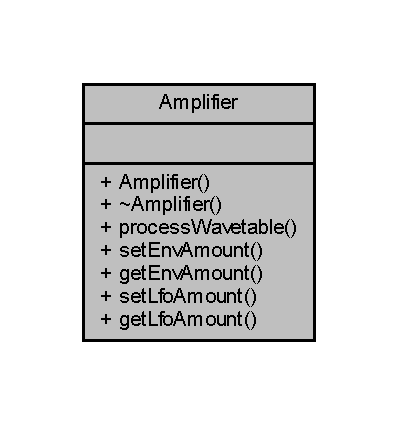
\includegraphics[width=191pt]{df/d37/class_amplifier__coll__graph}
\end{center}
\end{figure}
\subsection*{Public Member Functions}
\begin{DoxyCompactItemize}
\item 
\hyperlink{class_amplifier_ad89ce9e2bd6877057d15266d0d3feb4e}{Amplifier} ()
\item 
\hyperlink{class_amplifier_a6cb2421d049843d6b1994364ea29aabd}{$\sim$\+Amplifier} ()
\item 
void \hyperlink{class_amplifier_a3f1ec0c50fdb0adb71e2f7576e38170a}{process\+Wavetable} (\hyperlink{class_wavetable}{Wavetable} \&source\+Wavetable, char env\+Level, char lfo\+Level)
\item 
void \hyperlink{class_amplifier_a1106605e158c9855d4e303e6972baf9f}{set\+Env\+Amount} (unsigned char new\+Amount)
\item 
unsigned char \hyperlink{class_amplifier_a4cb59ec35a428bf0361799326fbb42c3}{get\+Env\+Amount} ()
\item 
void \hyperlink{class_amplifier_a99593afade53ffadc6958861e38b612a}{set\+Lfo\+Amount} (unsigned char new\+Amount)
\item 
unsigned char \hyperlink{class_amplifier_aeb4c113b992aae7b6fa96fb7ebf9a5ca}{get\+Lfo\+Amount} ()
\end{DoxyCompactItemize}


\subsection{Detailed Description}


Definition at line 23 of file Amplifier.\+h.



\subsection{Constructor \& Destructor Documentation}
\mbox{\Hypertarget{class_amplifier_ad89ce9e2bd6877057d15266d0d3feb4e}\label{class_amplifier_ad89ce9e2bd6877057d15266d0d3feb4e}} 
\index{Amplifier@{Amplifier}!Amplifier@{Amplifier}}
\index{Amplifier@{Amplifier}!Amplifier@{Amplifier}}
\subsubsection{\texorpdfstring{Amplifier()}{Amplifier()}}
{\footnotesize\ttfamily Amplifier\+::\+Amplifier (\begin{DoxyParamCaption}{ }\end{DoxyParamCaption})}



Definition at line 19 of file Amplifier.\+cpp.

Here is the caller graph for this function\+:
\nopagebreak
\begin{figure}[H]
\begin{center}
\leavevmode
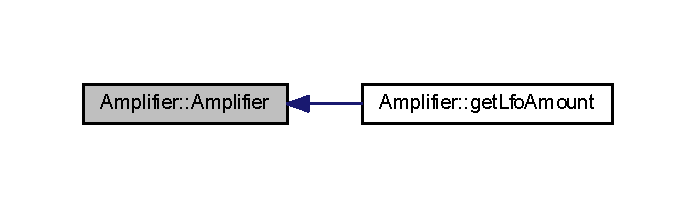
\includegraphics[width=334pt]{de/d01/class_amplifier_ad89ce9e2bd6877057d15266d0d3feb4e_icgraph}
\end{center}
\end{figure}
\mbox{\Hypertarget{class_amplifier_a6cb2421d049843d6b1994364ea29aabd}\label{class_amplifier_a6cb2421d049843d6b1994364ea29aabd}} 
\index{Amplifier@{Amplifier}!````~Amplifier@{$\sim$\+Amplifier}}
\index{````~Amplifier@{$\sim$\+Amplifier}!Amplifier@{Amplifier}}
\subsubsection{\texorpdfstring{$\sim$\+Amplifier()}{~Amplifier()}}
{\footnotesize\ttfamily Amplifier\+::$\sim$\+Amplifier (\begin{DoxyParamCaption}{ }\end{DoxyParamCaption})}



Definition at line 25 of file Amplifier.\+cpp.



\subsection{Member Function Documentation}
\mbox{\Hypertarget{class_amplifier_a4cb59ec35a428bf0361799326fbb42c3}\label{class_amplifier_a4cb59ec35a428bf0361799326fbb42c3}} 
\index{Amplifier@{Amplifier}!get\+Env\+Amount@{get\+Env\+Amount}}
\index{get\+Env\+Amount@{get\+Env\+Amount}!Amplifier@{Amplifier}}
\subsubsection{\texorpdfstring{get\+Env\+Amount()}{getEnvAmount()}}
{\footnotesize\ttfamily unsigned char Amplifier\+::get\+Env\+Amount (\begin{DoxyParamCaption}{ }\end{DoxyParamCaption})\hspace{0.3cm}{\ttfamily [inline]}}



Definition at line 37 of file Amplifier.\+h.

\mbox{\Hypertarget{class_amplifier_aeb4c113b992aae7b6fa96fb7ebf9a5ca}\label{class_amplifier_aeb4c113b992aae7b6fa96fb7ebf9a5ca}} 
\index{Amplifier@{Amplifier}!get\+Lfo\+Amount@{get\+Lfo\+Amount}}
\index{get\+Lfo\+Amount@{get\+Lfo\+Amount}!Amplifier@{Amplifier}}
\subsubsection{\texorpdfstring{get\+Lfo\+Amount()}{getLfoAmount()}}
{\footnotesize\ttfamily unsigned char Amplifier\+::get\+Lfo\+Amount (\begin{DoxyParamCaption}{ }\end{DoxyParamCaption})\hspace{0.3cm}{\ttfamily [inline]}}



Definition at line 39 of file Amplifier.\+h.

Here is the call graph for this function\+:
\nopagebreak
\begin{figure}[H]
\begin{center}
\leavevmode
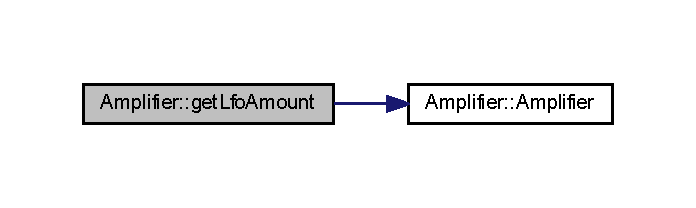
\includegraphics[width=334pt]{de/d01/class_amplifier_aeb4c113b992aae7b6fa96fb7ebf9a5ca_cgraph}
\end{center}
\end{figure}
\mbox{\Hypertarget{class_amplifier_a3f1ec0c50fdb0adb71e2f7576e38170a}\label{class_amplifier_a3f1ec0c50fdb0adb71e2f7576e38170a}} 
\index{Amplifier@{Amplifier}!process\+Wavetable@{process\+Wavetable}}
\index{process\+Wavetable@{process\+Wavetable}!Amplifier@{Amplifier}}
\subsubsection{\texorpdfstring{process\+Wavetable()}{processWavetable()}}
{\footnotesize\ttfamily void Amplifier\+::process\+Wavetable (\begin{DoxyParamCaption}\item[{\hyperlink{class_wavetable}{Wavetable} \&}]{source\+Wavetable,  }\item[{char}]{env\+Level,  }\item[{char}]{lfo\+Level }\end{DoxyParamCaption})}



Definition at line 29 of file Amplifier.\+cpp.

Here is the call graph for this function\+:
\nopagebreak
\begin{figure}[H]
\begin{center}
\leavevmode
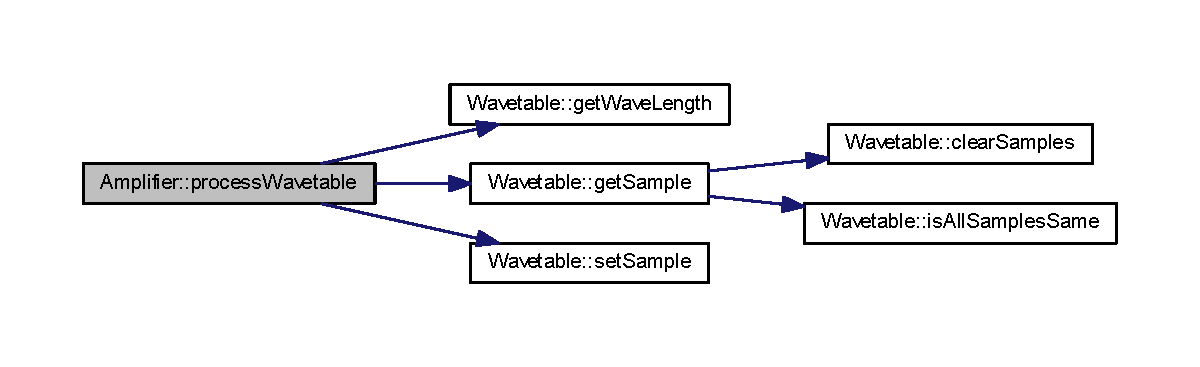
\includegraphics[width=350pt]{de/d01/class_amplifier_a3f1ec0c50fdb0adb71e2f7576e38170a_cgraph}
\end{center}
\end{figure}
Here is the caller graph for this function\+:
\nopagebreak
\begin{figure}[H]
\begin{center}
\leavevmode
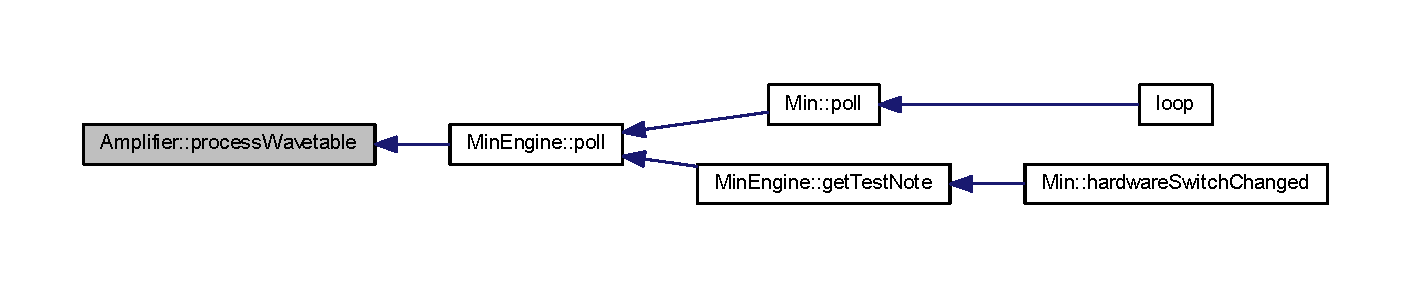
\includegraphics[width=350pt]{de/d01/class_amplifier_a3f1ec0c50fdb0adb71e2f7576e38170a_icgraph}
\end{center}
\end{figure}
\mbox{\Hypertarget{class_amplifier_a1106605e158c9855d4e303e6972baf9f}\label{class_amplifier_a1106605e158c9855d4e303e6972baf9f}} 
\index{Amplifier@{Amplifier}!set\+Env\+Amount@{set\+Env\+Amount}}
\index{set\+Env\+Amount@{set\+Env\+Amount}!Amplifier@{Amplifier}}
\subsubsection{\texorpdfstring{set\+Env\+Amount()}{setEnvAmount()}}
{\footnotesize\ttfamily void Amplifier\+::set\+Env\+Amount (\begin{DoxyParamCaption}\item[{unsigned char}]{new\+Amount }\end{DoxyParamCaption})\hspace{0.3cm}{\ttfamily [inline]}}



Definition at line 36 of file Amplifier.\+h.

Here is the caller graph for this function\+:
\nopagebreak
\begin{figure}[H]
\begin{center}
\leavevmode
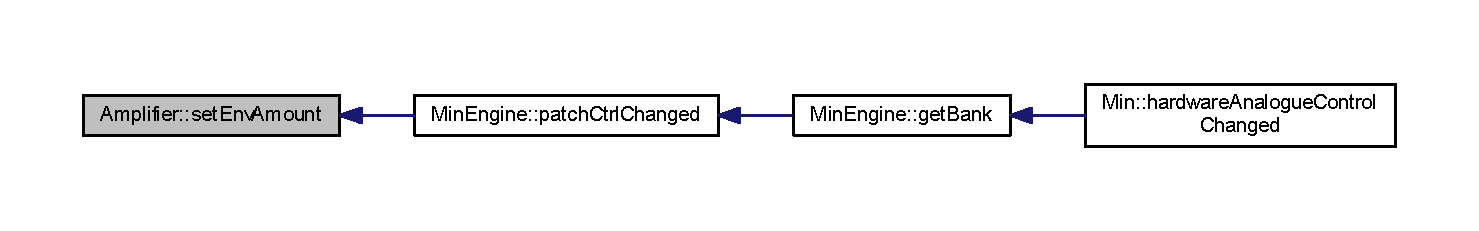
\includegraphics[width=350pt]{de/d01/class_amplifier_a1106605e158c9855d4e303e6972baf9f_icgraph}
\end{center}
\end{figure}
\mbox{\Hypertarget{class_amplifier_a99593afade53ffadc6958861e38b612a}\label{class_amplifier_a99593afade53ffadc6958861e38b612a}} 
\index{Amplifier@{Amplifier}!set\+Lfo\+Amount@{set\+Lfo\+Amount}}
\index{set\+Lfo\+Amount@{set\+Lfo\+Amount}!Amplifier@{Amplifier}}
\subsubsection{\texorpdfstring{set\+Lfo\+Amount()}{setLfoAmount()}}
{\footnotesize\ttfamily void Amplifier\+::set\+Lfo\+Amount (\begin{DoxyParamCaption}\item[{unsigned char}]{new\+Amount }\end{DoxyParamCaption})\hspace{0.3cm}{\ttfamily [inline]}}



Definition at line 38 of file Amplifier.\+h.

Here is the caller graph for this function\+:
\nopagebreak
\begin{figure}[H]
\begin{center}
\leavevmode
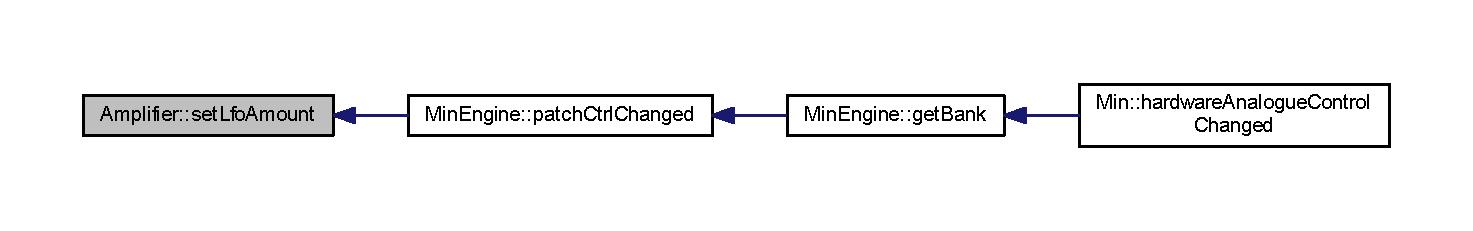
\includegraphics[width=350pt]{de/d01/class_amplifier_a99593afade53ffadc6958861e38b612a_icgraph}
\end{center}
\end{figure}


The documentation for this class was generated from the following files\+:\begin{DoxyCompactItemize}
\item 
\hyperlink{_amplifier_8h}{Amplifier.\+h}\item 
\hyperlink{_amplifier_8cpp}{Amplifier.\+cpp}\end{DoxyCompactItemize}

\hypertarget{class_analogue_control}{}\section{Analogue\+Control Class Reference}
\label{class_analogue_control}\index{Analogue\+Control@{Analogue\+Control}}


{\ttfamily \#include \char`\"{}Analogue\+Control.\+h\char`\"{}}

\subsection*{Public Member Functions}
\begin{DoxyCompactItemize}
\item 
\hyperlink{class_analogue_control_aad4d11c644df1b2b31e32333aceb5d1a}{Analogue\+Control} ()
\item 
\hyperlink{class_analogue_control_a58826c0582ce0697d1c03a92991a648c}{Analogue\+Control} (unsigned char index, unsigned char init\+Value, \hyperlink{class_analogue_control_base}{Analogue\+Control\+Base} $\ast$base)
\item 
\hyperlink{class_analogue_control_af5c00f8da0a5b050a6552e4d111bfe39}{Analogue\+Control} (unsigned char init\+Value)
\item 
\hyperlink{class_analogue_control_a08a12843e8a0a1cb8a0ef9da3865a453}{$\sim$\+Analogue\+Control} ()
\item 
void \hyperlink{class_analogue_control_a160ce73eb8eebdf131dca4dcebc44a42}{set\+Value} (unsigned char new\+Value)
\item 
unsigned char \hyperlink{class_analogue_control_ad92cad38f19cedae45aeeab748ddb455}{get\+Value} ()
\item 
bool \hyperlink{class_analogue_control_a1c2b0439a77656ce62ddc69ee851cb86}{get\+Moving} ()
\item 
void \hyperlink{class_analogue_control_af9129cb76c8fb8ea46e5fea1ea00be73}{set\+Latching} (bool new\+Value)
\item 
bool \hyperlink{class_analogue_control_a69b90c306b7831a3addb30b6683ec171}{get\+Latching} ()
\item 
void \hyperlink{class_analogue_control_a3dd85b57a3fe8eceddcd2e4bbfce1ea9}{set\+Latched} (bool new\+Value)
\item 
bool \hyperlink{class_analogue_control_a0fd8ee45aa916be0b7ba0bdccab41033}{get\+Latched} ()
\item 
bool \hyperlink{class_analogue_control_ab670265f948d7416bcf07c91dcf97bce}{has\+Changed} (unsigned char ticks\+Passed)
\item 
void \hyperlink{class_analogue_control_a5ec0b55a6abd8c73e61f86f2322251a5}{poll} (unsigned char ticks\+Passed)
\end{DoxyCompactItemize}


\subsection{Detailed Description}


Definition at line 23 of file Analogue\+Control.\+h.



\subsection{Constructor \& Destructor Documentation}
\mbox{\Hypertarget{class_analogue_control_aad4d11c644df1b2b31e32333aceb5d1a}\label{class_analogue_control_aad4d11c644df1b2b31e32333aceb5d1a}} 
\index{Analogue\+Control@{Analogue\+Control}!Analogue\+Control@{Analogue\+Control}}
\index{Analogue\+Control@{Analogue\+Control}!Analogue\+Control@{Analogue\+Control}}
\subsubsection{\texorpdfstring{Analogue\+Control()}{AnalogueControl()}\hspace{0.1cm}{\footnotesize\ttfamily [1/3]}}
{\footnotesize\ttfamily Analogue\+Control\+::\+Analogue\+Control (\begin{DoxyParamCaption}{ }\end{DoxyParamCaption})\hspace{0.3cm}{\ttfamily [inline]}}



Definition at line 42 of file Analogue\+Control.\+h.

Here is the call graph for this function\+:
\nopagebreak
\begin{figure}[H]
\begin{center}
\leavevmode
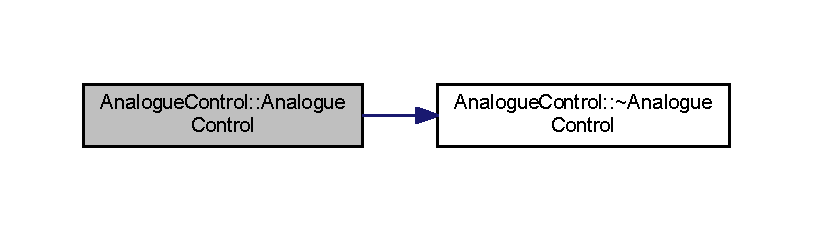
\includegraphics[width=350pt]{class_analogue_control_aad4d11c644df1b2b31e32333aceb5d1a_cgraph}
\end{center}
\end{figure}
\mbox{\Hypertarget{class_analogue_control_a58826c0582ce0697d1c03a92991a648c}\label{class_analogue_control_a58826c0582ce0697d1c03a92991a648c}} 
\index{Analogue\+Control@{Analogue\+Control}!Analogue\+Control@{Analogue\+Control}}
\index{Analogue\+Control@{Analogue\+Control}!Analogue\+Control@{Analogue\+Control}}
\subsubsection{\texorpdfstring{Analogue\+Control()}{AnalogueControl()}\hspace{0.1cm}{\footnotesize\ttfamily [2/3]}}
{\footnotesize\ttfamily Analogue\+Control\+::\+Analogue\+Control (\begin{DoxyParamCaption}\item[{unsigned char}]{index,  }\item[{unsigned char}]{init\+Value,  }\item[{\hyperlink{class_analogue_control_base}{Analogue\+Control\+Base} $\ast$}]{base }\end{DoxyParamCaption})}



Definition at line 26 of file Analogue\+Control.\+cpp.

\mbox{\Hypertarget{class_analogue_control_af5c00f8da0a5b050a6552e4d111bfe39}\label{class_analogue_control_af5c00f8da0a5b050a6552e4d111bfe39}} 
\index{Analogue\+Control@{Analogue\+Control}!Analogue\+Control@{Analogue\+Control}}
\index{Analogue\+Control@{Analogue\+Control}!Analogue\+Control@{Analogue\+Control}}
\subsubsection{\texorpdfstring{Analogue\+Control()}{AnalogueControl()}\hspace{0.1cm}{\footnotesize\ttfamily [3/3]}}
{\footnotesize\ttfamily Analogue\+Control\+::\+Analogue\+Control (\begin{DoxyParamCaption}\item[{unsigned char}]{init\+Value }\end{DoxyParamCaption})}



Definition at line 20 of file Analogue\+Control.\+cpp.

\mbox{\Hypertarget{class_analogue_control_a08a12843e8a0a1cb8a0ef9da3865a453}\label{class_analogue_control_a08a12843e8a0a1cb8a0ef9da3865a453}} 
\index{Analogue\+Control@{Analogue\+Control}!````~Analogue\+Control@{$\sim$\+Analogue\+Control}}
\index{````~Analogue\+Control@{$\sim$\+Analogue\+Control}!Analogue\+Control@{Analogue\+Control}}
\subsubsection{\texorpdfstring{$\sim$\+Analogue\+Control()}{~AnalogueControl()}}
{\footnotesize\ttfamily Analogue\+Control\+::$\sim$\+Analogue\+Control (\begin{DoxyParamCaption}{ }\end{DoxyParamCaption})}



Definition at line 38 of file Analogue\+Control.\+cpp.

Here is the caller graph for this function\+:
\nopagebreak
\begin{figure}[H]
\begin{center}
\leavevmode
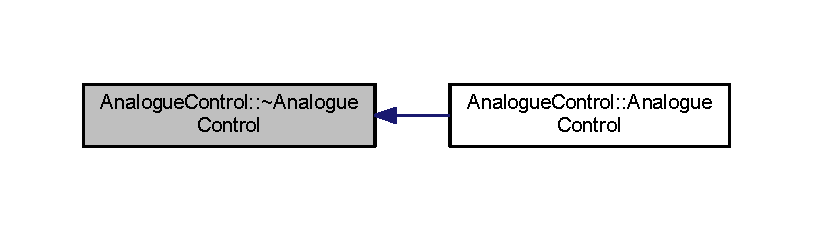
\includegraphics[width=350pt]{class_analogue_control_a08a12843e8a0a1cb8a0ef9da3865a453_icgraph}
\end{center}
\end{figure}


\subsection{Member Function Documentation}
\mbox{\Hypertarget{class_analogue_control_a0fd8ee45aa916be0b7ba0bdccab41033}\label{class_analogue_control_a0fd8ee45aa916be0b7ba0bdccab41033}} 
\index{Analogue\+Control@{Analogue\+Control}!get\+Latched@{get\+Latched}}
\index{get\+Latched@{get\+Latched}!Analogue\+Control@{Analogue\+Control}}
\subsubsection{\texorpdfstring{get\+Latched()}{getLatched()}}
{\footnotesize\ttfamily bool Analogue\+Control\+::get\+Latched (\begin{DoxyParamCaption}{ }\end{DoxyParamCaption})\hspace{0.3cm}{\ttfamily [inline]}}



Definition at line 52 of file Analogue\+Control.\+h.

Here is the call graph for this function\+:
\nopagebreak
\begin{figure}[H]
\begin{center}
\leavevmode
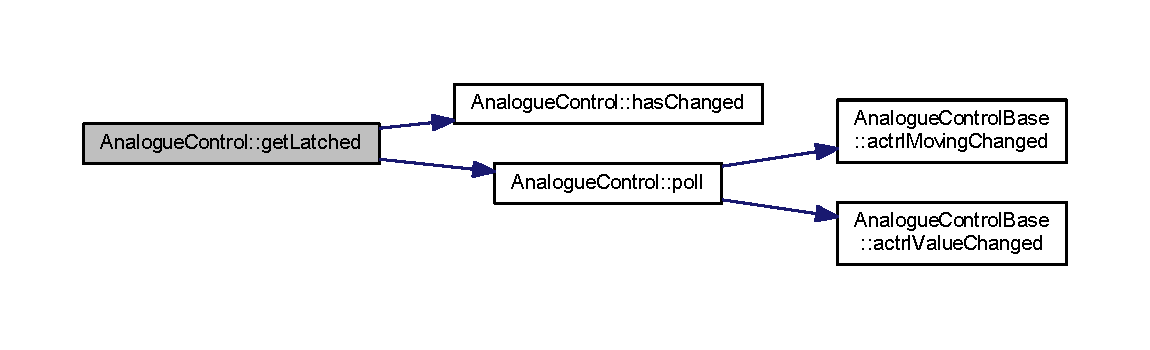
\includegraphics[width=350pt]{class_analogue_control_a0fd8ee45aa916be0b7ba0bdccab41033_cgraph}
\end{center}
\end{figure}
\mbox{\Hypertarget{class_analogue_control_a69b90c306b7831a3addb30b6683ec171}\label{class_analogue_control_a69b90c306b7831a3addb30b6683ec171}} 
\index{Analogue\+Control@{Analogue\+Control}!get\+Latching@{get\+Latching}}
\index{get\+Latching@{get\+Latching}!Analogue\+Control@{Analogue\+Control}}
\subsubsection{\texorpdfstring{get\+Latching()}{getLatching()}}
{\footnotesize\ttfamily bool Analogue\+Control\+::get\+Latching (\begin{DoxyParamCaption}{ }\end{DoxyParamCaption})\hspace{0.3cm}{\ttfamily [inline]}}



Definition at line 50 of file Analogue\+Control.\+h.

\mbox{\Hypertarget{class_analogue_control_a1c2b0439a77656ce62ddc69ee851cb86}\label{class_analogue_control_a1c2b0439a77656ce62ddc69ee851cb86}} 
\index{Analogue\+Control@{Analogue\+Control}!get\+Moving@{get\+Moving}}
\index{get\+Moving@{get\+Moving}!Analogue\+Control@{Analogue\+Control}}
\subsubsection{\texorpdfstring{get\+Moving()}{getMoving()}}
{\footnotesize\ttfamily bool Analogue\+Control\+::get\+Moving (\begin{DoxyParamCaption}{ }\end{DoxyParamCaption})\hspace{0.3cm}{\ttfamily [inline]}}



Definition at line 48 of file Analogue\+Control.\+h.

\mbox{\Hypertarget{class_analogue_control_ad92cad38f19cedae45aeeab748ddb455}\label{class_analogue_control_ad92cad38f19cedae45aeeab748ddb455}} 
\index{Analogue\+Control@{Analogue\+Control}!get\+Value@{get\+Value}}
\index{get\+Value@{get\+Value}!Analogue\+Control@{Analogue\+Control}}
\subsubsection{\texorpdfstring{get\+Value()}{getValue()}}
{\footnotesize\ttfamily unsigned char Analogue\+Control\+::get\+Value (\begin{DoxyParamCaption}{ }\end{DoxyParamCaption})\hspace{0.3cm}{\ttfamily [inline]}}



Definition at line 47 of file Analogue\+Control.\+h.

\mbox{\Hypertarget{class_analogue_control_ab670265f948d7416bcf07c91dcf97bce}\label{class_analogue_control_ab670265f948d7416bcf07c91dcf97bce}} 
\index{Analogue\+Control@{Analogue\+Control}!has\+Changed@{has\+Changed}}
\index{has\+Changed@{has\+Changed}!Analogue\+Control@{Analogue\+Control}}
\subsubsection{\texorpdfstring{has\+Changed()}{hasChanged()}}
{\footnotesize\ttfamily bool Analogue\+Control\+::has\+Changed (\begin{DoxyParamCaption}\item[{unsigned char}]{ticks\+Passed }\end{DoxyParamCaption})}



Definition at line 46 of file Analogue\+Control.\+cpp.

Here is the caller graph for this function\+:
\nopagebreak
\begin{figure}[H]
\begin{center}
\leavevmode
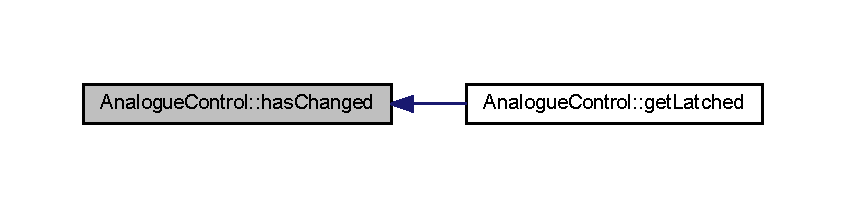
\includegraphics[width=350pt]{class_analogue_control_ab670265f948d7416bcf07c91dcf97bce_icgraph}
\end{center}
\end{figure}
\mbox{\Hypertarget{class_analogue_control_a5ec0b55a6abd8c73e61f86f2322251a5}\label{class_analogue_control_a5ec0b55a6abd8c73e61f86f2322251a5}} 
\index{Analogue\+Control@{Analogue\+Control}!poll@{poll}}
\index{poll@{poll}!Analogue\+Control@{Analogue\+Control}}
\subsubsection{\texorpdfstring{poll()}{poll()}}
{\footnotesize\ttfamily void Analogue\+Control\+::poll (\begin{DoxyParamCaption}\item[{unsigned char}]{ticks\+Passed }\end{DoxyParamCaption})}



Definition at line 76 of file Analogue\+Control.\+cpp.

Here is the call graph for this function\+:
\nopagebreak
\begin{figure}[H]
\begin{center}
\leavevmode
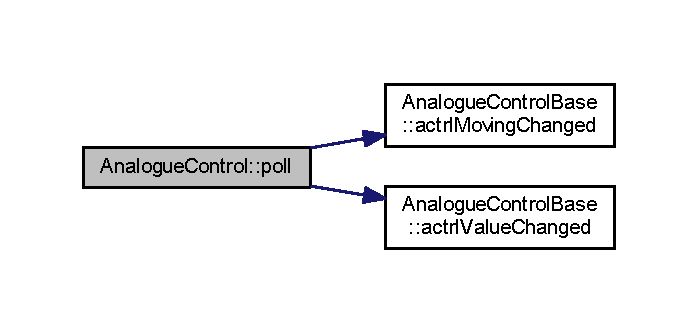
\includegraphics[width=335pt]{class_analogue_control_a5ec0b55a6abd8c73e61f86f2322251a5_cgraph}
\end{center}
\end{figure}
Here is the caller graph for this function\+:
\nopagebreak
\begin{figure}[H]
\begin{center}
\leavevmode
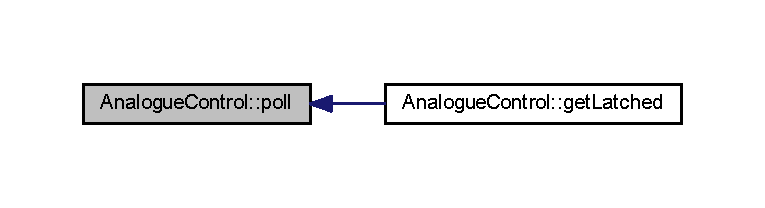
\includegraphics[width=350pt]{class_analogue_control_a5ec0b55a6abd8c73e61f86f2322251a5_icgraph}
\end{center}
\end{figure}
\mbox{\Hypertarget{class_analogue_control_a3dd85b57a3fe8eceddcd2e4bbfce1ea9}\label{class_analogue_control_a3dd85b57a3fe8eceddcd2e4bbfce1ea9}} 
\index{Analogue\+Control@{Analogue\+Control}!set\+Latched@{set\+Latched}}
\index{set\+Latched@{set\+Latched}!Analogue\+Control@{Analogue\+Control}}
\subsubsection{\texorpdfstring{set\+Latched()}{setLatched()}}
{\footnotesize\ttfamily void Analogue\+Control\+::set\+Latched (\begin{DoxyParamCaption}\item[{bool}]{new\+Value }\end{DoxyParamCaption})\hspace{0.3cm}{\ttfamily [inline]}}



Definition at line 51 of file Analogue\+Control.\+h.

\mbox{\Hypertarget{class_analogue_control_af9129cb76c8fb8ea46e5fea1ea00be73}\label{class_analogue_control_af9129cb76c8fb8ea46e5fea1ea00be73}} 
\index{Analogue\+Control@{Analogue\+Control}!set\+Latching@{set\+Latching}}
\index{set\+Latching@{set\+Latching}!Analogue\+Control@{Analogue\+Control}}
\subsubsection{\texorpdfstring{set\+Latching()}{setLatching()}}
{\footnotesize\ttfamily void Analogue\+Control\+::set\+Latching (\begin{DoxyParamCaption}\item[{bool}]{new\+Value }\end{DoxyParamCaption})\hspace{0.3cm}{\ttfamily [inline]}}



Definition at line 49 of file Analogue\+Control.\+h.

\mbox{\Hypertarget{class_analogue_control_a160ce73eb8eebdf131dca4dcebc44a42}\label{class_analogue_control_a160ce73eb8eebdf131dca4dcebc44a42}} 
\index{Analogue\+Control@{Analogue\+Control}!set\+Value@{set\+Value}}
\index{set\+Value@{set\+Value}!Analogue\+Control@{Analogue\+Control}}
\subsubsection{\texorpdfstring{set\+Value()}{setValue()}}
{\footnotesize\ttfamily void Analogue\+Control\+::set\+Value (\begin{DoxyParamCaption}\item[{unsigned char}]{new\+Value }\end{DoxyParamCaption})\hspace{0.3cm}{\ttfamily [inline]}}



Definition at line 46 of file Analogue\+Control.\+h.

Here is the caller graph for this function\+:
\nopagebreak
\begin{figure}[H]
\begin{center}
\leavevmode
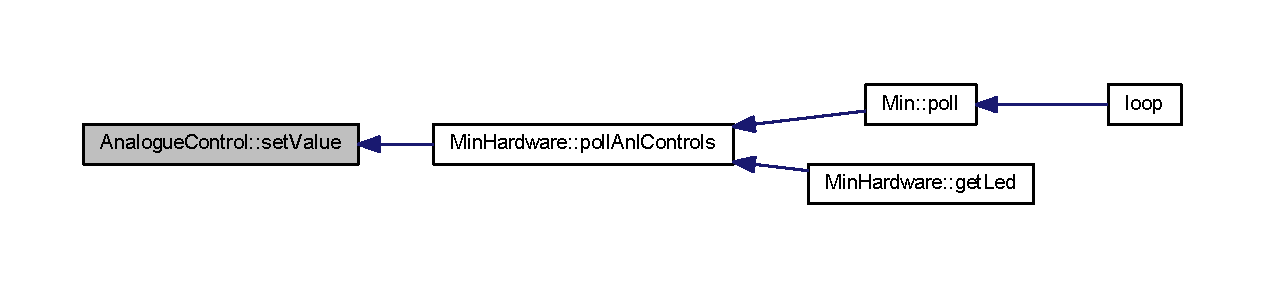
\includegraphics[width=350pt]{class_analogue_control_a160ce73eb8eebdf131dca4dcebc44a42_icgraph}
\end{center}
\end{figure}


The documentation for this class was generated from the following files\+:\begin{DoxyCompactItemize}
\item 
\hyperlink{_analogue_control_8h}{Analogue\+Control.\+h}\item 
\hyperlink{_analogue_control_8cpp}{Analogue\+Control.\+cpp}\end{DoxyCompactItemize}

\hypertarget{class_analogue_control_base}{}\section{Analogue\+Control\+Base Class Reference}
\label{class_analogue_control_base}\index{Analogue\+Control\+Base@{Analogue\+Control\+Base}}


{\ttfamily \#include \char`\"{}Analogue\+Control\+Base.\+h\char`\"{}}

\subsection*{Public Member Functions}
\begin{DoxyCompactItemize}
\item 
virtual void \hyperlink{class_analogue_control_base_a9d18c3e299a69c909a3ad88b70524c5d}{actrl\+Value\+Changed} (unsigned char index, unsigned char new\+Value)=0
\item 
virtual void \hyperlink{class_analogue_control_base_ab680f6fd45ec093200d3d78744957c1b}{actrl\+Moving\+Changed} (unsigned char index, bool new\+Value)=0
\end{DoxyCompactItemize}


\subsection{Detailed Description}


Definition at line 21 of file Analogue\+Control\+Base.\+h.



\subsection{Member Function Documentation}
\mbox{\Hypertarget{class_analogue_control_base_ab680f6fd45ec093200d3d78744957c1b}\label{class_analogue_control_base_ab680f6fd45ec093200d3d78744957c1b}} 
\index{Analogue\+Control\+Base@{Analogue\+Control\+Base}!actrl\+Moving\+Changed@{actrl\+Moving\+Changed}}
\index{actrl\+Moving\+Changed@{actrl\+Moving\+Changed}!Analogue\+Control\+Base@{Analogue\+Control\+Base}}
\subsubsection{\texorpdfstring{actrl\+Moving\+Changed()}{actrlMovingChanged()}}
{\footnotesize\ttfamily virtual void Analogue\+Control\+Base\+::actrl\+Moving\+Changed (\begin{DoxyParamCaption}\item[{unsigned char}]{index,  }\item[{bool}]{new\+Value }\end{DoxyParamCaption})\hspace{0.3cm}{\ttfamily [pure virtual]}}

Here is the caller graph for this function\+:
\nopagebreak
\begin{figure}[H]
\begin{center}
\leavevmode
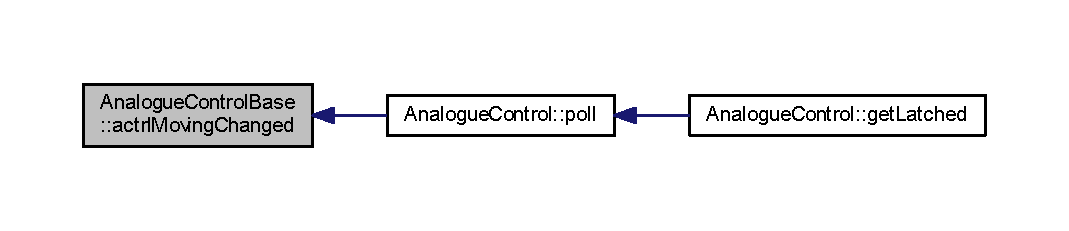
\includegraphics[width=350pt]{class_analogue_control_base_ab680f6fd45ec093200d3d78744957c1b_icgraph}
\end{center}
\end{figure}
\mbox{\Hypertarget{class_analogue_control_base_a9d18c3e299a69c909a3ad88b70524c5d}\label{class_analogue_control_base_a9d18c3e299a69c909a3ad88b70524c5d}} 
\index{Analogue\+Control\+Base@{Analogue\+Control\+Base}!actrl\+Value\+Changed@{actrl\+Value\+Changed}}
\index{actrl\+Value\+Changed@{actrl\+Value\+Changed}!Analogue\+Control\+Base@{Analogue\+Control\+Base}}
\subsubsection{\texorpdfstring{actrl\+Value\+Changed()}{actrlValueChanged()}}
{\footnotesize\ttfamily virtual void Analogue\+Control\+Base\+::actrl\+Value\+Changed (\begin{DoxyParamCaption}\item[{unsigned char}]{index,  }\item[{unsigned char}]{new\+Value }\end{DoxyParamCaption})\hspace{0.3cm}{\ttfamily [pure virtual]}}

Here is the caller graph for this function\+:
\nopagebreak
\begin{figure}[H]
\begin{center}
\leavevmode
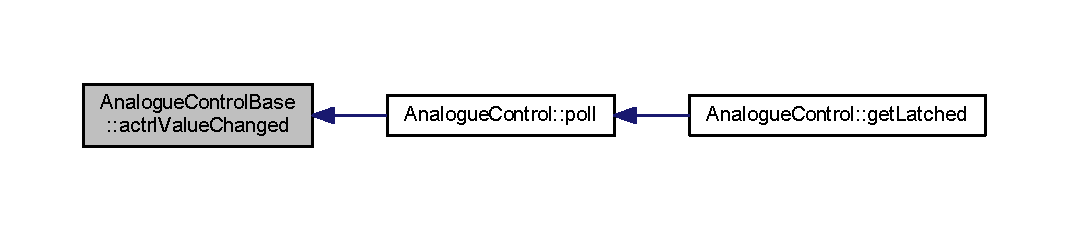
\includegraphics[width=350pt]{class_analogue_control_base_a9d18c3e299a69c909a3ad88b70524c5d_icgraph}
\end{center}
\end{figure}


The documentation for this class was generated from the following file\+:\begin{DoxyCompactItemize}
\item 
\hyperlink{_analogue_control_base_8h}{Analogue\+Control\+Base.\+h}\end{DoxyCompactItemize}

\hypertarget{class_atm_audio}{}\section{Atm\+Audio Class Reference}
\label{class_atm_audio}\index{Atm\+Audio@{Atm\+Audio}}


{\ttfamily \#include \char`\"{}Atm\+Audio.\+h\char`\"{}}

\subsection*{Public Member Functions}
\begin{DoxyCompactItemize}
\item 
\hyperlink{class_atm_audio_adef4ded5a0c213fe421025e17de0605e}{Atm\+Audio} (unsigned char wave\+Len)
\item 
\hyperlink{class_atm_audio_ad4d285853a6790f23fd8dd24998a830b}{$\sim$\+Atm\+Audio} ()
\item 
void \hyperlink{class_atm_audio_ab27c4dabb9e47a386de693b47422bb2a}{set\+Sample\+Freq} (unsigned long new\+Sf)
\item 
unsigned long \hyperlink{class_atm_audio_a9336911a6a8dd22d4030b0457270c242}{get\+Sample\+Freq} ()
\item 
void \hyperlink{class_atm_audio_a3944db83a92a88144603c78b0260463a}{paste\+Wavetable} (\hyperlink{class_wavetable}{Wavetable} \&source\+Wavetable)
\item 
void \hyperlink{class_atm_audio_ab634d78d1e88550a4ed0ff1d93ed2d97}{resize\+Wavetable} (unsigned char new\+Wave\+Len)
\end{DoxyCompactItemize}
\subsection*{Static Public Member Functions}
\begin{DoxyCompactItemize}
\item 
static void \hyperlink{class_atm_audio_ada27d4d2556b8b27f4c3c8b4da763176}{initialize} ()
\end{DoxyCompactItemize}


\subsection{Detailed Description}


Definition at line 40 of file Atm\+Audio.\+h.



\subsection{Constructor \& Destructor Documentation}
\mbox{\Hypertarget{class_atm_audio_adef4ded5a0c213fe421025e17de0605e}\label{class_atm_audio_adef4ded5a0c213fe421025e17de0605e}} 
\index{Atm\+Audio@{Atm\+Audio}!Atm\+Audio@{Atm\+Audio}}
\index{Atm\+Audio@{Atm\+Audio}!Atm\+Audio@{Atm\+Audio}}
\subsubsection{\texorpdfstring{Atm\+Audio()}{AtmAudio()}}
{\footnotesize\ttfamily Atm\+Audio\+::\+Atm\+Audio (\begin{DoxyParamCaption}\item[{unsigned char}]{wave\+Len }\end{DoxyParamCaption})}



Definition at line 32 of file Atm\+Audio.\+cpp.

Here is the call graph for this function\+:
\nopagebreak
\begin{figure}[H]
\begin{center}
\leavevmode
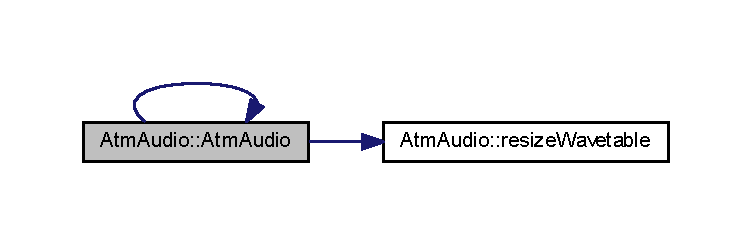
\includegraphics[width=350pt]{class_atm_audio_adef4ded5a0c213fe421025e17de0605e_cgraph}
\end{center}
\end{figure}
Here is the caller graph for this function\+:
\nopagebreak
\begin{figure}[H]
\begin{center}
\leavevmode
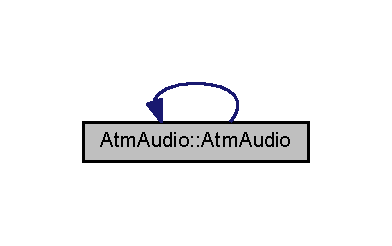
\includegraphics[width=188pt]{class_atm_audio_adef4ded5a0c213fe421025e17de0605e_icgraph}
\end{center}
\end{figure}
\mbox{\Hypertarget{class_atm_audio_ad4d285853a6790f23fd8dd24998a830b}\label{class_atm_audio_ad4d285853a6790f23fd8dd24998a830b}} 
\index{Atm\+Audio@{Atm\+Audio}!````~Atm\+Audio@{$\sim$\+Atm\+Audio}}
\index{````~Atm\+Audio@{$\sim$\+Atm\+Audio}!Atm\+Audio@{Atm\+Audio}}
\subsubsection{\texorpdfstring{$\sim$\+Atm\+Audio()}{~AtmAudio()}}
{\footnotesize\ttfamily Atm\+Audio\+::$\sim$\+Atm\+Audio (\begin{DoxyParamCaption}{ }\end{DoxyParamCaption})}



Definition at line 42 of file Atm\+Audio.\+cpp.



\subsection{Member Function Documentation}
\mbox{\Hypertarget{class_atm_audio_a9336911a6a8dd22d4030b0457270c242}\label{class_atm_audio_a9336911a6a8dd22d4030b0457270c242}} 
\index{Atm\+Audio@{Atm\+Audio}!get\+Sample\+Freq@{get\+Sample\+Freq}}
\index{get\+Sample\+Freq@{get\+Sample\+Freq}!Atm\+Audio@{Atm\+Audio}}
\subsubsection{\texorpdfstring{get\+Sample\+Freq()}{getSampleFreq()}}
{\footnotesize\ttfamily unsigned long Atm\+Audio\+::get\+Sample\+Freq (\begin{DoxyParamCaption}{ }\end{DoxyParamCaption})\hspace{0.3cm}{\ttfamily [inline]}}



Definition at line 53 of file Atm\+Audio.\+h.

Here is the call graph for this function\+:
\nopagebreak
\begin{figure}[H]
\begin{center}
\leavevmode
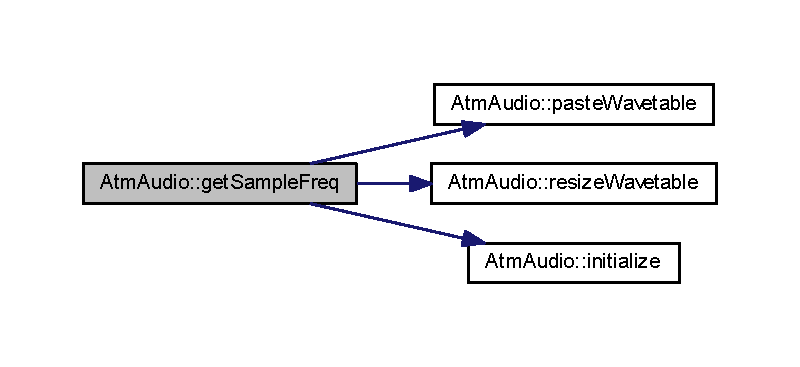
\includegraphics[width=350pt]{class_atm_audio_a9336911a6a8dd22d4030b0457270c242_cgraph}
\end{center}
\end{figure}
Here is the caller graph for this function\+:
\nopagebreak
\begin{figure}[H]
\begin{center}
\leavevmode
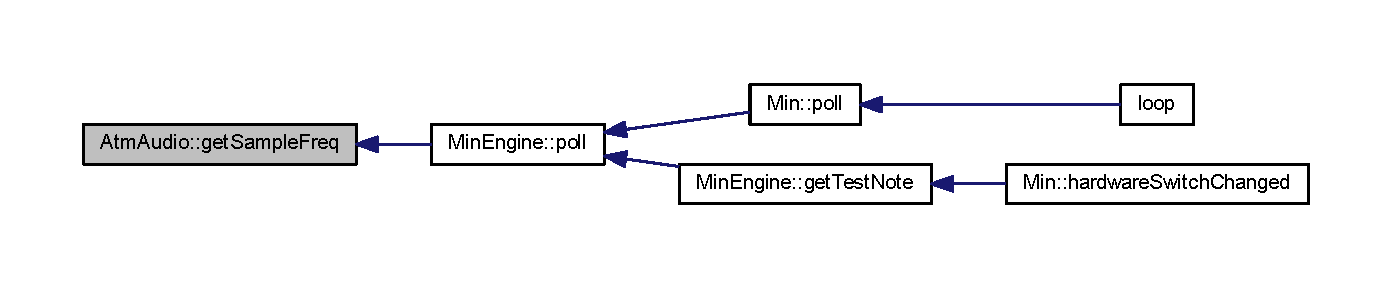
\includegraphics[width=350pt]{class_atm_audio_a9336911a6a8dd22d4030b0457270c242_icgraph}
\end{center}
\end{figure}
\mbox{\Hypertarget{class_atm_audio_ada27d4d2556b8b27f4c3c8b4da763176}\label{class_atm_audio_ada27d4d2556b8b27f4c3c8b4da763176}} 
\index{Atm\+Audio@{Atm\+Audio}!initialize@{initialize}}
\index{initialize@{initialize}!Atm\+Audio@{Atm\+Audio}}
\subsubsection{\texorpdfstring{initialize()}{initialize()}}
{\footnotesize\ttfamily void Atm\+Audio\+::initialize (\begin{DoxyParamCaption}{ }\end{DoxyParamCaption})\hspace{0.3cm}{\ttfamily [static]}}



Definition at line 56 of file Atm\+Audio.\+cpp.

Here is the caller graph for this function\+:
\nopagebreak
\begin{figure}[H]
\begin{center}
\leavevmode
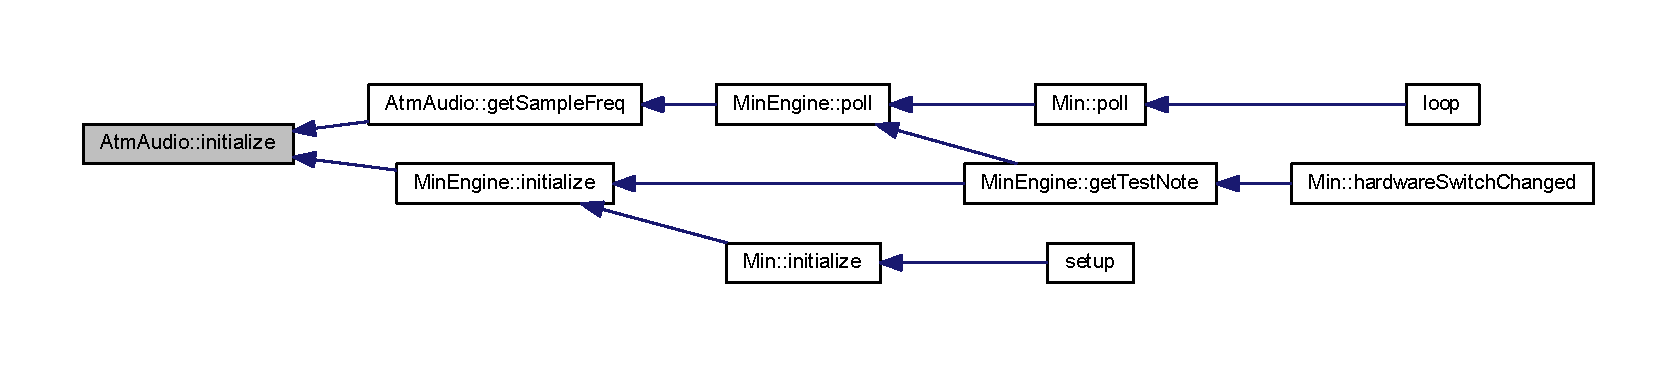
\includegraphics[width=350pt]{class_atm_audio_ada27d4d2556b8b27f4c3c8b4da763176_icgraph}
\end{center}
\end{figure}
\mbox{\Hypertarget{class_atm_audio_a3944db83a92a88144603c78b0260463a}\label{class_atm_audio_a3944db83a92a88144603c78b0260463a}} 
\index{Atm\+Audio@{Atm\+Audio}!paste\+Wavetable@{paste\+Wavetable}}
\index{paste\+Wavetable@{paste\+Wavetable}!Atm\+Audio@{Atm\+Audio}}
\subsubsection{\texorpdfstring{paste\+Wavetable()}{pasteWavetable()}}
{\footnotesize\ttfamily void Atm\+Audio\+::paste\+Wavetable (\begin{DoxyParamCaption}\item[{\hyperlink{class_wavetable}{Wavetable} \&}]{source\+Wavetable }\end{DoxyParamCaption})}



Definition at line 139 of file Atm\+Audio.\+cpp.

Here is the caller graph for this function\+:
\nopagebreak
\begin{figure}[H]
\begin{center}
\leavevmode
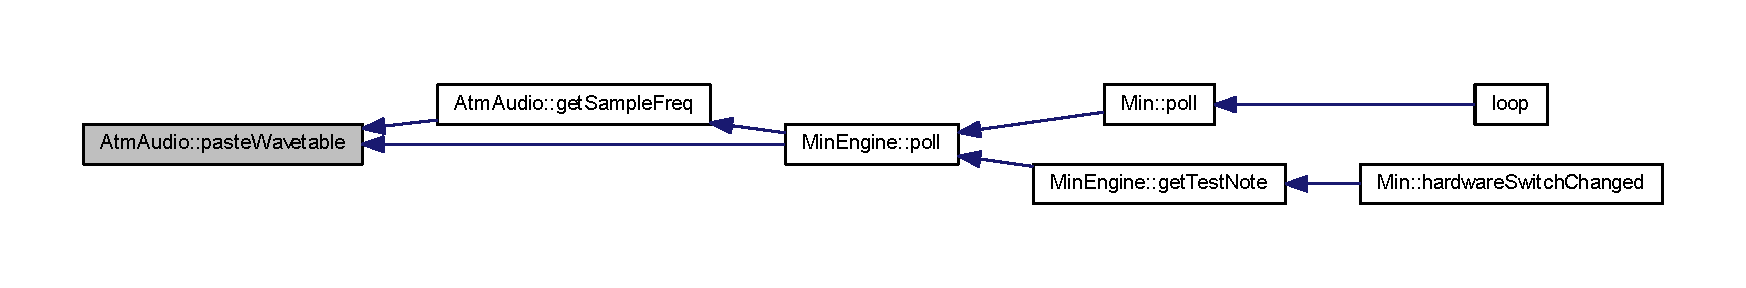
\includegraphics[width=350pt]{class_atm_audio_a3944db83a92a88144603c78b0260463a_icgraph}
\end{center}
\end{figure}
\mbox{\Hypertarget{class_atm_audio_ab634d78d1e88550a4ed0ff1d93ed2d97}\label{class_atm_audio_ab634d78d1e88550a4ed0ff1d93ed2d97}} 
\index{Atm\+Audio@{Atm\+Audio}!resize\+Wavetable@{resize\+Wavetable}}
\index{resize\+Wavetable@{resize\+Wavetable}!Atm\+Audio@{Atm\+Audio}}
\subsubsection{\texorpdfstring{resize\+Wavetable()}{resizeWavetable()}}
{\footnotesize\ttfamily void Atm\+Audio\+::resize\+Wavetable (\begin{DoxyParamCaption}\item[{unsigned char}]{new\+Wave\+Len }\end{DoxyParamCaption})}



Definition at line 133 of file Atm\+Audio.\+cpp.

Here is the caller graph for this function\+:
\nopagebreak
\begin{figure}[H]
\begin{center}
\leavevmode
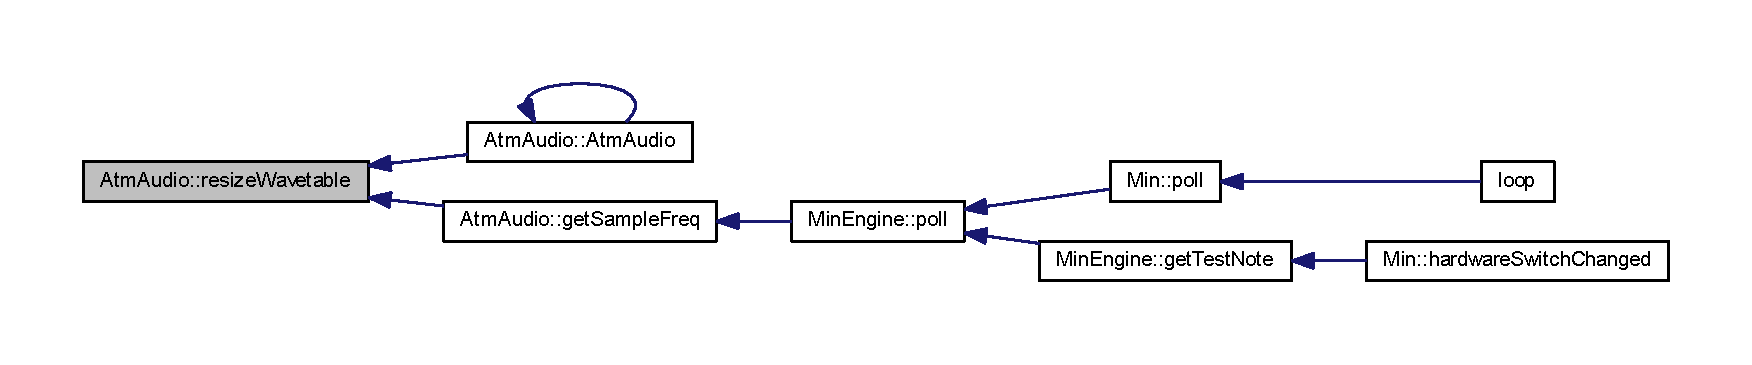
\includegraphics[width=350pt]{class_atm_audio_ab634d78d1e88550a4ed0ff1d93ed2d97_icgraph}
\end{center}
\end{figure}
\mbox{\Hypertarget{class_atm_audio_ab27c4dabb9e47a386de693b47422bb2a}\label{class_atm_audio_ab27c4dabb9e47a386de693b47422bb2a}} 
\index{Atm\+Audio@{Atm\+Audio}!set\+Sample\+Freq@{set\+Sample\+Freq}}
\index{set\+Sample\+Freq@{set\+Sample\+Freq}!Atm\+Audio@{Atm\+Audio}}
\subsubsection{\texorpdfstring{set\+Sample\+Freq()}{setSampleFreq()}}
{\footnotesize\ttfamily void Atm\+Audio\+::set\+Sample\+Freq (\begin{DoxyParamCaption}\item[{unsigned long}]{new\+Sf }\end{DoxyParamCaption})}



Definition at line 103 of file Atm\+Audio.\+cpp.

Here is the caller graph for this function\+:
\nopagebreak
\begin{figure}[H]
\begin{center}
\leavevmode
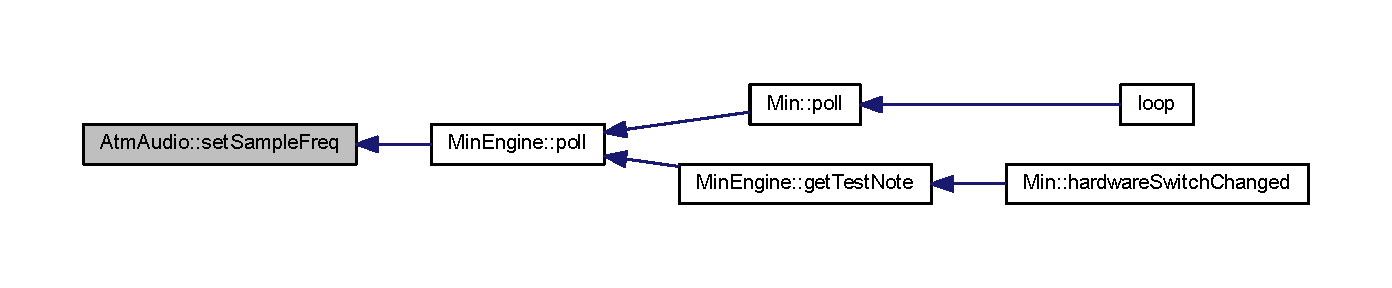
\includegraphics[width=350pt]{class_atm_audio_ab27c4dabb9e47a386de693b47422bb2a_icgraph}
\end{center}
\end{figure}


The documentation for this class was generated from the following files\+:\begin{DoxyCompactItemize}
\item 
\hyperlink{_atm_audio_8h}{Atm\+Audio.\+h}\item 
\hyperlink{_atm_audio_8cpp}{Atm\+Audio.\+cpp}\end{DoxyCompactItemize}

\hypertarget{class_atm_oscillator}{}\section{Atm\+Oscillator Class Reference}
\label{class_atm_oscillator}\index{Atm\+Oscillator@{Atm\+Oscillator}}


{\ttfamily \#include \char`\"{}Atm\+Oscillator.\+h\char`\"{}}

\subsection*{Public Member Functions}
\begin{DoxyCompactItemize}
\item 
\hyperlink{class_atm_oscillator_a864b35c83864a6d5045f9dbb42fa862e}{Atm\+Oscillator} (unsigned char wave\+Length, unsigned int user\+Wave\+Start\+Address)
\item 
\hyperlink{class_atm_oscillator_a3d5b959eff3a2cb4fa3200cadeb2ab0b}{$\sim$\+Atm\+Oscillator} ()
\item 
void \hyperlink{class_atm_oscillator_ab0b1ab90e227ced30ddffff96bec6427}{copy\+Wavetable} (\hyperlink{class_wavetable}{Wavetable} \&dest\+Wavetable)
\item 
void \hyperlink{class_atm_oscillator_ac4248a3cd6fceea6ee677e74faba4af0}{set\+Table} (unsigned char new\+Table)
\item 
unsigned char \hyperlink{class_atm_oscillator_a01e9856e38a1e83b5d83fd503d5ad80e}{get\+Table} ()
\item 
void \hyperlink{class_atm_oscillator_a9f65ae9f2132c46f73b776a869b5bf21}{set\+Bank} (unsigned char new\+Bank)
\item 
unsigned char \hyperlink{class_atm_oscillator_a56b407e4175f4625e2e0d7a6f87c2225}{get\+Bank} ()
\item 
void \hyperlink{class_atm_oscillator_aafaccbb54d52f2c0eb07eb968498eef4}{set\+User\+Mode} (bool new\+User\+Mode)
\item 
bool \hyperlink{class_atm_oscillator_a21a4425606aa28eabf47a28ea7f02c9a}{get\+User\+Mode} ()
\item 
unsigned char \hyperlink{class_atm_oscillator_ad846116dfd6f232cae79ada35dddadfd}{get\+Wave\+Length} ()
\item 
void \hyperlink{class_atm_oscillator_aa62dba14693f65adcb3daa7aa4757ba1}{set\+User\+Wavetable\+Sample} (unsigned char index, char new\+Sample)
\item 
char \hyperlink{class_atm_oscillator_ae5ef1556ef77dbf9ecceb5b64a1ad7e8}{get\+User\+Wavetable\+Sample} (unsigned char index)
\item 
char \hyperlink{class_atm_oscillator_aa6fe7de8b2d573159271a47f5c8686e1}{get\+Sample} (unsigned char index)
\item 
unsigned int \hyperlink{class_atm_oscillator_a19bdaa400d57eeb24ca027febc2fd1cf}{get\+User\+Wave\+Start\+Address} ()
\item 
void \hyperlink{class_atm_oscillator_a92133ff9c3b34a6acb703f0d6d95cd71}{write\+User\+Wave} (unsigned char wave\+Num)
\item 
void \hyperlink{class_atm_oscillator_a08b383cd2305c232de827399aa8d2ccb}{read\+User\+Wave} (unsigned char wave\+Num)
\end{DoxyCompactItemize}


\subsection{Detailed Description}


Definition at line 25 of file Atm\+Oscillator.\+h.



\subsection{Constructor \& Destructor Documentation}
\mbox{\Hypertarget{class_atm_oscillator_a864b35c83864a6d5045f9dbb42fa862e}\label{class_atm_oscillator_a864b35c83864a6d5045f9dbb42fa862e}} 
\index{Atm\+Oscillator@{Atm\+Oscillator}!Atm\+Oscillator@{Atm\+Oscillator}}
\index{Atm\+Oscillator@{Atm\+Oscillator}!Atm\+Oscillator@{Atm\+Oscillator}}
\subsubsection{\texorpdfstring{Atm\+Oscillator()}{AtmOscillator()}}
{\footnotesize\ttfamily Atm\+Oscillator\+::\+Atm\+Oscillator (\begin{DoxyParamCaption}\item[{unsigned char}]{wave\+Length,  }\item[{unsigned int}]{user\+Wave\+Start\+Address }\end{DoxyParamCaption})}



Definition at line 23 of file Atm\+Oscillator.\+cpp.

Here is the call graph for this function\+:
\nopagebreak
\begin{figure}[H]
\begin{center}
\leavevmode
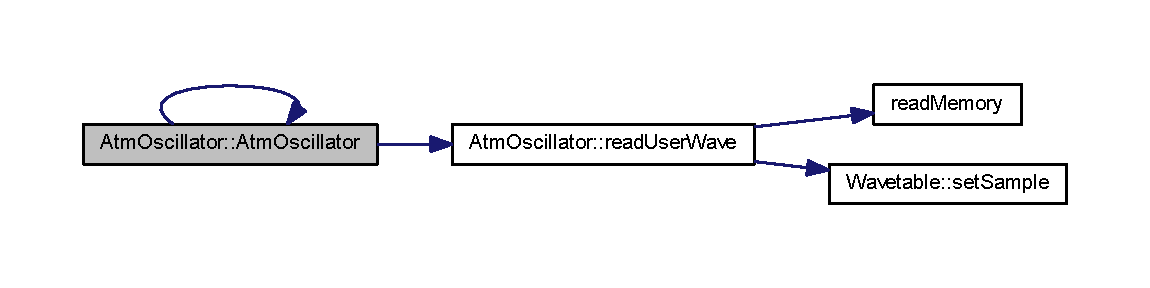
\includegraphics[width=350pt]{class_atm_oscillator_a864b35c83864a6d5045f9dbb42fa862e_cgraph}
\end{center}
\end{figure}
Here is the caller graph for this function\+:
\nopagebreak
\begin{figure}[H]
\begin{center}
\leavevmode
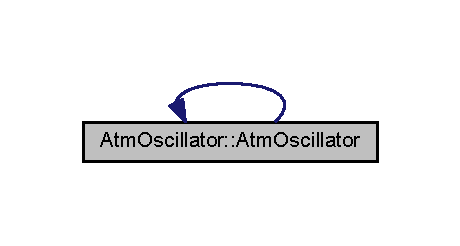
\includegraphics[width=221pt]{class_atm_oscillator_a864b35c83864a6d5045f9dbb42fa862e_icgraph}
\end{center}
\end{figure}
\mbox{\Hypertarget{class_atm_oscillator_a3d5b959eff3a2cb4fa3200cadeb2ab0b}\label{class_atm_oscillator_a3d5b959eff3a2cb4fa3200cadeb2ab0b}} 
\index{Atm\+Oscillator@{Atm\+Oscillator}!````~Atm\+Oscillator@{$\sim$\+Atm\+Oscillator}}
\index{````~Atm\+Oscillator@{$\sim$\+Atm\+Oscillator}!Atm\+Oscillator@{Atm\+Oscillator}}
\subsubsection{\texorpdfstring{$\sim$\+Atm\+Oscillator()}{~AtmOscillator()}}
{\footnotesize\ttfamily Atm\+Oscillator\+::$\sim$\+Atm\+Oscillator (\begin{DoxyParamCaption}{ }\end{DoxyParamCaption})}



Definition at line 32 of file Atm\+Oscillator.\+cpp.



\subsection{Member Function Documentation}
\mbox{\Hypertarget{class_atm_oscillator_ab0b1ab90e227ced30ddffff96bec6427}\label{class_atm_oscillator_ab0b1ab90e227ced30ddffff96bec6427}} 
\index{Atm\+Oscillator@{Atm\+Oscillator}!copy\+Wavetable@{copy\+Wavetable}}
\index{copy\+Wavetable@{copy\+Wavetable}!Atm\+Oscillator@{Atm\+Oscillator}}
\subsubsection{\texorpdfstring{copy\+Wavetable()}{copyWavetable()}}
{\footnotesize\ttfamily void Atm\+Oscillator\+::copy\+Wavetable (\begin{DoxyParamCaption}\item[{\hyperlink{class_wavetable}{Wavetable} \&}]{dest\+Wavetable }\end{DoxyParamCaption})}



Definition at line 40 of file Atm\+Oscillator.\+cpp.

Here is the call graph for this function\+:
\nopagebreak
\begin{figure}[H]
\begin{center}
\leavevmode
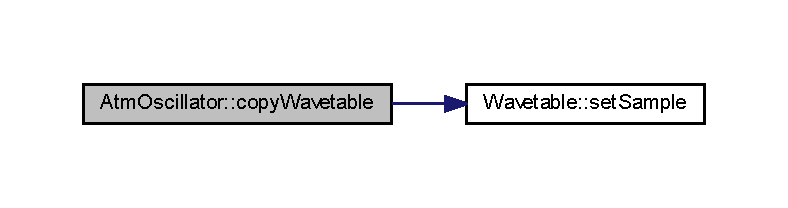
\includegraphics[width=350pt]{class_atm_oscillator_ab0b1ab90e227ced30ddffff96bec6427_cgraph}
\end{center}
\end{figure}
Here is the caller graph for this function\+:
\nopagebreak
\begin{figure}[H]
\begin{center}
\leavevmode
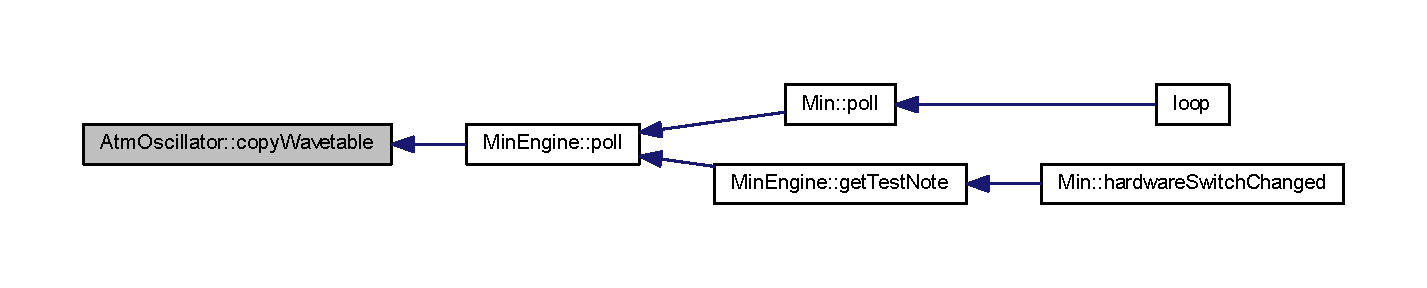
\includegraphics[width=350pt]{class_atm_oscillator_ab0b1ab90e227ced30ddffff96bec6427_icgraph}
\end{center}
\end{figure}
\mbox{\Hypertarget{class_atm_oscillator_a56b407e4175f4625e2e0d7a6f87c2225}\label{class_atm_oscillator_a56b407e4175f4625e2e0d7a6f87c2225}} 
\index{Atm\+Oscillator@{Atm\+Oscillator}!get\+Bank@{get\+Bank}}
\index{get\+Bank@{get\+Bank}!Atm\+Oscillator@{Atm\+Oscillator}}
\subsubsection{\texorpdfstring{get\+Bank()}{getBank()}}
{\footnotesize\ttfamily unsigned char Atm\+Oscillator\+::get\+Bank (\begin{DoxyParamCaption}{ }\end{DoxyParamCaption})\hspace{0.3cm}{\ttfamily [inline]}}



Definition at line 46 of file Atm\+Oscillator.\+h.

Here is the call graph for this function\+:
\nopagebreak
\begin{figure}[H]
\begin{center}
\leavevmode
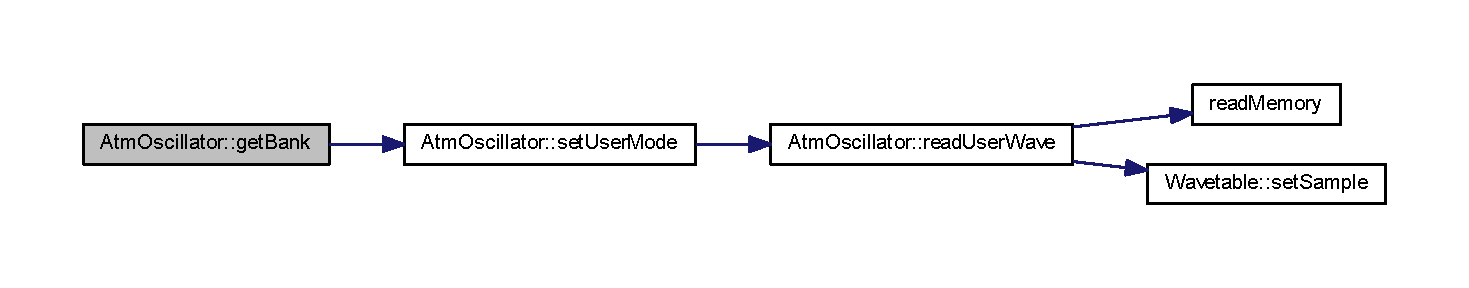
\includegraphics[width=350pt]{class_atm_oscillator_a56b407e4175f4625e2e0d7a6f87c2225_cgraph}
\end{center}
\end{figure}
\mbox{\Hypertarget{class_atm_oscillator_aa6fe7de8b2d573159271a47f5c8686e1}\label{class_atm_oscillator_aa6fe7de8b2d573159271a47f5c8686e1}} 
\index{Atm\+Oscillator@{Atm\+Oscillator}!get\+Sample@{get\+Sample}}
\index{get\+Sample@{get\+Sample}!Atm\+Oscillator@{Atm\+Oscillator}}
\subsubsection{\texorpdfstring{get\+Sample()}{getSample()}}
{\footnotesize\ttfamily char Atm\+Oscillator\+::get\+Sample (\begin{DoxyParamCaption}\item[{unsigned char}]{index }\end{DoxyParamCaption})}



Definition at line 68 of file Atm\+Oscillator.\+cpp.

Here is the caller graph for this function\+:
\nopagebreak
\begin{figure}[H]
\begin{center}
\leavevmode
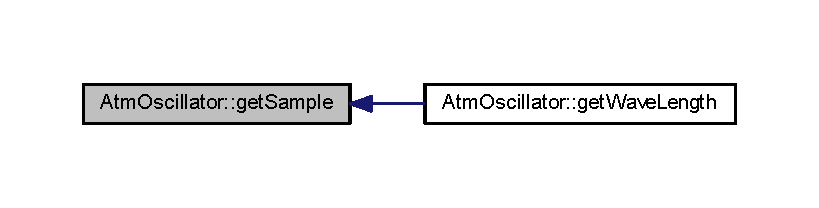
\includegraphics[width=350pt]{class_atm_oscillator_aa6fe7de8b2d573159271a47f5c8686e1_icgraph}
\end{center}
\end{figure}
\mbox{\Hypertarget{class_atm_oscillator_a01e9856e38a1e83b5d83fd503d5ad80e}\label{class_atm_oscillator_a01e9856e38a1e83b5d83fd503d5ad80e}} 
\index{Atm\+Oscillator@{Atm\+Oscillator}!get\+Table@{get\+Table}}
\index{get\+Table@{get\+Table}!Atm\+Oscillator@{Atm\+Oscillator}}
\subsubsection{\texorpdfstring{get\+Table()}{getTable()}}
{\footnotesize\ttfamily unsigned char Atm\+Oscillator\+::get\+Table (\begin{DoxyParamCaption}{ }\end{DoxyParamCaption})\hspace{0.3cm}{\ttfamily [inline]}}



Definition at line 44 of file Atm\+Oscillator.\+h.

\mbox{\Hypertarget{class_atm_oscillator_a21a4425606aa28eabf47a28ea7f02c9a}\label{class_atm_oscillator_a21a4425606aa28eabf47a28ea7f02c9a}} 
\index{Atm\+Oscillator@{Atm\+Oscillator}!get\+User\+Mode@{get\+User\+Mode}}
\index{get\+User\+Mode@{get\+User\+Mode}!Atm\+Oscillator@{Atm\+Oscillator}}
\subsubsection{\texorpdfstring{get\+User\+Mode()}{getUserMode()}}
{\footnotesize\ttfamily bool Atm\+Oscillator\+::get\+User\+Mode (\begin{DoxyParamCaption}{ }\end{DoxyParamCaption})\hspace{0.3cm}{\ttfamily [inline]}}



Definition at line 48 of file Atm\+Oscillator.\+h.

\mbox{\Hypertarget{class_atm_oscillator_a19bdaa400d57eeb24ca027febc2fd1cf}\label{class_atm_oscillator_a19bdaa400d57eeb24ca027febc2fd1cf}} 
\index{Atm\+Oscillator@{Atm\+Oscillator}!get\+User\+Wave\+Start\+Address@{get\+User\+Wave\+Start\+Address}}
\index{get\+User\+Wave\+Start\+Address@{get\+User\+Wave\+Start\+Address}!Atm\+Oscillator@{Atm\+Oscillator}}
\subsubsection{\texorpdfstring{get\+User\+Wave\+Start\+Address()}{getUserWaveStartAddress()}}
{\footnotesize\ttfamily unsigned int Atm\+Oscillator\+::get\+User\+Wave\+Start\+Address (\begin{DoxyParamCaption}{ }\end{DoxyParamCaption})\hspace{0.3cm}{\ttfamily [inline]}}



Definition at line 53 of file Atm\+Oscillator.\+h.

Here is the call graph for this function\+:
\nopagebreak
\begin{figure}[H]
\begin{center}
\leavevmode
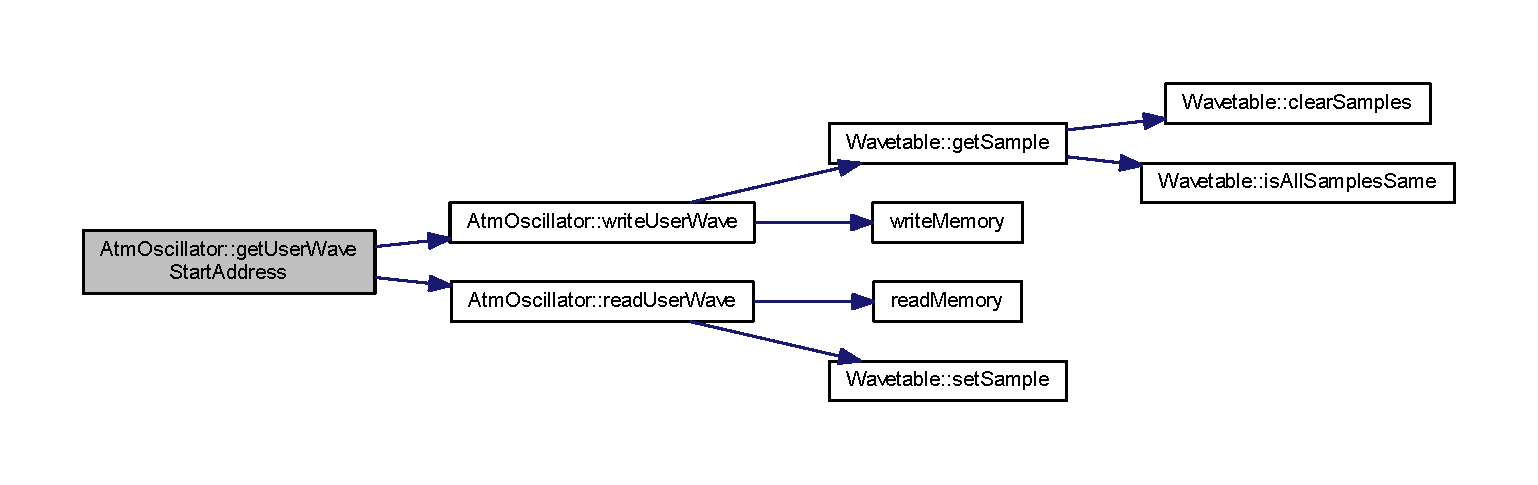
\includegraphics[width=350pt]{class_atm_oscillator_a19bdaa400d57eeb24ca027febc2fd1cf_cgraph}
\end{center}
\end{figure}
\mbox{\Hypertarget{class_atm_oscillator_ae5ef1556ef77dbf9ecceb5b64a1ad7e8}\label{class_atm_oscillator_ae5ef1556ef77dbf9ecceb5b64a1ad7e8}} 
\index{Atm\+Oscillator@{Atm\+Oscillator}!get\+User\+Wavetable\+Sample@{get\+User\+Wavetable\+Sample}}
\index{get\+User\+Wavetable\+Sample@{get\+User\+Wavetable\+Sample}!Atm\+Oscillator@{Atm\+Oscillator}}
\subsubsection{\texorpdfstring{get\+User\+Wavetable\+Sample()}{getUserWavetableSample()}}
{\footnotesize\ttfamily char Atm\+Oscillator\+::get\+User\+Wavetable\+Sample (\begin{DoxyParamCaption}\item[{unsigned char}]{index }\end{DoxyParamCaption})}



Definition at line 99 of file Atm\+Oscillator.\+cpp.

Here is the call graph for this function\+:
\nopagebreak
\begin{figure}[H]
\begin{center}
\leavevmode
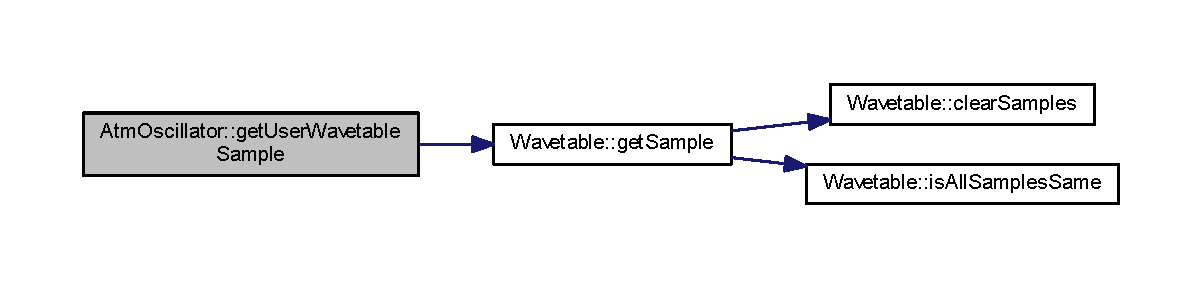
\includegraphics[width=350pt]{class_atm_oscillator_ae5ef1556ef77dbf9ecceb5b64a1ad7e8_cgraph}
\end{center}
\end{figure}
Here is the caller graph for this function\+:
\nopagebreak
\begin{figure}[H]
\begin{center}
\leavevmode
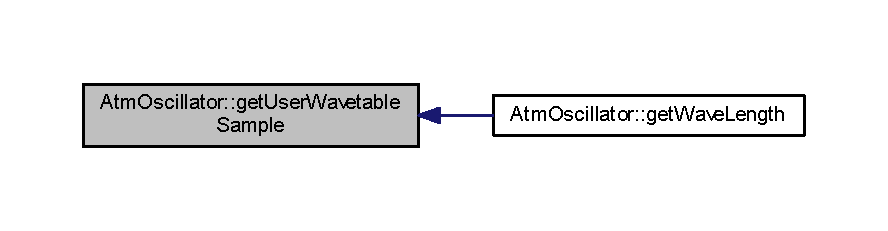
\includegraphics[width=350pt]{class_atm_oscillator_ae5ef1556ef77dbf9ecceb5b64a1ad7e8_icgraph}
\end{center}
\end{figure}
\mbox{\Hypertarget{class_atm_oscillator_ad846116dfd6f232cae79ada35dddadfd}\label{class_atm_oscillator_ad846116dfd6f232cae79ada35dddadfd}} 
\index{Atm\+Oscillator@{Atm\+Oscillator}!get\+Wave\+Length@{get\+Wave\+Length}}
\index{get\+Wave\+Length@{get\+Wave\+Length}!Atm\+Oscillator@{Atm\+Oscillator}}
\subsubsection{\texorpdfstring{get\+Wave\+Length()}{getWaveLength()}}
{\footnotesize\ttfamily unsigned char Atm\+Oscillator\+::get\+Wave\+Length (\begin{DoxyParamCaption}{ }\end{DoxyParamCaption})\hspace{0.3cm}{\ttfamily [inline]}}



Definition at line 49 of file Atm\+Oscillator.\+h.

Here is the call graph for this function\+:
\nopagebreak
\begin{figure}[H]
\begin{center}
\leavevmode
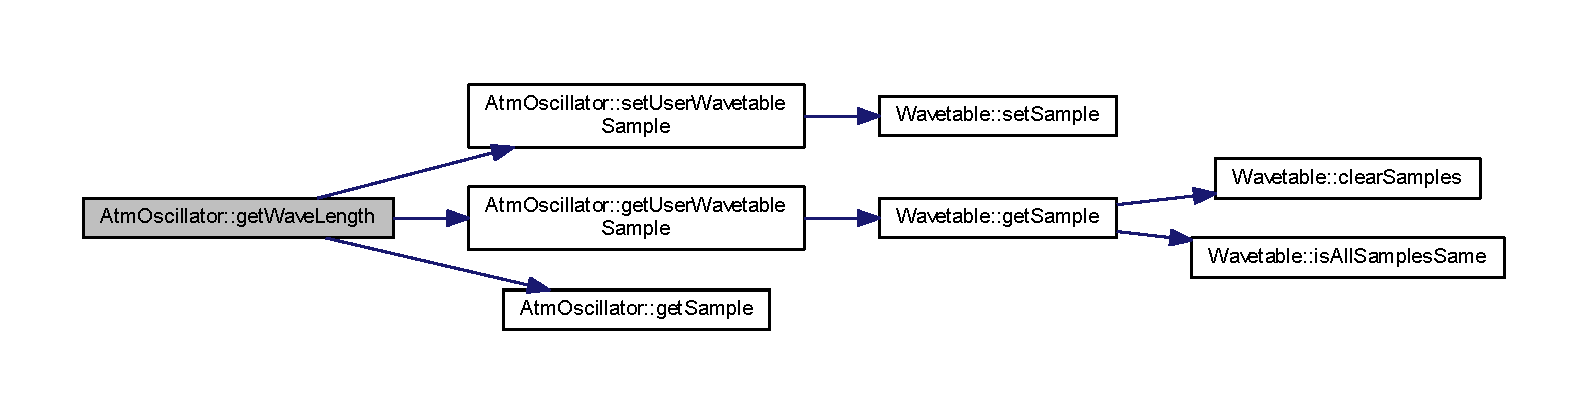
\includegraphics[width=350pt]{class_atm_oscillator_ad846116dfd6f232cae79ada35dddadfd_cgraph}
\end{center}
\end{figure}
\mbox{\Hypertarget{class_atm_oscillator_a08b383cd2305c232de827399aa8d2ccb}\label{class_atm_oscillator_a08b383cd2305c232de827399aa8d2ccb}} 
\index{Atm\+Oscillator@{Atm\+Oscillator}!read\+User\+Wave@{read\+User\+Wave}}
\index{read\+User\+Wave@{read\+User\+Wave}!Atm\+Oscillator@{Atm\+Oscillator}}
\subsubsection{\texorpdfstring{read\+User\+Wave()}{readUserWave()}}
{\footnotesize\ttfamily void Atm\+Oscillator\+::read\+User\+Wave (\begin{DoxyParamCaption}\item[{unsigned char}]{wave\+Num }\end{DoxyParamCaption})}



Definition at line 113 of file Atm\+Oscillator.\+cpp.

Here is the call graph for this function\+:
\nopagebreak
\begin{figure}[H]
\begin{center}
\leavevmode
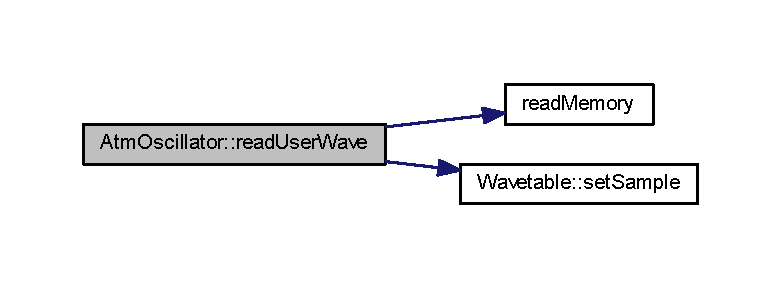
\includegraphics[width=350pt]{class_atm_oscillator_a08b383cd2305c232de827399aa8d2ccb_cgraph}
\end{center}
\end{figure}
Here is the caller graph for this function\+:
\nopagebreak
\begin{figure}[H]
\begin{center}
\leavevmode
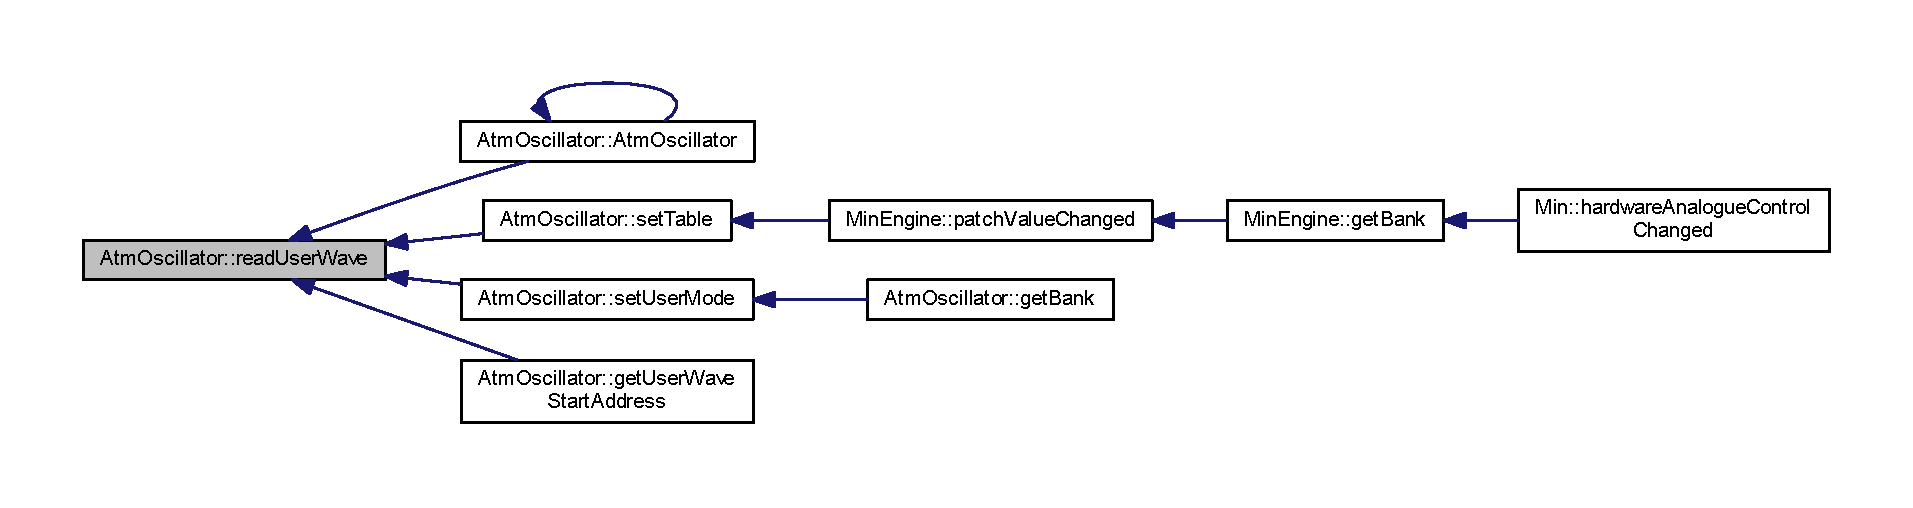
\includegraphics[width=350pt]{class_atm_oscillator_a08b383cd2305c232de827399aa8d2ccb_icgraph}
\end{center}
\end{figure}
\mbox{\Hypertarget{class_atm_oscillator_a9f65ae9f2132c46f73b776a869b5bf21}\label{class_atm_oscillator_a9f65ae9f2132c46f73b776a869b5bf21}} 
\index{Atm\+Oscillator@{Atm\+Oscillator}!set\+Bank@{set\+Bank}}
\index{set\+Bank@{set\+Bank}!Atm\+Oscillator@{Atm\+Oscillator}}
\subsubsection{\texorpdfstring{set\+Bank()}{setBank()}}
{\footnotesize\ttfamily void Atm\+Oscillator\+::set\+Bank (\begin{DoxyParamCaption}\item[{unsigned char}]{new\+Bank }\end{DoxyParamCaption})\hspace{0.3cm}{\ttfamily [inline]}}



Definition at line 45 of file Atm\+Oscillator.\+h.

Here is the caller graph for this function\+:
\nopagebreak
\begin{figure}[H]
\begin{center}
\leavevmode
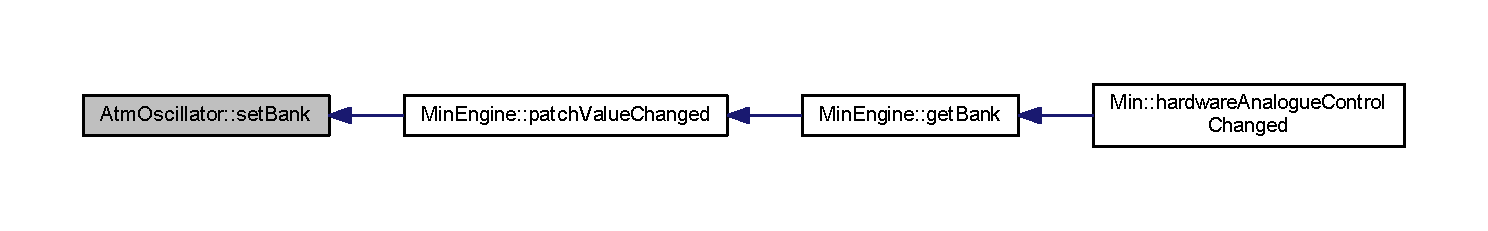
\includegraphics[width=350pt]{class_atm_oscillator_a9f65ae9f2132c46f73b776a869b5bf21_icgraph}
\end{center}
\end{figure}
\mbox{\Hypertarget{class_atm_oscillator_ac4248a3cd6fceea6ee677e74faba4af0}\label{class_atm_oscillator_ac4248a3cd6fceea6ee677e74faba4af0}} 
\index{Atm\+Oscillator@{Atm\+Oscillator}!set\+Table@{set\+Table}}
\index{set\+Table@{set\+Table}!Atm\+Oscillator@{Atm\+Oscillator}}
\subsubsection{\texorpdfstring{set\+Table()}{setTable()}}
{\footnotesize\ttfamily void Atm\+Oscillator\+::set\+Table (\begin{DoxyParamCaption}\item[{unsigned char}]{new\+Table }\end{DoxyParamCaption})}



Definition at line 79 of file Atm\+Oscillator.\+cpp.

Here is the call graph for this function\+:
\nopagebreak
\begin{figure}[H]
\begin{center}
\leavevmode
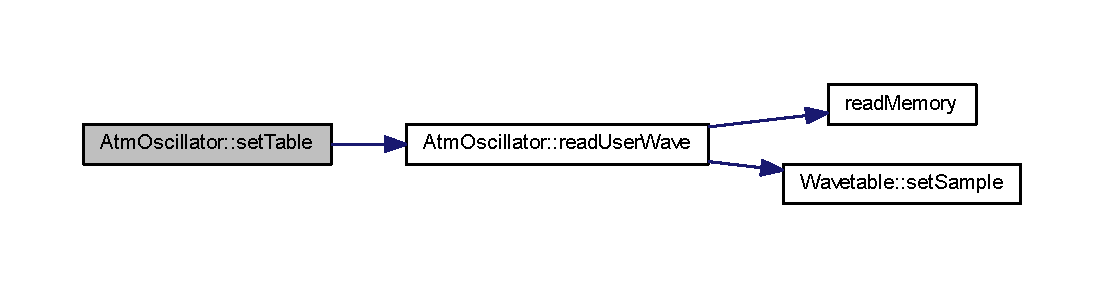
\includegraphics[width=350pt]{class_atm_oscillator_ac4248a3cd6fceea6ee677e74faba4af0_cgraph}
\end{center}
\end{figure}
Here is the caller graph for this function\+:
\nopagebreak
\begin{figure}[H]
\begin{center}
\leavevmode
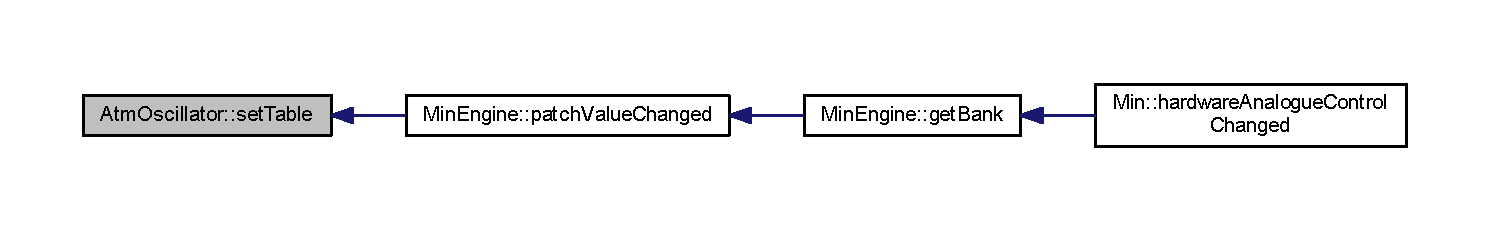
\includegraphics[width=350pt]{class_atm_oscillator_ac4248a3cd6fceea6ee677e74faba4af0_icgraph}
\end{center}
\end{figure}
\mbox{\Hypertarget{class_atm_oscillator_aafaccbb54d52f2c0eb07eb968498eef4}\label{class_atm_oscillator_aafaccbb54d52f2c0eb07eb968498eef4}} 
\index{Atm\+Oscillator@{Atm\+Oscillator}!set\+User\+Mode@{set\+User\+Mode}}
\index{set\+User\+Mode@{set\+User\+Mode}!Atm\+Oscillator@{Atm\+Oscillator}}
\subsubsection{\texorpdfstring{set\+User\+Mode()}{setUserMode()}}
{\footnotesize\ttfamily void Atm\+Oscillator\+::set\+User\+Mode (\begin{DoxyParamCaption}\item[{bool}]{new\+User\+Mode }\end{DoxyParamCaption})}



Definition at line 87 of file Atm\+Oscillator.\+cpp.

Here is the call graph for this function\+:
\nopagebreak
\begin{figure}[H]
\begin{center}
\leavevmode
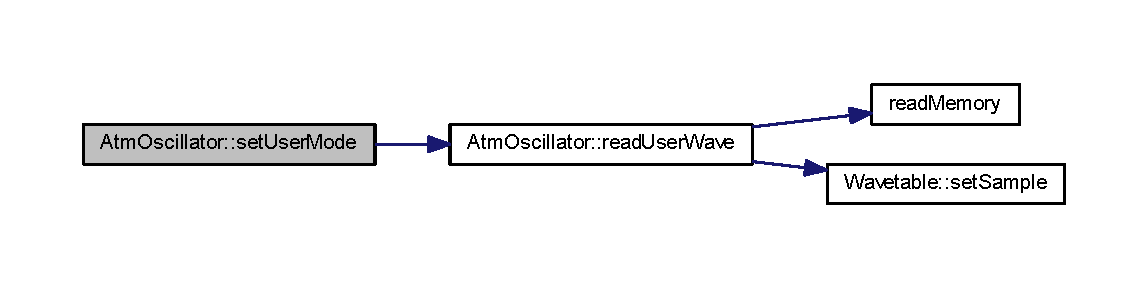
\includegraphics[width=350pt]{class_atm_oscillator_aafaccbb54d52f2c0eb07eb968498eef4_cgraph}
\end{center}
\end{figure}
Here is the caller graph for this function\+:
\nopagebreak
\begin{figure}[H]
\begin{center}
\leavevmode
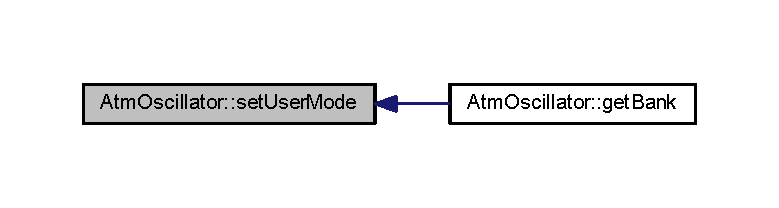
\includegraphics[width=350pt]{class_atm_oscillator_aafaccbb54d52f2c0eb07eb968498eef4_icgraph}
\end{center}
\end{figure}
\mbox{\Hypertarget{class_atm_oscillator_aa62dba14693f65adcb3daa7aa4757ba1}\label{class_atm_oscillator_aa62dba14693f65adcb3daa7aa4757ba1}} 
\index{Atm\+Oscillator@{Atm\+Oscillator}!set\+User\+Wavetable\+Sample@{set\+User\+Wavetable\+Sample}}
\index{set\+User\+Wavetable\+Sample@{set\+User\+Wavetable\+Sample}!Atm\+Oscillator@{Atm\+Oscillator}}
\subsubsection{\texorpdfstring{set\+User\+Wavetable\+Sample()}{setUserWavetableSample()}}
{\footnotesize\ttfamily void Atm\+Oscillator\+::set\+User\+Wavetable\+Sample (\begin{DoxyParamCaption}\item[{unsigned char}]{index,  }\item[{char}]{new\+Sample }\end{DoxyParamCaption})}



Definition at line 95 of file Atm\+Oscillator.\+cpp.

Here is the call graph for this function\+:
\nopagebreak
\begin{figure}[H]
\begin{center}
\leavevmode
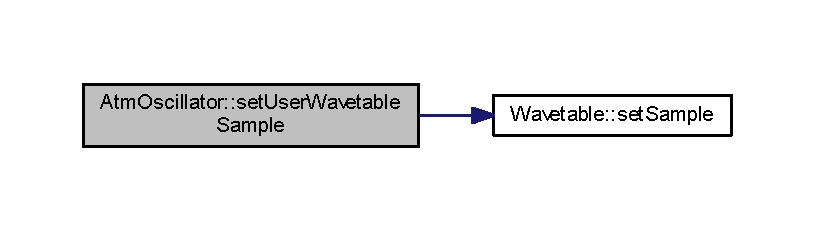
\includegraphics[width=350pt]{class_atm_oscillator_aa62dba14693f65adcb3daa7aa4757ba1_cgraph}
\end{center}
\end{figure}
Here is the caller graph for this function\+:
\nopagebreak
\begin{figure}[H]
\begin{center}
\leavevmode
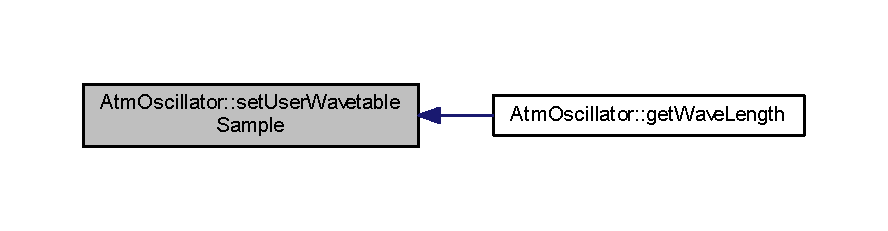
\includegraphics[width=350pt]{class_atm_oscillator_aa62dba14693f65adcb3daa7aa4757ba1_icgraph}
\end{center}
\end{figure}
\mbox{\Hypertarget{class_atm_oscillator_a92133ff9c3b34a6acb703f0d6d95cd71}\label{class_atm_oscillator_a92133ff9c3b34a6acb703f0d6d95cd71}} 
\index{Atm\+Oscillator@{Atm\+Oscillator}!write\+User\+Wave@{write\+User\+Wave}}
\index{write\+User\+Wave@{write\+User\+Wave}!Atm\+Oscillator@{Atm\+Oscillator}}
\subsubsection{\texorpdfstring{write\+User\+Wave()}{writeUserWave()}}
{\footnotesize\ttfamily void Atm\+Oscillator\+::write\+User\+Wave (\begin{DoxyParamCaption}\item[{unsigned char}]{wave\+Num }\end{DoxyParamCaption})}



Definition at line 103 of file Atm\+Oscillator.\+cpp.

Here is the call graph for this function\+:
\nopagebreak
\begin{figure}[H]
\begin{center}
\leavevmode
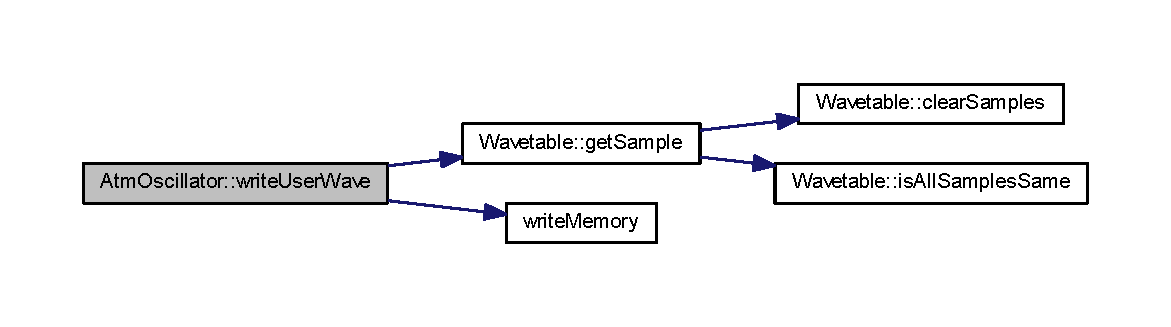
\includegraphics[width=350pt]{class_atm_oscillator_a92133ff9c3b34a6acb703f0d6d95cd71_cgraph}
\end{center}
\end{figure}
Here is the caller graph for this function\+:
\nopagebreak
\begin{figure}[H]
\begin{center}
\leavevmode
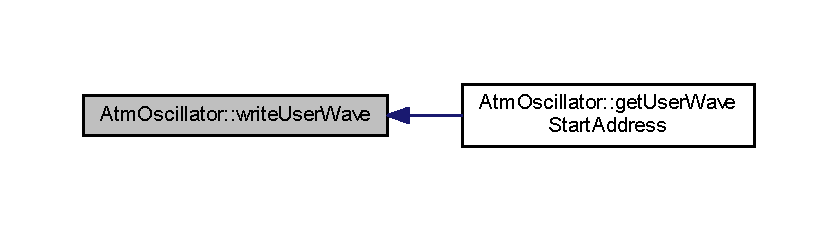
\includegraphics[width=350pt]{class_atm_oscillator_a92133ff9c3b34a6acb703f0d6d95cd71_icgraph}
\end{center}
\end{figure}


The documentation for this class was generated from the following files\+:\begin{DoxyCompactItemize}
\item 
\hyperlink{_atm_oscillator_8h}{Atm\+Oscillator.\+h}\item 
\hyperlink{_atm_oscillator_8cpp}{Atm\+Oscillator.\+cpp}\end{DoxyCompactItemize}

\hypertarget{class_atm_patch}{}\section{Atm\+Patch Class Reference}
\label{class_atm_patch}\index{Atm\+Patch@{Atm\+Patch}}


{\ttfamily \#include \char`\"{}Atm\+Patch.\+h\char`\"{}}



Collaboration diagram for Atm\+Patch\+:
\nopagebreak
\begin{figure}[H]
\begin{center}
\leavevmode
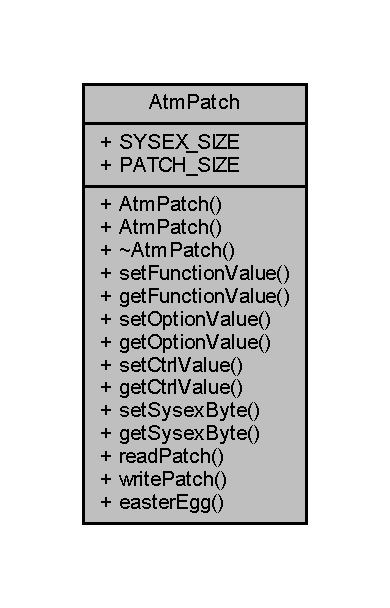
\includegraphics[width=187pt]{d5/d25/class_atm_patch__coll__graph}
\end{center}
\end{figure}
\subsection*{Public Member Functions}
\begin{DoxyCompactItemize}
\item 
\hyperlink{class_atm_patch_ad9b5a85c314ca968deae87ca43b087e9}{Atm\+Patch} (\hyperlink{class_atm_patch_base}{Atm\+Patch\+Base} $\ast$base)
\item 
\hyperlink{class_atm_patch_ac9d24dbe3f01ee12145649819017f697}{Atm\+Patch} ()
\item 
\hyperlink{class_atm_patch_ae37c93d358677907afbcc74c34469ba2}{$\sim$\+Atm\+Patch} ()
\item 
void \hyperlink{class_atm_patch_ad2fe7a265755afc95a36752b86b6a7e2}{set\+Function\+Value} (unsigned char func, unsigned char new\+Value)
\item 
unsigned char \hyperlink{class_atm_patch_a7b4184a7f5bd314e150f9ad38cc3a0fb}{get\+Function\+Value} (unsigned char func)
\item 
void \hyperlink{class_atm_patch_a1139606bcbffe63881b3f175f577d8e1}{set\+Option\+Value} (unsigned char func, bool new\+Value)
\item 
bool \hyperlink{class_atm_patch_ab521c0a108bf7f8bc848755c38330bc0}{get\+Option\+Value} (unsigned char func)
\item 
void \hyperlink{class_atm_patch_a95fb3ea0dfd3369abe7518da26edb1b5}{set\+Ctrl\+Value} (unsigned char bank, unsigned char ctrl, unsigned char new\+Value)
\item 
unsigned char \hyperlink{class_atm_patch_a5e8835fb80bdd1f130f129edde447d35}{get\+Ctrl\+Value} (unsigned char bank, unsigned char ctrl)
\item 
void \hyperlink{class_atm_patch_acc2729c3b10aa4d7f98e67caa3b80255}{set\+Sysex\+Byte} (unsigned char index, unsigned char new\+Value)
\item 
unsigned char \hyperlink{class_atm_patch_a48b5b2d71e4b83b80979a68372e935ae}{get\+Sysex\+Byte} (unsigned char index)
\item 
void \hyperlink{class_atm_patch_a9689db39f28d3c7d0fcaa6966c82e2d6}{read\+Patch} (unsigned char patch\+Num)
\item 
void \hyperlink{class_atm_patch_a5814cd528970cb153dd67865a6b86c85}{write\+Patch} (unsigned char patch\+Num)
\item 
void \hyperlink{class_atm_patch_ad7a325c544381189f9419131feba685b}{easter\+Egg} (unsigned int seed)
\end{DoxyCompactItemize}
\subsection*{Static Public Attributes}
\begin{DoxyCompactItemize}
\item 
static const unsigned char \hyperlink{class_atm_patch_a042c0c97fac54f61b229ad08e71037cb}{S\+Y\+S\+E\+X\+\_\+\+S\+I\+ZE} = 44
\item 
static const unsigned char \hyperlink{class_atm_patch_a1ae078abd4f165fa8b0eb14d0acd48c0}{P\+A\+T\+C\+H\+\_\+\+S\+I\+ZE} = 22
\end{DoxyCompactItemize}


\subsection{Detailed Description}


Definition at line 44 of file Atm\+Patch.\+h.



\subsection{Constructor \& Destructor Documentation}
\mbox{\Hypertarget{class_atm_patch_ad9b5a85c314ca968deae87ca43b087e9}\label{class_atm_patch_ad9b5a85c314ca968deae87ca43b087e9}} 
\index{Atm\+Patch@{Atm\+Patch}!Atm\+Patch@{Atm\+Patch}}
\index{Atm\+Patch@{Atm\+Patch}!Atm\+Patch@{Atm\+Patch}}
\subsubsection{\texorpdfstring{Atm\+Patch()}{AtmPatch()}\hspace{0.1cm}{\footnotesize\ttfamily [1/2]}}
{\footnotesize\ttfamily Atm\+Patch\+::\+Atm\+Patch (\begin{DoxyParamCaption}\item[{\hyperlink{class_atm_patch_base}{Atm\+Patch\+Base} $\ast$}]{base }\end{DoxyParamCaption})}



Definition at line 22 of file Atm\+Patch.\+cpp.

\mbox{\Hypertarget{class_atm_patch_ac9d24dbe3f01ee12145649819017f697}\label{class_atm_patch_ac9d24dbe3f01ee12145649819017f697}} 
\index{Atm\+Patch@{Atm\+Patch}!Atm\+Patch@{Atm\+Patch}}
\index{Atm\+Patch@{Atm\+Patch}!Atm\+Patch@{Atm\+Patch}}
\subsubsection{\texorpdfstring{Atm\+Patch()}{AtmPatch()}\hspace{0.1cm}{\footnotesize\ttfamily [2/2]}}
{\footnotesize\ttfamily Atm\+Patch\+::\+Atm\+Patch (\begin{DoxyParamCaption}{ }\end{DoxyParamCaption})\hspace{0.3cm}{\ttfamily [inline]}}



Definition at line 65 of file Atm\+Patch.\+h.

Here is the call graph for this function\+:
\nopagebreak
\begin{figure}[H]
\begin{center}
\leavevmode
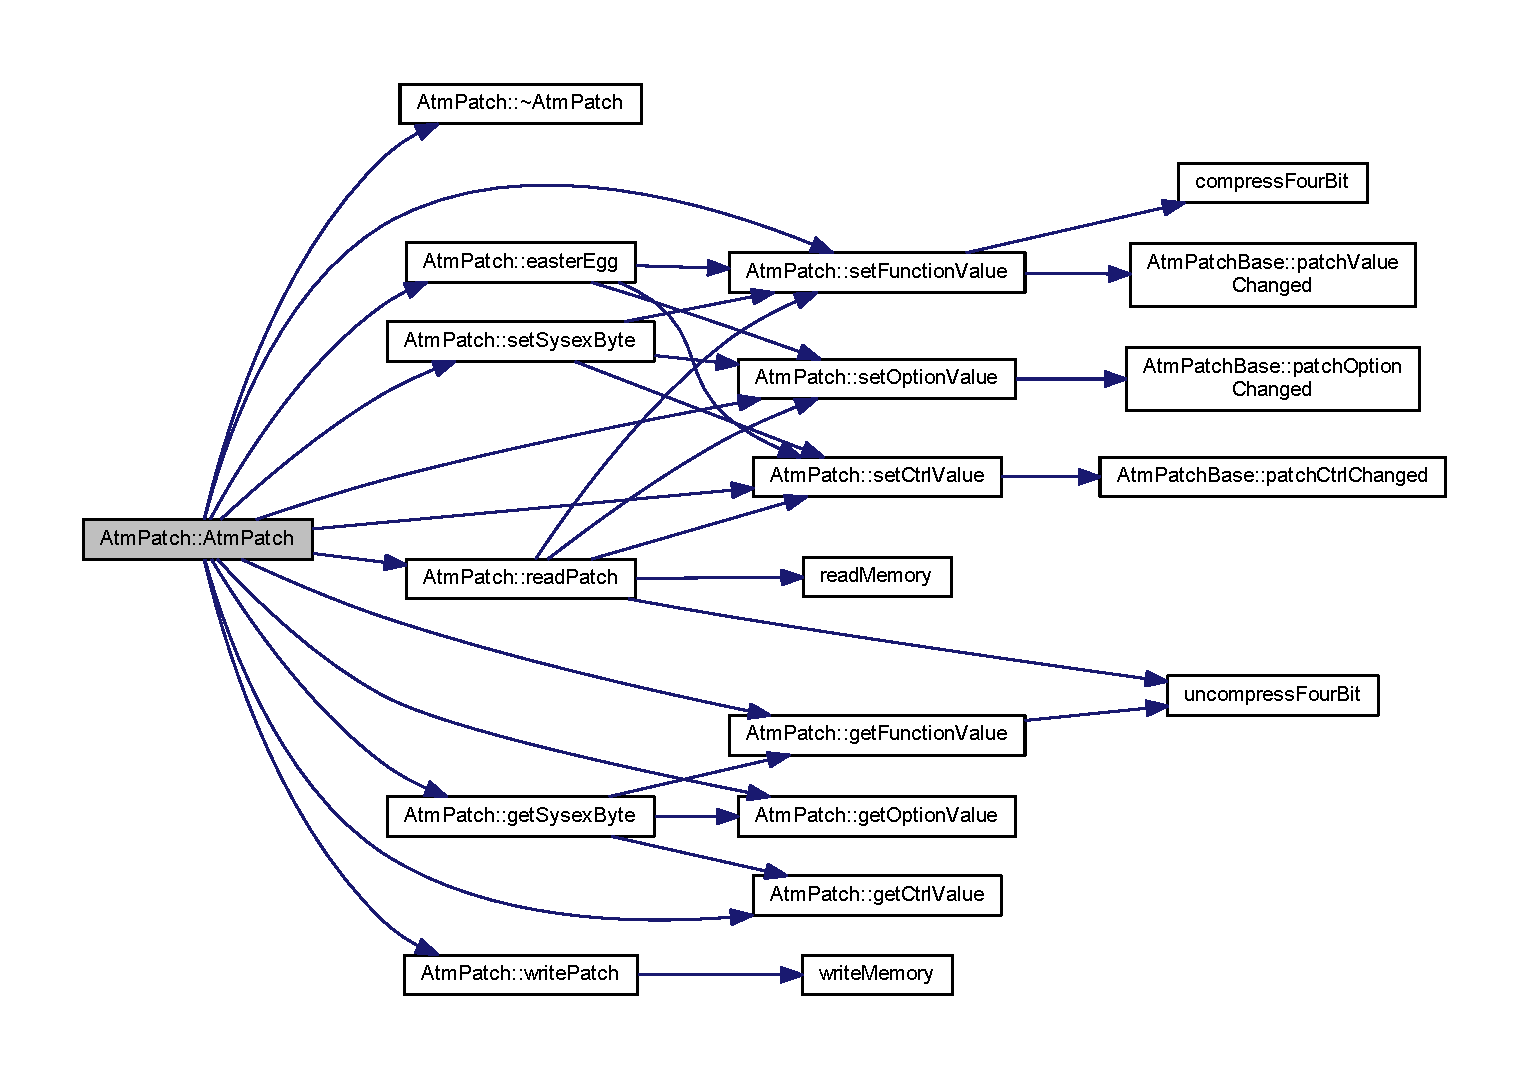
\includegraphics[width=350pt]{d9/de1/class_atm_patch_ac9d24dbe3f01ee12145649819017f697_cgraph}
\end{center}
\end{figure}
\mbox{\Hypertarget{class_atm_patch_ae37c93d358677907afbcc74c34469ba2}\label{class_atm_patch_ae37c93d358677907afbcc74c34469ba2}} 
\index{Atm\+Patch@{Atm\+Patch}!````~Atm\+Patch@{$\sim$\+Atm\+Patch}}
\index{````~Atm\+Patch@{$\sim$\+Atm\+Patch}!Atm\+Patch@{Atm\+Patch}}
\subsubsection{\texorpdfstring{$\sim$\+Atm\+Patch()}{~AtmPatch()}}
{\footnotesize\ttfamily Atm\+Patch\+::$\sim$\+Atm\+Patch (\begin{DoxyParamCaption}{ }\end{DoxyParamCaption})}



Definition at line 31 of file Atm\+Patch.\+cpp.

Here is the caller graph for this function\+:
\nopagebreak
\begin{figure}[H]
\begin{center}
\leavevmode
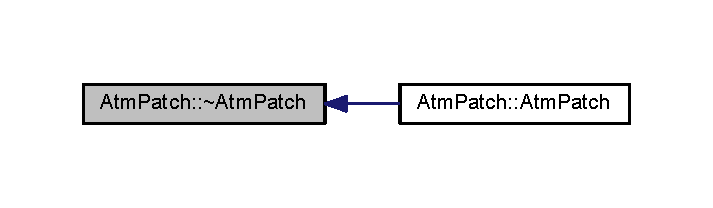
\includegraphics[width=342pt]{d9/de1/class_atm_patch_ae37c93d358677907afbcc74c34469ba2_icgraph}
\end{center}
\end{figure}


\subsection{Member Function Documentation}
\mbox{\Hypertarget{class_atm_patch_ad7a325c544381189f9419131feba685b}\label{class_atm_patch_ad7a325c544381189f9419131feba685b}} 
\index{Atm\+Patch@{Atm\+Patch}!easter\+Egg@{easter\+Egg}}
\index{easter\+Egg@{easter\+Egg}!Atm\+Patch@{Atm\+Patch}}
\subsubsection{\texorpdfstring{easter\+Egg()}{easterEgg()}}
{\footnotesize\ttfamily void Atm\+Patch\+::easter\+Egg (\begin{DoxyParamCaption}\item[{unsigned int}]{seed }\end{DoxyParamCaption})}



Definition at line 176 of file Atm\+Patch.\+cpp.

Here is the call graph for this function\+:
\nopagebreak
\begin{figure}[H]
\begin{center}
\leavevmode
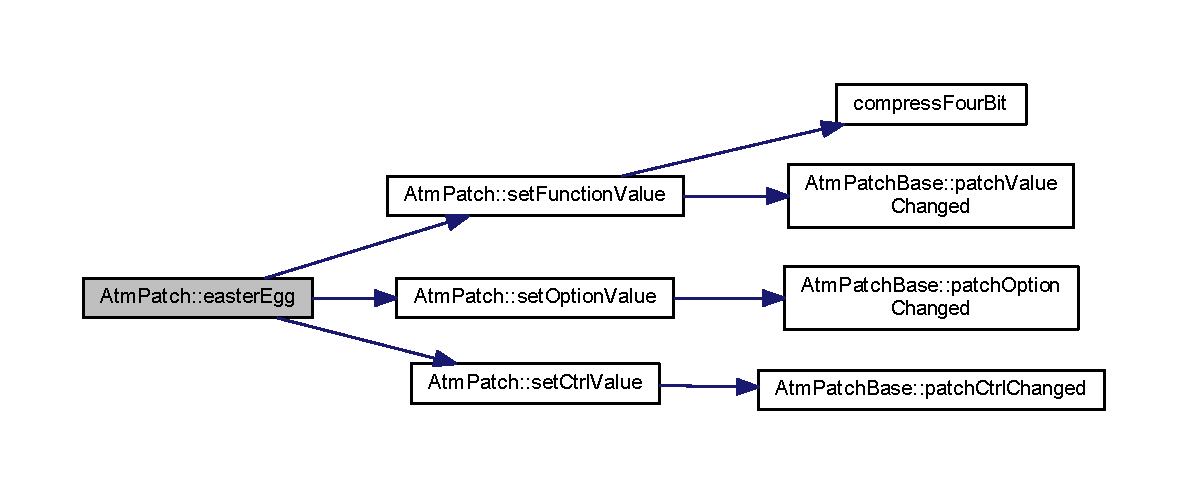
\includegraphics[width=350pt]{d9/de1/class_atm_patch_ad7a325c544381189f9419131feba685b_cgraph}
\end{center}
\end{figure}
Here is the caller graph for this function\+:
\nopagebreak
\begin{figure}[H]
\begin{center}
\leavevmode
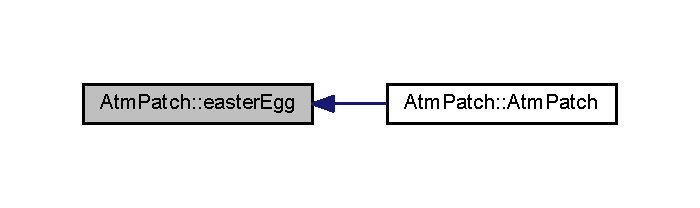
\includegraphics[width=336pt]{d9/de1/class_atm_patch_ad7a325c544381189f9419131feba685b_icgraph}
\end{center}
\end{figure}
\mbox{\Hypertarget{class_atm_patch_a5e8835fb80bdd1f130f129edde447d35}\label{class_atm_patch_a5e8835fb80bdd1f130f129edde447d35}} 
\index{Atm\+Patch@{Atm\+Patch}!get\+Ctrl\+Value@{get\+Ctrl\+Value}}
\index{get\+Ctrl\+Value@{get\+Ctrl\+Value}!Atm\+Patch@{Atm\+Patch}}
\subsubsection{\texorpdfstring{get\+Ctrl\+Value()}{getCtrlValue()}}
{\footnotesize\ttfamily unsigned char Atm\+Patch\+::get\+Ctrl\+Value (\begin{DoxyParamCaption}\item[{unsigned char}]{bank,  }\item[{unsigned char}]{ctrl }\end{DoxyParamCaption})}



Definition at line 78 of file Atm\+Patch.\+cpp.

Here is the caller graph for this function\+:
\nopagebreak
\begin{figure}[H]
\begin{center}
\leavevmode
\includegraphics[width=350pt]{d9/de1/class_atm_patch_a5e8835fb80bdd1f130f129edde447d35_icgraph}
\end{center}
\end{figure}
\mbox{\Hypertarget{class_atm_patch_a7b4184a7f5bd314e150f9ad38cc3a0fb}\label{class_atm_patch_a7b4184a7f5bd314e150f9ad38cc3a0fb}} 
\index{Atm\+Patch@{Atm\+Patch}!get\+Function\+Value@{get\+Function\+Value}}
\index{get\+Function\+Value@{get\+Function\+Value}!Atm\+Patch@{Atm\+Patch}}
\subsubsection{\texorpdfstring{get\+Function\+Value()}{getFunctionValue()}}
{\footnotesize\ttfamily unsigned char Atm\+Patch\+::get\+Function\+Value (\begin{DoxyParamCaption}\item[{unsigned char}]{func }\end{DoxyParamCaption})}



Definition at line 49 of file Atm\+Patch.\+cpp.

Here is the call graph for this function\+:
\nopagebreak
\begin{figure}[H]
\begin{center}
\leavevmode
\includegraphics[width=350pt]{d9/de1/class_atm_patch_a7b4184a7f5bd314e150f9ad38cc3a0fb_cgraph}
\end{center}
\end{figure}
Here is the caller graph for this function\+:
\nopagebreak
\begin{figure}[H]
\begin{center}
\leavevmode
\includegraphics[width=350pt]{d9/de1/class_atm_patch_a7b4184a7f5bd314e150f9ad38cc3a0fb_icgraph}
\end{center}
\end{figure}
\mbox{\Hypertarget{class_atm_patch_ab521c0a108bf7f8bc848755c38330bc0}\label{class_atm_patch_ab521c0a108bf7f8bc848755c38330bc0}} 
\index{Atm\+Patch@{Atm\+Patch}!get\+Option\+Value@{get\+Option\+Value}}
\index{get\+Option\+Value@{get\+Option\+Value}!Atm\+Patch@{Atm\+Patch}}
\subsubsection{\texorpdfstring{get\+Option\+Value()}{getOptionValue()}}
{\footnotesize\ttfamily bool Atm\+Patch\+::get\+Option\+Value (\begin{DoxyParamCaption}\item[{unsigned char}]{func }\end{DoxyParamCaption})}



Definition at line 64 of file Atm\+Patch.\+cpp.

Here is the caller graph for this function\+:
\nopagebreak
\begin{figure}[H]
\begin{center}
\leavevmode
\includegraphics[width=350pt]{d9/de1/class_atm_patch_ab521c0a108bf7f8bc848755c38330bc0_icgraph}
\end{center}
\end{figure}
\mbox{\Hypertarget{class_atm_patch_a48b5b2d71e4b83b80979a68372e935ae}\label{class_atm_patch_a48b5b2d71e4b83b80979a68372e935ae}} 
\index{Atm\+Patch@{Atm\+Patch}!get\+Sysex\+Byte@{get\+Sysex\+Byte}}
\index{get\+Sysex\+Byte@{get\+Sysex\+Byte}!Atm\+Patch@{Atm\+Patch}}
\subsubsection{\texorpdfstring{get\+Sysex\+Byte()}{getSysexByte()}}
{\footnotesize\ttfamily unsigned char Atm\+Patch\+::get\+Sysex\+Byte (\begin{DoxyParamCaption}\item[{unsigned char}]{index }\end{DoxyParamCaption})}



Definition at line 138 of file Atm\+Patch.\+cpp.

Here is the call graph for this function\+:
\nopagebreak
\begin{figure}[H]
\begin{center}
\leavevmode
\includegraphics[width=350pt]{d9/de1/class_atm_patch_a48b5b2d71e4b83b80979a68372e935ae_cgraph}
\end{center}
\end{figure}
Here is the caller graph for this function\+:
\nopagebreak
\begin{figure}[H]
\begin{center}
\leavevmode
\includegraphics[width=350pt]{d9/de1/class_atm_patch_a48b5b2d71e4b83b80979a68372e935ae_icgraph}
\end{center}
\end{figure}
\mbox{\Hypertarget{class_atm_patch_a9689db39f28d3c7d0fcaa6966c82e2d6}\label{class_atm_patch_a9689db39f28d3c7d0fcaa6966c82e2d6}} 
\index{Atm\+Patch@{Atm\+Patch}!read\+Patch@{read\+Patch}}
\index{read\+Patch@{read\+Patch}!Atm\+Patch@{Atm\+Patch}}
\subsubsection{\texorpdfstring{read\+Patch()}{readPatch()}}
{\footnotesize\ttfamily void Atm\+Patch\+::read\+Patch (\begin{DoxyParamCaption}\item[{unsigned char}]{patch\+Num }\end{DoxyParamCaption})}



Definition at line 108 of file Atm\+Patch.\+cpp.

Here is the call graph for this function\+:
\nopagebreak
\begin{figure}[H]
\begin{center}
\leavevmode
\includegraphics[width=350pt]{d9/de1/class_atm_patch_a9689db39f28d3c7d0fcaa6966c82e2d6_cgraph}
\end{center}
\end{figure}
Here is the caller graph for this function\+:
\nopagebreak
\begin{figure}[H]
\begin{center}
\leavevmode
\includegraphics[width=350pt]{d9/de1/class_atm_patch_a9689db39f28d3c7d0fcaa6966c82e2d6_icgraph}
\end{center}
\end{figure}
\mbox{\Hypertarget{class_atm_patch_a95fb3ea0dfd3369abe7518da26edb1b5}\label{class_atm_patch_a95fb3ea0dfd3369abe7518da26edb1b5}} 
\index{Atm\+Patch@{Atm\+Patch}!set\+Ctrl\+Value@{set\+Ctrl\+Value}}
\index{set\+Ctrl\+Value@{set\+Ctrl\+Value}!Atm\+Patch@{Atm\+Patch}}
\subsubsection{\texorpdfstring{set\+Ctrl\+Value()}{setCtrlValue()}}
{\footnotesize\ttfamily void Atm\+Patch\+::set\+Ctrl\+Value (\begin{DoxyParamCaption}\item[{unsigned char}]{bank,  }\item[{unsigned char}]{ctrl,  }\item[{unsigned char}]{new\+Value }\end{DoxyParamCaption})}



Definition at line 70 of file Atm\+Patch.\+cpp.

Here is the call graph for this function\+:
\nopagebreak
\begin{figure}[H]
\begin{center}
\leavevmode
\includegraphics[width=350pt]{d9/de1/class_atm_patch_a95fb3ea0dfd3369abe7518da26edb1b5_cgraph}
\end{center}
\end{figure}
Here is the caller graph for this function\+:
\nopagebreak
\begin{figure}[H]
\begin{center}
\leavevmode
\includegraphics[width=350pt]{d9/de1/class_atm_patch_a95fb3ea0dfd3369abe7518da26edb1b5_icgraph}
\end{center}
\end{figure}
\mbox{\Hypertarget{class_atm_patch_ad2fe7a265755afc95a36752b86b6a7e2}\label{class_atm_patch_ad2fe7a265755afc95a36752b86b6a7e2}} 
\index{Atm\+Patch@{Atm\+Patch}!set\+Function\+Value@{set\+Function\+Value}}
\index{set\+Function\+Value@{set\+Function\+Value}!Atm\+Patch@{Atm\+Patch}}
\subsubsection{\texorpdfstring{set\+Function\+Value()}{setFunctionValue()}}
{\footnotesize\ttfamily void Atm\+Patch\+::set\+Function\+Value (\begin{DoxyParamCaption}\item[{unsigned char}]{func,  }\item[{unsigned char}]{new\+Value }\end{DoxyParamCaption})}



Definition at line 39 of file Atm\+Patch.\+cpp.

Here is the call graph for this function\+:
\nopagebreak
\begin{figure}[H]
\begin{center}
\leavevmode
\includegraphics[width=350pt]{d9/de1/class_atm_patch_ad2fe7a265755afc95a36752b86b6a7e2_cgraph}
\end{center}
\end{figure}
Here is the caller graph for this function\+:
\nopagebreak
\begin{figure}[H]
\begin{center}
\leavevmode
\includegraphics[width=350pt]{d9/de1/class_atm_patch_ad2fe7a265755afc95a36752b86b6a7e2_icgraph}
\end{center}
\end{figure}
\mbox{\Hypertarget{class_atm_patch_a1139606bcbffe63881b3f175f577d8e1}\label{class_atm_patch_a1139606bcbffe63881b3f175f577d8e1}} 
\index{Atm\+Patch@{Atm\+Patch}!set\+Option\+Value@{set\+Option\+Value}}
\index{set\+Option\+Value@{set\+Option\+Value}!Atm\+Patch@{Atm\+Patch}}
\subsubsection{\texorpdfstring{set\+Option\+Value()}{setOptionValue()}}
{\footnotesize\ttfamily void Atm\+Patch\+::set\+Option\+Value (\begin{DoxyParamCaption}\item[{unsigned char}]{func,  }\item[{bool}]{new\+Value }\end{DoxyParamCaption})}



Definition at line 54 of file Atm\+Patch.\+cpp.

Here is the call graph for this function\+:
\nopagebreak
\begin{figure}[H]
\begin{center}
\leavevmode
\includegraphics[width=350pt]{d9/de1/class_atm_patch_a1139606bcbffe63881b3f175f577d8e1_cgraph}
\end{center}
\end{figure}
Here is the caller graph for this function\+:
\nopagebreak
\begin{figure}[H]
\begin{center}
\leavevmode
\includegraphics[width=350pt]{d9/de1/class_atm_patch_a1139606bcbffe63881b3f175f577d8e1_icgraph}
\end{center}
\end{figure}
\mbox{\Hypertarget{class_atm_patch_acc2729c3b10aa4d7f98e67caa3b80255}\label{class_atm_patch_acc2729c3b10aa4d7f98e67caa3b80255}} 
\index{Atm\+Patch@{Atm\+Patch}!set\+Sysex\+Byte@{set\+Sysex\+Byte}}
\index{set\+Sysex\+Byte@{set\+Sysex\+Byte}!Atm\+Patch@{Atm\+Patch}}
\subsubsection{\texorpdfstring{set\+Sysex\+Byte()}{setSysexByte()}}
{\footnotesize\ttfamily void Atm\+Patch\+::set\+Sysex\+Byte (\begin{DoxyParamCaption}\item[{unsigned char}]{index,  }\item[{unsigned char}]{new\+Value }\end{DoxyParamCaption})}



Definition at line 157 of file Atm\+Patch.\+cpp.

Here is the call graph for this function\+:
\nopagebreak
\begin{figure}[H]
\begin{center}
\leavevmode
\includegraphics[width=350pt]{d9/de1/class_atm_patch_acc2729c3b10aa4d7f98e67caa3b80255_cgraph}
\end{center}
\end{figure}
Here is the caller graph for this function\+:
\nopagebreak
\begin{figure}[H]
\begin{center}
\leavevmode
\includegraphics[width=350pt]{d9/de1/class_atm_patch_acc2729c3b10aa4d7f98e67caa3b80255_icgraph}
\end{center}
\end{figure}
\mbox{\Hypertarget{class_atm_patch_a5814cd528970cb153dd67865a6b86c85}\label{class_atm_patch_a5814cd528970cb153dd67865a6b86c85}} 
\index{Atm\+Patch@{Atm\+Patch}!write\+Patch@{write\+Patch}}
\index{write\+Patch@{write\+Patch}!Atm\+Patch@{Atm\+Patch}}
\subsubsection{\texorpdfstring{write\+Patch()}{writePatch()}}
{\footnotesize\ttfamily void Atm\+Patch\+::write\+Patch (\begin{DoxyParamCaption}\item[{unsigned char}]{patch\+Num }\end{DoxyParamCaption})}



Definition at line 82 of file Atm\+Patch.\+cpp.

Here is the call graph for this function\+:
\nopagebreak
\begin{figure}[H]
\begin{center}
\leavevmode
\includegraphics[width=300pt]{d9/de1/class_atm_patch_a5814cd528970cb153dd67865a6b86c85_cgraph}
\end{center}
\end{figure}
Here is the caller graph for this function\+:
\nopagebreak
\begin{figure}[H]
\begin{center}
\leavevmode
\includegraphics[width=350pt]{d9/de1/class_atm_patch_a5814cd528970cb153dd67865a6b86c85_icgraph}
\end{center}
\end{figure}


\subsection{Member Data Documentation}
\mbox{\Hypertarget{class_atm_patch_a1ae078abd4f165fa8b0eb14d0acd48c0}\label{class_atm_patch_a1ae078abd4f165fa8b0eb14d0acd48c0}} 
\index{Atm\+Patch@{Atm\+Patch}!P\+A\+T\+C\+H\+\_\+\+S\+I\+ZE@{P\+A\+T\+C\+H\+\_\+\+S\+I\+ZE}}
\index{P\+A\+T\+C\+H\+\_\+\+S\+I\+ZE@{P\+A\+T\+C\+H\+\_\+\+S\+I\+ZE}!Atm\+Patch@{Atm\+Patch}}
\subsubsection{\texorpdfstring{P\+A\+T\+C\+H\+\_\+\+S\+I\+ZE}{PATCH\_SIZE}}
{\footnotesize\ttfamily const unsigned char Atm\+Patch\+::\+P\+A\+T\+C\+H\+\_\+\+S\+I\+ZE = 22\hspace{0.3cm}{\ttfamily [static]}}



Definition at line 49 of file Atm\+Patch.\+h.

\mbox{\Hypertarget{class_atm_patch_a042c0c97fac54f61b229ad08e71037cb}\label{class_atm_patch_a042c0c97fac54f61b229ad08e71037cb}} 
\index{Atm\+Patch@{Atm\+Patch}!S\+Y\+S\+E\+X\+\_\+\+S\+I\+ZE@{S\+Y\+S\+E\+X\+\_\+\+S\+I\+ZE}}
\index{S\+Y\+S\+E\+X\+\_\+\+S\+I\+ZE@{S\+Y\+S\+E\+X\+\_\+\+S\+I\+ZE}!Atm\+Patch@{Atm\+Patch}}
\subsubsection{\texorpdfstring{S\+Y\+S\+E\+X\+\_\+\+S\+I\+ZE}{SYSEX\_SIZE}}
{\footnotesize\ttfamily const unsigned char Atm\+Patch\+::\+S\+Y\+S\+E\+X\+\_\+\+S\+I\+ZE = 44\hspace{0.3cm}{\ttfamily [static]}}



Definition at line 48 of file Atm\+Patch.\+h.



The documentation for this class was generated from the following files\+:\begin{DoxyCompactItemize}
\item 
\hyperlink{_atm_patch_8h}{Atm\+Patch.\+h}\item 
\hyperlink{_atm_patch_8cpp}{Atm\+Patch.\+cpp}\end{DoxyCompactItemize}

\hypertarget{class_atm_patch_base}{}\section{Atm\+Patch\+Base Class Reference}
\label{class_atm_patch_base}\index{Atm\+Patch\+Base@{Atm\+Patch\+Base}}


{\ttfamily \#include \char`\"{}Atm\+Patch\+Base.\+h\char`\"{}}



Inheritance diagram for Atm\+Patch\+Base\+:
\nopagebreak
\begin{figure}[H]
\begin{center}
\leavevmode
\includegraphics[width=163pt]{class_atm_patch_base__inherit__graph}
\end{center}
\end{figure}
\subsection*{Public Member Functions}
\begin{DoxyCompactItemize}
\item 
virtual void \hyperlink{class_atm_patch_base_ad561145330e0b53990f222c243ef5e89}{patch\+Value\+Changed} (unsigned char func, unsigned char new\+Value)=0
\item 
virtual void \hyperlink{class_atm_patch_base_ad31f8d45a0a630ee3052d69ee125e2f3}{patch\+Option\+Changed} (unsigned char func, bool new\+Opt)=0
\item 
virtual void \hyperlink{class_atm_patch_base_a10abe1d35a241d61a83473ef8caaee33}{patch\+Ctrl\+Changed} (unsigned char bank, unsigned char ctrl, unsigned char new\+Value)=0
\end{DoxyCompactItemize}


\subsection{Detailed Description}


Definition at line 20 of file Atm\+Patch\+Base.\+h.



\subsection{Member Function Documentation}
\mbox{\Hypertarget{class_atm_patch_base_a10abe1d35a241d61a83473ef8caaee33}\label{class_atm_patch_base_a10abe1d35a241d61a83473ef8caaee33}} 
\index{Atm\+Patch\+Base@{Atm\+Patch\+Base}!patch\+Ctrl\+Changed@{patch\+Ctrl\+Changed}}
\index{patch\+Ctrl\+Changed@{patch\+Ctrl\+Changed}!Atm\+Patch\+Base@{Atm\+Patch\+Base}}
\subsubsection{\texorpdfstring{patch\+Ctrl\+Changed()}{patchCtrlChanged()}}
{\footnotesize\ttfamily virtual void Atm\+Patch\+Base\+::patch\+Ctrl\+Changed (\begin{DoxyParamCaption}\item[{unsigned char}]{bank,  }\item[{unsigned char}]{ctrl,  }\item[{unsigned char}]{new\+Value }\end{DoxyParamCaption})\hspace{0.3cm}{\ttfamily [pure virtual]}}



Implemented in \hyperlink{class_min_engine_ad26e5e985eb56946ae93dc3274874229}{Min\+Engine}.

Here is the caller graph for this function\+:
\nopagebreak
\begin{figure}[H]
\begin{center}
\leavevmode
\includegraphics[width=350pt]{class_atm_patch_base_a10abe1d35a241d61a83473ef8caaee33_icgraph}
\end{center}
\end{figure}
\mbox{\Hypertarget{class_atm_patch_base_ad31f8d45a0a630ee3052d69ee125e2f3}\label{class_atm_patch_base_ad31f8d45a0a630ee3052d69ee125e2f3}} 
\index{Atm\+Patch\+Base@{Atm\+Patch\+Base}!patch\+Option\+Changed@{patch\+Option\+Changed}}
\index{patch\+Option\+Changed@{patch\+Option\+Changed}!Atm\+Patch\+Base@{Atm\+Patch\+Base}}
\subsubsection{\texorpdfstring{patch\+Option\+Changed()}{patchOptionChanged()}}
{\footnotesize\ttfamily virtual void Atm\+Patch\+Base\+::patch\+Option\+Changed (\begin{DoxyParamCaption}\item[{unsigned char}]{func,  }\item[{bool}]{new\+Opt }\end{DoxyParamCaption})\hspace{0.3cm}{\ttfamily [pure virtual]}}



Implemented in \hyperlink{class_min_engine_aff5a85aae7d6f6e5edd571c73c071871}{Min\+Engine}.

Here is the caller graph for this function\+:
\nopagebreak
\begin{figure}[H]
\begin{center}
\leavevmode
\includegraphics[width=350pt]{class_atm_patch_base_ad31f8d45a0a630ee3052d69ee125e2f3_icgraph}
\end{center}
\end{figure}
\mbox{\Hypertarget{class_atm_patch_base_ad561145330e0b53990f222c243ef5e89}\label{class_atm_patch_base_ad561145330e0b53990f222c243ef5e89}} 
\index{Atm\+Patch\+Base@{Atm\+Patch\+Base}!patch\+Value\+Changed@{patch\+Value\+Changed}}
\index{patch\+Value\+Changed@{patch\+Value\+Changed}!Atm\+Patch\+Base@{Atm\+Patch\+Base}}
\subsubsection{\texorpdfstring{patch\+Value\+Changed()}{patchValueChanged()}}
{\footnotesize\ttfamily virtual void Atm\+Patch\+Base\+::patch\+Value\+Changed (\begin{DoxyParamCaption}\item[{unsigned char}]{func,  }\item[{unsigned char}]{new\+Value }\end{DoxyParamCaption})\hspace{0.3cm}{\ttfamily [pure virtual]}}



Implemented in \hyperlink{class_min_engine_a229d4b913277a48909bf1aa01176ae1f}{Min\+Engine}.

Here is the caller graph for this function\+:
\nopagebreak
\begin{figure}[H]
\begin{center}
\leavevmode
\includegraphics[width=350pt]{class_atm_patch_base_ad561145330e0b53990f222c243ef5e89_icgraph}
\end{center}
\end{figure}


The documentation for this class was generated from the following file\+:\begin{DoxyCompactItemize}
\item 
\hyperlink{_atm_patch_base_8h}{Atm\+Patch\+Base.\+h}\end{DoxyCompactItemize}

\hypertarget{class_atm_pitch}{}\section{Atm\+Pitch Class Reference}
\label{class_atm_pitch}\index{Atm\+Pitch@{Atm\+Pitch}}


{\ttfamily \#include \char`\"{}Atm\+Pitch.\+h\char`\"{}}



Collaboration diagram for Atm\+Pitch\+:
\nopagebreak
\begin{figure}[H]
\begin{center}
\leavevmode
\includegraphics[width=175pt]{de/d96/class_atm_pitch__coll__graph}
\end{center}
\end{figure}
\subsection*{Public Member Functions}
\begin{DoxyCompactItemize}
\item 
\hyperlink{class_atm_pitch_a02c102d3f93af7a44230dad9c23f4023}{Atm\+Pitch} ()
\item 
\hyperlink{class_atm_pitch_aaefa1f3952ff8c8c6b8cf0ed99cc1fa7}{$\sim$\+Atm\+Pitch} ()
\item 
void \hyperlink{class_atm_pitch_a5e7f1f2581cc25bb966fdfe0c945923d}{set\+Input} (unsigned int new\+Inp)
\item 
unsigned int \hyperlink{class_atm_pitch_a30b8bb597d3f1ce75a0394d2dd510004}{get\+Output} ()
\item 
void \hyperlink{class_atm_pitch_a2fc4d9ea4f73818022f9512a656b9572}{refresh} (char lfo\+Output, char env\+Output, char pbend\+Output)
\item 
void \hyperlink{class_atm_pitch_a6e1cbd180ffd94db37eceb4fe95b039b}{set\+Env\+Amount} (unsigned char new\+Amount)
\item 
unsigned char \hyperlink{class_atm_pitch_a850e1e507b70bc3a12049d48cd65283f}{get\+Env\+Amount} ()
\item 
void \hyperlink{class_atm_pitch_a4d4617a54ac352f240b72f3b2194b6c7}{set\+Lfo\+Amount} (unsigned char new\+Amount)
\item 
unsigned char \hyperlink{class_atm_pitch_ace9d80c3de42d8e0920e6d23cf753dcc}{get\+Lfo\+Amount} ()
\end{DoxyCompactItemize}


\subsection{Detailed Description}


Definition at line 22 of file Atm\+Pitch.\+h.



\subsection{Constructor \& Destructor Documentation}
\mbox{\Hypertarget{class_atm_pitch_a02c102d3f93af7a44230dad9c23f4023}\label{class_atm_pitch_a02c102d3f93af7a44230dad9c23f4023}} 
\index{Atm\+Pitch@{Atm\+Pitch}!Atm\+Pitch@{Atm\+Pitch}}
\index{Atm\+Pitch@{Atm\+Pitch}!Atm\+Pitch@{Atm\+Pitch}}
\subsubsection{\texorpdfstring{Atm\+Pitch()}{AtmPitch()}}
{\footnotesize\ttfamily Atm\+Pitch\+::\+Atm\+Pitch (\begin{DoxyParamCaption}{ }\end{DoxyParamCaption})}



Definition at line 20 of file Atm\+Pitch.\+cpp.

Here is the caller graph for this function\+:
\nopagebreak
\begin{figure}[H]
\begin{center}
\leavevmode
\includegraphics[width=343pt]{dd/d34/class_atm_pitch_a02c102d3f93af7a44230dad9c23f4023_icgraph}
\end{center}
\end{figure}
\mbox{\Hypertarget{class_atm_pitch_aaefa1f3952ff8c8c6b8cf0ed99cc1fa7}\label{class_atm_pitch_aaefa1f3952ff8c8c6b8cf0ed99cc1fa7}} 
\index{Atm\+Pitch@{Atm\+Pitch}!````~Atm\+Pitch@{$\sim$\+Atm\+Pitch}}
\index{````~Atm\+Pitch@{$\sim$\+Atm\+Pitch}!Atm\+Pitch@{Atm\+Pitch}}
\subsubsection{\texorpdfstring{$\sim$\+Atm\+Pitch()}{~AtmPitch()}}
{\footnotesize\ttfamily Atm\+Pitch\+::$\sim$\+Atm\+Pitch (\begin{DoxyParamCaption}{ }\end{DoxyParamCaption})}



Definition at line 25 of file Atm\+Pitch.\+cpp.



\subsection{Member Function Documentation}
\mbox{\Hypertarget{class_atm_pitch_a850e1e507b70bc3a12049d48cd65283f}\label{class_atm_pitch_a850e1e507b70bc3a12049d48cd65283f}} 
\index{Atm\+Pitch@{Atm\+Pitch}!get\+Env\+Amount@{get\+Env\+Amount}}
\index{get\+Env\+Amount@{get\+Env\+Amount}!Atm\+Pitch@{Atm\+Pitch}}
\subsubsection{\texorpdfstring{get\+Env\+Amount()}{getEnvAmount()}}
{\footnotesize\ttfamily unsigned char Atm\+Pitch\+::get\+Env\+Amount (\begin{DoxyParamCaption}{ }\end{DoxyParamCaption})\hspace{0.3cm}{\ttfamily [inline]}}



Definition at line 48 of file Atm\+Pitch.\+h.

Here is the call graph for this function\+:
\nopagebreak
\begin{figure}[H]
\begin{center}
\leavevmode
\includegraphics[width=350pt]{dd/d34/class_atm_pitch_a850e1e507b70bc3a12049d48cd65283f_cgraph}
\end{center}
\end{figure}
\mbox{\Hypertarget{class_atm_pitch_ace9d80c3de42d8e0920e6d23cf753dcc}\label{class_atm_pitch_ace9d80c3de42d8e0920e6d23cf753dcc}} 
\index{Atm\+Pitch@{Atm\+Pitch}!get\+Lfo\+Amount@{get\+Lfo\+Amount}}
\index{get\+Lfo\+Amount@{get\+Lfo\+Amount}!Atm\+Pitch@{Atm\+Pitch}}
\subsubsection{\texorpdfstring{get\+Lfo\+Amount()}{getLfoAmount()}}
{\footnotesize\ttfamily unsigned char Atm\+Pitch\+::get\+Lfo\+Amount (\begin{DoxyParamCaption}{ }\end{DoxyParamCaption})\hspace{0.3cm}{\ttfamily [inline]}}



Definition at line 50 of file Atm\+Pitch.\+h.

Here is the call graph for this function\+:
\nopagebreak
\begin{figure}[H]
\begin{center}
\leavevmode
\includegraphics[width=343pt]{dd/d34/class_atm_pitch_ace9d80c3de42d8e0920e6d23cf753dcc_cgraph}
\end{center}
\end{figure}
\mbox{\Hypertarget{class_atm_pitch_a30b8bb597d3f1ce75a0394d2dd510004}\label{class_atm_pitch_a30b8bb597d3f1ce75a0394d2dd510004}} 
\index{Atm\+Pitch@{Atm\+Pitch}!get\+Output@{get\+Output}}
\index{get\+Output@{get\+Output}!Atm\+Pitch@{Atm\+Pitch}}
\subsubsection{\texorpdfstring{get\+Output()}{getOutput()}}
{\footnotesize\ttfamily unsigned int Atm\+Pitch\+::get\+Output (\begin{DoxyParamCaption}{ }\end{DoxyParamCaption})\hspace{0.3cm}{\ttfamily [inline]}}



Definition at line 45 of file Atm\+Pitch.\+h.

Here is the call graph for this function\+:
\nopagebreak
\begin{figure}[H]
\begin{center}
\leavevmode
\includegraphics[width=350pt]{dd/d34/class_atm_pitch_a30b8bb597d3f1ce75a0394d2dd510004_cgraph}
\end{center}
\end{figure}
Here is the caller graph for this function\+:
\nopagebreak
\begin{figure}[H]
\begin{center}
\leavevmode
\includegraphics[width=350pt]{dd/d34/class_atm_pitch_a30b8bb597d3f1ce75a0394d2dd510004_icgraph}
\end{center}
\end{figure}
\mbox{\Hypertarget{class_atm_pitch_a2fc4d9ea4f73818022f9512a656b9572}\label{class_atm_pitch_a2fc4d9ea4f73818022f9512a656b9572}} 
\index{Atm\+Pitch@{Atm\+Pitch}!refresh@{refresh}}
\index{refresh@{refresh}!Atm\+Pitch@{Atm\+Pitch}}
\subsubsection{\texorpdfstring{refresh()}{refresh()}}
{\footnotesize\ttfamily void Atm\+Pitch\+::refresh (\begin{DoxyParamCaption}\item[{char}]{lfo\+Output,  }\item[{char}]{env\+Output,  }\item[{char}]{pbend\+Output }\end{DoxyParamCaption})}



Definition at line 41 of file Atm\+Pitch.\+cpp.

Here is the call graph for this function\+:
\nopagebreak
\begin{figure}[H]
\begin{center}
\leavevmode
\includegraphics[width=302pt]{dd/d34/class_atm_pitch_a2fc4d9ea4f73818022f9512a656b9572_cgraph}
\end{center}
\end{figure}
Here is the caller graph for this function\+:
\nopagebreak
\begin{figure}[H]
\begin{center}
\leavevmode
\includegraphics[width=350pt]{dd/d34/class_atm_pitch_a2fc4d9ea4f73818022f9512a656b9572_icgraph}
\end{center}
\end{figure}
\mbox{\Hypertarget{class_atm_pitch_a6e1cbd180ffd94db37eceb4fe95b039b}\label{class_atm_pitch_a6e1cbd180ffd94db37eceb4fe95b039b}} 
\index{Atm\+Pitch@{Atm\+Pitch}!set\+Env\+Amount@{set\+Env\+Amount}}
\index{set\+Env\+Amount@{set\+Env\+Amount}!Atm\+Pitch@{Atm\+Pitch}}
\subsubsection{\texorpdfstring{set\+Env\+Amount()}{setEnvAmount()}}
{\footnotesize\ttfamily void Atm\+Pitch\+::set\+Env\+Amount (\begin{DoxyParamCaption}\item[{unsigned char}]{new\+Amount }\end{DoxyParamCaption})}



Definition at line 29 of file Atm\+Pitch.\+cpp.

Here is the caller graph for this function\+:
\nopagebreak
\begin{figure}[H]
\begin{center}
\leavevmode
\includegraphics[width=350pt]{dd/d34/class_atm_pitch_a6e1cbd180ffd94db37eceb4fe95b039b_icgraph}
\end{center}
\end{figure}
\mbox{\Hypertarget{class_atm_pitch_a5e7f1f2581cc25bb966fdfe0c945923d}\label{class_atm_pitch_a5e7f1f2581cc25bb966fdfe0c945923d}} 
\index{Atm\+Pitch@{Atm\+Pitch}!set\+Input@{set\+Input}}
\index{set\+Input@{set\+Input}!Atm\+Pitch@{Atm\+Pitch}}
\subsubsection{\texorpdfstring{set\+Input()}{setInput()}}
{\footnotesize\ttfamily void Atm\+Pitch\+::set\+Input (\begin{DoxyParamCaption}\item[{unsigned int}]{new\+Inp }\end{DoxyParamCaption})\hspace{0.3cm}{\ttfamily [inline]}}



Definition at line 44 of file Atm\+Pitch.\+h.

Here is the caller graph for this function\+:
\nopagebreak
\begin{figure}[H]
\begin{center}
\leavevmode
\includegraphics[width=350pt]{dd/d34/class_atm_pitch_a5e7f1f2581cc25bb966fdfe0c945923d_icgraph}
\end{center}
\end{figure}
\mbox{\Hypertarget{class_atm_pitch_a4d4617a54ac352f240b72f3b2194b6c7}\label{class_atm_pitch_a4d4617a54ac352f240b72f3b2194b6c7}} 
\index{Atm\+Pitch@{Atm\+Pitch}!set\+Lfo\+Amount@{set\+Lfo\+Amount}}
\index{set\+Lfo\+Amount@{set\+Lfo\+Amount}!Atm\+Pitch@{Atm\+Pitch}}
\subsubsection{\texorpdfstring{set\+Lfo\+Amount()}{setLfoAmount()}}
{\footnotesize\ttfamily void Atm\+Pitch\+::set\+Lfo\+Amount (\begin{DoxyParamCaption}\item[{unsigned char}]{new\+Amount }\end{DoxyParamCaption})}



Definition at line 35 of file Atm\+Pitch.\+cpp.

Here is the caller graph for this function\+:
\nopagebreak
\begin{figure}[H]
\begin{center}
\leavevmode
\includegraphics[width=350pt]{dd/d34/class_atm_pitch_a4d4617a54ac352f240b72f3b2194b6c7_icgraph}
\end{center}
\end{figure}


The documentation for this class was generated from the following files\+:\begin{DoxyCompactItemize}
\item 
\hyperlink{_atm_pitch_8h}{Atm\+Pitch.\+h}\item 
\hyperlink{_atm_pitch_8cpp}{Atm\+Pitch.\+cpp}\end{DoxyCompactItemize}

\hypertarget{class_biquad_filter}{}\section{Biquad\+Filter Class Reference}
\label{class_biquad_filter}\index{Biquad\+Filter@{Biquad\+Filter}}


{\ttfamily \#include \char`\"{}Biquad\+Filter.\+h\char`\"{}}



Collaboration diagram for Biquad\+Filter\+:
\nopagebreak
\begin{figure}[H]
\begin{center}
\leavevmode
\includegraphics[width=169pt]{df/d1e/class_biquad_filter__coll__graph}
\end{center}
\end{figure}
\subsection*{Public Types}
\begin{DoxyCompactItemize}
\item 
enum \hyperlink{class_biquad_filter_a173337ea2d17607e19495cf7b91f1110}{Filt\+Type} \+: unsigned char \{ \newline
\hyperlink{class_biquad_filter_a173337ea2d17607e19495cf7b91f1110a2f02c6278472044e57169bcb5eecf608}{F\+I\+L\+T\+\_\+\+O\+FF}, 
\hyperlink{class_biquad_filter_a173337ea2d17607e19495cf7b91f1110adf039191bbff74e1056adc1809392064}{F\+I\+L\+T\+\_\+\+L\+PF}, 
\hyperlink{class_biquad_filter_a173337ea2d17607e19495cf7b91f1110a4383832196937766935943467c4b48ec}{F\+I\+L\+T\+\_\+\+H\+PF}, 
\hyperlink{class_biquad_filter_a173337ea2d17607e19495cf7b91f1110a27f914d8809bc6955bb9a3d67f91a909}{F\+I\+L\+T\+\_\+\+B\+PF}, 
\newline
\hyperlink{class_biquad_filter_a173337ea2d17607e19495cf7b91f1110ab4eebcbc9407ab1ec1616ca026c77c59}{F\+I\+L\+T\+\_\+\+N\+O\+T\+CH}, 
\hyperlink{class_biquad_filter_a173337ea2d17607e19495cf7b91f1110a053a7df7661086ea6c66a34cbd54bfb6}{F\+I\+L\+T\+\_\+\+P\+E\+A\+K10}, 
\hyperlink{class_biquad_filter_a173337ea2d17607e19495cf7b91f1110a1144e7b381f8cce12b2e8876abd55fa5}{F\+I\+L\+T\+\_\+\+P\+E\+A\+K30}, 
\hyperlink{class_biquad_filter_a173337ea2d17607e19495cf7b91f1110ac0fb18d750a910c9bc84ce7722dca4b1}{F\+I\+L\+T\+\_\+\+P\+E\+A\+K100}, 
\newline
\hyperlink{class_biquad_filter_a173337ea2d17607e19495cf7b91f1110a516bab3a2c9107167ff46402cde96b35}{F\+I\+L\+T\+\_\+\+L\+S10}, 
\hyperlink{class_biquad_filter_a173337ea2d17607e19495cf7b91f1110a78fdbbb0083e521b150ea5e763dbcf1f}{F\+I\+L\+T\+\_\+\+L\+S30}, 
\hyperlink{class_biquad_filter_a173337ea2d17607e19495cf7b91f1110a7a9964d289ff4cf49ef5e10b660fd4d1}{F\+I\+L\+T\+\_\+\+H\+S10}, 
\hyperlink{class_biquad_filter_a173337ea2d17607e19495cf7b91f1110a52a1849a00d6f5849c71bcb3ec0523d5}{F\+I\+L\+T\+\_\+\+H\+S30}, 
\newline
\hyperlink{class_biquad_filter_a173337ea2d17607e19495cf7b91f1110ae47d7c76e551d155ce4808a43647e6ad}{F\+I\+L\+T\+\_\+\+B\+U\+T\+L\+PF}, 
\hyperlink{class_biquad_filter_a173337ea2d17607e19495cf7b91f1110a91a0fd0c924105d884d36baf9fe2e3fe}{F\+I\+L\+T\+\_\+\+B\+U\+T\+H\+PF}, 
\hyperlink{class_biquad_filter_a173337ea2d17607e19495cf7b91f1110a296c791fa667319ed203460ff8fc5f7f}{F\+I\+L\+T\+\_\+\+B\+E\+S\+L\+PF}, 
\hyperlink{class_biquad_filter_a173337ea2d17607e19495cf7b91f1110ada971aea56389a82cad5bcdc742cb887}{F\+I\+L\+T\+\_\+\+B\+E\+S\+H\+PF}
 \}
\end{DoxyCompactItemize}
\subsection*{Public Member Functions}
\begin{DoxyCompactItemize}
\item 
\hyperlink{class_biquad_filter_a58057f61de80a0103d49a075db1843d7}{Biquad\+Filter} ()
\item 
\hyperlink{class_biquad_filter_aafdd776f1b96fd9c01c5ea8adbfae35a}{$\sim$\+Biquad\+Filter} ()
\item 
void \hyperlink{class_biquad_filter_a8622e15237db2ecd042a2efff133ece3}{set\+Fc} (unsigned char new\+Fc)
\item 
unsigned char \hyperlink{class_biquad_filter_ada8a6004b4a56843483e56c0697a5531}{get\+Fc} ()
\item 
void \hyperlink{class_biquad_filter_aa729bb052d8d58e3ee6b5121c2d05810}{set\+Fc\+Abs} (unsigned int new\+Fc)
\item 
unsigned int \hyperlink{class_biquad_filter_ab2e914c95e8d312bbc47a476f5d71945}{get\+Fc\+Abs} ()
\item 
void \hyperlink{class_biquad_filter_adc19385e7684fe4660b4d1f2e433fa00}{setQ} (unsigned char newQ)
\item 
unsigned char \hyperlink{class_biquad_filter_a579a1df530fc036f7d8a28e38b1f760c}{getQ} ()
\item 
void \hyperlink{class_biquad_filter_af31a36e9f121facbabf87d303642d4e2}{set\+Type} (\hyperlink{class_biquad_filter_a173337ea2d17607e19495cf7b91f1110}{Filt\+Type} new\+Type)
\item 
\hyperlink{class_biquad_filter_a173337ea2d17607e19495cf7b91f1110}{Filt\+Type} \hyperlink{class_biquad_filter_ad77052398310ede2df2ba664259317d9}{get\+Type} ()
\item 
void \hyperlink{class_biquad_filter_a8d742032c260e7b5fefddf2cde94facb}{set\+Gain\+Adj} (bool new\+Gain\+Adj)
\item 
bool \hyperlink{class_biquad_filter_a6273d6f759d29500443dd9991125e763}{get\+Gain\+Adj} ()
\item 
void \hyperlink{class_biquad_filter_aa557254793180f2714baee354be5b179}{set\+Absolute\+Fc} (bool new\+Value)
\item 
bool \hyperlink{class_biquad_filter_a4e2b1fd4bb0af7f4bea4709b1bf51792}{get\+Absolute\+Fc} ()
\item 
void \hyperlink{class_biquad_filter_a5bc855d79f31804b2fa8c4b7ef2fba3d}{set\+Env\+Amount} (unsigned char new\+Amount)
\item 
unsigned char \hyperlink{class_biquad_filter_a00fd6c36ca50169705ad5c00560341d9}{get\+Env\+Amount} ()
\item 
void \hyperlink{class_biquad_filter_a57c5069dadf75d44783a2fb20dadfbc4}{set\+Lfo\+Amount} (unsigned char new\+Amount)
\item 
unsigned char \hyperlink{class_biquad_filter_aa6cee8e0caed47a12edb5f58b40b0561}{get\+Lfo\+Amount} ()
\item 
void \hyperlink{class_biquad_filter_a6b84cee1d3982596d90d3b1a74208b2a}{refresh} (unsigned long sample\+Freq, char lfo\+Output, char env\+Output)
\item 
void \hyperlink{class_biquad_filter_a205ea1f856a52f5d369d45cf385df801}{process\+Wavetable} (\hyperlink{class_wavetable}{Wavetable} \&source\+Wavetable)
\end{DoxyCompactItemize}


\subsection{Detailed Description}


Definition at line 25 of file Biquad\+Filter.\+h.



\subsection{Member Enumeration Documentation}
\mbox{\Hypertarget{class_biquad_filter_a173337ea2d17607e19495cf7b91f1110}\label{class_biquad_filter_a173337ea2d17607e19495cf7b91f1110}} 
\index{Biquad\+Filter@{Biquad\+Filter}!Filt\+Type@{Filt\+Type}}
\index{Filt\+Type@{Filt\+Type}!Biquad\+Filter@{Biquad\+Filter}}
\subsubsection{\texorpdfstring{Filt\+Type}{FiltType}}
{\footnotesize\ttfamily enum \hyperlink{class_biquad_filter_a173337ea2d17607e19495cf7b91f1110}{Biquad\+Filter\+::\+Filt\+Type} \+: unsigned char}

\begin{DoxyEnumFields}{Enumerator}
\raisebox{\heightof{T}}[0pt][0pt]{\index{F\+I\+L\+T\+\_\+\+O\+FF@{F\+I\+L\+T\+\_\+\+O\+FF}!Biquad\+Filter@{Biquad\+Filter}}\index{Biquad\+Filter@{Biquad\+Filter}!F\+I\+L\+T\+\_\+\+O\+FF@{F\+I\+L\+T\+\_\+\+O\+FF}}}\mbox{\Hypertarget{class_biquad_filter_a173337ea2d17607e19495cf7b91f1110a2f02c6278472044e57169bcb5eecf608}\label{class_biquad_filter_a173337ea2d17607e19495cf7b91f1110a2f02c6278472044e57169bcb5eecf608}} 
F\+I\+L\+T\+\_\+\+O\+FF&\\
\hline

\raisebox{\heightof{T}}[0pt][0pt]{\index{F\+I\+L\+T\+\_\+\+L\+PF@{F\+I\+L\+T\+\_\+\+L\+PF}!Biquad\+Filter@{Biquad\+Filter}}\index{Biquad\+Filter@{Biquad\+Filter}!F\+I\+L\+T\+\_\+\+L\+PF@{F\+I\+L\+T\+\_\+\+L\+PF}}}\mbox{\Hypertarget{class_biquad_filter_a173337ea2d17607e19495cf7b91f1110adf039191bbff74e1056adc1809392064}\label{class_biquad_filter_a173337ea2d17607e19495cf7b91f1110adf039191bbff74e1056adc1809392064}} 
F\+I\+L\+T\+\_\+\+L\+PF&\\
\hline

\raisebox{\heightof{T}}[0pt][0pt]{\index{F\+I\+L\+T\+\_\+\+H\+PF@{F\+I\+L\+T\+\_\+\+H\+PF}!Biquad\+Filter@{Biquad\+Filter}}\index{Biquad\+Filter@{Biquad\+Filter}!F\+I\+L\+T\+\_\+\+H\+PF@{F\+I\+L\+T\+\_\+\+H\+PF}}}\mbox{\Hypertarget{class_biquad_filter_a173337ea2d17607e19495cf7b91f1110a4383832196937766935943467c4b48ec}\label{class_biquad_filter_a173337ea2d17607e19495cf7b91f1110a4383832196937766935943467c4b48ec}} 
F\+I\+L\+T\+\_\+\+H\+PF&\\
\hline

\raisebox{\heightof{T}}[0pt][0pt]{\index{F\+I\+L\+T\+\_\+\+B\+PF@{F\+I\+L\+T\+\_\+\+B\+PF}!Biquad\+Filter@{Biquad\+Filter}}\index{Biquad\+Filter@{Biquad\+Filter}!F\+I\+L\+T\+\_\+\+B\+PF@{F\+I\+L\+T\+\_\+\+B\+PF}}}\mbox{\Hypertarget{class_biquad_filter_a173337ea2d17607e19495cf7b91f1110a27f914d8809bc6955bb9a3d67f91a909}\label{class_biquad_filter_a173337ea2d17607e19495cf7b91f1110a27f914d8809bc6955bb9a3d67f91a909}} 
F\+I\+L\+T\+\_\+\+B\+PF&\\
\hline

\raisebox{\heightof{T}}[0pt][0pt]{\index{F\+I\+L\+T\+\_\+\+N\+O\+T\+CH@{F\+I\+L\+T\+\_\+\+N\+O\+T\+CH}!Biquad\+Filter@{Biquad\+Filter}}\index{Biquad\+Filter@{Biquad\+Filter}!F\+I\+L\+T\+\_\+\+N\+O\+T\+CH@{F\+I\+L\+T\+\_\+\+N\+O\+T\+CH}}}\mbox{\Hypertarget{class_biquad_filter_a173337ea2d17607e19495cf7b91f1110ab4eebcbc9407ab1ec1616ca026c77c59}\label{class_biquad_filter_a173337ea2d17607e19495cf7b91f1110ab4eebcbc9407ab1ec1616ca026c77c59}} 
F\+I\+L\+T\+\_\+\+N\+O\+T\+CH&\\
\hline

\raisebox{\heightof{T}}[0pt][0pt]{\index{F\+I\+L\+T\+\_\+\+P\+E\+A\+K10@{F\+I\+L\+T\+\_\+\+P\+E\+A\+K10}!Biquad\+Filter@{Biquad\+Filter}}\index{Biquad\+Filter@{Biquad\+Filter}!F\+I\+L\+T\+\_\+\+P\+E\+A\+K10@{F\+I\+L\+T\+\_\+\+P\+E\+A\+K10}}}\mbox{\Hypertarget{class_biquad_filter_a173337ea2d17607e19495cf7b91f1110a053a7df7661086ea6c66a34cbd54bfb6}\label{class_biquad_filter_a173337ea2d17607e19495cf7b91f1110a053a7df7661086ea6c66a34cbd54bfb6}} 
F\+I\+L\+T\+\_\+\+P\+E\+A\+K10&\\
\hline

\raisebox{\heightof{T}}[0pt][0pt]{\index{F\+I\+L\+T\+\_\+\+P\+E\+A\+K30@{F\+I\+L\+T\+\_\+\+P\+E\+A\+K30}!Biquad\+Filter@{Biquad\+Filter}}\index{Biquad\+Filter@{Biquad\+Filter}!F\+I\+L\+T\+\_\+\+P\+E\+A\+K30@{F\+I\+L\+T\+\_\+\+P\+E\+A\+K30}}}\mbox{\Hypertarget{class_biquad_filter_a173337ea2d17607e19495cf7b91f1110a1144e7b381f8cce12b2e8876abd55fa5}\label{class_biquad_filter_a173337ea2d17607e19495cf7b91f1110a1144e7b381f8cce12b2e8876abd55fa5}} 
F\+I\+L\+T\+\_\+\+P\+E\+A\+K30&\\
\hline

\raisebox{\heightof{T}}[0pt][0pt]{\index{F\+I\+L\+T\+\_\+\+P\+E\+A\+K100@{F\+I\+L\+T\+\_\+\+P\+E\+A\+K100}!Biquad\+Filter@{Biquad\+Filter}}\index{Biquad\+Filter@{Biquad\+Filter}!F\+I\+L\+T\+\_\+\+P\+E\+A\+K100@{F\+I\+L\+T\+\_\+\+P\+E\+A\+K100}}}\mbox{\Hypertarget{class_biquad_filter_a173337ea2d17607e19495cf7b91f1110ac0fb18d750a910c9bc84ce7722dca4b1}\label{class_biquad_filter_a173337ea2d17607e19495cf7b91f1110ac0fb18d750a910c9bc84ce7722dca4b1}} 
F\+I\+L\+T\+\_\+\+P\+E\+A\+K100&\\
\hline

\raisebox{\heightof{T}}[0pt][0pt]{\index{F\+I\+L\+T\+\_\+\+L\+S10@{F\+I\+L\+T\+\_\+\+L\+S10}!Biquad\+Filter@{Biquad\+Filter}}\index{Biquad\+Filter@{Biquad\+Filter}!F\+I\+L\+T\+\_\+\+L\+S10@{F\+I\+L\+T\+\_\+\+L\+S10}}}\mbox{\Hypertarget{class_biquad_filter_a173337ea2d17607e19495cf7b91f1110a516bab3a2c9107167ff46402cde96b35}\label{class_biquad_filter_a173337ea2d17607e19495cf7b91f1110a516bab3a2c9107167ff46402cde96b35}} 
F\+I\+L\+T\+\_\+\+L\+S10&\\
\hline

\raisebox{\heightof{T}}[0pt][0pt]{\index{F\+I\+L\+T\+\_\+\+L\+S30@{F\+I\+L\+T\+\_\+\+L\+S30}!Biquad\+Filter@{Biquad\+Filter}}\index{Biquad\+Filter@{Biquad\+Filter}!F\+I\+L\+T\+\_\+\+L\+S30@{F\+I\+L\+T\+\_\+\+L\+S30}}}\mbox{\Hypertarget{class_biquad_filter_a173337ea2d17607e19495cf7b91f1110a78fdbbb0083e521b150ea5e763dbcf1f}\label{class_biquad_filter_a173337ea2d17607e19495cf7b91f1110a78fdbbb0083e521b150ea5e763dbcf1f}} 
F\+I\+L\+T\+\_\+\+L\+S30&\\
\hline

\raisebox{\heightof{T}}[0pt][0pt]{\index{F\+I\+L\+T\+\_\+\+H\+S10@{F\+I\+L\+T\+\_\+\+H\+S10}!Biquad\+Filter@{Biquad\+Filter}}\index{Biquad\+Filter@{Biquad\+Filter}!F\+I\+L\+T\+\_\+\+H\+S10@{F\+I\+L\+T\+\_\+\+H\+S10}}}\mbox{\Hypertarget{class_biquad_filter_a173337ea2d17607e19495cf7b91f1110a7a9964d289ff4cf49ef5e10b660fd4d1}\label{class_biquad_filter_a173337ea2d17607e19495cf7b91f1110a7a9964d289ff4cf49ef5e10b660fd4d1}} 
F\+I\+L\+T\+\_\+\+H\+S10&\\
\hline

\raisebox{\heightof{T}}[0pt][0pt]{\index{F\+I\+L\+T\+\_\+\+H\+S30@{F\+I\+L\+T\+\_\+\+H\+S30}!Biquad\+Filter@{Biquad\+Filter}}\index{Biquad\+Filter@{Biquad\+Filter}!F\+I\+L\+T\+\_\+\+H\+S30@{F\+I\+L\+T\+\_\+\+H\+S30}}}\mbox{\Hypertarget{class_biquad_filter_a173337ea2d17607e19495cf7b91f1110a52a1849a00d6f5849c71bcb3ec0523d5}\label{class_biquad_filter_a173337ea2d17607e19495cf7b91f1110a52a1849a00d6f5849c71bcb3ec0523d5}} 
F\+I\+L\+T\+\_\+\+H\+S30&\\
\hline

\raisebox{\heightof{T}}[0pt][0pt]{\index{F\+I\+L\+T\+\_\+\+B\+U\+T\+L\+PF@{F\+I\+L\+T\+\_\+\+B\+U\+T\+L\+PF}!Biquad\+Filter@{Biquad\+Filter}}\index{Biquad\+Filter@{Biquad\+Filter}!F\+I\+L\+T\+\_\+\+B\+U\+T\+L\+PF@{F\+I\+L\+T\+\_\+\+B\+U\+T\+L\+PF}}}\mbox{\Hypertarget{class_biquad_filter_a173337ea2d17607e19495cf7b91f1110ae47d7c76e551d155ce4808a43647e6ad}\label{class_biquad_filter_a173337ea2d17607e19495cf7b91f1110ae47d7c76e551d155ce4808a43647e6ad}} 
F\+I\+L\+T\+\_\+\+B\+U\+T\+L\+PF&\\
\hline

\raisebox{\heightof{T}}[0pt][0pt]{\index{F\+I\+L\+T\+\_\+\+B\+U\+T\+H\+PF@{F\+I\+L\+T\+\_\+\+B\+U\+T\+H\+PF}!Biquad\+Filter@{Biquad\+Filter}}\index{Biquad\+Filter@{Biquad\+Filter}!F\+I\+L\+T\+\_\+\+B\+U\+T\+H\+PF@{F\+I\+L\+T\+\_\+\+B\+U\+T\+H\+PF}}}\mbox{\Hypertarget{class_biquad_filter_a173337ea2d17607e19495cf7b91f1110a91a0fd0c924105d884d36baf9fe2e3fe}\label{class_biquad_filter_a173337ea2d17607e19495cf7b91f1110a91a0fd0c924105d884d36baf9fe2e3fe}} 
F\+I\+L\+T\+\_\+\+B\+U\+T\+H\+PF&\\
\hline

\raisebox{\heightof{T}}[0pt][0pt]{\index{F\+I\+L\+T\+\_\+\+B\+E\+S\+L\+PF@{F\+I\+L\+T\+\_\+\+B\+E\+S\+L\+PF}!Biquad\+Filter@{Biquad\+Filter}}\index{Biquad\+Filter@{Biquad\+Filter}!F\+I\+L\+T\+\_\+\+B\+E\+S\+L\+PF@{F\+I\+L\+T\+\_\+\+B\+E\+S\+L\+PF}}}\mbox{\Hypertarget{class_biquad_filter_a173337ea2d17607e19495cf7b91f1110a296c791fa667319ed203460ff8fc5f7f}\label{class_biquad_filter_a173337ea2d17607e19495cf7b91f1110a296c791fa667319ed203460ff8fc5f7f}} 
F\+I\+L\+T\+\_\+\+B\+E\+S\+L\+PF&\\
\hline

\raisebox{\heightof{T}}[0pt][0pt]{\index{F\+I\+L\+T\+\_\+\+B\+E\+S\+H\+PF@{F\+I\+L\+T\+\_\+\+B\+E\+S\+H\+PF}!Biquad\+Filter@{Biquad\+Filter}}\index{Biquad\+Filter@{Biquad\+Filter}!F\+I\+L\+T\+\_\+\+B\+E\+S\+H\+PF@{F\+I\+L\+T\+\_\+\+B\+E\+S\+H\+PF}}}\mbox{\Hypertarget{class_biquad_filter_a173337ea2d17607e19495cf7b91f1110ada971aea56389a82cad5bcdc742cb887}\label{class_biquad_filter_a173337ea2d17607e19495cf7b91f1110ada971aea56389a82cad5bcdc742cb887}} 
F\+I\+L\+T\+\_\+\+B\+E\+S\+H\+PF&\\
\hline

\end{DoxyEnumFields}


Definition at line 29 of file Biquad\+Filter.\+h.



\subsection{Constructor \& Destructor Documentation}
\mbox{\Hypertarget{class_biquad_filter_a58057f61de80a0103d49a075db1843d7}\label{class_biquad_filter_a58057f61de80a0103d49a075db1843d7}} 
\index{Biquad\+Filter@{Biquad\+Filter}!Biquad\+Filter@{Biquad\+Filter}}
\index{Biquad\+Filter@{Biquad\+Filter}!Biquad\+Filter@{Biquad\+Filter}}
\subsubsection{\texorpdfstring{Biquad\+Filter()}{BiquadFilter()}}
{\footnotesize\ttfamily Biquad\+Filter\+::\+Biquad\+Filter (\begin{DoxyParamCaption}{ }\end{DoxyParamCaption})}



Definition at line 20 of file Biquad\+Filter.\+cpp.

Here is the caller graph for this function\+:
\nopagebreak
\begin{figure}[H]
\begin{center}
\leavevmode
\includegraphics[width=350pt]{d9/d6f/class_biquad_filter_a58057f61de80a0103d49a075db1843d7_icgraph}
\end{center}
\end{figure}
\mbox{\Hypertarget{class_biquad_filter_aafdd776f1b96fd9c01c5ea8adbfae35a}\label{class_biquad_filter_aafdd776f1b96fd9c01c5ea8adbfae35a}} 
\index{Biquad\+Filter@{Biquad\+Filter}!````~Biquad\+Filter@{$\sim$\+Biquad\+Filter}}
\index{````~Biquad\+Filter@{$\sim$\+Biquad\+Filter}!Biquad\+Filter@{Biquad\+Filter}}
\subsubsection{\texorpdfstring{$\sim$\+Biquad\+Filter()}{~BiquadFilter()}}
{\footnotesize\ttfamily Biquad\+Filter\+::$\sim$\+Biquad\+Filter (\begin{DoxyParamCaption}{ }\end{DoxyParamCaption})}



Definition at line 25 of file Biquad\+Filter.\+cpp.



\subsection{Member Function Documentation}
\mbox{\Hypertarget{class_biquad_filter_a4e2b1fd4bb0af7f4bea4709b1bf51792}\label{class_biquad_filter_a4e2b1fd4bb0af7f4bea4709b1bf51792}} 
\index{Biquad\+Filter@{Biquad\+Filter}!get\+Absolute\+Fc@{get\+Absolute\+Fc}}
\index{get\+Absolute\+Fc@{get\+Absolute\+Fc}!Biquad\+Filter@{Biquad\+Filter}}
\subsubsection{\texorpdfstring{get\+Absolute\+Fc()}{getAbsoluteFc()}}
{\footnotesize\ttfamily bool Biquad\+Filter\+::get\+Absolute\+Fc (\begin{DoxyParamCaption}{ }\end{DoxyParamCaption})\hspace{0.3cm}{\ttfamily [inline]}}



Definition at line 91 of file Biquad\+Filter.\+h.

Here is the call graph for this function\+:
\nopagebreak
\begin{figure}[H]
\begin{center}
\leavevmode
\includegraphics[width=350pt]{d9/d6f/class_biquad_filter_a4e2b1fd4bb0af7f4bea4709b1bf51792_cgraph}
\end{center}
\end{figure}
\mbox{\Hypertarget{class_biquad_filter_a00fd6c36ca50169705ad5c00560341d9}\label{class_biquad_filter_a00fd6c36ca50169705ad5c00560341d9}} 
\index{Biquad\+Filter@{Biquad\+Filter}!get\+Env\+Amount@{get\+Env\+Amount}}
\index{get\+Env\+Amount@{get\+Env\+Amount}!Biquad\+Filter@{Biquad\+Filter}}
\subsubsection{\texorpdfstring{get\+Env\+Amount()}{getEnvAmount()}}
{\footnotesize\ttfamily unsigned char Biquad\+Filter\+::get\+Env\+Amount (\begin{DoxyParamCaption}{ }\end{DoxyParamCaption})\hspace{0.3cm}{\ttfamily [inline]}}



Definition at line 93 of file Biquad\+Filter.\+h.

Here is the call graph for this function\+:
\nopagebreak
\begin{figure}[H]
\begin{center}
\leavevmode
\includegraphics[width=350pt]{d9/d6f/class_biquad_filter_a00fd6c36ca50169705ad5c00560341d9_cgraph}
\end{center}
\end{figure}
\mbox{\Hypertarget{class_biquad_filter_ada8a6004b4a56843483e56c0697a5531}\label{class_biquad_filter_ada8a6004b4a56843483e56c0697a5531}} 
\index{Biquad\+Filter@{Biquad\+Filter}!get\+Fc@{get\+Fc}}
\index{get\+Fc@{get\+Fc}!Biquad\+Filter@{Biquad\+Filter}}
\subsubsection{\texorpdfstring{get\+Fc()}{getFc()}}
{\footnotesize\ttfamily unsigned char Biquad\+Filter\+::get\+Fc (\begin{DoxyParamCaption}{ }\end{DoxyParamCaption})\hspace{0.3cm}{\ttfamily [inline]}}



Definition at line 81 of file Biquad\+Filter.\+h.

\mbox{\Hypertarget{class_biquad_filter_ab2e914c95e8d312bbc47a476f5d71945}\label{class_biquad_filter_ab2e914c95e8d312bbc47a476f5d71945}} 
\index{Biquad\+Filter@{Biquad\+Filter}!get\+Fc\+Abs@{get\+Fc\+Abs}}
\index{get\+Fc\+Abs@{get\+Fc\+Abs}!Biquad\+Filter@{Biquad\+Filter}}
\subsubsection{\texorpdfstring{get\+Fc\+Abs()}{getFcAbs()}}
{\footnotesize\ttfamily unsigned int Biquad\+Filter\+::get\+Fc\+Abs (\begin{DoxyParamCaption}{ }\end{DoxyParamCaption})\hspace{0.3cm}{\ttfamily [inline]}}



Definition at line 83 of file Biquad\+Filter.\+h.

\mbox{\Hypertarget{class_biquad_filter_a6273d6f759d29500443dd9991125e763}\label{class_biquad_filter_a6273d6f759d29500443dd9991125e763}} 
\index{Biquad\+Filter@{Biquad\+Filter}!get\+Gain\+Adj@{get\+Gain\+Adj}}
\index{get\+Gain\+Adj@{get\+Gain\+Adj}!Biquad\+Filter@{Biquad\+Filter}}
\subsubsection{\texorpdfstring{get\+Gain\+Adj()}{getGainAdj()}}
{\footnotesize\ttfamily bool Biquad\+Filter\+::get\+Gain\+Adj (\begin{DoxyParamCaption}{ }\end{DoxyParamCaption})\hspace{0.3cm}{\ttfamily [inline]}}



Definition at line 89 of file Biquad\+Filter.\+h.

\mbox{\Hypertarget{class_biquad_filter_aa6cee8e0caed47a12edb5f58b40b0561}\label{class_biquad_filter_aa6cee8e0caed47a12edb5f58b40b0561}} 
\index{Biquad\+Filter@{Biquad\+Filter}!get\+Lfo\+Amount@{get\+Lfo\+Amount}}
\index{get\+Lfo\+Amount@{get\+Lfo\+Amount}!Biquad\+Filter@{Biquad\+Filter}}
\subsubsection{\texorpdfstring{get\+Lfo\+Amount()}{getLfoAmount()}}
{\footnotesize\ttfamily unsigned char Biquad\+Filter\+::get\+Lfo\+Amount (\begin{DoxyParamCaption}{ }\end{DoxyParamCaption})\hspace{0.3cm}{\ttfamily [inline]}}



Definition at line 95 of file Biquad\+Filter.\+h.

Here is the call graph for this function\+:
\nopagebreak
\begin{figure}[H]
\begin{center}
\leavevmode
\includegraphics[width=350pt]{d9/d6f/class_biquad_filter_aa6cee8e0caed47a12edb5f58b40b0561_cgraph}
\end{center}
\end{figure}
\mbox{\Hypertarget{class_biquad_filter_a579a1df530fc036f7d8a28e38b1f760c}\label{class_biquad_filter_a579a1df530fc036f7d8a28e38b1f760c}} 
\index{Biquad\+Filter@{Biquad\+Filter}!getQ@{getQ}}
\index{getQ@{getQ}!Biquad\+Filter@{Biquad\+Filter}}
\subsubsection{\texorpdfstring{get\+Q()}{getQ()}}
{\footnotesize\ttfamily unsigned char Biquad\+Filter\+::getQ (\begin{DoxyParamCaption}{ }\end{DoxyParamCaption})\hspace{0.3cm}{\ttfamily [inline]}}



Definition at line 85 of file Biquad\+Filter.\+h.

Here is the call graph for this function\+:
\nopagebreak
\begin{figure}[H]
\begin{center}
\leavevmode
\includegraphics[width=320pt]{d9/d6f/class_biquad_filter_a579a1df530fc036f7d8a28e38b1f760c_cgraph}
\end{center}
\end{figure}
\mbox{\Hypertarget{class_biquad_filter_ad77052398310ede2df2ba664259317d9}\label{class_biquad_filter_ad77052398310ede2df2ba664259317d9}} 
\index{Biquad\+Filter@{Biquad\+Filter}!get\+Type@{get\+Type}}
\index{get\+Type@{get\+Type}!Biquad\+Filter@{Biquad\+Filter}}
\subsubsection{\texorpdfstring{get\+Type()}{getType()}}
{\footnotesize\ttfamily \hyperlink{class_biquad_filter_a173337ea2d17607e19495cf7b91f1110}{Filt\+Type} Biquad\+Filter\+::get\+Type (\begin{DoxyParamCaption}{ }\end{DoxyParamCaption})\hspace{0.3cm}{\ttfamily [inline]}}



Definition at line 87 of file Biquad\+Filter.\+h.

Here is the call graph for this function\+:
\nopagebreak
\begin{figure}[H]
\begin{center}
\leavevmode
\includegraphics[width=347pt]{d9/d6f/class_biquad_filter_ad77052398310ede2df2ba664259317d9_cgraph}
\end{center}
\end{figure}
\mbox{\Hypertarget{class_biquad_filter_a205ea1f856a52f5d369d45cf385df801}\label{class_biquad_filter_a205ea1f856a52f5d369d45cf385df801}} 
\index{Biquad\+Filter@{Biquad\+Filter}!process\+Wavetable@{process\+Wavetable}}
\index{process\+Wavetable@{process\+Wavetable}!Biquad\+Filter@{Biquad\+Filter}}
\subsubsection{\texorpdfstring{process\+Wavetable()}{processWavetable()}}
{\footnotesize\ttfamily void Biquad\+Filter\+::process\+Wavetable (\begin{DoxyParamCaption}\item[{\hyperlink{class_wavetable}{Wavetable} \&}]{source\+Wavetable }\end{DoxyParamCaption})}



Definition at line 268 of file Biquad\+Filter.\+cpp.

Here is the call graph for this function\+:
\nopagebreak
\begin{figure}[H]
\begin{center}
\leavevmode
\includegraphics[width=350pt]{d9/d6f/class_biquad_filter_a205ea1f856a52f5d369d45cf385df801_cgraph}
\end{center}
\end{figure}
Here is the caller graph for this function\+:
\nopagebreak
\begin{figure}[H]
\begin{center}
\leavevmode
\includegraphics[width=350pt]{d9/d6f/class_biquad_filter_a205ea1f856a52f5d369d45cf385df801_icgraph}
\end{center}
\end{figure}
\mbox{\Hypertarget{class_biquad_filter_a6b84cee1d3982596d90d3b1a74208b2a}\label{class_biquad_filter_a6b84cee1d3982596d90d3b1a74208b2a}} 
\index{Biquad\+Filter@{Biquad\+Filter}!refresh@{refresh}}
\index{refresh@{refresh}!Biquad\+Filter@{Biquad\+Filter}}
\subsubsection{\texorpdfstring{refresh()}{refresh()}}
{\footnotesize\ttfamily void Biquad\+Filter\+::refresh (\begin{DoxyParamCaption}\item[{unsigned long}]{sample\+Freq,  }\item[{char}]{lfo\+Output,  }\item[{char}]{env\+Output }\end{DoxyParamCaption})}



Definition at line 85 of file Biquad\+Filter.\+cpp.

Here is the call graph for this function\+:
\nopagebreak
\begin{figure}[H]
\begin{center}
\leavevmode
\includegraphics[width=314pt]{d9/d6f/class_biquad_filter_a6b84cee1d3982596d90d3b1a74208b2a_cgraph}
\end{center}
\end{figure}
Here is the caller graph for this function\+:
\nopagebreak
\begin{figure}[H]
\begin{center}
\leavevmode
\includegraphics[width=350pt]{d9/d6f/class_biquad_filter_a6b84cee1d3982596d90d3b1a74208b2a_icgraph}
\end{center}
\end{figure}
\mbox{\Hypertarget{class_biquad_filter_aa557254793180f2714baee354be5b179}\label{class_biquad_filter_aa557254793180f2714baee354be5b179}} 
\index{Biquad\+Filter@{Biquad\+Filter}!set\+Absolute\+Fc@{set\+Absolute\+Fc}}
\index{set\+Absolute\+Fc@{set\+Absolute\+Fc}!Biquad\+Filter@{Biquad\+Filter}}
\subsubsection{\texorpdfstring{set\+Absolute\+Fc()}{setAbsoluteFc()}}
{\footnotesize\ttfamily void Biquad\+Filter\+::set\+Absolute\+Fc (\begin{DoxyParamCaption}\item[{bool}]{new\+Value }\end{DoxyParamCaption})\hspace{0.3cm}{\ttfamily [inline]}}



Definition at line 90 of file Biquad\+Filter.\+h.

\mbox{\Hypertarget{class_biquad_filter_a5bc855d79f31804b2fa8c4b7ef2fba3d}\label{class_biquad_filter_a5bc855d79f31804b2fa8c4b7ef2fba3d}} 
\index{Biquad\+Filter@{Biquad\+Filter}!set\+Env\+Amount@{set\+Env\+Amount}}
\index{set\+Env\+Amount@{set\+Env\+Amount}!Biquad\+Filter@{Biquad\+Filter}}
\subsubsection{\texorpdfstring{set\+Env\+Amount()}{setEnvAmount()}}
{\footnotesize\ttfamily void Biquad\+Filter\+::set\+Env\+Amount (\begin{DoxyParamCaption}\item[{unsigned char}]{new\+Amount }\end{DoxyParamCaption})}



Definition at line 73 of file Biquad\+Filter.\+cpp.

Here is the caller graph for this function\+:
\nopagebreak
\begin{figure}[H]
\begin{center}
\leavevmode
\includegraphics[width=350pt]{d9/d6f/class_biquad_filter_a5bc855d79f31804b2fa8c4b7ef2fba3d_icgraph}
\end{center}
\end{figure}
\mbox{\Hypertarget{class_biquad_filter_a8622e15237db2ecd042a2efff133ece3}\label{class_biquad_filter_a8622e15237db2ecd042a2efff133ece3}} 
\index{Biquad\+Filter@{Biquad\+Filter}!set\+Fc@{set\+Fc}}
\index{set\+Fc@{set\+Fc}!Biquad\+Filter@{Biquad\+Filter}}
\subsubsection{\texorpdfstring{set\+Fc()}{setFc()}}
{\footnotesize\ttfamily void Biquad\+Filter\+::set\+Fc (\begin{DoxyParamCaption}\item[{unsigned char}]{new\+Fc }\end{DoxyParamCaption})\hspace{0.3cm}{\ttfamily [inline]}}



Definition at line 80 of file Biquad\+Filter.\+h.

Here is the caller graph for this function\+:
\nopagebreak
\begin{figure}[H]
\begin{center}
\leavevmode
\includegraphics[width=350pt]{d9/d6f/class_biquad_filter_a8622e15237db2ecd042a2efff133ece3_icgraph}
\end{center}
\end{figure}
\mbox{\Hypertarget{class_biquad_filter_aa729bb052d8d58e3ee6b5121c2d05810}\label{class_biquad_filter_aa729bb052d8d58e3ee6b5121c2d05810}} 
\index{Biquad\+Filter@{Biquad\+Filter}!set\+Fc\+Abs@{set\+Fc\+Abs}}
\index{set\+Fc\+Abs@{set\+Fc\+Abs}!Biquad\+Filter@{Biquad\+Filter}}
\subsubsection{\texorpdfstring{set\+Fc\+Abs()}{setFcAbs()}}
{\footnotesize\ttfamily void Biquad\+Filter\+::set\+Fc\+Abs (\begin{DoxyParamCaption}\item[{unsigned int}]{new\+Fc }\end{DoxyParamCaption})\hspace{0.3cm}{\ttfamily [inline]}}



Definition at line 82 of file Biquad\+Filter.\+h.

\mbox{\Hypertarget{class_biquad_filter_a8d742032c260e7b5fefddf2cde94facb}\label{class_biquad_filter_a8d742032c260e7b5fefddf2cde94facb}} 
\index{Biquad\+Filter@{Biquad\+Filter}!set\+Gain\+Adj@{set\+Gain\+Adj}}
\index{set\+Gain\+Adj@{set\+Gain\+Adj}!Biquad\+Filter@{Biquad\+Filter}}
\subsubsection{\texorpdfstring{set\+Gain\+Adj()}{setGainAdj()}}
{\footnotesize\ttfamily void Biquad\+Filter\+::set\+Gain\+Adj (\begin{DoxyParamCaption}\item[{bool}]{new\+Gain\+Adj }\end{DoxyParamCaption})}



Definition at line 63 of file Biquad\+Filter.\+cpp.

Here is the caller graph for this function\+:
\nopagebreak
\begin{figure}[H]
\begin{center}
\leavevmode
\includegraphics[width=347pt]{d9/d6f/class_biquad_filter_a8d742032c260e7b5fefddf2cde94facb_icgraph}
\end{center}
\end{figure}
\mbox{\Hypertarget{class_biquad_filter_a57c5069dadf75d44783a2fb20dadfbc4}\label{class_biquad_filter_a57c5069dadf75d44783a2fb20dadfbc4}} 
\index{Biquad\+Filter@{Biquad\+Filter}!set\+Lfo\+Amount@{set\+Lfo\+Amount}}
\index{set\+Lfo\+Amount@{set\+Lfo\+Amount}!Biquad\+Filter@{Biquad\+Filter}}
\subsubsection{\texorpdfstring{set\+Lfo\+Amount()}{setLfoAmount()}}
{\footnotesize\ttfamily void Biquad\+Filter\+::set\+Lfo\+Amount (\begin{DoxyParamCaption}\item[{unsigned char}]{new\+Amount }\end{DoxyParamCaption})}



Definition at line 79 of file Biquad\+Filter.\+cpp.

Here is the caller graph for this function\+:
\nopagebreak
\begin{figure}[H]
\begin{center}
\leavevmode
\includegraphics[width=350pt]{d9/d6f/class_biquad_filter_a57c5069dadf75d44783a2fb20dadfbc4_icgraph}
\end{center}
\end{figure}
\mbox{\Hypertarget{class_biquad_filter_adc19385e7684fe4660b4d1f2e433fa00}\label{class_biquad_filter_adc19385e7684fe4660b4d1f2e433fa00}} 
\index{Biquad\+Filter@{Biquad\+Filter}!setQ@{setQ}}
\index{setQ@{setQ}!Biquad\+Filter@{Biquad\+Filter}}
\subsubsection{\texorpdfstring{set\+Q()}{setQ()}}
{\footnotesize\ttfamily void Biquad\+Filter\+::setQ (\begin{DoxyParamCaption}\item[{unsigned char}]{newQ }\end{DoxyParamCaption})\hspace{0.3cm}{\ttfamily [inline]}}



Definition at line 84 of file Biquad\+Filter.\+h.

Here is the caller graph for this function\+:
\nopagebreak
\begin{figure}[H]
\begin{center}
\leavevmode
\includegraphics[width=350pt]{d9/d6f/class_biquad_filter_adc19385e7684fe4660b4d1f2e433fa00_icgraph}
\end{center}
\end{figure}
\mbox{\Hypertarget{class_biquad_filter_af31a36e9f121facbabf87d303642d4e2}\label{class_biquad_filter_af31a36e9f121facbabf87d303642d4e2}} 
\index{Biquad\+Filter@{Biquad\+Filter}!set\+Type@{set\+Type}}
\index{set\+Type@{set\+Type}!Biquad\+Filter@{Biquad\+Filter}}
\subsubsection{\texorpdfstring{set\+Type()}{setType()}}
{\footnotesize\ttfamily void Biquad\+Filter\+::set\+Type (\begin{DoxyParamCaption}\item[{\hyperlink{class_biquad_filter_a173337ea2d17607e19495cf7b91f1110}{Biquad\+Filter\+::\+Filt\+Type}}]{new\+Type }\end{DoxyParamCaption})}



Definition at line 29 of file Biquad\+Filter.\+cpp.

Here is the caller graph for this function\+:
\nopagebreak
\begin{figure}[H]
\begin{center}
\leavevmode
\includegraphics[width=350pt]{d9/d6f/class_biquad_filter_af31a36e9f121facbabf87d303642d4e2_icgraph}
\end{center}
\end{figure}


The documentation for this class was generated from the following files\+:\begin{DoxyCompactItemize}
\item 
\hyperlink{_biquad_filter_8h}{Biquad\+Filter.\+h}\item 
\hyperlink{_biquad_filter_8cpp}{Biquad\+Filter.\+cpp}\end{DoxyCompactItemize}

\hypertarget{class_clip_distortion}{}\section{Clip\+Distortion Class Reference}
\label{class_clip_distortion}\index{Clip\+Distortion@{Clip\+Distortion}}


{\ttfamily \#include \char`\"{}Clip\+Distortion.\+h\char`\"{}}

\subsection*{Public Member Functions}
\begin{DoxyCompactItemize}
\item 
\hyperlink{class_clip_distortion_a86506486f99934a97cd2de7cceee3f0d}{Clip\+Distortion} ()
\item 
\hyperlink{class_clip_distortion_a4128fd1ee6344103f10499bd97ab157f}{$\sim$\+Clip\+Distortion} ()
\item 
void \hyperlink{class_clip_distortion_a1fe19163beb22de83c8adff0e6447bc8}{set\+Dist\+Level} (unsigned char new\+Value)
\item 
unsigned char \hyperlink{class_clip_distortion_a2a2656f1baaaa42f9c240040ecee9c68}{get\+Dist\+Level} ()
\item 
void \hyperlink{class_clip_distortion_a761af22fbd15eb8bcc9ac0fdfe4d655d}{process\+Wavetable} (\hyperlink{class_wavetable}{Wavetable} \&source\+Wavetable)
\end{DoxyCompactItemize}


\subsection{Detailed Description}


Definition at line 22 of file Clip\+Distortion.\+h.



\subsection{Constructor \& Destructor Documentation}
\mbox{\Hypertarget{class_clip_distortion_a86506486f99934a97cd2de7cceee3f0d}\label{class_clip_distortion_a86506486f99934a97cd2de7cceee3f0d}} 
\index{Clip\+Distortion@{Clip\+Distortion}!Clip\+Distortion@{Clip\+Distortion}}
\index{Clip\+Distortion@{Clip\+Distortion}!Clip\+Distortion@{Clip\+Distortion}}
\subsubsection{\texorpdfstring{Clip\+Distortion()}{ClipDistortion()}}
{\footnotesize\ttfamily Clip\+Distortion\+::\+Clip\+Distortion (\begin{DoxyParamCaption}{ }\end{DoxyParamCaption})}



Definition at line 20 of file Clip\+Distortion.\+cpp.

Here is the caller graph for this function\+:
\nopagebreak
\begin{figure}[H]
\begin{center}
\leavevmode
\includegraphics[width=350pt]{class_clip_distortion_a86506486f99934a97cd2de7cceee3f0d_icgraph}
\end{center}
\end{figure}
\mbox{\Hypertarget{class_clip_distortion_a4128fd1ee6344103f10499bd97ab157f}\label{class_clip_distortion_a4128fd1ee6344103f10499bd97ab157f}} 
\index{Clip\+Distortion@{Clip\+Distortion}!````~Clip\+Distortion@{$\sim$\+Clip\+Distortion}}
\index{````~Clip\+Distortion@{$\sim$\+Clip\+Distortion}!Clip\+Distortion@{Clip\+Distortion}}
\subsubsection{\texorpdfstring{$\sim$\+Clip\+Distortion()}{~ClipDistortion()}}
{\footnotesize\ttfamily Clip\+Distortion\+::$\sim$\+Clip\+Distortion (\begin{DoxyParamCaption}{ }\end{DoxyParamCaption})}



Definition at line 25 of file Clip\+Distortion.\+cpp.



\subsection{Member Function Documentation}
\mbox{\Hypertarget{class_clip_distortion_a2a2656f1baaaa42f9c240040ecee9c68}\label{class_clip_distortion_a2a2656f1baaaa42f9c240040ecee9c68}} 
\index{Clip\+Distortion@{Clip\+Distortion}!get\+Dist\+Level@{get\+Dist\+Level}}
\index{get\+Dist\+Level@{get\+Dist\+Level}!Clip\+Distortion@{Clip\+Distortion}}
\subsubsection{\texorpdfstring{get\+Dist\+Level()}{getDistLevel()}}
{\footnotesize\ttfamily unsigned char Clip\+Distortion\+::get\+Dist\+Level (\begin{DoxyParamCaption}{ }\end{DoxyParamCaption})\hspace{0.3cm}{\ttfamily [inline]}}



Definition at line 34 of file Clip\+Distortion.\+h.

Here is the call graph for this function\+:
\nopagebreak
\begin{figure}[H]
\begin{center}
\leavevmode
\includegraphics[width=350pt]{class_clip_distortion_a2a2656f1baaaa42f9c240040ecee9c68_cgraph}
\end{center}
\end{figure}
\mbox{\Hypertarget{class_clip_distortion_a761af22fbd15eb8bcc9ac0fdfe4d655d}\label{class_clip_distortion_a761af22fbd15eb8bcc9ac0fdfe4d655d}} 
\index{Clip\+Distortion@{Clip\+Distortion}!process\+Wavetable@{process\+Wavetable}}
\index{process\+Wavetable@{process\+Wavetable}!Clip\+Distortion@{Clip\+Distortion}}
\subsubsection{\texorpdfstring{process\+Wavetable()}{processWavetable()}}
{\footnotesize\ttfamily void Clip\+Distortion\+::process\+Wavetable (\begin{DoxyParamCaption}\item[{\hyperlink{class_wavetable}{Wavetable} \&}]{source\+Wavetable }\end{DoxyParamCaption})}



Definition at line 29 of file Clip\+Distortion.\+cpp.

Here is the call graph for this function\+:
\nopagebreak
\begin{figure}[H]
\begin{center}
\leavevmode
\includegraphics[width=350pt]{class_clip_distortion_a761af22fbd15eb8bcc9ac0fdfe4d655d_cgraph}
\end{center}
\end{figure}
Here is the caller graph for this function\+:
\nopagebreak
\begin{figure}[H]
\begin{center}
\leavevmode
\includegraphics[width=350pt]{class_clip_distortion_a761af22fbd15eb8bcc9ac0fdfe4d655d_icgraph}
\end{center}
\end{figure}
\mbox{\Hypertarget{class_clip_distortion_a1fe19163beb22de83c8adff0e6447bc8}\label{class_clip_distortion_a1fe19163beb22de83c8adff0e6447bc8}} 
\index{Clip\+Distortion@{Clip\+Distortion}!set\+Dist\+Level@{set\+Dist\+Level}}
\index{set\+Dist\+Level@{set\+Dist\+Level}!Clip\+Distortion@{Clip\+Distortion}}
\subsubsection{\texorpdfstring{set\+Dist\+Level()}{setDistLevel()}}
{\footnotesize\ttfamily void Clip\+Distortion\+::set\+Dist\+Level (\begin{DoxyParamCaption}\item[{unsigned char}]{new\+Value }\end{DoxyParamCaption})\hspace{0.3cm}{\ttfamily [inline]}}



Definition at line 33 of file Clip\+Distortion.\+h.

Here is the caller graph for this function\+:
\nopagebreak
\begin{figure}[H]
\begin{center}
\leavevmode
\includegraphics[width=350pt]{class_clip_distortion_a1fe19163beb22de83c8adff0e6447bc8_icgraph}
\end{center}
\end{figure}


The documentation for this class was generated from the following files\+:\begin{DoxyCompactItemize}
\item 
\hyperlink{_clip_distortion_8h}{Clip\+Distortion.\+h}\item 
\hyperlink{_clip_distortion_8cpp}{Clip\+Distortion.\+cpp}\end{DoxyCompactItemize}

\hypertarget{class_envelope}{}\section{Envelope Class Reference}
\label{class_envelope}\index{Envelope@{Envelope}}


{\ttfamily \#include \char`\"{}Envelope.\+h\char`\"{}}



Collaboration diagram for Envelope\+:
\nopagebreak
\begin{figure}[H]
\begin{center}
\leavevmode
\includegraphics[width=160pt]{d6/d56/class_envelope__coll__graph}
\end{center}
\end{figure}
\subsection*{Public Types}
\begin{DoxyCompactItemize}
\item 
enum \hyperlink{class_envelope_a16c15d3d555a1a27869f48696f430d5f}{Env\+State} \+: unsigned char \{ \newline
\hyperlink{class_envelope_a16c15d3d555a1a27869f48696f430d5fab143de029e25fdce311f70afa35e5543}{I\+D\+LE}, 
\hyperlink{class_envelope_a16c15d3d555a1a27869f48696f430d5fa95ea9b4e93c89d0cdd585c8722fbfe5b}{A\+T\+T\+A\+C\+K\+I\+NG}, 
\hyperlink{class_envelope_a16c15d3d555a1a27869f48696f430d5fa6aebe1557244f4bfb6ab954708bf03c1}{D\+E\+C\+A\+Y\+I\+NG}, 
\hyperlink{class_envelope_a16c15d3d555a1a27869f48696f430d5fae13513569233289e2ed7756092794956}{S\+U\+S\+T\+A\+I\+N\+I\+NG}, 
\newline
\hyperlink{class_envelope_a16c15d3d555a1a27869f48696f430d5faace0b1e9ab9462b2c680c7203c98ef0e}{R\+E\+L\+E\+A\+S\+I\+NG}
 \}
\end{DoxyCompactItemize}
\subsection*{Public Member Functions}
\begin{DoxyCompactItemize}
\item 
\hyperlink{class_envelope_ac609dfa5fe79dd719530e8c29bb35725}{Envelope} ()
\item 
\hyperlink{class_envelope_a0d854766d1fc084d27ddb7b6cf7967af}{$\sim$\+Envelope} ()
\item 
void \hyperlink{class_envelope_a82398cacd7990d2fdb0606f454610a43}{set\+Attack} (unsigned int inc)
\item 
unsigned int \hyperlink{class_envelope_ac1cf99747551ea56b1202844da4fddde}{get\+Attack} ()
\item 
void \hyperlink{class_envelope_a5ce19b4d570637216cfd8b0c31447d84}{set\+Decay} (unsigned int inc)
\item 
unsigned int \hyperlink{class_envelope_a6c7ba1a801512bb26e0b8114edb10544}{get\+Decay} ()
\item 
void \hyperlink{class_envelope_a18deee1d88842bfbbcfb2765eb944f4d}{set\+Sustain} (int level)
\item 
int \hyperlink{class_envelope_a4cc2bb1ba420ecd053c4a1ad8ed0ab7d}{get\+Sustain} ()
\item 
void \hyperlink{class_envelope_a7102e88984b79766c6e9dc4a3c7e278d}{set\+Release} (unsigned int inc)
\item 
unsigned int \hyperlink{class_envelope_a96815367d569e8bdd8d5798475a0ab76}{get\+Release} ()
\item 
void \hyperlink{class_envelope_a53797bfa27b46f417ec36f204b9cfecf}{set\+Invert} (bool inverted)
\item 
bool \hyperlink{class_envelope_a90c62a0768be44808c1a1ea731ff1f7c}{get\+Invert} ()
\item 
void \hyperlink{class_envelope_a88691c37c715df009f27de4ff156679f}{set\+Retrigger} (bool retrigger)
\item 
bool \hyperlink{class_envelope_a4d944da1edd2a5ca2dfa95482f933037}{get\+Retrigger} ()
\item 
char \hyperlink{class_envelope_a962be8de5485992477ef09c7038812b2}{get\+Output} ()
\item 
void \hyperlink{class_envelope_adb5198f773dffea346cbfda055556e69}{set\+State} (\hyperlink{class_envelope_a16c15d3d555a1a27869f48696f430d5f}{Env\+State} new\+State)
\item 
\hyperlink{class_envelope_a16c15d3d555a1a27869f48696f430d5f}{Env\+State} \hyperlink{class_envelope_a1d3627f6be1cce69aae37575b9bcdc69}{get\+State} ()
\item 
char \hyperlink{class_envelope_a84eaf76b6ef7fbd2d394fba1f59cb909}{get\+Exp\+Output} ()
\item 
void \hyperlink{class_envelope_a03b0aeb7f8550ec701e3a07839ad47ec}{trigger} ()
\item 
void \hyperlink{class_envelope_ab21b5747de63336c4a525f3a7e728189}{release} ()
\item 
void \hyperlink{class_envelope_ab039016897ae8b1edccd2eec7cb9b7f8}{refresh} (unsigned char ticks\+Passed)
\end{DoxyCompactItemize}


\subsection{Detailed Description}


Definition at line 23 of file Envelope.\+h.



\subsection{Member Enumeration Documentation}
\mbox{\Hypertarget{class_envelope_a16c15d3d555a1a27869f48696f430d5f}\label{class_envelope_a16c15d3d555a1a27869f48696f430d5f}} 
\index{Envelope@{Envelope}!Env\+State@{Env\+State}}
\index{Env\+State@{Env\+State}!Envelope@{Envelope}}
\subsubsection{\texorpdfstring{Env\+State}{EnvState}}
{\footnotesize\ttfamily enum \hyperlink{class_envelope_a16c15d3d555a1a27869f48696f430d5f}{Envelope\+::\+Env\+State} \+: unsigned char}

\begin{DoxyEnumFields}{Enumerator}
\raisebox{\heightof{T}}[0pt][0pt]{\index{I\+D\+LE@{I\+D\+LE}!Envelope@{Envelope}}\index{Envelope@{Envelope}!I\+D\+LE@{I\+D\+LE}}}\mbox{\Hypertarget{class_envelope_a16c15d3d555a1a27869f48696f430d5fab143de029e25fdce311f70afa35e5543}\label{class_envelope_a16c15d3d555a1a27869f48696f430d5fab143de029e25fdce311f70afa35e5543}} 
I\+D\+LE&\\
\hline

\raisebox{\heightof{T}}[0pt][0pt]{\index{A\+T\+T\+A\+C\+K\+I\+NG@{A\+T\+T\+A\+C\+K\+I\+NG}!Envelope@{Envelope}}\index{Envelope@{Envelope}!A\+T\+T\+A\+C\+K\+I\+NG@{A\+T\+T\+A\+C\+K\+I\+NG}}}\mbox{\Hypertarget{class_envelope_a16c15d3d555a1a27869f48696f430d5fa95ea9b4e93c89d0cdd585c8722fbfe5b}\label{class_envelope_a16c15d3d555a1a27869f48696f430d5fa95ea9b4e93c89d0cdd585c8722fbfe5b}} 
A\+T\+T\+A\+C\+K\+I\+NG&\\
\hline

\raisebox{\heightof{T}}[0pt][0pt]{\index{D\+E\+C\+A\+Y\+I\+NG@{D\+E\+C\+A\+Y\+I\+NG}!Envelope@{Envelope}}\index{Envelope@{Envelope}!D\+E\+C\+A\+Y\+I\+NG@{D\+E\+C\+A\+Y\+I\+NG}}}\mbox{\Hypertarget{class_envelope_a16c15d3d555a1a27869f48696f430d5fa6aebe1557244f4bfb6ab954708bf03c1}\label{class_envelope_a16c15d3d555a1a27869f48696f430d5fa6aebe1557244f4bfb6ab954708bf03c1}} 
D\+E\+C\+A\+Y\+I\+NG&\\
\hline

\raisebox{\heightof{T}}[0pt][0pt]{\index{S\+U\+S\+T\+A\+I\+N\+I\+NG@{S\+U\+S\+T\+A\+I\+N\+I\+NG}!Envelope@{Envelope}}\index{Envelope@{Envelope}!S\+U\+S\+T\+A\+I\+N\+I\+NG@{S\+U\+S\+T\+A\+I\+N\+I\+NG}}}\mbox{\Hypertarget{class_envelope_a16c15d3d555a1a27869f48696f430d5fae13513569233289e2ed7756092794956}\label{class_envelope_a16c15d3d555a1a27869f48696f430d5fae13513569233289e2ed7756092794956}} 
S\+U\+S\+T\+A\+I\+N\+I\+NG&\\
\hline

\raisebox{\heightof{T}}[0pt][0pt]{\index{R\+E\+L\+E\+A\+S\+I\+NG@{R\+E\+L\+E\+A\+S\+I\+NG}!Envelope@{Envelope}}\index{Envelope@{Envelope}!R\+E\+L\+E\+A\+S\+I\+NG@{R\+E\+L\+E\+A\+S\+I\+NG}}}\mbox{\Hypertarget{class_envelope_a16c15d3d555a1a27869f48696f430d5faace0b1e9ab9462b2c680c7203c98ef0e}\label{class_envelope_a16c15d3d555a1a27869f48696f430d5faace0b1e9ab9462b2c680c7203c98ef0e}} 
R\+E\+L\+E\+A\+S\+I\+NG&\\
\hline

\end{DoxyEnumFields}


Definition at line 27 of file Envelope.\+h.



\subsection{Constructor \& Destructor Documentation}
\mbox{\Hypertarget{class_envelope_ac609dfa5fe79dd719530e8c29bb35725}\label{class_envelope_ac609dfa5fe79dd719530e8c29bb35725}} 
\index{Envelope@{Envelope}!Envelope@{Envelope}}
\index{Envelope@{Envelope}!Envelope@{Envelope}}
\subsubsection{\texorpdfstring{Envelope()}{Envelope()}}
{\footnotesize\ttfamily Envelope\+::\+Envelope (\begin{DoxyParamCaption}{ }\end{DoxyParamCaption})}



Definition at line 20 of file Envelope.\+cpp.

Here is the caller graph for this function\+:
\nopagebreak
\begin{figure}[H]
\begin{center}
\leavevmode
\includegraphics[width=350pt]{d7/df3/class_envelope_ac609dfa5fe79dd719530e8c29bb35725_icgraph}
\end{center}
\end{figure}
\mbox{\Hypertarget{class_envelope_a0d854766d1fc084d27ddb7b6cf7967af}\label{class_envelope_a0d854766d1fc084d27ddb7b6cf7967af}} 
\index{Envelope@{Envelope}!````~Envelope@{$\sim$\+Envelope}}
\index{````~Envelope@{$\sim$\+Envelope}!Envelope@{Envelope}}
\subsubsection{\texorpdfstring{$\sim$\+Envelope()}{~Envelope()}}
{\footnotesize\ttfamily Envelope\+::$\sim$\+Envelope (\begin{DoxyParamCaption}{ }\end{DoxyParamCaption})}



Definition at line 25 of file Envelope.\+cpp.



\subsection{Member Function Documentation}
\mbox{\Hypertarget{class_envelope_ac1cf99747551ea56b1202844da4fddde}\label{class_envelope_ac1cf99747551ea56b1202844da4fddde}} 
\index{Envelope@{Envelope}!get\+Attack@{get\+Attack}}
\index{get\+Attack@{get\+Attack}!Envelope@{Envelope}}
\subsubsection{\texorpdfstring{get\+Attack()}{getAttack()}}
{\footnotesize\ttfamily unsigned int Envelope\+::get\+Attack (\begin{DoxyParamCaption}{ }\end{DoxyParamCaption})\hspace{0.3cm}{\ttfamily [inline]}}



Definition at line 52 of file Envelope.\+h.

Here is the call graph for this function\+:
\nopagebreak
\begin{figure}[H]
\begin{center}
\leavevmode
\includegraphics[width=323pt]{d7/df3/class_envelope_ac1cf99747551ea56b1202844da4fddde_cgraph}
\end{center}
\end{figure}
\mbox{\Hypertarget{class_envelope_a6c7ba1a801512bb26e0b8114edb10544}\label{class_envelope_a6c7ba1a801512bb26e0b8114edb10544}} 
\index{Envelope@{Envelope}!get\+Decay@{get\+Decay}}
\index{get\+Decay@{get\+Decay}!Envelope@{Envelope}}
\subsubsection{\texorpdfstring{get\+Decay()}{getDecay()}}
{\footnotesize\ttfamily unsigned int Envelope\+::get\+Decay (\begin{DoxyParamCaption}{ }\end{DoxyParamCaption})\hspace{0.3cm}{\ttfamily [inline]}}



Definition at line 54 of file Envelope.\+h.

Here is the call graph for this function\+:
\nopagebreak
\begin{figure}[H]
\begin{center}
\leavevmode
\includegraphics[width=327pt]{d7/df3/class_envelope_a6c7ba1a801512bb26e0b8114edb10544_cgraph}
\end{center}
\end{figure}
\mbox{\Hypertarget{class_envelope_a84eaf76b6ef7fbd2d394fba1f59cb909}\label{class_envelope_a84eaf76b6ef7fbd2d394fba1f59cb909}} 
\index{Envelope@{Envelope}!get\+Exp\+Output@{get\+Exp\+Output}}
\index{get\+Exp\+Output@{get\+Exp\+Output}!Envelope@{Envelope}}
\subsubsection{\texorpdfstring{get\+Exp\+Output()}{getExpOutput()}}
{\footnotesize\ttfamily char Envelope\+::get\+Exp\+Output (\begin{DoxyParamCaption}{ }\end{DoxyParamCaption})}



Definition at line 78 of file Envelope.\+cpp.

Here is the call graph for this function\+:
\nopagebreak
\begin{figure}[H]
\begin{center}
\leavevmode
\includegraphics[width=348pt]{d7/df3/class_envelope_a84eaf76b6ef7fbd2d394fba1f59cb909_cgraph}
\end{center}
\end{figure}
Here is the caller graph for this function\+:
\nopagebreak
\begin{figure}[H]
\begin{center}
\leavevmode
\includegraphics[width=350pt]{d7/df3/class_envelope_a84eaf76b6ef7fbd2d394fba1f59cb909_icgraph}
\end{center}
\end{figure}
\mbox{\Hypertarget{class_envelope_a90c62a0768be44808c1a1ea731ff1f7c}\label{class_envelope_a90c62a0768be44808c1a1ea731ff1f7c}} 
\index{Envelope@{Envelope}!get\+Invert@{get\+Invert}}
\index{get\+Invert@{get\+Invert}!Envelope@{Envelope}}
\subsubsection{\texorpdfstring{get\+Invert()}{getInvert()}}
{\footnotesize\ttfamily bool Envelope\+::get\+Invert (\begin{DoxyParamCaption}{ }\end{DoxyParamCaption})\hspace{0.3cm}{\ttfamily [inline]}}



Definition at line 60 of file Envelope.\+h.

Here is the call graph for this function\+:
\nopagebreak
\begin{figure}[H]
\begin{center}
\leavevmode
\includegraphics[width=328pt]{d7/df3/class_envelope_a90c62a0768be44808c1a1ea731ff1f7c_cgraph}
\end{center}
\end{figure}
\mbox{\Hypertarget{class_envelope_a962be8de5485992477ef09c7038812b2}\label{class_envelope_a962be8de5485992477ef09c7038812b2}} 
\index{Envelope@{Envelope}!get\+Output@{get\+Output}}
\index{get\+Output@{get\+Output}!Envelope@{Envelope}}
\subsubsection{\texorpdfstring{get\+Output()}{getOutput()}}
{\footnotesize\ttfamily char Envelope\+::get\+Output (\begin{DoxyParamCaption}{ }\end{DoxyParamCaption})}



Definition at line 65 of file Envelope.\+cpp.

Here is the caller graph for this function\+:
\nopagebreak
\begin{figure}[H]
\begin{center}
\leavevmode
\includegraphics[width=350pt]{d7/df3/class_envelope_a962be8de5485992477ef09c7038812b2_icgraph}
\end{center}
\end{figure}
\mbox{\Hypertarget{class_envelope_a96815367d569e8bdd8d5798475a0ab76}\label{class_envelope_a96815367d569e8bdd8d5798475a0ab76}} 
\index{Envelope@{Envelope}!get\+Release@{get\+Release}}
\index{get\+Release@{get\+Release}!Envelope@{Envelope}}
\subsubsection{\texorpdfstring{get\+Release()}{getRelease()}}
{\footnotesize\ttfamily unsigned int Envelope\+::get\+Release (\begin{DoxyParamCaption}{ }\end{DoxyParamCaption})\hspace{0.3cm}{\ttfamily [inline]}}



Definition at line 58 of file Envelope.\+h.

Here is the call graph for this function\+:
\nopagebreak
\begin{figure}[H]
\begin{center}
\leavevmode
\includegraphics[width=324pt]{d7/df3/class_envelope_a96815367d569e8bdd8d5798475a0ab76_cgraph}
\end{center}
\end{figure}
\mbox{\Hypertarget{class_envelope_a4d944da1edd2a5ca2dfa95482f933037}\label{class_envelope_a4d944da1edd2a5ca2dfa95482f933037}} 
\index{Envelope@{Envelope}!get\+Retrigger@{get\+Retrigger}}
\index{get\+Retrigger@{get\+Retrigger}!Envelope@{Envelope}}
\subsubsection{\texorpdfstring{get\+Retrigger()}{getRetrigger()}}
{\footnotesize\ttfamily bool Envelope\+::get\+Retrigger (\begin{DoxyParamCaption}{ }\end{DoxyParamCaption})\hspace{0.3cm}{\ttfamily [inline]}}



Definition at line 62 of file Envelope.\+h.

Here is the call graph for this function\+:
\nopagebreak
\begin{figure}[H]
\begin{center}
\leavevmode
\includegraphics[width=334pt]{d7/df3/class_envelope_a4d944da1edd2a5ca2dfa95482f933037_cgraph}
\end{center}
\end{figure}
\mbox{\Hypertarget{class_envelope_a1d3627f6be1cce69aae37575b9bcdc69}\label{class_envelope_a1d3627f6be1cce69aae37575b9bcdc69}} 
\index{Envelope@{Envelope}!get\+State@{get\+State}}
\index{get\+State@{get\+State}!Envelope@{Envelope}}
\subsubsection{\texorpdfstring{get\+State()}{getState()}}
{\footnotesize\ttfamily \hyperlink{class_envelope_a16c15d3d555a1a27869f48696f430d5f}{Env\+State} Envelope\+::get\+State (\begin{DoxyParamCaption}{ }\end{DoxyParamCaption})\hspace{0.3cm}{\ttfamily [inline]}}



Definition at line 65 of file Envelope.\+h.

Here is the call graph for this function\+:
\nopagebreak
\begin{figure}[H]
\begin{center}
\leavevmode
\includegraphics[width=350pt]{d7/df3/class_envelope_a1d3627f6be1cce69aae37575b9bcdc69_cgraph}
\end{center}
\end{figure}
Here is the caller graph for this function\+:
\nopagebreak
\begin{figure}[H]
\begin{center}
\leavevmode
\includegraphics[width=350pt]{d7/df3/class_envelope_a1d3627f6be1cce69aae37575b9bcdc69_icgraph}
\end{center}
\end{figure}
\mbox{\Hypertarget{class_envelope_a4cc2bb1ba420ecd053c4a1ad8ed0ab7d}\label{class_envelope_a4cc2bb1ba420ecd053c4a1ad8ed0ab7d}} 
\index{Envelope@{Envelope}!get\+Sustain@{get\+Sustain}}
\index{get\+Sustain@{get\+Sustain}!Envelope@{Envelope}}
\subsubsection{\texorpdfstring{get\+Sustain()}{getSustain()}}
{\footnotesize\ttfamily int Envelope\+::get\+Sustain (\begin{DoxyParamCaption}{ }\end{DoxyParamCaption})\hspace{0.3cm}{\ttfamily [inline]}}



Definition at line 56 of file Envelope.\+h.

Here is the call graph for this function\+:
\nopagebreak
\begin{figure}[H]
\begin{center}
\leavevmode
\includegraphics[width=334pt]{d7/df3/class_envelope_a4cc2bb1ba420ecd053c4a1ad8ed0ab7d_cgraph}
\end{center}
\end{figure}
\mbox{\Hypertarget{class_envelope_ab039016897ae8b1edccd2eec7cb9b7f8}\label{class_envelope_ab039016897ae8b1edccd2eec7cb9b7f8}} 
\index{Envelope@{Envelope}!refresh@{refresh}}
\index{refresh@{refresh}!Envelope@{Envelope}}
\subsubsection{\texorpdfstring{refresh()}{refresh()}}
{\footnotesize\ttfamily void Envelope\+::refresh (\begin{DoxyParamCaption}\item[{unsigned char}]{ticks\+Passed }\end{DoxyParamCaption})}



Definition at line 116 of file Envelope.\+cpp.

Here is the caller graph for this function\+:
\nopagebreak
\begin{figure}[H]
\begin{center}
\leavevmode
\includegraphics[width=350pt]{d7/df3/class_envelope_ab039016897ae8b1edccd2eec7cb9b7f8_icgraph}
\end{center}
\end{figure}
\mbox{\Hypertarget{class_envelope_ab21b5747de63336c4a525f3a7e728189}\label{class_envelope_ab21b5747de63336c4a525f3a7e728189}} 
\index{Envelope@{Envelope}!release@{release}}
\index{release@{release}!Envelope@{Envelope}}
\subsubsection{\texorpdfstring{release()}{release()}}
{\footnotesize\ttfamily void Envelope\+::release (\begin{DoxyParamCaption}{ }\end{DoxyParamCaption})}



Definition at line 110 of file Envelope.\+cpp.

Here is the caller graph for this function\+:
\nopagebreak
\begin{figure}[H]
\begin{center}
\leavevmode
\includegraphics[width=350pt]{d7/df3/class_envelope_ab21b5747de63336c4a525f3a7e728189_icgraph}
\end{center}
\end{figure}
\mbox{\Hypertarget{class_envelope_a82398cacd7990d2fdb0606f454610a43}\label{class_envelope_a82398cacd7990d2fdb0606f454610a43}} 
\index{Envelope@{Envelope}!set\+Attack@{set\+Attack}}
\index{set\+Attack@{set\+Attack}!Envelope@{Envelope}}
\subsubsection{\texorpdfstring{set\+Attack()}{setAttack()}}
{\footnotesize\ttfamily void Envelope\+::set\+Attack (\begin{DoxyParamCaption}\item[{unsigned int}]{inc }\end{DoxyParamCaption})}



Definition at line 29 of file Envelope.\+cpp.

Here is the caller graph for this function\+:
\nopagebreak
\begin{figure}[H]
\begin{center}
\leavevmode
\includegraphics[width=350pt]{d7/df3/class_envelope_a82398cacd7990d2fdb0606f454610a43_icgraph}
\end{center}
\end{figure}
\mbox{\Hypertarget{class_envelope_a5ce19b4d570637216cfd8b0c31447d84}\label{class_envelope_a5ce19b4d570637216cfd8b0c31447d84}} 
\index{Envelope@{Envelope}!set\+Decay@{set\+Decay}}
\index{set\+Decay@{set\+Decay}!Envelope@{Envelope}}
\subsubsection{\texorpdfstring{set\+Decay()}{setDecay()}}
{\footnotesize\ttfamily void Envelope\+::set\+Decay (\begin{DoxyParamCaption}\item[{unsigned int}]{inc }\end{DoxyParamCaption})}



Definition at line 35 of file Envelope.\+cpp.

Here is the caller graph for this function\+:
\nopagebreak
\begin{figure}[H]
\begin{center}
\leavevmode
\includegraphics[width=350pt]{d7/df3/class_envelope_a5ce19b4d570637216cfd8b0c31447d84_icgraph}
\end{center}
\end{figure}
\mbox{\Hypertarget{class_envelope_a53797bfa27b46f417ec36f204b9cfecf}\label{class_envelope_a53797bfa27b46f417ec36f204b9cfecf}} 
\index{Envelope@{Envelope}!set\+Invert@{set\+Invert}}
\index{set\+Invert@{set\+Invert}!Envelope@{Envelope}}
\subsubsection{\texorpdfstring{set\+Invert()}{setInvert()}}
{\footnotesize\ttfamily void Envelope\+::set\+Invert (\begin{DoxyParamCaption}\item[{bool}]{inverted }\end{DoxyParamCaption})}



Definition at line 53 of file Envelope.\+cpp.

Here is the caller graph for this function\+:
\nopagebreak
\begin{figure}[H]
\begin{center}
\leavevmode
\includegraphics[width=324pt]{d7/df3/class_envelope_a53797bfa27b46f417ec36f204b9cfecf_icgraph}
\end{center}
\end{figure}
\mbox{\Hypertarget{class_envelope_a7102e88984b79766c6e9dc4a3c7e278d}\label{class_envelope_a7102e88984b79766c6e9dc4a3c7e278d}} 
\index{Envelope@{Envelope}!set\+Release@{set\+Release}}
\index{set\+Release@{set\+Release}!Envelope@{Envelope}}
\subsubsection{\texorpdfstring{set\+Release()}{setRelease()}}
{\footnotesize\ttfamily void Envelope\+::set\+Release (\begin{DoxyParamCaption}\item[{unsigned int}]{inc }\end{DoxyParamCaption})}



Definition at line 47 of file Envelope.\+cpp.

Here is the caller graph for this function\+:
\nopagebreak
\begin{figure}[H]
\begin{center}
\leavevmode
\includegraphics[width=350pt]{d7/df3/class_envelope_a7102e88984b79766c6e9dc4a3c7e278d_icgraph}
\end{center}
\end{figure}
\mbox{\Hypertarget{class_envelope_a88691c37c715df009f27de4ff156679f}\label{class_envelope_a88691c37c715df009f27de4ff156679f}} 
\index{Envelope@{Envelope}!set\+Retrigger@{set\+Retrigger}}
\index{set\+Retrigger@{set\+Retrigger}!Envelope@{Envelope}}
\subsubsection{\texorpdfstring{set\+Retrigger()}{setRetrigger()}}
{\footnotesize\ttfamily void Envelope\+::set\+Retrigger (\begin{DoxyParamCaption}\item[{bool}]{retrigger }\end{DoxyParamCaption})}



Definition at line 59 of file Envelope.\+cpp.

Here is the caller graph for this function\+:
\nopagebreak
\begin{figure}[H]
\begin{center}
\leavevmode
\includegraphics[width=328pt]{d7/df3/class_envelope_a88691c37c715df009f27de4ff156679f_icgraph}
\end{center}
\end{figure}
\mbox{\Hypertarget{class_envelope_adb5198f773dffea346cbfda055556e69}\label{class_envelope_adb5198f773dffea346cbfda055556e69}} 
\index{Envelope@{Envelope}!set\+State@{set\+State}}
\index{set\+State@{set\+State}!Envelope@{Envelope}}
\subsubsection{\texorpdfstring{set\+State()}{setState()}}
{\footnotesize\ttfamily void Envelope\+::set\+State (\begin{DoxyParamCaption}\item[{\hyperlink{class_envelope_a16c15d3d555a1a27869f48696f430d5f}{Env\+State}}]{new\+State }\end{DoxyParamCaption})\hspace{0.3cm}{\ttfamily [inline]}}



Definition at line 64 of file Envelope.\+h.

\mbox{\Hypertarget{class_envelope_a18deee1d88842bfbbcfb2765eb944f4d}\label{class_envelope_a18deee1d88842bfbbcfb2765eb944f4d}} 
\index{Envelope@{Envelope}!set\+Sustain@{set\+Sustain}}
\index{set\+Sustain@{set\+Sustain}!Envelope@{Envelope}}
\subsubsection{\texorpdfstring{set\+Sustain()}{setSustain()}}
{\footnotesize\ttfamily void Envelope\+::set\+Sustain (\begin{DoxyParamCaption}\item[{int}]{level }\end{DoxyParamCaption})}



Definition at line 41 of file Envelope.\+cpp.

Here is the caller graph for this function\+:
\nopagebreak
\begin{figure}[H]
\begin{center}
\leavevmode
\includegraphics[width=350pt]{d7/df3/class_envelope_a18deee1d88842bfbbcfb2765eb944f4d_icgraph}
\end{center}
\end{figure}
\mbox{\Hypertarget{class_envelope_a03b0aeb7f8550ec701e3a07839ad47ec}\label{class_envelope_a03b0aeb7f8550ec701e3a07839ad47ec}} 
\index{Envelope@{Envelope}!trigger@{trigger}}
\index{trigger@{trigger}!Envelope@{Envelope}}
\subsubsection{\texorpdfstring{trigger()}{trigger()}}
{\footnotesize\ttfamily void Envelope\+::trigger (\begin{DoxyParamCaption}{ }\end{DoxyParamCaption})}



Definition at line 100 of file Envelope.\+cpp.

Here is the caller graph for this function\+:
\nopagebreak
\begin{figure}[H]
\begin{center}
\leavevmode
\includegraphics[width=350pt]{d7/df3/class_envelope_a03b0aeb7f8550ec701e3a07839ad47ec_icgraph}
\end{center}
\end{figure}


The documentation for this class was generated from the following files\+:\begin{DoxyCompactItemize}
\item 
\hyperlink{_envelope_8h}{Envelope.\+h}\item 
\hyperlink{_envelope_8cpp}{Envelope.\+cpp}\end{DoxyCompactItemize}

\hypertarget{class_flanger}{}\section{Flanger Class Reference}
\label{class_flanger}\index{Flanger@{Flanger}}


{\ttfamily \#include \char`\"{}Flanger.\+h\char`\"{}}



Collaboration diagram for Flanger\+:
\nopagebreak
\begin{figure}[H]
\begin{center}
\leavevmode
\includegraphics[width=191pt]{d4/d71/class_flanger__coll__graph}
\end{center}
\end{figure}
\subsection*{Public Member Functions}
\begin{DoxyCompactItemize}
\item 
\hyperlink{class_flanger_a973e269aa2e2bab6c56e9d4c92b85baf}{Flanger} (unsigned char wave\+Length)
\item 
\hyperlink{class_flanger_ab37e3e9863d1f762ed25147dd8db2dec}{$\sim$\+Flanger} ()
\item 
void \hyperlink{class_flanger_a311ea2020c379266da75e57bec0cc5ad}{set\+Lfo\+Amount} (unsigned char new\+Value)
\item 
unsigned char \hyperlink{class_flanger_a6d6289cd3c9ef3cc997e83441a89194f}{get\+Lfo\+Amount} ()
\item 
void \hyperlink{class_flanger_ac4f38ebccacae85c724fe43f13caf636}{set\+Env\+Amount} (unsigned char new\+Value)
\item 
unsigned char \hyperlink{class_flanger_ae86b7a0721c3a9893f3b9ec5f4b6c0fb}{get\+Env\+Amount} ()
\item 
void \hyperlink{class_flanger_a382a9889299da650998fe547dd859c5f}{resize\+Wavetable} (unsigned char new\+Wave\+Len)
\item 
void \hyperlink{class_flanger_af0c970c914193ea326ca177869f508c1}{process\+Wavetable} (\hyperlink{class_wavetable}{Wavetable} \&source\+Wavetable, char env\+Level, char lfo\+Level)
\item 
void \hyperlink{class_flanger_ae94929f1469d1924d24537e2b265796d}{clear\+Buffer} ()
\end{DoxyCompactItemize}


\subsection{Detailed Description}


Definition at line 24 of file Flanger.\+h.



\subsection{Constructor \& Destructor Documentation}
\mbox{\Hypertarget{class_flanger_a973e269aa2e2bab6c56e9d4c92b85baf}\label{class_flanger_a973e269aa2e2bab6c56e9d4c92b85baf}} 
\index{Flanger@{Flanger}!Flanger@{Flanger}}
\index{Flanger@{Flanger}!Flanger@{Flanger}}
\subsubsection{\texorpdfstring{Flanger()}{Flanger()}}
{\footnotesize\ttfamily Flanger\+::\+Flanger (\begin{DoxyParamCaption}\item[{unsigned char}]{wave\+Length }\end{DoxyParamCaption})}



Definition at line 20 of file Flanger.\+cpp.

Here is the call graph for this function\+:
\nopagebreak
\begin{figure}[H]
\begin{center}
\leavevmode
\includegraphics[width=329pt]{d5/d64/class_flanger_a973e269aa2e2bab6c56e9d4c92b85baf_cgraph}
\end{center}
\end{figure}
Here is the caller graph for this function\+:
\nopagebreak
\begin{figure}[H]
\begin{center}
\leavevmode
\includegraphics[width=167pt]{d5/d64/class_flanger_a973e269aa2e2bab6c56e9d4c92b85baf_icgraph}
\end{center}
\end{figure}
\mbox{\Hypertarget{class_flanger_ab37e3e9863d1f762ed25147dd8db2dec}\label{class_flanger_ab37e3e9863d1f762ed25147dd8db2dec}} 
\index{Flanger@{Flanger}!````~Flanger@{$\sim$\+Flanger}}
\index{````~Flanger@{$\sim$\+Flanger}!Flanger@{Flanger}}
\subsubsection{\texorpdfstring{$\sim$\+Flanger()}{~Flanger()}}
{\footnotesize\ttfamily Flanger\+::$\sim$\+Flanger (\begin{DoxyParamCaption}{ }\end{DoxyParamCaption})}



Definition at line 27 of file Flanger.\+cpp.



\subsection{Member Function Documentation}
\mbox{\Hypertarget{class_flanger_ae94929f1469d1924d24537e2b265796d}\label{class_flanger_ae94929f1469d1924d24537e2b265796d}} 
\index{Flanger@{Flanger}!clear\+Buffer@{clear\+Buffer}}
\index{clear\+Buffer@{clear\+Buffer}!Flanger@{Flanger}}
\subsubsection{\texorpdfstring{clear\+Buffer()}{clearBuffer()}}
{\footnotesize\ttfamily void Flanger\+::clear\+Buffer (\begin{DoxyParamCaption}{ }\end{DoxyParamCaption})}



Definition at line 109 of file Flanger.\+cpp.

Here is the call graph for this function\+:
\nopagebreak
\begin{figure}[H]
\begin{center}
\leavevmode
\includegraphics[width=344pt]{d5/d64/class_flanger_ae94929f1469d1924d24537e2b265796d_cgraph}
\end{center}
\end{figure}
Here is the caller graph for this function\+:
\nopagebreak
\begin{figure}[H]
\begin{center}
\leavevmode
\includegraphics[width=350pt]{d5/d64/class_flanger_ae94929f1469d1924d24537e2b265796d_icgraph}
\end{center}
\end{figure}
\mbox{\Hypertarget{class_flanger_ae86b7a0721c3a9893f3b9ec5f4b6c0fb}\label{class_flanger_ae86b7a0721c3a9893f3b9ec5f4b6c0fb}} 
\index{Flanger@{Flanger}!get\+Env\+Amount@{get\+Env\+Amount}}
\index{get\+Env\+Amount@{get\+Env\+Amount}!Flanger@{Flanger}}
\subsubsection{\texorpdfstring{get\+Env\+Amount()}{getEnvAmount()}}
{\footnotesize\ttfamily unsigned char Flanger\+::get\+Env\+Amount (\begin{DoxyParamCaption}{ }\end{DoxyParamCaption})\hspace{0.3cm}{\ttfamily [inline]}}



Definition at line 47 of file Flanger.\+h.

Here is the call graph for this function\+:
\nopagebreak
\begin{figure}[H]
\begin{center}
\leavevmode
\includegraphics[width=350pt]{d5/d64/class_flanger_ae86b7a0721c3a9893f3b9ec5f4b6c0fb_cgraph}
\end{center}
\end{figure}
\mbox{\Hypertarget{class_flanger_a6d6289cd3c9ef3cc997e83441a89194f}\label{class_flanger_a6d6289cd3c9ef3cc997e83441a89194f}} 
\index{Flanger@{Flanger}!get\+Lfo\+Amount@{get\+Lfo\+Amount}}
\index{get\+Lfo\+Amount@{get\+Lfo\+Amount}!Flanger@{Flanger}}
\subsubsection{\texorpdfstring{get\+Lfo\+Amount()}{getLfoAmount()}}
{\footnotesize\ttfamily unsigned char Flanger\+::get\+Lfo\+Amount (\begin{DoxyParamCaption}{ }\end{DoxyParamCaption})\hspace{0.3cm}{\ttfamily [inline]}}



Definition at line 45 of file Flanger.\+h.

Here is the call graph for this function\+:
\nopagebreak
\begin{figure}[H]
\begin{center}
\leavevmode
\includegraphics[width=350pt]{d5/d64/class_flanger_a6d6289cd3c9ef3cc997e83441a89194f_cgraph}
\end{center}
\end{figure}
\mbox{\Hypertarget{class_flanger_af0c970c914193ea326ca177869f508c1}\label{class_flanger_af0c970c914193ea326ca177869f508c1}} 
\index{Flanger@{Flanger}!process\+Wavetable@{process\+Wavetable}}
\index{process\+Wavetable@{process\+Wavetable}!Flanger@{Flanger}}
\subsubsection{\texorpdfstring{process\+Wavetable()}{processWavetable()}}
{\footnotesize\ttfamily void Flanger\+::process\+Wavetable (\begin{DoxyParamCaption}\item[{\hyperlink{class_wavetable}{Wavetable} \&}]{source\+Wavetable,  }\item[{char}]{env\+Level,  }\item[{char}]{lfo\+Level }\end{DoxyParamCaption})}



Definition at line 60 of file Flanger.\+cpp.

Here is the call graph for this function\+:
\nopagebreak
\begin{figure}[H]
\begin{center}
\leavevmode
\includegraphics[width=350pt]{d5/d64/class_flanger_af0c970c914193ea326ca177869f508c1_cgraph}
\end{center}
\end{figure}
Here is the caller graph for this function\+:
\nopagebreak
\begin{figure}[H]
\begin{center}
\leavevmode
\includegraphics[width=350pt]{d5/d64/class_flanger_af0c970c914193ea326ca177869f508c1_icgraph}
\end{center}
\end{figure}
\mbox{\Hypertarget{class_flanger_a382a9889299da650998fe547dd859c5f}\label{class_flanger_a382a9889299da650998fe547dd859c5f}} 
\index{Flanger@{Flanger}!resize\+Wavetable@{resize\+Wavetable}}
\index{resize\+Wavetable@{resize\+Wavetable}!Flanger@{Flanger}}
\subsubsection{\texorpdfstring{resize\+Wavetable()}{resizeWavetable()}}
{\footnotesize\ttfamily void Flanger\+::resize\+Wavetable (\begin{DoxyParamCaption}\item[{unsigned char}]{new\+Wave\+Len }\end{DoxyParamCaption})}



Definition at line 35 of file Flanger.\+cpp.

Here is the caller graph for this function\+:
\nopagebreak
\begin{figure}[H]
\begin{center}
\leavevmode
\includegraphics[width=350pt]{d5/d64/class_flanger_a382a9889299da650998fe547dd859c5f_icgraph}
\end{center}
\end{figure}
\mbox{\Hypertarget{class_flanger_ac4f38ebccacae85c724fe43f13caf636}\label{class_flanger_ac4f38ebccacae85c724fe43f13caf636}} 
\index{Flanger@{Flanger}!set\+Env\+Amount@{set\+Env\+Amount}}
\index{set\+Env\+Amount@{set\+Env\+Amount}!Flanger@{Flanger}}
\subsubsection{\texorpdfstring{set\+Env\+Amount()}{setEnvAmount()}}
{\footnotesize\ttfamily void Flanger\+::set\+Env\+Amount (\begin{DoxyParamCaption}\item[{unsigned char}]{new\+Value }\end{DoxyParamCaption})}



Definition at line 51 of file Flanger.\+cpp.

Here is the call graph for this function\+:
\nopagebreak
\begin{figure}[H]
\begin{center}
\leavevmode
\includegraphics[width=350pt]{d5/d64/class_flanger_ac4f38ebccacae85c724fe43f13caf636_cgraph}
\end{center}
\end{figure}
Here is the caller graph for this function\+:
\nopagebreak
\begin{figure}[H]
\begin{center}
\leavevmode
\includegraphics[width=349pt]{d5/d64/class_flanger_ac4f38ebccacae85c724fe43f13caf636_icgraph}
\end{center}
\end{figure}
\mbox{\Hypertarget{class_flanger_a311ea2020c379266da75e57bec0cc5ad}\label{class_flanger_a311ea2020c379266da75e57bec0cc5ad}} 
\index{Flanger@{Flanger}!set\+Lfo\+Amount@{set\+Lfo\+Amount}}
\index{set\+Lfo\+Amount@{set\+Lfo\+Amount}!Flanger@{Flanger}}
\subsubsection{\texorpdfstring{set\+Lfo\+Amount()}{setLfoAmount()}}
{\footnotesize\ttfamily void Flanger\+::set\+Lfo\+Amount (\begin{DoxyParamCaption}\item[{unsigned char}]{new\+Value }\end{DoxyParamCaption})}



Definition at line 42 of file Flanger.\+cpp.

Here is the call graph for this function\+:
\nopagebreak
\begin{figure}[H]
\begin{center}
\leavevmode
\includegraphics[width=350pt]{d5/d64/class_flanger_a311ea2020c379266da75e57bec0cc5ad_cgraph}
\end{center}
\end{figure}
Here is the caller graph for this function\+:
\nopagebreak
\begin{figure}[H]
\begin{center}
\leavevmode
\includegraphics[width=350pt]{d5/d64/class_flanger_a311ea2020c379266da75e57bec0cc5ad_icgraph}
\end{center}
\end{figure}


The documentation for this class was generated from the following files\+:\begin{DoxyCompactItemize}
\item 
\hyperlink{_flanger_8h}{Flanger.\+h}\item 
\hyperlink{_flanger_8cpp}{Flanger.\+cpp}\end{DoxyCompactItemize}

\hypertarget{class_led_rgb}{}\section{Led\+Rgb Class Reference}
\label{class_led_rgb}\index{Led\+Rgb@{Led\+Rgb}}


{\ttfamily \#include \char`\"{}Led\+Rgb.\+h\char`\"{}}



Collaboration diagram for Led\+Rgb\+:
\nopagebreak
\begin{figure}[H]
\begin{center}
\leavevmode
\includegraphics[width=165pt]{d7/d05/class_led_rgb__coll__graph}
\end{center}
\end{figure}
\subsection*{Public Types}
\begin{DoxyCompactItemize}
\item 
enum \hyperlink{class_led_rgb_af328c665510f921f0dfed643f939087b}{Led\+Rgb\+Colour} \+: unsigned char \{ \newline
\hyperlink{class_led_rgb_af328c665510f921f0dfed643f939087bafa756b630af74b887096f90549a19eb2}{O\+FF}, 
\hyperlink{class_led_rgb_af328c665510f921f0dfed643f939087bad4594f28e25fb32eabf7a9d648ba5486}{R\+ED}, 
\hyperlink{class_led_rgb_af328c665510f921f0dfed643f939087ba8cabace225f1edbe38153816b604671e}{G\+R\+E\+EN}, 
\hyperlink{class_led_rgb_af328c665510f921f0dfed643f939087ba72e005fe358740655546dd715d5b734d}{Y\+E\+L\+L\+OW}, 
\newline
\hyperlink{class_led_rgb_af328c665510f921f0dfed643f939087bae717dcfc60bfe087c8890aa0884b2eee}{B\+L\+UE}, 
\hyperlink{class_led_rgb_af328c665510f921f0dfed643f939087ba05943407d36a27b34f6c2e60290061f5}{M\+A\+G\+E\+N\+TA}, 
\hyperlink{class_led_rgb_af328c665510f921f0dfed643f939087ba1718c136915fce13ae47066acbe861ad}{C\+Y\+AN}, 
\hyperlink{class_led_rgb_af328c665510f921f0dfed643f939087ba00db6e86f434a54a72f54a0efab84aff}{W\+H\+I\+TE}
 \}
\end{DoxyCompactItemize}
\subsection*{Public Member Functions}
\begin{DoxyCompactItemize}
\item 
\hyperlink{class_led_rgb_a6393b6af61bd195db3591d4e90a2b6e2}{Led\+Rgb} ()
\item 
\hyperlink{class_led_rgb_a4fac00de3a6801fd9da322eab7e04765}{$\sim$\+Led\+Rgb} ()
\item 
void \hyperlink{class_led_rgb_a1bc08ef61237fad334dcc750aa445e36}{set\+Colour} (\hyperlink{class_led_rgb_af328c665510f921f0dfed643f939087b}{Led\+Rgb\+Colour} colour)
\item 
\hyperlink{class_led_rgb_af328c665510f921f0dfed643f939087b}{Led\+Rgb\+Colour} \hyperlink{class_led_rgb_a542e3bf6bcf1f05df3cc442522787948}{get\+Colour} ()
\item 
void \hyperlink{class_led_rgb_a8d81b6020efb6e5f786542451d4dffbc}{flash} (unsigned char flashes, unsigned char on\+Ticks, unsigned char off\+Ticks, \hyperlink{class_led_rgb_af328c665510f921f0dfed643f939087b}{Led\+Rgb\+Colour} on\+\_\+col, \hyperlink{class_led_rgb_af328c665510f921f0dfed643f939087b}{Led\+Rgb\+Colour} off\+\_\+col, bool start\+On)
\item 
void \hyperlink{class_led_rgb_a096a0af0eb4d3c5d4c6a3f4b3aaeb9e7}{flash\+Stop} ()
\item 
void \hyperlink{class_led_rgb_a31cf89e0117af309c00a60a7ca1bf486}{refresh\+Flash} (unsigned char tick\+\_\+inc)
\end{DoxyCompactItemize}


\subsection{Detailed Description}


Definition at line 22 of file Led\+Rgb.\+h.



\subsection{Member Enumeration Documentation}
\mbox{\Hypertarget{class_led_rgb_af328c665510f921f0dfed643f939087b}\label{class_led_rgb_af328c665510f921f0dfed643f939087b}} 
\index{Led\+Rgb@{Led\+Rgb}!Led\+Rgb\+Colour@{Led\+Rgb\+Colour}}
\index{Led\+Rgb\+Colour@{Led\+Rgb\+Colour}!Led\+Rgb@{Led\+Rgb}}
\subsubsection{\texorpdfstring{Led\+Rgb\+Colour}{LedRgbColour}}
{\footnotesize\ttfamily enum \hyperlink{class_led_rgb_af328c665510f921f0dfed643f939087b}{Led\+Rgb\+::\+Led\+Rgb\+Colour} \+: unsigned char}

\begin{DoxyEnumFields}{Enumerator}
\raisebox{\heightof{T}}[0pt][0pt]{\index{O\+FF@{O\+FF}!Led\+Rgb@{Led\+Rgb}}\index{Led\+Rgb@{Led\+Rgb}!O\+FF@{O\+FF}}}\mbox{\Hypertarget{class_led_rgb_af328c665510f921f0dfed643f939087bafa756b630af74b887096f90549a19eb2}\label{class_led_rgb_af328c665510f921f0dfed643f939087bafa756b630af74b887096f90549a19eb2}} 
O\+FF&\\
\hline

\raisebox{\heightof{T}}[0pt][0pt]{\index{R\+ED@{R\+ED}!Led\+Rgb@{Led\+Rgb}}\index{Led\+Rgb@{Led\+Rgb}!R\+ED@{R\+ED}}}\mbox{\Hypertarget{class_led_rgb_af328c665510f921f0dfed643f939087bad4594f28e25fb32eabf7a9d648ba5486}\label{class_led_rgb_af328c665510f921f0dfed643f939087bad4594f28e25fb32eabf7a9d648ba5486}} 
R\+ED&\\
\hline

\raisebox{\heightof{T}}[0pt][0pt]{\index{G\+R\+E\+EN@{G\+R\+E\+EN}!Led\+Rgb@{Led\+Rgb}}\index{Led\+Rgb@{Led\+Rgb}!G\+R\+E\+EN@{G\+R\+E\+EN}}}\mbox{\Hypertarget{class_led_rgb_af328c665510f921f0dfed643f939087ba8cabace225f1edbe38153816b604671e}\label{class_led_rgb_af328c665510f921f0dfed643f939087ba8cabace225f1edbe38153816b604671e}} 
G\+R\+E\+EN&\\
\hline

\raisebox{\heightof{T}}[0pt][0pt]{\index{Y\+E\+L\+L\+OW@{Y\+E\+L\+L\+OW}!Led\+Rgb@{Led\+Rgb}}\index{Led\+Rgb@{Led\+Rgb}!Y\+E\+L\+L\+OW@{Y\+E\+L\+L\+OW}}}\mbox{\Hypertarget{class_led_rgb_af328c665510f921f0dfed643f939087ba72e005fe358740655546dd715d5b734d}\label{class_led_rgb_af328c665510f921f0dfed643f939087ba72e005fe358740655546dd715d5b734d}} 
Y\+E\+L\+L\+OW&\\
\hline

\raisebox{\heightof{T}}[0pt][0pt]{\index{B\+L\+UE@{B\+L\+UE}!Led\+Rgb@{Led\+Rgb}}\index{Led\+Rgb@{Led\+Rgb}!B\+L\+UE@{B\+L\+UE}}}\mbox{\Hypertarget{class_led_rgb_af328c665510f921f0dfed643f939087bae717dcfc60bfe087c8890aa0884b2eee}\label{class_led_rgb_af328c665510f921f0dfed643f939087bae717dcfc60bfe087c8890aa0884b2eee}} 
B\+L\+UE&\\
\hline

\raisebox{\heightof{T}}[0pt][0pt]{\index{M\+A\+G\+E\+N\+TA@{M\+A\+G\+E\+N\+TA}!Led\+Rgb@{Led\+Rgb}}\index{Led\+Rgb@{Led\+Rgb}!M\+A\+G\+E\+N\+TA@{M\+A\+G\+E\+N\+TA}}}\mbox{\Hypertarget{class_led_rgb_af328c665510f921f0dfed643f939087ba05943407d36a27b34f6c2e60290061f5}\label{class_led_rgb_af328c665510f921f0dfed643f939087ba05943407d36a27b34f6c2e60290061f5}} 
M\+A\+G\+E\+N\+TA&\\
\hline

\raisebox{\heightof{T}}[0pt][0pt]{\index{C\+Y\+AN@{C\+Y\+AN}!Led\+Rgb@{Led\+Rgb}}\index{Led\+Rgb@{Led\+Rgb}!C\+Y\+AN@{C\+Y\+AN}}}\mbox{\Hypertarget{class_led_rgb_af328c665510f921f0dfed643f939087ba1718c136915fce13ae47066acbe861ad}\label{class_led_rgb_af328c665510f921f0dfed643f939087ba1718c136915fce13ae47066acbe861ad}} 
C\+Y\+AN&\\
\hline

\raisebox{\heightof{T}}[0pt][0pt]{\index{W\+H\+I\+TE@{W\+H\+I\+TE}!Led\+Rgb@{Led\+Rgb}}\index{Led\+Rgb@{Led\+Rgb}!W\+H\+I\+TE@{W\+H\+I\+TE}}}\mbox{\Hypertarget{class_led_rgb_af328c665510f921f0dfed643f939087ba00db6e86f434a54a72f54a0efab84aff}\label{class_led_rgb_af328c665510f921f0dfed643f939087ba00db6e86f434a54a72f54a0efab84aff}} 
W\+H\+I\+TE&\\
\hline

\end{DoxyEnumFields}


Definition at line 26 of file Led\+Rgb.\+h.



\subsection{Constructor \& Destructor Documentation}
\mbox{\Hypertarget{class_led_rgb_a6393b6af61bd195db3591d4e90a2b6e2}\label{class_led_rgb_a6393b6af61bd195db3591d4e90a2b6e2}} 
\index{Led\+Rgb@{Led\+Rgb}!Led\+Rgb@{Led\+Rgb}}
\index{Led\+Rgb@{Led\+Rgb}!Led\+Rgb@{Led\+Rgb}}
\subsubsection{\texorpdfstring{Led\+Rgb()}{LedRgb()}}
{\footnotesize\ttfamily Led\+Rgb\+::\+Led\+Rgb (\begin{DoxyParamCaption}{ }\end{DoxyParamCaption})}



Definition at line 20 of file Led\+Rgb.\+cpp.

Here is the caller graph for this function\+:
\nopagebreak
\begin{figure}[H]
\begin{center}
\leavevmode
\includegraphics[width=350pt]{dc/d6d/class_led_rgb_a6393b6af61bd195db3591d4e90a2b6e2_icgraph}
\end{center}
\end{figure}
\mbox{\Hypertarget{class_led_rgb_a4fac00de3a6801fd9da322eab7e04765}\label{class_led_rgb_a4fac00de3a6801fd9da322eab7e04765}} 
\index{Led\+Rgb@{Led\+Rgb}!````~Led\+Rgb@{$\sim$\+Led\+Rgb}}
\index{````~Led\+Rgb@{$\sim$\+Led\+Rgb}!Led\+Rgb@{Led\+Rgb}}
\subsubsection{\texorpdfstring{$\sim$\+Led\+Rgb()}{~LedRgb()}}
{\footnotesize\ttfamily Led\+Rgb\+::$\sim$\+Led\+Rgb (\begin{DoxyParamCaption}{ }\end{DoxyParamCaption})}



Definition at line 25 of file Led\+Rgb.\+cpp.

Here is the call graph for this function\+:
\nopagebreak
\begin{figure}[H]
\begin{center}
\leavevmode
\includegraphics[width=312pt]{dc/d6d/class_led_rgb_a4fac00de3a6801fd9da322eab7e04765_cgraph}
\end{center}
\end{figure}


\subsection{Member Function Documentation}
\mbox{\Hypertarget{class_led_rgb_a8d81b6020efb6e5f786542451d4dffbc}\label{class_led_rgb_a8d81b6020efb6e5f786542451d4dffbc}} 
\index{Led\+Rgb@{Led\+Rgb}!flash@{flash}}
\index{flash@{flash}!Led\+Rgb@{Led\+Rgb}}
\subsubsection{\texorpdfstring{flash()}{flash()}}
{\footnotesize\ttfamily void Led\+Rgb\+::flash (\begin{DoxyParamCaption}\item[{unsigned char}]{flashes,  }\item[{unsigned char}]{on\+Ticks,  }\item[{unsigned char}]{off\+Ticks,  }\item[{\hyperlink{class_led_rgb_af328c665510f921f0dfed643f939087b}{Led\+Rgb\+Colour}}]{on\+\_\+col,  }\item[{\hyperlink{class_led_rgb_af328c665510f921f0dfed643f939087b}{Led\+Rgb\+Colour}}]{off\+\_\+col,  }\item[{bool}]{start\+On }\end{DoxyParamCaption})}



Definition at line 45 of file Led\+Rgb.\+cpp.

Here is the call graph for this function\+:
\nopagebreak
\begin{figure}[H]
\begin{center}
\leavevmode
\includegraphics[width=289pt]{dc/d6d/class_led_rgb_a8d81b6020efb6e5f786542451d4dffbc_cgraph}
\end{center}
\end{figure}
Here is the caller graph for this function\+:
\nopagebreak
\begin{figure}[H]
\begin{center}
\leavevmode
\includegraphics[width=350pt]{dc/d6d/class_led_rgb_a8d81b6020efb6e5f786542451d4dffbc_icgraph}
\end{center}
\end{figure}
\mbox{\Hypertarget{class_led_rgb_a096a0af0eb4d3c5d4c6a3f4b3aaeb9e7}\label{class_led_rgb_a096a0af0eb4d3c5d4c6a3f4b3aaeb9e7}} 
\index{Led\+Rgb@{Led\+Rgb}!flash\+Stop@{flash\+Stop}}
\index{flash\+Stop@{flash\+Stop}!Led\+Rgb@{Led\+Rgb}}
\subsubsection{\texorpdfstring{flash\+Stop()}{flashStop()}}
{\footnotesize\ttfamily void Led\+Rgb\+::flash\+Stop (\begin{DoxyParamCaption}{ }\end{DoxyParamCaption})}



Definition at line 62 of file Led\+Rgb.\+cpp.

Here is the call graph for this function\+:
\nopagebreak
\begin{figure}[H]
\begin{center}
\leavevmode
\includegraphics[width=313pt]{dc/d6d/class_led_rgb_a096a0af0eb4d3c5d4c6a3f4b3aaeb9e7_cgraph}
\end{center}
\end{figure}
Here is the caller graph for this function\+:
\nopagebreak
\begin{figure}[H]
\begin{center}
\leavevmode
\includegraphics[width=350pt]{dc/d6d/class_led_rgb_a096a0af0eb4d3c5d4c6a3f4b3aaeb9e7_icgraph}
\end{center}
\end{figure}
\mbox{\Hypertarget{class_led_rgb_a542e3bf6bcf1f05df3cc442522787948}\label{class_led_rgb_a542e3bf6bcf1f05df3cc442522787948}} 
\index{Led\+Rgb@{Led\+Rgb}!get\+Colour@{get\+Colour}}
\index{get\+Colour@{get\+Colour}!Led\+Rgb@{Led\+Rgb}}
\subsubsection{\texorpdfstring{get\+Colour()}{getColour()}}
{\footnotesize\ttfamily \hyperlink{class_led_rgb_af328c665510f921f0dfed643f939087b}{Led\+Rgb\+Colour} Led\+Rgb\+::get\+Colour (\begin{DoxyParamCaption}{ }\end{DoxyParamCaption})\hspace{0.3cm}{\ttfamily [inline]}}



Definition at line 50 of file Led\+Rgb.\+h.

Here is the call graph for this function\+:
\nopagebreak
\begin{figure}[H]
\begin{center}
\leavevmode
\includegraphics[width=350pt]{dc/d6d/class_led_rgb_a542e3bf6bcf1f05df3cc442522787948_cgraph}
\end{center}
\end{figure}
Here is the caller graph for this function\+:
\nopagebreak
\begin{figure}[H]
\begin{center}
\leavevmode
\includegraphics[width=350pt]{dc/d6d/class_led_rgb_a542e3bf6bcf1f05df3cc442522787948_icgraph}
\end{center}
\end{figure}
\mbox{\Hypertarget{class_led_rgb_a31cf89e0117af309c00a60a7ca1bf486}\label{class_led_rgb_a31cf89e0117af309c00a60a7ca1bf486}} 
\index{Led\+Rgb@{Led\+Rgb}!refresh\+Flash@{refresh\+Flash}}
\index{refresh\+Flash@{refresh\+Flash}!Led\+Rgb@{Led\+Rgb}}
\subsubsection{\texorpdfstring{refresh\+Flash()}{refreshFlash()}}
{\footnotesize\ttfamily void Led\+Rgb\+::refresh\+Flash (\begin{DoxyParamCaption}\item[{unsigned char}]{tick\+\_\+inc }\end{DoxyParamCaption})}



Definition at line 83 of file Led\+Rgb.\+cpp.

Here is the call graph for this function\+:
\nopagebreak
\begin{figure}[H]
\begin{center}
\leavevmode
\includegraphics[width=350pt]{dc/d6d/class_led_rgb_a31cf89e0117af309c00a60a7ca1bf486_cgraph}
\end{center}
\end{figure}
Here is the caller graph for this function\+:
\nopagebreak
\begin{figure}[H]
\begin{center}
\leavevmode
\includegraphics[width=350pt]{dc/d6d/class_led_rgb_a31cf89e0117af309c00a60a7ca1bf486_icgraph}
\end{center}
\end{figure}
\mbox{\Hypertarget{class_led_rgb_a1bc08ef61237fad334dcc750aa445e36}\label{class_led_rgb_a1bc08ef61237fad334dcc750aa445e36}} 
\index{Led\+Rgb@{Led\+Rgb}!set\+Colour@{set\+Colour}}
\index{set\+Colour@{set\+Colour}!Led\+Rgb@{Led\+Rgb}}
\subsubsection{\texorpdfstring{set\+Colour()}{setColour()}}
{\footnotesize\ttfamily void Led\+Rgb\+::set\+Colour (\begin{DoxyParamCaption}\item[{\hyperlink{class_led_rgb_af328c665510f921f0dfed643f939087b}{Led\+Rgb\+Colour}}]{colour }\end{DoxyParamCaption})\hspace{0.3cm}{\ttfamily [inline]}}



Definition at line 49 of file Led\+Rgb.\+h.

Here is the caller graph for this function\+:
\nopagebreak
\begin{figure}[H]
\begin{center}
\leavevmode
\includegraphics[width=350pt]{dc/d6d/class_led_rgb_a1bc08ef61237fad334dcc750aa445e36_icgraph}
\end{center}
\end{figure}


The documentation for this class was generated from the following files\+:\begin{DoxyCompactItemize}
\item 
\hyperlink{_led_rgb_8h}{Led\+Rgb.\+h}\item 
\hyperlink{_led_rgb_8cpp}{Led\+Rgb.\+cpp}\end{DoxyCompactItemize}

\hypertarget{class_lfo}{}\section{Lfo Class Reference}
\label{class_lfo}\index{Lfo@{Lfo}}


{\ttfamily \#include \char`\"{}Lfo.\+h\char`\"{}}



Collaboration diagram for Lfo\+:
\nopagebreak
\begin{figure}[H]
\begin{center}
\leavevmode
\includegraphics[width=158pt]{d8/d93/class_lfo__coll__graph}
\end{center}
\end{figure}
\subsection*{Public Member Functions}
\begin{DoxyCompactItemize}
\item 
\hyperlink{class_lfo_aa1546b11ce8b14895de9200209006332}{Lfo} ()
\item 
\hyperlink{class_lfo_a95e36a9f84091073c742983741247367}{$\sim$\+Lfo} ()
\item 
void \hyperlink{class_lfo_a525733f0ed750902b8577b08c0c55023}{set\+Division} (unsigned char new\+Div)
\item 
unsigned char \hyperlink{class_lfo_afba7d39f952c4b02d101f8e46e9cc20d}{get\+Division} ()
\item 
void \hyperlink{class_lfo_a6c0c12b49e8b69c4e839eed57130d2ad}{set\+Table} (unsigned char new\+Table)
\item 
unsigned char \hyperlink{class_lfo_a9f017ebd3b628e4afbca7371cdebc61c}{get\+Table} ()
\item 
void \hyperlink{class_lfo_ae4f5f170252aabf8d6e44556e587779e}{set\+Invert} (bool new\+\_\+inv)
\item 
bool \hyperlink{class_lfo_af55fdb8ee75c2da369056a1b0720fe41}{get\+Invert} ()
\item 
char \hyperlink{class_lfo_a0363f6a07cb699caf291b4954a40f152}{get\+Output} ()
\item 
unsigned char \hyperlink{class_lfo_a007a56fbcb5a5cf639dc397d35d6392f}{get\+Index} ()
\item 
void \hyperlink{class_lfo_a42c8d118df4ecbf3057319b56203133d}{refresh} (unsigned int cycle\+Tick)
\end{DoxyCompactItemize}


\subsection{Detailed Description}


Definition at line 22 of file Lfo.\+h.



\subsection{Constructor \& Destructor Documentation}
\mbox{\Hypertarget{class_lfo_aa1546b11ce8b14895de9200209006332}\label{class_lfo_aa1546b11ce8b14895de9200209006332}} 
\index{Lfo@{Lfo}!Lfo@{Lfo}}
\index{Lfo@{Lfo}!Lfo@{Lfo}}
\subsubsection{\texorpdfstring{Lfo()}{Lfo()}}
{\footnotesize\ttfamily Lfo\+::\+Lfo (\begin{DoxyParamCaption}{ }\end{DoxyParamCaption})}



Definition at line 20 of file Lfo.\+cpp.

Here is the caller graph for this function\+:
\nopagebreak
\begin{figure}[H]
\begin{center}
\leavevmode
\includegraphics[width=236pt]{d6/d5f/class_lfo_aa1546b11ce8b14895de9200209006332_icgraph}
\end{center}
\end{figure}
\mbox{\Hypertarget{class_lfo_a95e36a9f84091073c742983741247367}\label{class_lfo_a95e36a9f84091073c742983741247367}} 
\index{Lfo@{Lfo}!````~Lfo@{$\sim$\+Lfo}}
\index{````~Lfo@{$\sim$\+Lfo}!Lfo@{Lfo}}
\subsubsection{\texorpdfstring{$\sim$\+Lfo()}{~Lfo()}}
{\footnotesize\ttfamily Lfo\+::$\sim$\+Lfo (\begin{DoxyParamCaption}{ }\end{DoxyParamCaption})}



Definition at line 25 of file Lfo.\+cpp.



\subsection{Member Function Documentation}
\mbox{\Hypertarget{class_lfo_afba7d39f952c4b02d101f8e46e9cc20d}\label{class_lfo_afba7d39f952c4b02d101f8e46e9cc20d}} 
\index{Lfo@{Lfo}!get\+Division@{get\+Division}}
\index{get\+Division@{get\+Division}!Lfo@{Lfo}}
\subsubsection{\texorpdfstring{get\+Division()}{getDivision()}}
{\footnotesize\ttfamily unsigned char Lfo\+::get\+Division (\begin{DoxyParamCaption}{ }\end{DoxyParamCaption})\hspace{0.3cm}{\ttfamily [inline]}}



Definition at line 40 of file Lfo.\+h.

\mbox{\Hypertarget{class_lfo_a007a56fbcb5a5cf639dc397d35d6392f}\label{class_lfo_a007a56fbcb5a5cf639dc397d35d6392f}} 
\index{Lfo@{Lfo}!get\+Index@{get\+Index}}
\index{get\+Index@{get\+Index}!Lfo@{Lfo}}
\subsubsection{\texorpdfstring{get\+Index()}{getIndex()}}
{\footnotesize\ttfamily unsigned char Lfo\+::get\+Index (\begin{DoxyParamCaption}{ }\end{DoxyParamCaption})\hspace{0.3cm}{\ttfamily [inline]}}



Definition at line 46 of file Lfo.\+h.

Here is the call graph for this function\+:
\nopagebreak
\begin{figure}[H]
\begin{center}
\leavevmode
\includegraphics[width=253pt]{d6/d5f/class_lfo_a007a56fbcb5a5cf639dc397d35d6392f_cgraph}
\end{center}
\end{figure}
\mbox{\Hypertarget{class_lfo_af55fdb8ee75c2da369056a1b0720fe41}\label{class_lfo_af55fdb8ee75c2da369056a1b0720fe41}} 
\index{Lfo@{Lfo}!get\+Invert@{get\+Invert}}
\index{get\+Invert@{get\+Invert}!Lfo@{Lfo}}
\subsubsection{\texorpdfstring{get\+Invert()}{getInvert()}}
{\footnotesize\ttfamily bool Lfo\+::get\+Invert (\begin{DoxyParamCaption}{ }\end{DoxyParamCaption})\hspace{0.3cm}{\ttfamily [inline]}}



Definition at line 44 of file Lfo.\+h.

\mbox{\Hypertarget{class_lfo_a0363f6a07cb699caf291b4954a40f152}\label{class_lfo_a0363f6a07cb699caf291b4954a40f152}} 
\index{Lfo@{Lfo}!get\+Output@{get\+Output}}
\index{get\+Output@{get\+Output}!Lfo@{Lfo}}
\subsubsection{\texorpdfstring{get\+Output()}{getOutput()}}
{\footnotesize\ttfamily char Lfo\+::get\+Output (\begin{DoxyParamCaption}{ }\end{DoxyParamCaption})\hspace{0.3cm}{\ttfamily [inline]}}



Definition at line 45 of file Lfo.\+h.

Here is the caller graph for this function\+:
\nopagebreak
\begin{figure}[H]
\begin{center}
\leavevmode
\includegraphics[width=350pt]{d6/d5f/class_lfo_a0363f6a07cb699caf291b4954a40f152_icgraph}
\end{center}
\end{figure}
\mbox{\Hypertarget{class_lfo_a9f017ebd3b628e4afbca7371cdebc61c}\label{class_lfo_a9f017ebd3b628e4afbca7371cdebc61c}} 
\index{Lfo@{Lfo}!get\+Table@{get\+Table}}
\index{get\+Table@{get\+Table}!Lfo@{Lfo}}
\subsubsection{\texorpdfstring{get\+Table()}{getTable()}}
{\footnotesize\ttfamily unsigned char Lfo\+::get\+Table (\begin{DoxyParamCaption}{ }\end{DoxyParamCaption})\hspace{0.3cm}{\ttfamily [inline]}}



Definition at line 42 of file Lfo.\+h.

\mbox{\Hypertarget{class_lfo_a42c8d118df4ecbf3057319b56203133d}\label{class_lfo_a42c8d118df4ecbf3057319b56203133d}} 
\index{Lfo@{Lfo}!refresh@{refresh}}
\index{refresh@{refresh}!Lfo@{Lfo}}
\subsubsection{\texorpdfstring{refresh()}{refresh()}}
{\footnotesize\ttfamily void Lfo\+::refresh (\begin{DoxyParamCaption}\item[{unsigned int}]{cycle\+Tick }\end{DoxyParamCaption})}



Definition at line 34 of file Lfo.\+cpp.

Here is the caller graph for this function\+:
\nopagebreak
\begin{figure}[H]
\begin{center}
\leavevmode
\includegraphics[width=350pt]{d6/d5f/class_lfo_a42c8d118df4ecbf3057319b56203133d_icgraph}
\end{center}
\end{figure}
\mbox{\Hypertarget{class_lfo_a525733f0ed750902b8577b08c0c55023}\label{class_lfo_a525733f0ed750902b8577b08c0c55023}} 
\index{Lfo@{Lfo}!set\+Division@{set\+Division}}
\index{set\+Division@{set\+Division}!Lfo@{Lfo}}
\subsubsection{\texorpdfstring{set\+Division()}{setDivision()}}
{\footnotesize\ttfamily void Lfo\+::set\+Division (\begin{DoxyParamCaption}\item[{unsigned char}]{new\+Div }\end{DoxyParamCaption})}



Definition at line 28 of file Lfo.\+cpp.

Here is the caller graph for this function\+:
\nopagebreak
\begin{figure}[H]
\begin{center}
\leavevmode
\includegraphics[width=350pt]{d6/d5f/class_lfo_a525733f0ed750902b8577b08c0c55023_icgraph}
\end{center}
\end{figure}
\mbox{\Hypertarget{class_lfo_ae4f5f170252aabf8d6e44556e587779e}\label{class_lfo_ae4f5f170252aabf8d6e44556e587779e}} 
\index{Lfo@{Lfo}!set\+Invert@{set\+Invert}}
\index{set\+Invert@{set\+Invert}!Lfo@{Lfo}}
\subsubsection{\texorpdfstring{set\+Invert()}{setInvert()}}
{\footnotesize\ttfamily void Lfo\+::set\+Invert (\begin{DoxyParamCaption}\item[{bool}]{new\+\_\+inv }\end{DoxyParamCaption})\hspace{0.3cm}{\ttfamily [inline]}}



Definition at line 43 of file Lfo.\+h.

\mbox{\Hypertarget{class_lfo_a6c0c12b49e8b69c4e839eed57130d2ad}\label{class_lfo_a6c0c12b49e8b69c4e839eed57130d2ad}} 
\index{Lfo@{Lfo}!set\+Table@{set\+Table}}
\index{set\+Table@{set\+Table}!Lfo@{Lfo}}
\subsubsection{\texorpdfstring{set\+Table()}{setTable()}}
{\footnotesize\ttfamily void Lfo\+::set\+Table (\begin{DoxyParamCaption}\item[{unsigned char}]{new\+Table }\end{DoxyParamCaption})\hspace{0.3cm}{\ttfamily [inline]}}



Definition at line 41 of file Lfo.\+h.

Here is the caller graph for this function\+:
\nopagebreak
\begin{figure}[H]
\begin{center}
\leavevmode
\includegraphics[width=350pt]{d6/d5f/class_lfo_a6c0c12b49e8b69c4e839eed57130d2ad_icgraph}
\end{center}
\end{figure}


The documentation for this class was generated from the following files\+:\begin{DoxyCompactItemize}
\item 
\hyperlink{_lfo_8h}{Lfo.\+h}\item 
\hyperlink{_lfo_8cpp}{Lfo.\+cpp}\end{DoxyCompactItemize}

\hypertarget{class_master_clock}{}\section{Master\+Clock Class Reference}
\label{class_master_clock}\index{Master\+Clock@{Master\+Clock}}


{\ttfamily \#include \char`\"{}Master\+Clock.\+h\char`\"{}}

\subsection*{Public Member Functions}
\begin{DoxyCompactItemize}
\item 
\hyperlink{class_master_clock_a479dec94c2b2061cca4fd9ce6a8b207a}{Master\+Clock} ()
\item 
\hyperlink{class_master_clock_aa7ff1a5f175a32f2a1d1b05a9c5ecf53}{$\sim$\+Master\+Clock} ()
\item 
void \hyperlink{class_master_clock_ae6c0b35db2932b94ec823eac80347707}{refresh} (unsigned char ticks\+Passed)
\item 
void \hyperlink{class_master_clock_a21abae82a775a527de35a198859ce965}{reset} ()
\item 
unsigned int \hyperlink{class_master_clock_af63318129f4c13824614e73f549e5894}{get\+Output} ()
\item 
void \hyperlink{class_master_clock_a5df4dcf8523b8186a7c73f9357376a01}{set\+Ticks\+Per\+Cycle} (unsigned long ticks)
\end{DoxyCompactItemize}


\subsection{Detailed Description}


Definition at line 20 of file Master\+Clock.\+h.



\subsection{Constructor \& Destructor Documentation}
\mbox{\Hypertarget{class_master_clock_a479dec94c2b2061cca4fd9ce6a8b207a}\label{class_master_clock_a479dec94c2b2061cca4fd9ce6a8b207a}} 
\index{Master\+Clock@{Master\+Clock}!Master\+Clock@{Master\+Clock}}
\index{Master\+Clock@{Master\+Clock}!Master\+Clock@{Master\+Clock}}
\subsubsection{\texorpdfstring{Master\+Clock()}{MasterClock()}}
{\footnotesize\ttfamily Master\+Clock\+::\+Master\+Clock (\begin{DoxyParamCaption}{ }\end{DoxyParamCaption})}



Definition at line 20 of file Master\+Clock.\+cpp.

Here is the caller graph for this function\+:
\nopagebreak
\begin{figure}[H]
\begin{center}
\leavevmode
\includegraphics[width=350pt]{class_master_clock_a479dec94c2b2061cca4fd9ce6a8b207a_icgraph}
\end{center}
\end{figure}
\mbox{\Hypertarget{class_master_clock_aa7ff1a5f175a32f2a1d1b05a9c5ecf53}\label{class_master_clock_aa7ff1a5f175a32f2a1d1b05a9c5ecf53}} 
\index{Master\+Clock@{Master\+Clock}!````~Master\+Clock@{$\sim$\+Master\+Clock}}
\index{````~Master\+Clock@{$\sim$\+Master\+Clock}!Master\+Clock@{Master\+Clock}}
\subsubsection{\texorpdfstring{$\sim$\+Master\+Clock()}{~MasterClock()}}
{\footnotesize\ttfamily Master\+Clock\+::$\sim$\+Master\+Clock (\begin{DoxyParamCaption}{ }\end{DoxyParamCaption})}



Definition at line 25 of file Master\+Clock.\+cpp.



\subsection{Member Function Documentation}
\mbox{\Hypertarget{class_master_clock_af63318129f4c13824614e73f549e5894}\label{class_master_clock_af63318129f4c13824614e73f549e5894}} 
\index{Master\+Clock@{Master\+Clock}!get\+Output@{get\+Output}}
\index{get\+Output@{get\+Output}!Master\+Clock@{Master\+Clock}}
\subsubsection{\texorpdfstring{get\+Output()}{getOutput()}}
{\footnotesize\ttfamily unsigned int Master\+Clock\+::get\+Output (\begin{DoxyParamCaption}{ }\end{DoxyParamCaption})\hspace{0.3cm}{\ttfamily [inline]}}



Definition at line 35 of file Master\+Clock.\+h.

Here is the call graph for this function\+:
\nopagebreak
\begin{figure}[H]
\begin{center}
\leavevmode
\includegraphics[width=350pt]{class_master_clock_af63318129f4c13824614e73f549e5894_cgraph}
\end{center}
\end{figure}
Here is the caller graph for this function\+:
\nopagebreak
\begin{figure}[H]
\begin{center}
\leavevmode
\includegraphics[width=350pt]{class_master_clock_af63318129f4c13824614e73f549e5894_icgraph}
\end{center}
\end{figure}
\mbox{\Hypertarget{class_master_clock_ae6c0b35db2932b94ec823eac80347707}\label{class_master_clock_ae6c0b35db2932b94ec823eac80347707}} 
\index{Master\+Clock@{Master\+Clock}!refresh@{refresh}}
\index{refresh@{refresh}!Master\+Clock@{Master\+Clock}}
\subsubsection{\texorpdfstring{refresh()}{refresh()}}
{\footnotesize\ttfamily void Master\+Clock\+::refresh (\begin{DoxyParamCaption}\item[{unsigned char}]{ticks\+Passed }\end{DoxyParamCaption})}



Definition at line 29 of file Master\+Clock.\+cpp.

Here is the caller graph for this function\+:
\nopagebreak
\begin{figure}[H]
\begin{center}
\leavevmode
\includegraphics[width=350pt]{class_master_clock_ae6c0b35db2932b94ec823eac80347707_icgraph}
\end{center}
\end{figure}
\mbox{\Hypertarget{class_master_clock_a21abae82a775a527de35a198859ce965}\label{class_master_clock_a21abae82a775a527de35a198859ce965}} 
\index{Master\+Clock@{Master\+Clock}!reset@{reset}}
\index{reset@{reset}!Master\+Clock@{Master\+Clock}}
\subsubsection{\texorpdfstring{reset()}{reset()}}
{\footnotesize\ttfamily void Master\+Clock\+::reset (\begin{DoxyParamCaption}{ }\end{DoxyParamCaption})}



Definition at line 45 of file Master\+Clock.\+cpp.

Here is the caller graph for this function\+:
\nopagebreak
\begin{figure}[H]
\begin{center}
\leavevmode
\includegraphics[width=350pt]{class_master_clock_a21abae82a775a527de35a198859ce965_icgraph}
\end{center}
\end{figure}
\mbox{\Hypertarget{class_master_clock_a5df4dcf8523b8186a7c73f9357376a01}\label{class_master_clock_a5df4dcf8523b8186a7c73f9357376a01}} 
\index{Master\+Clock@{Master\+Clock}!set\+Ticks\+Per\+Cycle@{set\+Ticks\+Per\+Cycle}}
\index{set\+Ticks\+Per\+Cycle@{set\+Ticks\+Per\+Cycle}!Master\+Clock@{Master\+Clock}}
\subsubsection{\texorpdfstring{set\+Ticks\+Per\+Cycle()}{setTicksPerCycle()}}
{\footnotesize\ttfamily void Master\+Clock\+::set\+Ticks\+Per\+Cycle (\begin{DoxyParamCaption}\item[{unsigned long}]{ticks }\end{DoxyParamCaption})}



Definition at line 39 of file Master\+Clock.\+cpp.

Here is the caller graph for this function\+:
\nopagebreak
\begin{figure}[H]
\begin{center}
\leavevmode
\includegraphics[width=350pt]{class_master_clock_a5df4dcf8523b8186a7c73f9357376a01_icgraph}
\end{center}
\end{figure}


The documentation for this class was generated from the following files\+:\begin{DoxyCompactItemize}
\item 
\hyperlink{_master_clock_8h}{Master\+Clock.\+h}\item 
\hyperlink{_master_clock_8cpp}{Master\+Clock.\+cpp}\end{DoxyCompactItemize}

\hypertarget{class_midi}{}\section{Midi Class Reference}
\label{class_midi}\index{Midi@{Midi}}


{\ttfamily \#include \char`\"{}Midi.\+h\char`\"{}}



Collaboration diagram for Midi\+:
\nopagebreak
\begin{figure}[H]
\begin{center}
\leavevmode
\includegraphics[width=223pt]{d6/d12/class_midi__coll__graph}
\end{center}
\end{figure}
\subsection*{Public Types}
\begin{DoxyCompactItemize}
\item 
enum \hyperlink{class_midi_a968c61c665a5d78a6e7404af956c3cd1}{Midi\+Type} \{ \newline
\hyperlink{class_midi_a968c61c665a5d78a6e7404af956c3cd1af3b6c76b5c392d714412b99e73d9cf71}{I\+N\+V\+A\+L\+I\+D\+\_\+\+T\+Y\+PE} = 0x00, 
\hyperlink{class_midi_a968c61c665a5d78a6e7404af956c3cd1af7549cca7754865b096b1b6078ee67bf}{N\+O\+T\+E\+\_\+\+O\+FF} = 0x80, 
\hyperlink{class_midi_a968c61c665a5d78a6e7404af956c3cd1a6fcbb89fe642571a082ddac8e4405ccf}{N\+O\+T\+E\+\_\+\+ON} = 0x90, 
\hyperlink{class_midi_a968c61c665a5d78a6e7404af956c3cd1a11ecb4bcd9545184a26f8eee155e6696}{A\+F\+T\+E\+R\+\_\+\+T\+O\+U\+C\+H\+\_\+\+P\+O\+LY} = 0x\+A0, 
\newline
\hyperlink{class_midi_a968c61c665a5d78a6e7404af956c3cd1aeea45ff82e000e5533cd742ea7c8749c}{C\+O\+N\+T\+R\+O\+L\+\_\+\+C\+H\+A\+N\+GE} = 0x\+B0, 
\hyperlink{class_midi_a968c61c665a5d78a6e7404af956c3cd1ab83385ec6a1df5600bd7fd209f8dde2e}{P\+R\+O\+G\+R\+A\+M\+\_\+\+C\+H\+A\+N\+GE} = 0x\+C0, 
\hyperlink{class_midi_a968c61c665a5d78a6e7404af956c3cd1a76c88753a2e37d4a33ec1ab5add4e895}{A\+F\+T\+E\+R\+\_\+\+T\+O\+U\+C\+H\+\_\+\+C\+H\+A\+N\+N\+EL} = 0x\+D0, 
\hyperlink{class_midi_a968c61c665a5d78a6e7404af956c3cd1a61c6d3cd43f587b7817eb58b89b0aac5}{P\+I\+T\+C\+H\+\_\+\+B\+E\+ND} = 0x\+E0, 
\newline
\hyperlink{class_midi_a968c61c665a5d78a6e7404af956c3cd1a06f5bad4fef6cffd836f8adc9135de12}{S\+Y\+S\+E\+X\+\_\+\+S\+T\+A\+RT} = 0x\+F0, 
\hyperlink{class_midi_a968c61c665a5d78a6e7404af956c3cd1a62717456ac765769f580fd3569c9dfac}{T\+I\+M\+E\+C\+O\+D\+E\+\_\+\+Q\+U\+A\+R\+T\+E\+R\+\_\+\+F\+R\+A\+ME} = 0x\+F1, 
\hyperlink{class_midi_a968c61c665a5d78a6e7404af956c3cd1ade989a7bcd77623f83bfa79a2a5f09d2}{S\+O\+N\+G\+\_\+\+P\+O\+S\+I\+T\+I\+ON} = 0x\+F2, 
\hyperlink{class_midi_a968c61c665a5d78a6e7404af956c3cd1aace57b1e66f1111d86ff5aa8d9c04cee}{S\+O\+N\+G\+\_\+\+S\+E\+L\+E\+CT} = 0x\+F3, 
\newline
\hyperlink{class_midi_a968c61c665a5d78a6e7404af956c3cd1a3a8802d7f2aeebed41dca239f7fa5688}{T\+U\+N\+E\+\_\+\+R\+E\+Q\+U\+E\+ST} = 0x\+F6, 
\hyperlink{class_midi_a968c61c665a5d78a6e7404af956c3cd1a70145e75fb4a0aa01835e07d10c45a68}{S\+Y\+S\+E\+X\+\_\+\+S\+T\+OP} = 0x\+F7, 
\hyperlink{class_midi_a968c61c665a5d78a6e7404af956c3cd1a0c12c9b291dcf36655158eb06b5c0651}{C\+L\+O\+CK} = 0x\+F8, 
\hyperlink{class_midi_a968c61c665a5d78a6e7404af956c3cd1a96092f6dc8fad35ebd34814868396eba}{S\+T\+A\+RT} = 0x\+FA, 
\newline
\hyperlink{class_midi_a968c61c665a5d78a6e7404af956c3cd1ad4d15256cbc934f7fdf6a482a25f1420}{C\+O\+N\+T\+I\+N\+UE} = 0x\+FB, 
\hyperlink{class_midi_a968c61c665a5d78a6e7404af956c3cd1a3652d6b85649c8d00458087f75cf51b5}{S\+T\+OP} = 0x\+FC, 
\hyperlink{class_midi_a968c61c665a5d78a6e7404af956c3cd1aad99492b8ccd98caca8759401cf8a40a}{A\+C\+T\+I\+V\+E\+\_\+\+S\+E\+N\+S\+I\+NG} = 0x\+FE, 
\hyperlink{class_midi_a968c61c665a5d78a6e7404af956c3cd1ac7c629ffca4ede8f946a1cbf363956a1}{S\+Y\+S\+T\+E\+M\+\_\+\+R\+E\+S\+ET} = 0x\+FF
 \}
\item 
enum \hyperlink{class_midi_a0a4b2a9dceb6dd871c669d7ca3f6f5b9}{Midi\+CC} \{ \newline
\hyperlink{class_midi_a0a4b2a9dceb6dd871c669d7ca3f6f5b9afc22f6e4a6ca60f70cee8436ab8a8742}{C\+C\+\_\+\+B\+A\+N\+K\+S\+E\+L\+E\+CT} = 0, 
\hyperlink{class_midi_a0a4b2a9dceb6dd871c669d7ca3f6f5b9a4d32047c72f07398e486b8f37bae665c}{C\+C\+\_\+\+M\+O\+D\+W\+H\+E\+EL} = 1, 
\hyperlink{class_midi_a0a4b2a9dceb6dd871c669d7ca3f6f5b9a13b9b96fe7b08cc5119dc41e5eba1e76}{C\+C\+\_\+\+B\+R\+E\+A\+TH} = 2, 
\hyperlink{class_midi_a0a4b2a9dceb6dd871c669d7ca3f6f5b9a4ca7ebcd681635456c0560c552a372f3}{C\+C\+\_\+\+F\+O\+O\+T\+C\+O\+N\+T\+R\+O\+L\+L\+ER} = 4, 
\newline
\hyperlink{class_midi_a0a4b2a9dceb6dd871c669d7ca3f6f5b9a516db2e487d997d201866cdf527bfc5d}{C\+C\+\_\+\+P\+O\+R\+T\+A\+M\+E\+N\+TO} = 5, 
\hyperlink{class_midi_a0a4b2a9dceb6dd871c669d7ca3f6f5b9a01f57a9b8cb52c1a6086f9da936f1d62}{C\+C\+\_\+\+D\+A\+T\+A\+E\+N\+T\+R\+Y\+M\+SB} = 6, 
\hyperlink{class_midi_a0a4b2a9dceb6dd871c669d7ca3f6f5b9a0ea591e47d4c9bab953f0b541b9ef2a8}{C\+C\+\_\+\+V\+O\+L\+U\+ME} = 7, 
\hyperlink{class_midi_a0a4b2a9dceb6dd871c669d7ca3f6f5b9a1ffd6e1a1aea36a97ff086e79ad366a0}{C\+C\+\_\+\+B\+A\+L\+A\+N\+CE} = 8, 
\newline
\hyperlink{class_midi_a0a4b2a9dceb6dd871c669d7ca3f6f5b9a775e1ed0e60dd97c352cb96962ebb1b2}{C\+C\+\_\+\+P\+AN} = 10, 
\hyperlink{class_midi_a0a4b2a9dceb6dd871c669d7ca3f6f5b9a7501b6b560d79e040208dfb5ad1ee90c}{C\+C\+\_\+\+E\+X\+P\+R\+E\+S\+S\+I\+ON} = 11, 
\hyperlink{class_midi_a0a4b2a9dceb6dd871c669d7ca3f6f5b9ab6d705465c5d1df4199ff493fb0aa3dd}{C\+C\+\_\+\+E\+F\+F\+E\+C\+T1} = 12, 
\hyperlink{class_midi_a0a4b2a9dceb6dd871c669d7ca3f6f5b9a26309d17c5203dea5da50005a3501d2c}{C\+C\+\_\+\+E\+F\+F\+E\+C\+T2} = 13, 
\newline
\hyperlink{class_midi_a0a4b2a9dceb6dd871c669d7ca3f6f5b9a4e6470a0f74a32f5920bbc928a428181}{C\+C\+\_\+\+G\+P1} = 16, 
\hyperlink{class_midi_a0a4b2a9dceb6dd871c669d7ca3f6f5b9aed91ecaff0a0e8ac9aa45e2c10936eac}{C\+C\+\_\+\+G\+P2} = 17, 
\hyperlink{class_midi_a0a4b2a9dceb6dd871c669d7ca3f6f5b9a2018e16272a52dda7339768506052dc1}{C\+C\+\_\+\+G\+P3} = 18, 
\hyperlink{class_midi_a0a4b2a9dceb6dd871c669d7ca3f6f5b9a02c220deb1879fc6325e7be39eb9faab}{C\+C\+\_\+\+G\+P4} = 19, 
\newline
\hyperlink{class_midi_a0a4b2a9dceb6dd871c669d7ca3f6f5b9a0e51b0be397526e1c1ef024029172aa0}{C\+C\+\_\+\+B\+A\+N\+K\+S\+E\+L\+E\+C\+T\+L\+SB} = 32, 
\hyperlink{class_midi_a0a4b2a9dceb6dd871c669d7ca3f6f5b9a1d97cd469c88a88b84d83f745e6028fe}{C\+C\+\_\+\+M\+O\+D\+W\+H\+E\+E\+L\+L\+SB} = 33, 
\hyperlink{class_midi_a0a4b2a9dceb6dd871c669d7ca3f6f5b9af4d919038e1abdfe5c0df1aa837d7408}{C\+C\+\_\+\+B\+R\+E\+A\+T\+H\+L\+SB} = 34, 
\hyperlink{class_midi_a0a4b2a9dceb6dd871c669d7ca3f6f5b9a4a69bf4d2736acb6c9c88f3ef4b03e20}{C\+C\+\_\+\+F\+O\+O\+T\+C\+O\+N\+T\+R\+O\+L\+L\+E\+R\+L\+SB} = 36, 
\newline
\hyperlink{class_midi_a0a4b2a9dceb6dd871c669d7ca3f6f5b9acf8af6f09acb5259b3efffacc243a10a}{C\+C\+\_\+\+P\+O\+R\+T\+A\+M\+E\+N\+T\+O\+L\+SB} = 37, 
\hyperlink{class_midi_a0a4b2a9dceb6dd871c669d7ca3f6f5b9a2eaf0dcc9b2027f8e4f44777f19455a0}{C\+C\+\_\+\+D\+A\+T\+A\+E\+N\+T\+R\+Y\+L\+SB} = 38, 
\hyperlink{class_midi_a0a4b2a9dceb6dd871c669d7ca3f6f5b9a30e38dbbd854de6ca007f593222841d3}{C\+C\+\_\+\+V\+O\+L\+U\+M\+E\+L\+SB} = 39, 
\hyperlink{class_midi_a0a4b2a9dceb6dd871c669d7ca3f6f5b9a623db60e8c99f4e36fe342c24234ed1d}{C\+C\+\_\+\+B\+A\+L\+A\+N\+C\+E\+L\+SB} = 40, 
\newline
\hyperlink{class_midi_a0a4b2a9dceb6dd871c669d7ca3f6f5b9a6b1d6c0e5b4bb3f87eed74f4c48e4a02}{C\+C\+\_\+\+G\+P1\+L\+SB} = 48, 
\hyperlink{class_midi_a0a4b2a9dceb6dd871c669d7ca3f6f5b9a059742e40ae442463183a553a0c288f0}{C\+C\+\_\+\+G\+P2\+L\+SB} = 49, 
\hyperlink{class_midi_a0a4b2a9dceb6dd871c669d7ca3f6f5b9aaab1072838b3973c26af11abe2a2cc3a}{C\+C\+\_\+\+G\+P3\+L\+SB} = 50, 
\hyperlink{class_midi_a0a4b2a9dceb6dd871c669d7ca3f6f5b9ad2bb6882706e86e2b8638aa1803c01c7}{C\+C\+\_\+\+G\+P4\+L\+SB} = 51, 
\newline
\hyperlink{class_midi_a0a4b2a9dceb6dd871c669d7ca3f6f5b9a39a14767065387780fd705bf673bb872}{C\+C\+\_\+\+S\+U\+S\+P\+E\+D\+AL} = 64, 
\hyperlink{class_midi_a0a4b2a9dceb6dd871c669d7ca3f6f5b9a9ac9133d4073648f798efffbc60cc9b8}{C\+C\+\_\+\+P\+O\+R\+T\+A\+M\+E\+N\+T\+O\+ON} = 65, 
\hyperlink{class_midi_a0a4b2a9dceb6dd871c669d7ca3f6f5b9ad9cf7fe2efe6d891a4e3edcfd59cfbf7}{C\+C\+\_\+\+S\+O\+S\+T\+E\+N\+U\+TO} = 66, 
\hyperlink{class_midi_a0a4b2a9dceb6dd871c669d7ca3f6f5b9aa48999e83927a88d45d5da7887342177}{C\+C\+\_\+\+S\+O\+F\+T\+P\+E\+D\+AL} = 67, 
\newline
\hyperlink{class_midi_a0a4b2a9dceb6dd871c669d7ca3f6f5b9a92f0d7ed82c90f474fb2b9480b9cb5ad}{C\+C\+\_\+\+L\+E\+G\+A\+TO} = 68, 
\hyperlink{class_midi_a0a4b2a9dceb6dd871c669d7ca3f6f5b9a9845d1a21c50fa2ecfc3ca53751fbec5}{C\+C\+\_\+\+H\+O\+L\+D2} = 69, 
\hyperlink{class_midi_a0a4b2a9dceb6dd871c669d7ca3f6f5b9a19c242e00f356561d856602ff4c28b23}{C\+C\+\_\+\+S\+O\+U\+N\+D\+V\+A\+R\+I\+A\+T\+I\+ON} = 70, 
\hyperlink{class_midi_a0a4b2a9dceb6dd871c669d7ca3f6f5b9a7d85f750519aada7cf249b5d1122963f}{C\+C\+\_\+\+T\+I\+M\+B\+RE} = 71, 
\newline
\hyperlink{class_midi_a0a4b2a9dceb6dd871c669d7ca3f6f5b9ab091a77fe00a549587e77a2b738f312c}{C\+C\+\_\+\+R\+E\+L\+E\+A\+SE} = 72, 
\hyperlink{class_midi_a0a4b2a9dceb6dd871c669d7ca3f6f5b9a100ebc536239aaa0b41924fa8eb1579f}{C\+C\+\_\+\+A\+T\+T\+A\+CK} = 73, 
\hyperlink{class_midi_a0a4b2a9dceb6dd871c669d7ca3f6f5b9af5e85d8ca0acaa024850091258252d38}{C\+C\+\_\+\+B\+R\+I\+G\+H\+T\+N\+E\+SS} = 74, 
\hyperlink{class_midi_a0a4b2a9dceb6dd871c669d7ca3f6f5b9a5d4d21b1c27fb606c48ce7acde1db2ff}{C\+C\+\_\+\+D\+E\+C\+AY} = 75, 
\newline
\hyperlink{class_midi_a0a4b2a9dceb6dd871c669d7ca3f6f5b9a0d6c71a98ca410540be903fd9dfa2681}{C\+C\+\_\+\+V\+I\+B\+R\+A\+TO} = 76, 
\hyperlink{class_midi_a0a4b2a9dceb6dd871c669d7ca3f6f5b9a89dd34cec27f5b6707ca2d05eec05144}{C\+C\+\_\+\+V\+I\+B\+D\+E\+P\+TH} = 77, 
\hyperlink{class_midi_a0a4b2a9dceb6dd871c669d7ca3f6f5b9aeb1ba2f4ad5e54abbde1dc667027bd64}{C\+C\+\_\+\+V\+I\+B\+D\+E\+L\+AY} = 78, 
\hyperlink{class_midi_a0a4b2a9dceb6dd871c669d7ca3f6f5b9aa7a374b2f1f051142d589b32508c92f9}{C\+C\+\_\+\+G\+P5} = 80, 
\newline
\hyperlink{class_midi_a0a4b2a9dceb6dd871c669d7ca3f6f5b9a97f7e329e24f952e64fd1f0ca8eb76e1}{C\+C\+\_\+\+G\+P6} = 81, 
\hyperlink{class_midi_a0a4b2a9dceb6dd871c669d7ca3f6f5b9adaf5540e1d12498b0f581005be39f394}{C\+C\+\_\+\+G\+P7} = 82, 
\hyperlink{class_midi_a0a4b2a9dceb6dd871c669d7ca3f6f5b9aa139ae4a1d30d76f79739c9516985a3c}{C\+C\+\_\+\+G\+P8} = 83, 
\hyperlink{class_midi_a0a4b2a9dceb6dd871c669d7ca3f6f5b9aa0c27af35258d597d9375f3561175d4b}{C\+C\+\_\+\+P\+O\+R\+T\+A\+M\+E\+N\+O\+C\+O\+N\+T\+R\+OL} = 84, 
\newline
\hyperlink{class_midi_a0a4b2a9dceb6dd871c669d7ca3f6f5b9a51465b40206e3a74b20590e5ef7feecb}{C\+C\+\_\+\+R\+E\+V\+E\+RB} = 91, 
\hyperlink{class_midi_a0a4b2a9dceb6dd871c669d7ca3f6f5b9a54000aed68ef32d2dc8b59709fa36bca}{C\+C\+\_\+\+T\+R\+E\+M\+O\+LO} = 92, 
\hyperlink{class_midi_a0a4b2a9dceb6dd871c669d7ca3f6f5b9a3567eb290e555261dd7a0da9e302cf7a}{C\+C\+\_\+\+C\+H\+O\+R\+US} = 93, 
\hyperlink{class_midi_a0a4b2a9dceb6dd871c669d7ca3f6f5b9ab29c3f10feae0eef267d0e65b6d4a0e1}{C\+C\+\_\+\+D\+E\+T\+U\+NE} = 94, 
\newline
\hyperlink{class_midi_a0a4b2a9dceb6dd871c669d7ca3f6f5b9a938428a04ecd1bfd354b95d9be05a214}{C\+C\+\_\+\+P\+H\+A\+S\+ER} = 95, 
\hyperlink{class_midi_a0a4b2a9dceb6dd871c669d7ca3f6f5b9a5253dca5fb4e07ccbedc1e44116eaf67}{C\+C\+\_\+\+A\+L\+L\+N\+O\+T\+E\+S\+O\+FF} = 123
 \}
\end{DoxyCompactItemize}
\subsection*{Public Member Functions}
\begin{DoxyCompactItemize}
\item 
\hyperlink{class_midi_aaf0c677f66873f3743cf41e655309df9}{Midi} (\hyperlink{class_midi_base}{Midi\+Base} $\ast$base, unsigned char sysex\+\_\+prod\+\_\+id)
\item 
\hyperlink{class_midi_a3caa6150d8a34528c034eac4697e36b6}{$\sim$\+Midi} ()
\item 
void \hyperlink{class_midi_a6003d2a28da28e44143e494faf16acd9}{read} (unsigned char in\+\_\+byte)
\item 
bool \hyperlink{class_midi_ad4330bfa4bc5e7342eed4b083fcae837}{get\+Clock\+Running} ()
\item 
void \hyperlink{class_midi_acaafd80faacb549f02be82e284663d75}{set\+Sysex\+Enable} (bool new\+Value)
\item 
bool \hyperlink{class_midi_ad62ae6ae2d3ca5b4d35afa62b1a8c4c8}{get\+Sysex\+Enable} ()
\item 
unsigned char \hyperlink{class_midi_a8372b7a7ac61f3f066d0932228cb53f8}{get\+Channel} ()
\item 
void \hyperlink{class_midi_ab4278443129bc124d46a9f06723283a6}{set\+Channel} (unsigned char new\+Channel)
\item 
void \hyperlink{class_midi_adba21f11f8a0f7d835604ba68a9414ab}{set\+Prog\+Change\+Enable} (bool way)
\item 
void \hyperlink{class_midi_a981761bdfa5f3f9637cdac108d88ba35}{set\+Note\+On} (unsigned char note, bool on)
\item 
bool \hyperlink{class_midi_a7e93abeb7622eeaa7dbe8480de030d0b}{get\+Note\+On} (unsigned char note)
\item 
const bool $\ast$ \hyperlink{class_midi_a24bd886dbe0a2ab6c9b3c0739f613f2b}{get\+Note\+On\+Ptr} () const
\item 
bool $\ast$ \hyperlink{class_midi_ac45251220870ecd342ececc1e3a87f18}{get\+Note\+On\+Ptr} ()
\item 
unsigned char \hyperlink{class_midi_a138bcab57f6cf89474d774de29be9939}{get\+Tot\+Notes\+On} ()
\item 
void \hyperlink{class_midi_a2b55e3e055e1076a4113374ec3c06056}{reset} ()
\item 
void \hyperlink{class_midi_a57efc17c9561b9ca9763d610b4feea9e}{write\+Sysex} (unsigned char $\ast$sys\+Mess, unsigned int size)
\item 
unsigned char \hyperlink{class_midi_aaa7e1badd1370989aad99509b95b343b}{get\+Clock\+Ticks\+Passed} ()
\end{DoxyCompactItemize}
\subsection*{Public Attributes}
\begin{DoxyCompactItemize}
\item 
const unsigned char \hyperlink{class_midi_aa4332beed702e57a3aeb00c0c831b9b0}{S\+Y\+S\+E\+X\+\_\+\+M\+A\+N\+U\+F\+A\+C\+T\+U\+R\+ER} = 0x7D
\end{DoxyCompactItemize}


\subsection{Detailed Description}


Definition at line 22 of file Midi.\+h.



\subsection{Member Enumeration Documentation}
\mbox{\Hypertarget{class_midi_a0a4b2a9dceb6dd871c669d7ca3f6f5b9}\label{class_midi_a0a4b2a9dceb6dd871c669d7ca3f6f5b9}} 
\index{Midi@{Midi}!Midi\+CC@{Midi\+CC}}
\index{Midi\+CC@{Midi\+CC}!Midi@{Midi}}
\subsubsection{\texorpdfstring{Midi\+CC}{MidiCC}}
{\footnotesize\ttfamily enum \hyperlink{class_midi_a0a4b2a9dceb6dd871c669d7ca3f6f5b9}{Midi\+::\+Midi\+CC}}

\begin{DoxyEnumFields}{Enumerator}
\raisebox{\heightof{T}}[0pt][0pt]{\index{C\+C\+\_\+\+B\+A\+N\+K\+S\+E\+L\+E\+CT@{C\+C\+\_\+\+B\+A\+N\+K\+S\+E\+L\+E\+CT}!Midi@{Midi}}\index{Midi@{Midi}!C\+C\+\_\+\+B\+A\+N\+K\+S\+E\+L\+E\+CT@{C\+C\+\_\+\+B\+A\+N\+K\+S\+E\+L\+E\+CT}}}\mbox{\Hypertarget{class_midi_a0a4b2a9dceb6dd871c669d7ca3f6f5b9afc22f6e4a6ca60f70cee8436ab8a8742}\label{class_midi_a0a4b2a9dceb6dd871c669d7ca3f6f5b9afc22f6e4a6ca60f70cee8436ab8a8742}} 
C\+C\+\_\+\+B\+A\+N\+K\+S\+E\+L\+E\+CT&\\
\hline

\raisebox{\heightof{T}}[0pt][0pt]{\index{C\+C\+\_\+\+M\+O\+D\+W\+H\+E\+EL@{C\+C\+\_\+\+M\+O\+D\+W\+H\+E\+EL}!Midi@{Midi}}\index{Midi@{Midi}!C\+C\+\_\+\+M\+O\+D\+W\+H\+E\+EL@{C\+C\+\_\+\+M\+O\+D\+W\+H\+E\+EL}}}\mbox{\Hypertarget{class_midi_a0a4b2a9dceb6dd871c669d7ca3f6f5b9a4d32047c72f07398e486b8f37bae665c}\label{class_midi_a0a4b2a9dceb6dd871c669d7ca3f6f5b9a4d32047c72f07398e486b8f37bae665c}} 
C\+C\+\_\+\+M\+O\+D\+W\+H\+E\+EL&\\
\hline

\raisebox{\heightof{T}}[0pt][0pt]{\index{C\+C\+\_\+\+B\+R\+E\+A\+TH@{C\+C\+\_\+\+B\+R\+E\+A\+TH}!Midi@{Midi}}\index{Midi@{Midi}!C\+C\+\_\+\+B\+R\+E\+A\+TH@{C\+C\+\_\+\+B\+R\+E\+A\+TH}}}\mbox{\Hypertarget{class_midi_a0a4b2a9dceb6dd871c669d7ca3f6f5b9a13b9b96fe7b08cc5119dc41e5eba1e76}\label{class_midi_a0a4b2a9dceb6dd871c669d7ca3f6f5b9a13b9b96fe7b08cc5119dc41e5eba1e76}} 
C\+C\+\_\+\+B\+R\+E\+A\+TH&\\
\hline

\raisebox{\heightof{T}}[0pt][0pt]{\index{C\+C\+\_\+\+F\+O\+O\+T\+C\+O\+N\+T\+R\+O\+L\+L\+ER@{C\+C\+\_\+\+F\+O\+O\+T\+C\+O\+N\+T\+R\+O\+L\+L\+ER}!Midi@{Midi}}\index{Midi@{Midi}!C\+C\+\_\+\+F\+O\+O\+T\+C\+O\+N\+T\+R\+O\+L\+L\+ER@{C\+C\+\_\+\+F\+O\+O\+T\+C\+O\+N\+T\+R\+O\+L\+L\+ER}}}\mbox{\Hypertarget{class_midi_a0a4b2a9dceb6dd871c669d7ca3f6f5b9a4ca7ebcd681635456c0560c552a372f3}\label{class_midi_a0a4b2a9dceb6dd871c669d7ca3f6f5b9a4ca7ebcd681635456c0560c552a372f3}} 
C\+C\+\_\+\+F\+O\+O\+T\+C\+O\+N\+T\+R\+O\+L\+L\+ER&\\
\hline

\raisebox{\heightof{T}}[0pt][0pt]{\index{C\+C\+\_\+\+P\+O\+R\+T\+A\+M\+E\+N\+TO@{C\+C\+\_\+\+P\+O\+R\+T\+A\+M\+E\+N\+TO}!Midi@{Midi}}\index{Midi@{Midi}!C\+C\+\_\+\+P\+O\+R\+T\+A\+M\+E\+N\+TO@{C\+C\+\_\+\+P\+O\+R\+T\+A\+M\+E\+N\+TO}}}\mbox{\Hypertarget{class_midi_a0a4b2a9dceb6dd871c669d7ca3f6f5b9a516db2e487d997d201866cdf527bfc5d}\label{class_midi_a0a4b2a9dceb6dd871c669d7ca3f6f5b9a516db2e487d997d201866cdf527bfc5d}} 
C\+C\+\_\+\+P\+O\+R\+T\+A\+M\+E\+N\+TO&\\
\hline

\raisebox{\heightof{T}}[0pt][0pt]{\index{C\+C\+\_\+\+D\+A\+T\+A\+E\+N\+T\+R\+Y\+M\+SB@{C\+C\+\_\+\+D\+A\+T\+A\+E\+N\+T\+R\+Y\+M\+SB}!Midi@{Midi}}\index{Midi@{Midi}!C\+C\+\_\+\+D\+A\+T\+A\+E\+N\+T\+R\+Y\+M\+SB@{C\+C\+\_\+\+D\+A\+T\+A\+E\+N\+T\+R\+Y\+M\+SB}}}\mbox{\Hypertarget{class_midi_a0a4b2a9dceb6dd871c669d7ca3f6f5b9a01f57a9b8cb52c1a6086f9da936f1d62}\label{class_midi_a0a4b2a9dceb6dd871c669d7ca3f6f5b9a01f57a9b8cb52c1a6086f9da936f1d62}} 
C\+C\+\_\+\+D\+A\+T\+A\+E\+N\+T\+R\+Y\+M\+SB&\\
\hline

\raisebox{\heightof{T}}[0pt][0pt]{\index{C\+C\+\_\+\+V\+O\+L\+U\+ME@{C\+C\+\_\+\+V\+O\+L\+U\+ME}!Midi@{Midi}}\index{Midi@{Midi}!C\+C\+\_\+\+V\+O\+L\+U\+ME@{C\+C\+\_\+\+V\+O\+L\+U\+ME}}}\mbox{\Hypertarget{class_midi_a0a4b2a9dceb6dd871c669d7ca3f6f5b9a0ea591e47d4c9bab953f0b541b9ef2a8}\label{class_midi_a0a4b2a9dceb6dd871c669d7ca3f6f5b9a0ea591e47d4c9bab953f0b541b9ef2a8}} 
C\+C\+\_\+\+V\+O\+L\+U\+ME&\\
\hline

\raisebox{\heightof{T}}[0pt][0pt]{\index{C\+C\+\_\+\+B\+A\+L\+A\+N\+CE@{C\+C\+\_\+\+B\+A\+L\+A\+N\+CE}!Midi@{Midi}}\index{Midi@{Midi}!C\+C\+\_\+\+B\+A\+L\+A\+N\+CE@{C\+C\+\_\+\+B\+A\+L\+A\+N\+CE}}}\mbox{\Hypertarget{class_midi_a0a4b2a9dceb6dd871c669d7ca3f6f5b9a1ffd6e1a1aea36a97ff086e79ad366a0}\label{class_midi_a0a4b2a9dceb6dd871c669d7ca3f6f5b9a1ffd6e1a1aea36a97ff086e79ad366a0}} 
C\+C\+\_\+\+B\+A\+L\+A\+N\+CE&\\
\hline

\raisebox{\heightof{T}}[0pt][0pt]{\index{C\+C\+\_\+\+P\+AN@{C\+C\+\_\+\+P\+AN}!Midi@{Midi}}\index{Midi@{Midi}!C\+C\+\_\+\+P\+AN@{C\+C\+\_\+\+P\+AN}}}\mbox{\Hypertarget{class_midi_a0a4b2a9dceb6dd871c669d7ca3f6f5b9a775e1ed0e60dd97c352cb96962ebb1b2}\label{class_midi_a0a4b2a9dceb6dd871c669d7ca3f6f5b9a775e1ed0e60dd97c352cb96962ebb1b2}} 
C\+C\+\_\+\+P\+AN&\\
\hline

\raisebox{\heightof{T}}[0pt][0pt]{\index{C\+C\+\_\+\+E\+X\+P\+R\+E\+S\+S\+I\+ON@{C\+C\+\_\+\+E\+X\+P\+R\+E\+S\+S\+I\+ON}!Midi@{Midi}}\index{Midi@{Midi}!C\+C\+\_\+\+E\+X\+P\+R\+E\+S\+S\+I\+ON@{C\+C\+\_\+\+E\+X\+P\+R\+E\+S\+S\+I\+ON}}}\mbox{\Hypertarget{class_midi_a0a4b2a9dceb6dd871c669d7ca3f6f5b9a7501b6b560d79e040208dfb5ad1ee90c}\label{class_midi_a0a4b2a9dceb6dd871c669d7ca3f6f5b9a7501b6b560d79e040208dfb5ad1ee90c}} 
C\+C\+\_\+\+E\+X\+P\+R\+E\+S\+S\+I\+ON&\\
\hline

\raisebox{\heightof{T}}[0pt][0pt]{\index{C\+C\+\_\+\+E\+F\+F\+E\+C\+T1@{C\+C\+\_\+\+E\+F\+F\+E\+C\+T1}!Midi@{Midi}}\index{Midi@{Midi}!C\+C\+\_\+\+E\+F\+F\+E\+C\+T1@{C\+C\+\_\+\+E\+F\+F\+E\+C\+T1}}}\mbox{\Hypertarget{class_midi_a0a4b2a9dceb6dd871c669d7ca3f6f5b9ab6d705465c5d1df4199ff493fb0aa3dd}\label{class_midi_a0a4b2a9dceb6dd871c669d7ca3f6f5b9ab6d705465c5d1df4199ff493fb0aa3dd}} 
C\+C\+\_\+\+E\+F\+F\+E\+C\+T1&\\
\hline

\raisebox{\heightof{T}}[0pt][0pt]{\index{C\+C\+\_\+\+E\+F\+F\+E\+C\+T2@{C\+C\+\_\+\+E\+F\+F\+E\+C\+T2}!Midi@{Midi}}\index{Midi@{Midi}!C\+C\+\_\+\+E\+F\+F\+E\+C\+T2@{C\+C\+\_\+\+E\+F\+F\+E\+C\+T2}}}\mbox{\Hypertarget{class_midi_a0a4b2a9dceb6dd871c669d7ca3f6f5b9a26309d17c5203dea5da50005a3501d2c}\label{class_midi_a0a4b2a9dceb6dd871c669d7ca3f6f5b9a26309d17c5203dea5da50005a3501d2c}} 
C\+C\+\_\+\+E\+F\+F\+E\+C\+T2&\\
\hline

\raisebox{\heightof{T}}[0pt][0pt]{\index{C\+C\+\_\+\+G\+P1@{C\+C\+\_\+\+G\+P1}!Midi@{Midi}}\index{Midi@{Midi}!C\+C\+\_\+\+G\+P1@{C\+C\+\_\+\+G\+P1}}}\mbox{\Hypertarget{class_midi_a0a4b2a9dceb6dd871c669d7ca3f6f5b9a4e6470a0f74a32f5920bbc928a428181}\label{class_midi_a0a4b2a9dceb6dd871c669d7ca3f6f5b9a4e6470a0f74a32f5920bbc928a428181}} 
C\+C\+\_\+\+G\+P1&\\
\hline

\raisebox{\heightof{T}}[0pt][0pt]{\index{C\+C\+\_\+\+G\+P2@{C\+C\+\_\+\+G\+P2}!Midi@{Midi}}\index{Midi@{Midi}!C\+C\+\_\+\+G\+P2@{C\+C\+\_\+\+G\+P2}}}\mbox{\Hypertarget{class_midi_a0a4b2a9dceb6dd871c669d7ca3f6f5b9aed91ecaff0a0e8ac9aa45e2c10936eac}\label{class_midi_a0a4b2a9dceb6dd871c669d7ca3f6f5b9aed91ecaff0a0e8ac9aa45e2c10936eac}} 
C\+C\+\_\+\+G\+P2&\\
\hline

\raisebox{\heightof{T}}[0pt][0pt]{\index{C\+C\+\_\+\+G\+P3@{C\+C\+\_\+\+G\+P3}!Midi@{Midi}}\index{Midi@{Midi}!C\+C\+\_\+\+G\+P3@{C\+C\+\_\+\+G\+P3}}}\mbox{\Hypertarget{class_midi_a0a4b2a9dceb6dd871c669d7ca3f6f5b9a2018e16272a52dda7339768506052dc1}\label{class_midi_a0a4b2a9dceb6dd871c669d7ca3f6f5b9a2018e16272a52dda7339768506052dc1}} 
C\+C\+\_\+\+G\+P3&\\
\hline

\raisebox{\heightof{T}}[0pt][0pt]{\index{C\+C\+\_\+\+G\+P4@{C\+C\+\_\+\+G\+P4}!Midi@{Midi}}\index{Midi@{Midi}!C\+C\+\_\+\+G\+P4@{C\+C\+\_\+\+G\+P4}}}\mbox{\Hypertarget{class_midi_a0a4b2a9dceb6dd871c669d7ca3f6f5b9a02c220deb1879fc6325e7be39eb9faab}\label{class_midi_a0a4b2a9dceb6dd871c669d7ca3f6f5b9a02c220deb1879fc6325e7be39eb9faab}} 
C\+C\+\_\+\+G\+P4&\\
\hline

\raisebox{\heightof{T}}[0pt][0pt]{\index{C\+C\+\_\+\+B\+A\+N\+K\+S\+E\+L\+E\+C\+T\+L\+SB@{C\+C\+\_\+\+B\+A\+N\+K\+S\+E\+L\+E\+C\+T\+L\+SB}!Midi@{Midi}}\index{Midi@{Midi}!C\+C\+\_\+\+B\+A\+N\+K\+S\+E\+L\+E\+C\+T\+L\+SB@{C\+C\+\_\+\+B\+A\+N\+K\+S\+E\+L\+E\+C\+T\+L\+SB}}}\mbox{\Hypertarget{class_midi_a0a4b2a9dceb6dd871c669d7ca3f6f5b9a0e51b0be397526e1c1ef024029172aa0}\label{class_midi_a0a4b2a9dceb6dd871c669d7ca3f6f5b9a0e51b0be397526e1c1ef024029172aa0}} 
C\+C\+\_\+\+B\+A\+N\+K\+S\+E\+L\+E\+C\+T\+L\+SB&\\
\hline

\raisebox{\heightof{T}}[0pt][0pt]{\index{C\+C\+\_\+\+M\+O\+D\+W\+H\+E\+E\+L\+L\+SB@{C\+C\+\_\+\+M\+O\+D\+W\+H\+E\+E\+L\+L\+SB}!Midi@{Midi}}\index{Midi@{Midi}!C\+C\+\_\+\+M\+O\+D\+W\+H\+E\+E\+L\+L\+SB@{C\+C\+\_\+\+M\+O\+D\+W\+H\+E\+E\+L\+L\+SB}}}\mbox{\Hypertarget{class_midi_a0a4b2a9dceb6dd871c669d7ca3f6f5b9a1d97cd469c88a88b84d83f745e6028fe}\label{class_midi_a0a4b2a9dceb6dd871c669d7ca3f6f5b9a1d97cd469c88a88b84d83f745e6028fe}} 
C\+C\+\_\+\+M\+O\+D\+W\+H\+E\+E\+L\+L\+SB&\\
\hline

\raisebox{\heightof{T}}[0pt][0pt]{\index{C\+C\+\_\+\+B\+R\+E\+A\+T\+H\+L\+SB@{C\+C\+\_\+\+B\+R\+E\+A\+T\+H\+L\+SB}!Midi@{Midi}}\index{Midi@{Midi}!C\+C\+\_\+\+B\+R\+E\+A\+T\+H\+L\+SB@{C\+C\+\_\+\+B\+R\+E\+A\+T\+H\+L\+SB}}}\mbox{\Hypertarget{class_midi_a0a4b2a9dceb6dd871c669d7ca3f6f5b9af4d919038e1abdfe5c0df1aa837d7408}\label{class_midi_a0a4b2a9dceb6dd871c669d7ca3f6f5b9af4d919038e1abdfe5c0df1aa837d7408}} 
C\+C\+\_\+\+B\+R\+E\+A\+T\+H\+L\+SB&\\
\hline

\raisebox{\heightof{T}}[0pt][0pt]{\index{C\+C\+\_\+\+F\+O\+O\+T\+C\+O\+N\+T\+R\+O\+L\+L\+E\+R\+L\+SB@{C\+C\+\_\+\+F\+O\+O\+T\+C\+O\+N\+T\+R\+O\+L\+L\+E\+R\+L\+SB}!Midi@{Midi}}\index{Midi@{Midi}!C\+C\+\_\+\+F\+O\+O\+T\+C\+O\+N\+T\+R\+O\+L\+L\+E\+R\+L\+SB@{C\+C\+\_\+\+F\+O\+O\+T\+C\+O\+N\+T\+R\+O\+L\+L\+E\+R\+L\+SB}}}\mbox{\Hypertarget{class_midi_a0a4b2a9dceb6dd871c669d7ca3f6f5b9a4a69bf4d2736acb6c9c88f3ef4b03e20}\label{class_midi_a0a4b2a9dceb6dd871c669d7ca3f6f5b9a4a69bf4d2736acb6c9c88f3ef4b03e20}} 
C\+C\+\_\+\+F\+O\+O\+T\+C\+O\+N\+T\+R\+O\+L\+L\+E\+R\+L\+SB&\\
\hline

\raisebox{\heightof{T}}[0pt][0pt]{\index{C\+C\+\_\+\+P\+O\+R\+T\+A\+M\+E\+N\+T\+O\+L\+SB@{C\+C\+\_\+\+P\+O\+R\+T\+A\+M\+E\+N\+T\+O\+L\+SB}!Midi@{Midi}}\index{Midi@{Midi}!C\+C\+\_\+\+P\+O\+R\+T\+A\+M\+E\+N\+T\+O\+L\+SB@{C\+C\+\_\+\+P\+O\+R\+T\+A\+M\+E\+N\+T\+O\+L\+SB}}}\mbox{\Hypertarget{class_midi_a0a4b2a9dceb6dd871c669d7ca3f6f5b9acf8af6f09acb5259b3efffacc243a10a}\label{class_midi_a0a4b2a9dceb6dd871c669d7ca3f6f5b9acf8af6f09acb5259b3efffacc243a10a}} 
C\+C\+\_\+\+P\+O\+R\+T\+A\+M\+E\+N\+T\+O\+L\+SB&\\
\hline

\raisebox{\heightof{T}}[0pt][0pt]{\index{C\+C\+\_\+\+D\+A\+T\+A\+E\+N\+T\+R\+Y\+L\+SB@{C\+C\+\_\+\+D\+A\+T\+A\+E\+N\+T\+R\+Y\+L\+SB}!Midi@{Midi}}\index{Midi@{Midi}!C\+C\+\_\+\+D\+A\+T\+A\+E\+N\+T\+R\+Y\+L\+SB@{C\+C\+\_\+\+D\+A\+T\+A\+E\+N\+T\+R\+Y\+L\+SB}}}\mbox{\Hypertarget{class_midi_a0a4b2a9dceb6dd871c669d7ca3f6f5b9a2eaf0dcc9b2027f8e4f44777f19455a0}\label{class_midi_a0a4b2a9dceb6dd871c669d7ca3f6f5b9a2eaf0dcc9b2027f8e4f44777f19455a0}} 
C\+C\+\_\+\+D\+A\+T\+A\+E\+N\+T\+R\+Y\+L\+SB&\\
\hline

\raisebox{\heightof{T}}[0pt][0pt]{\index{C\+C\+\_\+\+V\+O\+L\+U\+M\+E\+L\+SB@{C\+C\+\_\+\+V\+O\+L\+U\+M\+E\+L\+SB}!Midi@{Midi}}\index{Midi@{Midi}!C\+C\+\_\+\+V\+O\+L\+U\+M\+E\+L\+SB@{C\+C\+\_\+\+V\+O\+L\+U\+M\+E\+L\+SB}}}\mbox{\Hypertarget{class_midi_a0a4b2a9dceb6dd871c669d7ca3f6f5b9a30e38dbbd854de6ca007f593222841d3}\label{class_midi_a0a4b2a9dceb6dd871c669d7ca3f6f5b9a30e38dbbd854de6ca007f593222841d3}} 
C\+C\+\_\+\+V\+O\+L\+U\+M\+E\+L\+SB&\\
\hline

\raisebox{\heightof{T}}[0pt][0pt]{\index{C\+C\+\_\+\+B\+A\+L\+A\+N\+C\+E\+L\+SB@{C\+C\+\_\+\+B\+A\+L\+A\+N\+C\+E\+L\+SB}!Midi@{Midi}}\index{Midi@{Midi}!C\+C\+\_\+\+B\+A\+L\+A\+N\+C\+E\+L\+SB@{C\+C\+\_\+\+B\+A\+L\+A\+N\+C\+E\+L\+SB}}}\mbox{\Hypertarget{class_midi_a0a4b2a9dceb6dd871c669d7ca3f6f5b9a623db60e8c99f4e36fe342c24234ed1d}\label{class_midi_a0a4b2a9dceb6dd871c669d7ca3f6f5b9a623db60e8c99f4e36fe342c24234ed1d}} 
C\+C\+\_\+\+B\+A\+L\+A\+N\+C\+E\+L\+SB&\\
\hline

\raisebox{\heightof{T}}[0pt][0pt]{\index{C\+C\+\_\+\+G\+P1\+L\+SB@{C\+C\+\_\+\+G\+P1\+L\+SB}!Midi@{Midi}}\index{Midi@{Midi}!C\+C\+\_\+\+G\+P1\+L\+SB@{C\+C\+\_\+\+G\+P1\+L\+SB}}}\mbox{\Hypertarget{class_midi_a0a4b2a9dceb6dd871c669d7ca3f6f5b9a6b1d6c0e5b4bb3f87eed74f4c48e4a02}\label{class_midi_a0a4b2a9dceb6dd871c669d7ca3f6f5b9a6b1d6c0e5b4bb3f87eed74f4c48e4a02}} 
C\+C\+\_\+\+G\+P1\+L\+SB&\\
\hline

\raisebox{\heightof{T}}[0pt][0pt]{\index{C\+C\+\_\+\+G\+P2\+L\+SB@{C\+C\+\_\+\+G\+P2\+L\+SB}!Midi@{Midi}}\index{Midi@{Midi}!C\+C\+\_\+\+G\+P2\+L\+SB@{C\+C\+\_\+\+G\+P2\+L\+SB}}}\mbox{\Hypertarget{class_midi_a0a4b2a9dceb6dd871c669d7ca3f6f5b9a059742e40ae442463183a553a0c288f0}\label{class_midi_a0a4b2a9dceb6dd871c669d7ca3f6f5b9a059742e40ae442463183a553a0c288f0}} 
C\+C\+\_\+\+G\+P2\+L\+SB&\\
\hline

\raisebox{\heightof{T}}[0pt][0pt]{\index{C\+C\+\_\+\+G\+P3\+L\+SB@{C\+C\+\_\+\+G\+P3\+L\+SB}!Midi@{Midi}}\index{Midi@{Midi}!C\+C\+\_\+\+G\+P3\+L\+SB@{C\+C\+\_\+\+G\+P3\+L\+SB}}}\mbox{\Hypertarget{class_midi_a0a4b2a9dceb6dd871c669d7ca3f6f5b9aaab1072838b3973c26af11abe2a2cc3a}\label{class_midi_a0a4b2a9dceb6dd871c669d7ca3f6f5b9aaab1072838b3973c26af11abe2a2cc3a}} 
C\+C\+\_\+\+G\+P3\+L\+SB&\\
\hline

\raisebox{\heightof{T}}[0pt][0pt]{\index{C\+C\+\_\+\+G\+P4\+L\+SB@{C\+C\+\_\+\+G\+P4\+L\+SB}!Midi@{Midi}}\index{Midi@{Midi}!C\+C\+\_\+\+G\+P4\+L\+SB@{C\+C\+\_\+\+G\+P4\+L\+SB}}}\mbox{\Hypertarget{class_midi_a0a4b2a9dceb6dd871c669d7ca3f6f5b9ad2bb6882706e86e2b8638aa1803c01c7}\label{class_midi_a0a4b2a9dceb6dd871c669d7ca3f6f5b9ad2bb6882706e86e2b8638aa1803c01c7}} 
C\+C\+\_\+\+G\+P4\+L\+SB&\\
\hline

\raisebox{\heightof{T}}[0pt][0pt]{\index{C\+C\+\_\+\+S\+U\+S\+P\+E\+D\+AL@{C\+C\+\_\+\+S\+U\+S\+P\+E\+D\+AL}!Midi@{Midi}}\index{Midi@{Midi}!C\+C\+\_\+\+S\+U\+S\+P\+E\+D\+AL@{C\+C\+\_\+\+S\+U\+S\+P\+E\+D\+AL}}}\mbox{\Hypertarget{class_midi_a0a4b2a9dceb6dd871c669d7ca3f6f5b9a39a14767065387780fd705bf673bb872}\label{class_midi_a0a4b2a9dceb6dd871c669d7ca3f6f5b9a39a14767065387780fd705bf673bb872}} 
C\+C\+\_\+\+S\+U\+S\+P\+E\+D\+AL&\\
\hline

\raisebox{\heightof{T}}[0pt][0pt]{\index{C\+C\+\_\+\+P\+O\+R\+T\+A\+M\+E\+N\+T\+O\+ON@{C\+C\+\_\+\+P\+O\+R\+T\+A\+M\+E\+N\+T\+O\+ON}!Midi@{Midi}}\index{Midi@{Midi}!C\+C\+\_\+\+P\+O\+R\+T\+A\+M\+E\+N\+T\+O\+ON@{C\+C\+\_\+\+P\+O\+R\+T\+A\+M\+E\+N\+T\+O\+ON}}}\mbox{\Hypertarget{class_midi_a0a4b2a9dceb6dd871c669d7ca3f6f5b9a9ac9133d4073648f798efffbc60cc9b8}\label{class_midi_a0a4b2a9dceb6dd871c669d7ca3f6f5b9a9ac9133d4073648f798efffbc60cc9b8}} 
C\+C\+\_\+\+P\+O\+R\+T\+A\+M\+E\+N\+T\+O\+ON&\\
\hline

\raisebox{\heightof{T}}[0pt][0pt]{\index{C\+C\+\_\+\+S\+O\+S\+T\+E\+N\+U\+TO@{C\+C\+\_\+\+S\+O\+S\+T\+E\+N\+U\+TO}!Midi@{Midi}}\index{Midi@{Midi}!C\+C\+\_\+\+S\+O\+S\+T\+E\+N\+U\+TO@{C\+C\+\_\+\+S\+O\+S\+T\+E\+N\+U\+TO}}}\mbox{\Hypertarget{class_midi_a0a4b2a9dceb6dd871c669d7ca3f6f5b9ad9cf7fe2efe6d891a4e3edcfd59cfbf7}\label{class_midi_a0a4b2a9dceb6dd871c669d7ca3f6f5b9ad9cf7fe2efe6d891a4e3edcfd59cfbf7}} 
C\+C\+\_\+\+S\+O\+S\+T\+E\+N\+U\+TO&\\
\hline

\raisebox{\heightof{T}}[0pt][0pt]{\index{C\+C\+\_\+\+S\+O\+F\+T\+P\+E\+D\+AL@{C\+C\+\_\+\+S\+O\+F\+T\+P\+E\+D\+AL}!Midi@{Midi}}\index{Midi@{Midi}!C\+C\+\_\+\+S\+O\+F\+T\+P\+E\+D\+AL@{C\+C\+\_\+\+S\+O\+F\+T\+P\+E\+D\+AL}}}\mbox{\Hypertarget{class_midi_a0a4b2a9dceb6dd871c669d7ca3f6f5b9aa48999e83927a88d45d5da7887342177}\label{class_midi_a0a4b2a9dceb6dd871c669d7ca3f6f5b9aa48999e83927a88d45d5da7887342177}} 
C\+C\+\_\+\+S\+O\+F\+T\+P\+E\+D\+AL&\\
\hline

\raisebox{\heightof{T}}[0pt][0pt]{\index{C\+C\+\_\+\+L\+E\+G\+A\+TO@{C\+C\+\_\+\+L\+E\+G\+A\+TO}!Midi@{Midi}}\index{Midi@{Midi}!C\+C\+\_\+\+L\+E\+G\+A\+TO@{C\+C\+\_\+\+L\+E\+G\+A\+TO}}}\mbox{\Hypertarget{class_midi_a0a4b2a9dceb6dd871c669d7ca3f6f5b9a92f0d7ed82c90f474fb2b9480b9cb5ad}\label{class_midi_a0a4b2a9dceb6dd871c669d7ca3f6f5b9a92f0d7ed82c90f474fb2b9480b9cb5ad}} 
C\+C\+\_\+\+L\+E\+G\+A\+TO&\\
\hline

\raisebox{\heightof{T}}[0pt][0pt]{\index{C\+C\+\_\+\+H\+O\+L\+D2@{C\+C\+\_\+\+H\+O\+L\+D2}!Midi@{Midi}}\index{Midi@{Midi}!C\+C\+\_\+\+H\+O\+L\+D2@{C\+C\+\_\+\+H\+O\+L\+D2}}}\mbox{\Hypertarget{class_midi_a0a4b2a9dceb6dd871c669d7ca3f6f5b9a9845d1a21c50fa2ecfc3ca53751fbec5}\label{class_midi_a0a4b2a9dceb6dd871c669d7ca3f6f5b9a9845d1a21c50fa2ecfc3ca53751fbec5}} 
C\+C\+\_\+\+H\+O\+L\+D2&\\
\hline

\raisebox{\heightof{T}}[0pt][0pt]{\index{C\+C\+\_\+\+S\+O\+U\+N\+D\+V\+A\+R\+I\+A\+T\+I\+ON@{C\+C\+\_\+\+S\+O\+U\+N\+D\+V\+A\+R\+I\+A\+T\+I\+ON}!Midi@{Midi}}\index{Midi@{Midi}!C\+C\+\_\+\+S\+O\+U\+N\+D\+V\+A\+R\+I\+A\+T\+I\+ON@{C\+C\+\_\+\+S\+O\+U\+N\+D\+V\+A\+R\+I\+A\+T\+I\+ON}}}\mbox{\Hypertarget{class_midi_a0a4b2a9dceb6dd871c669d7ca3f6f5b9a19c242e00f356561d856602ff4c28b23}\label{class_midi_a0a4b2a9dceb6dd871c669d7ca3f6f5b9a19c242e00f356561d856602ff4c28b23}} 
C\+C\+\_\+\+S\+O\+U\+N\+D\+V\+A\+R\+I\+A\+T\+I\+ON&\\
\hline

\raisebox{\heightof{T}}[0pt][0pt]{\index{C\+C\+\_\+\+T\+I\+M\+B\+RE@{C\+C\+\_\+\+T\+I\+M\+B\+RE}!Midi@{Midi}}\index{Midi@{Midi}!C\+C\+\_\+\+T\+I\+M\+B\+RE@{C\+C\+\_\+\+T\+I\+M\+B\+RE}}}\mbox{\Hypertarget{class_midi_a0a4b2a9dceb6dd871c669d7ca3f6f5b9a7d85f750519aada7cf249b5d1122963f}\label{class_midi_a0a4b2a9dceb6dd871c669d7ca3f6f5b9a7d85f750519aada7cf249b5d1122963f}} 
C\+C\+\_\+\+T\+I\+M\+B\+RE&\\
\hline

\raisebox{\heightof{T}}[0pt][0pt]{\index{C\+C\+\_\+\+R\+E\+L\+E\+A\+SE@{C\+C\+\_\+\+R\+E\+L\+E\+A\+SE}!Midi@{Midi}}\index{Midi@{Midi}!C\+C\+\_\+\+R\+E\+L\+E\+A\+SE@{C\+C\+\_\+\+R\+E\+L\+E\+A\+SE}}}\mbox{\Hypertarget{class_midi_a0a4b2a9dceb6dd871c669d7ca3f6f5b9ab091a77fe00a549587e77a2b738f312c}\label{class_midi_a0a4b2a9dceb6dd871c669d7ca3f6f5b9ab091a77fe00a549587e77a2b738f312c}} 
C\+C\+\_\+\+R\+E\+L\+E\+A\+SE&\\
\hline

\raisebox{\heightof{T}}[0pt][0pt]{\index{C\+C\+\_\+\+A\+T\+T\+A\+CK@{C\+C\+\_\+\+A\+T\+T\+A\+CK}!Midi@{Midi}}\index{Midi@{Midi}!C\+C\+\_\+\+A\+T\+T\+A\+CK@{C\+C\+\_\+\+A\+T\+T\+A\+CK}}}\mbox{\Hypertarget{class_midi_a0a4b2a9dceb6dd871c669d7ca3f6f5b9a100ebc536239aaa0b41924fa8eb1579f}\label{class_midi_a0a4b2a9dceb6dd871c669d7ca3f6f5b9a100ebc536239aaa0b41924fa8eb1579f}} 
C\+C\+\_\+\+A\+T\+T\+A\+CK&\\
\hline

\raisebox{\heightof{T}}[0pt][0pt]{\index{C\+C\+\_\+\+B\+R\+I\+G\+H\+T\+N\+E\+SS@{C\+C\+\_\+\+B\+R\+I\+G\+H\+T\+N\+E\+SS}!Midi@{Midi}}\index{Midi@{Midi}!C\+C\+\_\+\+B\+R\+I\+G\+H\+T\+N\+E\+SS@{C\+C\+\_\+\+B\+R\+I\+G\+H\+T\+N\+E\+SS}}}\mbox{\Hypertarget{class_midi_a0a4b2a9dceb6dd871c669d7ca3f6f5b9af5e85d8ca0acaa024850091258252d38}\label{class_midi_a0a4b2a9dceb6dd871c669d7ca3f6f5b9af5e85d8ca0acaa024850091258252d38}} 
C\+C\+\_\+\+B\+R\+I\+G\+H\+T\+N\+E\+SS&\\
\hline

\raisebox{\heightof{T}}[0pt][0pt]{\index{C\+C\+\_\+\+D\+E\+C\+AY@{C\+C\+\_\+\+D\+E\+C\+AY}!Midi@{Midi}}\index{Midi@{Midi}!C\+C\+\_\+\+D\+E\+C\+AY@{C\+C\+\_\+\+D\+E\+C\+AY}}}\mbox{\Hypertarget{class_midi_a0a4b2a9dceb6dd871c669d7ca3f6f5b9a5d4d21b1c27fb606c48ce7acde1db2ff}\label{class_midi_a0a4b2a9dceb6dd871c669d7ca3f6f5b9a5d4d21b1c27fb606c48ce7acde1db2ff}} 
C\+C\+\_\+\+D\+E\+C\+AY&\\
\hline

\raisebox{\heightof{T}}[0pt][0pt]{\index{C\+C\+\_\+\+V\+I\+B\+R\+A\+TO@{C\+C\+\_\+\+V\+I\+B\+R\+A\+TO}!Midi@{Midi}}\index{Midi@{Midi}!C\+C\+\_\+\+V\+I\+B\+R\+A\+TO@{C\+C\+\_\+\+V\+I\+B\+R\+A\+TO}}}\mbox{\Hypertarget{class_midi_a0a4b2a9dceb6dd871c669d7ca3f6f5b9a0d6c71a98ca410540be903fd9dfa2681}\label{class_midi_a0a4b2a9dceb6dd871c669d7ca3f6f5b9a0d6c71a98ca410540be903fd9dfa2681}} 
C\+C\+\_\+\+V\+I\+B\+R\+A\+TO&\\
\hline

\raisebox{\heightof{T}}[0pt][0pt]{\index{C\+C\+\_\+\+V\+I\+B\+D\+E\+P\+TH@{C\+C\+\_\+\+V\+I\+B\+D\+E\+P\+TH}!Midi@{Midi}}\index{Midi@{Midi}!C\+C\+\_\+\+V\+I\+B\+D\+E\+P\+TH@{C\+C\+\_\+\+V\+I\+B\+D\+E\+P\+TH}}}\mbox{\Hypertarget{class_midi_a0a4b2a9dceb6dd871c669d7ca3f6f5b9a89dd34cec27f5b6707ca2d05eec05144}\label{class_midi_a0a4b2a9dceb6dd871c669d7ca3f6f5b9a89dd34cec27f5b6707ca2d05eec05144}} 
C\+C\+\_\+\+V\+I\+B\+D\+E\+P\+TH&\\
\hline

\raisebox{\heightof{T}}[0pt][0pt]{\index{C\+C\+\_\+\+V\+I\+B\+D\+E\+L\+AY@{C\+C\+\_\+\+V\+I\+B\+D\+E\+L\+AY}!Midi@{Midi}}\index{Midi@{Midi}!C\+C\+\_\+\+V\+I\+B\+D\+E\+L\+AY@{C\+C\+\_\+\+V\+I\+B\+D\+E\+L\+AY}}}\mbox{\Hypertarget{class_midi_a0a4b2a9dceb6dd871c669d7ca3f6f5b9aeb1ba2f4ad5e54abbde1dc667027bd64}\label{class_midi_a0a4b2a9dceb6dd871c669d7ca3f6f5b9aeb1ba2f4ad5e54abbde1dc667027bd64}} 
C\+C\+\_\+\+V\+I\+B\+D\+E\+L\+AY&\\
\hline

\raisebox{\heightof{T}}[0pt][0pt]{\index{C\+C\+\_\+\+G\+P5@{C\+C\+\_\+\+G\+P5}!Midi@{Midi}}\index{Midi@{Midi}!C\+C\+\_\+\+G\+P5@{C\+C\+\_\+\+G\+P5}}}\mbox{\Hypertarget{class_midi_a0a4b2a9dceb6dd871c669d7ca3f6f5b9aa7a374b2f1f051142d589b32508c92f9}\label{class_midi_a0a4b2a9dceb6dd871c669d7ca3f6f5b9aa7a374b2f1f051142d589b32508c92f9}} 
C\+C\+\_\+\+G\+P5&\\
\hline

\raisebox{\heightof{T}}[0pt][0pt]{\index{C\+C\+\_\+\+G\+P6@{C\+C\+\_\+\+G\+P6}!Midi@{Midi}}\index{Midi@{Midi}!C\+C\+\_\+\+G\+P6@{C\+C\+\_\+\+G\+P6}}}\mbox{\Hypertarget{class_midi_a0a4b2a9dceb6dd871c669d7ca3f6f5b9a97f7e329e24f952e64fd1f0ca8eb76e1}\label{class_midi_a0a4b2a9dceb6dd871c669d7ca3f6f5b9a97f7e329e24f952e64fd1f0ca8eb76e1}} 
C\+C\+\_\+\+G\+P6&\\
\hline

\raisebox{\heightof{T}}[0pt][0pt]{\index{C\+C\+\_\+\+G\+P7@{C\+C\+\_\+\+G\+P7}!Midi@{Midi}}\index{Midi@{Midi}!C\+C\+\_\+\+G\+P7@{C\+C\+\_\+\+G\+P7}}}\mbox{\Hypertarget{class_midi_a0a4b2a9dceb6dd871c669d7ca3f6f5b9adaf5540e1d12498b0f581005be39f394}\label{class_midi_a0a4b2a9dceb6dd871c669d7ca3f6f5b9adaf5540e1d12498b0f581005be39f394}} 
C\+C\+\_\+\+G\+P7&\\
\hline

\raisebox{\heightof{T}}[0pt][0pt]{\index{C\+C\+\_\+\+G\+P8@{C\+C\+\_\+\+G\+P8}!Midi@{Midi}}\index{Midi@{Midi}!C\+C\+\_\+\+G\+P8@{C\+C\+\_\+\+G\+P8}}}\mbox{\Hypertarget{class_midi_a0a4b2a9dceb6dd871c669d7ca3f6f5b9aa139ae4a1d30d76f79739c9516985a3c}\label{class_midi_a0a4b2a9dceb6dd871c669d7ca3f6f5b9aa139ae4a1d30d76f79739c9516985a3c}} 
C\+C\+\_\+\+G\+P8&\\
\hline

\raisebox{\heightof{T}}[0pt][0pt]{\index{C\+C\+\_\+\+P\+O\+R\+T\+A\+M\+E\+N\+O\+C\+O\+N\+T\+R\+OL@{C\+C\+\_\+\+P\+O\+R\+T\+A\+M\+E\+N\+O\+C\+O\+N\+T\+R\+OL}!Midi@{Midi}}\index{Midi@{Midi}!C\+C\+\_\+\+P\+O\+R\+T\+A\+M\+E\+N\+O\+C\+O\+N\+T\+R\+OL@{C\+C\+\_\+\+P\+O\+R\+T\+A\+M\+E\+N\+O\+C\+O\+N\+T\+R\+OL}}}\mbox{\Hypertarget{class_midi_a0a4b2a9dceb6dd871c669d7ca3f6f5b9aa0c27af35258d597d9375f3561175d4b}\label{class_midi_a0a4b2a9dceb6dd871c669d7ca3f6f5b9aa0c27af35258d597d9375f3561175d4b}} 
C\+C\+\_\+\+P\+O\+R\+T\+A\+M\+E\+N\+O\+C\+O\+N\+T\+R\+OL&\\
\hline

\raisebox{\heightof{T}}[0pt][0pt]{\index{C\+C\+\_\+\+R\+E\+V\+E\+RB@{C\+C\+\_\+\+R\+E\+V\+E\+RB}!Midi@{Midi}}\index{Midi@{Midi}!C\+C\+\_\+\+R\+E\+V\+E\+RB@{C\+C\+\_\+\+R\+E\+V\+E\+RB}}}\mbox{\Hypertarget{class_midi_a0a4b2a9dceb6dd871c669d7ca3f6f5b9a51465b40206e3a74b20590e5ef7feecb}\label{class_midi_a0a4b2a9dceb6dd871c669d7ca3f6f5b9a51465b40206e3a74b20590e5ef7feecb}} 
C\+C\+\_\+\+R\+E\+V\+E\+RB&\\
\hline

\raisebox{\heightof{T}}[0pt][0pt]{\index{C\+C\+\_\+\+T\+R\+E\+M\+O\+LO@{C\+C\+\_\+\+T\+R\+E\+M\+O\+LO}!Midi@{Midi}}\index{Midi@{Midi}!C\+C\+\_\+\+T\+R\+E\+M\+O\+LO@{C\+C\+\_\+\+T\+R\+E\+M\+O\+LO}}}\mbox{\Hypertarget{class_midi_a0a4b2a9dceb6dd871c669d7ca3f6f5b9a54000aed68ef32d2dc8b59709fa36bca}\label{class_midi_a0a4b2a9dceb6dd871c669d7ca3f6f5b9a54000aed68ef32d2dc8b59709fa36bca}} 
C\+C\+\_\+\+T\+R\+E\+M\+O\+LO&\\
\hline

\raisebox{\heightof{T}}[0pt][0pt]{\index{C\+C\+\_\+\+C\+H\+O\+R\+US@{C\+C\+\_\+\+C\+H\+O\+R\+US}!Midi@{Midi}}\index{Midi@{Midi}!C\+C\+\_\+\+C\+H\+O\+R\+US@{C\+C\+\_\+\+C\+H\+O\+R\+US}}}\mbox{\Hypertarget{class_midi_a0a4b2a9dceb6dd871c669d7ca3f6f5b9a3567eb290e555261dd7a0da9e302cf7a}\label{class_midi_a0a4b2a9dceb6dd871c669d7ca3f6f5b9a3567eb290e555261dd7a0da9e302cf7a}} 
C\+C\+\_\+\+C\+H\+O\+R\+US&\\
\hline

\raisebox{\heightof{T}}[0pt][0pt]{\index{C\+C\+\_\+\+D\+E\+T\+U\+NE@{C\+C\+\_\+\+D\+E\+T\+U\+NE}!Midi@{Midi}}\index{Midi@{Midi}!C\+C\+\_\+\+D\+E\+T\+U\+NE@{C\+C\+\_\+\+D\+E\+T\+U\+NE}}}\mbox{\Hypertarget{class_midi_a0a4b2a9dceb6dd871c669d7ca3f6f5b9ab29c3f10feae0eef267d0e65b6d4a0e1}\label{class_midi_a0a4b2a9dceb6dd871c669d7ca3f6f5b9ab29c3f10feae0eef267d0e65b6d4a0e1}} 
C\+C\+\_\+\+D\+E\+T\+U\+NE&\\
\hline

\raisebox{\heightof{T}}[0pt][0pt]{\index{C\+C\+\_\+\+P\+H\+A\+S\+ER@{C\+C\+\_\+\+P\+H\+A\+S\+ER}!Midi@{Midi}}\index{Midi@{Midi}!C\+C\+\_\+\+P\+H\+A\+S\+ER@{C\+C\+\_\+\+P\+H\+A\+S\+ER}}}\mbox{\Hypertarget{class_midi_a0a4b2a9dceb6dd871c669d7ca3f6f5b9a938428a04ecd1bfd354b95d9be05a214}\label{class_midi_a0a4b2a9dceb6dd871c669d7ca3f6f5b9a938428a04ecd1bfd354b95d9be05a214}} 
C\+C\+\_\+\+P\+H\+A\+S\+ER&\\
\hline

\raisebox{\heightof{T}}[0pt][0pt]{\index{C\+C\+\_\+\+A\+L\+L\+N\+O\+T\+E\+S\+O\+FF@{C\+C\+\_\+\+A\+L\+L\+N\+O\+T\+E\+S\+O\+FF}!Midi@{Midi}}\index{Midi@{Midi}!C\+C\+\_\+\+A\+L\+L\+N\+O\+T\+E\+S\+O\+FF@{C\+C\+\_\+\+A\+L\+L\+N\+O\+T\+E\+S\+O\+FF}}}\mbox{\Hypertarget{class_midi_a0a4b2a9dceb6dd871c669d7ca3f6f5b9a5253dca5fb4e07ccbedc1e44116eaf67}\label{class_midi_a0a4b2a9dceb6dd871c669d7ca3f6f5b9a5253dca5fb4e07ccbedc1e44116eaf67}} 
C\+C\+\_\+\+A\+L\+L\+N\+O\+T\+E\+S\+O\+FF&\\
\hline

\end{DoxyEnumFields}


Definition at line 49 of file Midi.\+h.

\mbox{\Hypertarget{class_midi_a968c61c665a5d78a6e7404af956c3cd1}\label{class_midi_a968c61c665a5d78a6e7404af956c3cd1}} 
\index{Midi@{Midi}!Midi\+Type@{Midi\+Type}}
\index{Midi\+Type@{Midi\+Type}!Midi@{Midi}}
\subsubsection{\texorpdfstring{Midi\+Type}{MidiType}}
{\footnotesize\ttfamily enum \hyperlink{class_midi_a968c61c665a5d78a6e7404af956c3cd1}{Midi\+::\+Midi\+Type}}

\begin{DoxyEnumFields}{Enumerator}
\raisebox{\heightof{T}}[0pt][0pt]{\index{I\+N\+V\+A\+L\+I\+D\+\_\+\+T\+Y\+PE@{I\+N\+V\+A\+L\+I\+D\+\_\+\+T\+Y\+PE}!Midi@{Midi}}\index{Midi@{Midi}!I\+N\+V\+A\+L\+I\+D\+\_\+\+T\+Y\+PE@{I\+N\+V\+A\+L\+I\+D\+\_\+\+T\+Y\+PE}}}\mbox{\Hypertarget{class_midi_a968c61c665a5d78a6e7404af956c3cd1af3b6c76b5c392d714412b99e73d9cf71}\label{class_midi_a968c61c665a5d78a6e7404af956c3cd1af3b6c76b5c392d714412b99e73d9cf71}} 
I\+N\+V\+A\+L\+I\+D\+\_\+\+T\+Y\+PE&For notifying errors. \\
\hline

\raisebox{\heightof{T}}[0pt][0pt]{\index{N\+O\+T\+E\+\_\+\+O\+FF@{N\+O\+T\+E\+\_\+\+O\+FF}!Midi@{Midi}}\index{Midi@{Midi}!N\+O\+T\+E\+\_\+\+O\+FF@{N\+O\+T\+E\+\_\+\+O\+FF}}}\mbox{\Hypertarget{class_midi_a968c61c665a5d78a6e7404af956c3cd1af7549cca7754865b096b1b6078ee67bf}\label{class_midi_a968c61c665a5d78a6e7404af956c3cd1af7549cca7754865b096b1b6078ee67bf}} 
N\+O\+T\+E\+\_\+\+O\+FF&Note Off. \\
\hline

\raisebox{\heightof{T}}[0pt][0pt]{\index{N\+O\+T\+E\+\_\+\+ON@{N\+O\+T\+E\+\_\+\+ON}!Midi@{Midi}}\index{Midi@{Midi}!N\+O\+T\+E\+\_\+\+ON@{N\+O\+T\+E\+\_\+\+ON}}}\mbox{\Hypertarget{class_midi_a968c61c665a5d78a6e7404af956c3cd1a6fcbb89fe642571a082ddac8e4405ccf}\label{class_midi_a968c61c665a5d78a6e7404af956c3cd1a6fcbb89fe642571a082ddac8e4405ccf}} 
N\+O\+T\+E\+\_\+\+ON&Note On. \\
\hline

\raisebox{\heightof{T}}[0pt][0pt]{\index{A\+F\+T\+E\+R\+\_\+\+T\+O\+U\+C\+H\+\_\+\+P\+O\+LY@{A\+F\+T\+E\+R\+\_\+\+T\+O\+U\+C\+H\+\_\+\+P\+O\+LY}!Midi@{Midi}}\index{Midi@{Midi}!A\+F\+T\+E\+R\+\_\+\+T\+O\+U\+C\+H\+\_\+\+P\+O\+LY@{A\+F\+T\+E\+R\+\_\+\+T\+O\+U\+C\+H\+\_\+\+P\+O\+LY}}}\mbox{\Hypertarget{class_midi_a968c61c665a5d78a6e7404af956c3cd1a11ecb4bcd9545184a26f8eee155e6696}\label{class_midi_a968c61c665a5d78a6e7404af956c3cd1a11ecb4bcd9545184a26f8eee155e6696}} 
A\+F\+T\+E\+R\+\_\+\+T\+O\+U\+C\+H\+\_\+\+P\+O\+LY&Polyphonic After\+Touch. \\
\hline

\raisebox{\heightof{T}}[0pt][0pt]{\index{C\+O\+N\+T\+R\+O\+L\+\_\+\+C\+H\+A\+N\+GE@{C\+O\+N\+T\+R\+O\+L\+\_\+\+C\+H\+A\+N\+GE}!Midi@{Midi}}\index{Midi@{Midi}!C\+O\+N\+T\+R\+O\+L\+\_\+\+C\+H\+A\+N\+GE@{C\+O\+N\+T\+R\+O\+L\+\_\+\+C\+H\+A\+N\+GE}}}\mbox{\Hypertarget{class_midi_a968c61c665a5d78a6e7404af956c3cd1aeea45ff82e000e5533cd742ea7c8749c}\label{class_midi_a968c61c665a5d78a6e7404af956c3cd1aeea45ff82e000e5533cd742ea7c8749c}} 
C\+O\+N\+T\+R\+O\+L\+\_\+\+C\+H\+A\+N\+GE&Control Change / Channel Mode. \\
\hline

\raisebox{\heightof{T}}[0pt][0pt]{\index{P\+R\+O\+G\+R\+A\+M\+\_\+\+C\+H\+A\+N\+GE@{P\+R\+O\+G\+R\+A\+M\+\_\+\+C\+H\+A\+N\+GE}!Midi@{Midi}}\index{Midi@{Midi}!P\+R\+O\+G\+R\+A\+M\+\_\+\+C\+H\+A\+N\+GE@{P\+R\+O\+G\+R\+A\+M\+\_\+\+C\+H\+A\+N\+GE}}}\mbox{\Hypertarget{class_midi_a968c61c665a5d78a6e7404af956c3cd1ab83385ec6a1df5600bd7fd209f8dde2e}\label{class_midi_a968c61c665a5d78a6e7404af956c3cd1ab83385ec6a1df5600bd7fd209f8dde2e}} 
P\+R\+O\+G\+R\+A\+M\+\_\+\+C\+H\+A\+N\+GE&Program Change. \\
\hline

\raisebox{\heightof{T}}[0pt][0pt]{\index{A\+F\+T\+E\+R\+\_\+\+T\+O\+U\+C\+H\+\_\+\+C\+H\+A\+N\+N\+EL@{A\+F\+T\+E\+R\+\_\+\+T\+O\+U\+C\+H\+\_\+\+C\+H\+A\+N\+N\+EL}!Midi@{Midi}}\index{Midi@{Midi}!A\+F\+T\+E\+R\+\_\+\+T\+O\+U\+C\+H\+\_\+\+C\+H\+A\+N\+N\+EL@{A\+F\+T\+E\+R\+\_\+\+T\+O\+U\+C\+H\+\_\+\+C\+H\+A\+N\+N\+EL}}}\mbox{\Hypertarget{class_midi_a968c61c665a5d78a6e7404af956c3cd1a76c88753a2e37d4a33ec1ab5add4e895}\label{class_midi_a968c61c665a5d78a6e7404af956c3cd1a76c88753a2e37d4a33ec1ab5add4e895}} 
A\+F\+T\+E\+R\+\_\+\+T\+O\+U\+C\+H\+\_\+\+C\+H\+A\+N\+N\+EL&Channel (monophonic) After\+Touch. \\
\hline

\raisebox{\heightof{T}}[0pt][0pt]{\index{P\+I\+T\+C\+H\+\_\+\+B\+E\+ND@{P\+I\+T\+C\+H\+\_\+\+B\+E\+ND}!Midi@{Midi}}\index{Midi@{Midi}!P\+I\+T\+C\+H\+\_\+\+B\+E\+ND@{P\+I\+T\+C\+H\+\_\+\+B\+E\+ND}}}\mbox{\Hypertarget{class_midi_a968c61c665a5d78a6e7404af956c3cd1a61c6d3cd43f587b7817eb58b89b0aac5}\label{class_midi_a968c61c665a5d78a6e7404af956c3cd1a61c6d3cd43f587b7817eb58b89b0aac5}} 
P\+I\+T\+C\+H\+\_\+\+B\+E\+ND&Pitch Bend. \\
\hline

\raisebox{\heightof{T}}[0pt][0pt]{\index{S\+Y\+S\+E\+X\+\_\+\+S\+T\+A\+RT@{S\+Y\+S\+E\+X\+\_\+\+S\+T\+A\+RT}!Midi@{Midi}}\index{Midi@{Midi}!S\+Y\+S\+E\+X\+\_\+\+S\+T\+A\+RT@{S\+Y\+S\+E\+X\+\_\+\+S\+T\+A\+RT}}}\mbox{\Hypertarget{class_midi_a968c61c665a5d78a6e7404af956c3cd1a06f5bad4fef6cffd836f8adc9135de12}\label{class_midi_a968c61c665a5d78a6e7404af956c3cd1a06f5bad4fef6cffd836f8adc9135de12}} 
S\+Y\+S\+E\+X\+\_\+\+S\+T\+A\+RT&System Exclusive start. \\
\hline

\raisebox{\heightof{T}}[0pt][0pt]{\index{T\+I\+M\+E\+C\+O\+D\+E\+\_\+\+Q\+U\+A\+R\+T\+E\+R\+\_\+\+F\+R\+A\+ME@{T\+I\+M\+E\+C\+O\+D\+E\+\_\+\+Q\+U\+A\+R\+T\+E\+R\+\_\+\+F\+R\+A\+ME}!Midi@{Midi}}\index{Midi@{Midi}!T\+I\+M\+E\+C\+O\+D\+E\+\_\+\+Q\+U\+A\+R\+T\+E\+R\+\_\+\+F\+R\+A\+ME@{T\+I\+M\+E\+C\+O\+D\+E\+\_\+\+Q\+U\+A\+R\+T\+E\+R\+\_\+\+F\+R\+A\+ME}}}\mbox{\Hypertarget{class_midi_a968c61c665a5d78a6e7404af956c3cd1a62717456ac765769f580fd3569c9dfac}\label{class_midi_a968c61c665a5d78a6e7404af956c3cd1a62717456ac765769f580fd3569c9dfac}} 
T\+I\+M\+E\+C\+O\+D\+E\+\_\+\+Q\+U\+A\+R\+T\+E\+R\+\_\+\+F\+R\+A\+ME&System Common -\/ M\+I\+DI Time Code Quarter Frame. \\
\hline

\raisebox{\heightof{T}}[0pt][0pt]{\index{S\+O\+N\+G\+\_\+\+P\+O\+S\+I\+T\+I\+ON@{S\+O\+N\+G\+\_\+\+P\+O\+S\+I\+T\+I\+ON}!Midi@{Midi}}\index{Midi@{Midi}!S\+O\+N\+G\+\_\+\+P\+O\+S\+I\+T\+I\+ON@{S\+O\+N\+G\+\_\+\+P\+O\+S\+I\+T\+I\+ON}}}\mbox{\Hypertarget{class_midi_a968c61c665a5d78a6e7404af956c3cd1ade989a7bcd77623f83bfa79a2a5f09d2}\label{class_midi_a968c61c665a5d78a6e7404af956c3cd1ade989a7bcd77623f83bfa79a2a5f09d2}} 
S\+O\+N\+G\+\_\+\+P\+O\+S\+I\+T\+I\+ON&System Common -\/ Song Position Pointer. \\
\hline

\raisebox{\heightof{T}}[0pt][0pt]{\index{S\+O\+N\+G\+\_\+\+S\+E\+L\+E\+CT@{S\+O\+N\+G\+\_\+\+S\+E\+L\+E\+CT}!Midi@{Midi}}\index{Midi@{Midi}!S\+O\+N\+G\+\_\+\+S\+E\+L\+E\+CT@{S\+O\+N\+G\+\_\+\+S\+E\+L\+E\+CT}}}\mbox{\Hypertarget{class_midi_a968c61c665a5d78a6e7404af956c3cd1aace57b1e66f1111d86ff5aa8d9c04cee}\label{class_midi_a968c61c665a5d78a6e7404af956c3cd1aace57b1e66f1111d86ff5aa8d9c04cee}} 
S\+O\+N\+G\+\_\+\+S\+E\+L\+E\+CT&System Common -\/ Song select. \\
\hline

\raisebox{\heightof{T}}[0pt][0pt]{\index{T\+U\+N\+E\+\_\+\+R\+E\+Q\+U\+E\+ST@{T\+U\+N\+E\+\_\+\+R\+E\+Q\+U\+E\+ST}!Midi@{Midi}}\index{Midi@{Midi}!T\+U\+N\+E\+\_\+\+R\+E\+Q\+U\+E\+ST@{T\+U\+N\+E\+\_\+\+R\+E\+Q\+U\+E\+ST}}}\mbox{\Hypertarget{class_midi_a968c61c665a5d78a6e7404af956c3cd1a3a8802d7f2aeebed41dca239f7fa5688}\label{class_midi_a968c61c665a5d78a6e7404af956c3cd1a3a8802d7f2aeebed41dca239f7fa5688}} 
T\+U\+N\+E\+\_\+\+R\+E\+Q\+U\+E\+ST&System Common -\/ Tune Request. \\
\hline

\raisebox{\heightof{T}}[0pt][0pt]{\index{S\+Y\+S\+E\+X\+\_\+\+S\+T\+OP@{S\+Y\+S\+E\+X\+\_\+\+S\+T\+OP}!Midi@{Midi}}\index{Midi@{Midi}!S\+Y\+S\+E\+X\+\_\+\+S\+T\+OP@{S\+Y\+S\+E\+X\+\_\+\+S\+T\+OP}}}\mbox{\Hypertarget{class_midi_a968c61c665a5d78a6e7404af956c3cd1a70145e75fb4a0aa01835e07d10c45a68}\label{class_midi_a968c61c665a5d78a6e7404af956c3cd1a70145e75fb4a0aa01835e07d10c45a68}} 
S\+Y\+S\+E\+X\+\_\+\+S\+T\+OP&System Exclusive stop. \\
\hline

\raisebox{\heightof{T}}[0pt][0pt]{\index{C\+L\+O\+CK@{C\+L\+O\+CK}!Midi@{Midi}}\index{Midi@{Midi}!C\+L\+O\+CK@{C\+L\+O\+CK}}}\mbox{\Hypertarget{class_midi_a968c61c665a5d78a6e7404af956c3cd1a0c12c9b291dcf36655158eb06b5c0651}\label{class_midi_a968c61c665a5d78a6e7404af956c3cd1a0c12c9b291dcf36655158eb06b5c0651}} 
C\+L\+O\+CK&System Real Time -\/ Timing C\+L\+O\+CK. \\
\hline

\raisebox{\heightof{T}}[0pt][0pt]{\index{S\+T\+A\+RT@{S\+T\+A\+RT}!Midi@{Midi}}\index{Midi@{Midi}!S\+T\+A\+RT@{S\+T\+A\+RT}}}\mbox{\Hypertarget{class_midi_a968c61c665a5d78a6e7404af956c3cd1a96092f6dc8fad35ebd34814868396eba}\label{class_midi_a968c61c665a5d78a6e7404af956c3cd1a96092f6dc8fad35ebd34814868396eba}} 
S\+T\+A\+RT&System Real Time -\/ S\+T\+A\+RT. \\
\hline

\raisebox{\heightof{T}}[0pt][0pt]{\index{C\+O\+N\+T\+I\+N\+UE@{C\+O\+N\+T\+I\+N\+UE}!Midi@{Midi}}\index{Midi@{Midi}!C\+O\+N\+T\+I\+N\+UE@{C\+O\+N\+T\+I\+N\+UE}}}\mbox{\Hypertarget{class_midi_a968c61c665a5d78a6e7404af956c3cd1ad4d15256cbc934f7fdf6a482a25f1420}\label{class_midi_a968c61c665a5d78a6e7404af956c3cd1ad4d15256cbc934f7fdf6a482a25f1420}} 
C\+O\+N\+T\+I\+N\+UE&System Real Time -\/ C\+O\+N\+T\+I\+N\+UE. \\
\hline

\raisebox{\heightof{T}}[0pt][0pt]{\index{S\+T\+OP@{S\+T\+OP}!Midi@{Midi}}\index{Midi@{Midi}!S\+T\+OP@{S\+T\+OP}}}\mbox{\Hypertarget{class_midi_a968c61c665a5d78a6e7404af956c3cd1a3652d6b85649c8d00458087f75cf51b5}\label{class_midi_a968c61c665a5d78a6e7404af956c3cd1a3652d6b85649c8d00458087f75cf51b5}} 
S\+T\+OP&System Real Time -\/ S\+T\+OP. \\
\hline

\raisebox{\heightof{T}}[0pt][0pt]{\index{A\+C\+T\+I\+V\+E\+\_\+\+S\+E\+N\+S\+I\+NG@{A\+C\+T\+I\+V\+E\+\_\+\+S\+E\+N\+S\+I\+NG}!Midi@{Midi}}\index{Midi@{Midi}!A\+C\+T\+I\+V\+E\+\_\+\+S\+E\+N\+S\+I\+NG@{A\+C\+T\+I\+V\+E\+\_\+\+S\+E\+N\+S\+I\+NG}}}\mbox{\Hypertarget{class_midi_a968c61c665a5d78a6e7404af956c3cd1aad99492b8ccd98caca8759401cf8a40a}\label{class_midi_a968c61c665a5d78a6e7404af956c3cd1aad99492b8ccd98caca8759401cf8a40a}} 
A\+C\+T\+I\+V\+E\+\_\+\+S\+E\+N\+S\+I\+NG&System Real Time -\/ Active Sensing. \\
\hline

\raisebox{\heightof{T}}[0pt][0pt]{\index{S\+Y\+S\+T\+E\+M\+\_\+\+R\+E\+S\+ET@{S\+Y\+S\+T\+E\+M\+\_\+\+R\+E\+S\+ET}!Midi@{Midi}}\index{Midi@{Midi}!S\+Y\+S\+T\+E\+M\+\_\+\+R\+E\+S\+ET@{S\+Y\+S\+T\+E\+M\+\_\+\+R\+E\+S\+ET}}}\mbox{\Hypertarget{class_midi_a968c61c665a5d78a6e7404af956c3cd1ac7c629ffca4ede8f946a1cbf363956a1}\label{class_midi_a968c61c665a5d78a6e7404af956c3cd1ac7c629ffca4ede8f946a1cbf363956a1}} 
S\+Y\+S\+T\+E\+M\+\_\+\+R\+E\+S\+ET&System Real Time -\/ System reset. \\
\hline

\end{DoxyEnumFields}


Definition at line 26 of file Midi.\+h.



\subsection{Constructor \& Destructor Documentation}
\mbox{\Hypertarget{class_midi_aaf0c677f66873f3743cf41e655309df9}\label{class_midi_aaf0c677f66873f3743cf41e655309df9}} 
\index{Midi@{Midi}!Midi@{Midi}}
\index{Midi@{Midi}!Midi@{Midi}}
\subsubsection{\texorpdfstring{Midi()}{Midi()}}
{\footnotesize\ttfamily Midi\+::\+Midi (\begin{DoxyParamCaption}\item[{\hyperlink{class_midi_base}{Midi\+Base} $\ast$}]{base,  }\item[{unsigned char}]{sysex\+\_\+prod\+\_\+id }\end{DoxyParamCaption})}



Definition at line 20 of file Midi.\+cpp.

Here is the call graph for this function\+:
\nopagebreak
\begin{figure}[H]
\begin{center}
\leavevmode
\includegraphics[width=139pt]{da/db9/class_midi_aaf0c677f66873f3743cf41e655309df9_cgraph}
\end{center}
\end{figure}
Here is the caller graph for this function\+:
\nopagebreak
\begin{figure}[H]
\begin{center}
\leavevmode
\includegraphics[width=139pt]{da/db9/class_midi_aaf0c677f66873f3743cf41e655309df9_icgraph}
\end{center}
\end{figure}
\mbox{\Hypertarget{class_midi_a3caa6150d8a34528c034eac4697e36b6}\label{class_midi_a3caa6150d8a34528c034eac4697e36b6}} 
\index{Midi@{Midi}!````~Midi@{$\sim$\+Midi}}
\index{````~Midi@{$\sim$\+Midi}!Midi@{Midi}}
\subsubsection{\texorpdfstring{$\sim$\+Midi()}{~Midi()}}
{\footnotesize\ttfamily Midi\+::$\sim$\+Midi (\begin{DoxyParamCaption}{ }\end{DoxyParamCaption})}



Definition at line 27 of file Midi.\+cpp.



\subsection{Member Function Documentation}
\mbox{\Hypertarget{class_midi_a8372b7a7ac61f3f066d0932228cb53f8}\label{class_midi_a8372b7a7ac61f3f066d0932228cb53f8}} 
\index{Midi@{Midi}!get\+Channel@{get\+Channel}}
\index{get\+Channel@{get\+Channel}!Midi@{Midi}}
\subsubsection{\texorpdfstring{get\+Channel()}{getChannel()}}
{\footnotesize\ttfamily unsigned char Midi\+::get\+Channel (\begin{DoxyParamCaption}{ }\end{DoxyParamCaption})\hspace{0.3cm}{\ttfamily [inline]}}



Definition at line 129 of file Midi.\+h.

\mbox{\Hypertarget{class_midi_ad4330bfa4bc5e7342eed4b083fcae837}\label{class_midi_ad4330bfa4bc5e7342eed4b083fcae837}} 
\index{Midi@{Midi}!get\+Clock\+Running@{get\+Clock\+Running}}
\index{get\+Clock\+Running@{get\+Clock\+Running}!Midi@{Midi}}
\subsubsection{\texorpdfstring{get\+Clock\+Running()}{getClockRunning()}}
{\footnotesize\ttfamily bool Midi\+::get\+Clock\+Running (\begin{DoxyParamCaption}{ }\end{DoxyParamCaption})\hspace{0.3cm}{\ttfamily [inline]}}



Definition at line 126 of file Midi.\+h.

Here is the caller graph for this function\+:
\nopagebreak
\begin{figure}[H]
\begin{center}
\leavevmode
\includegraphics[width=350pt]{da/db9/class_midi_ad4330bfa4bc5e7342eed4b083fcae837_icgraph}
\end{center}
\end{figure}
\mbox{\Hypertarget{class_midi_aaa7e1badd1370989aad99509b95b343b}\label{class_midi_aaa7e1badd1370989aad99509b95b343b}} 
\index{Midi@{Midi}!get\+Clock\+Ticks\+Passed@{get\+Clock\+Ticks\+Passed}}
\index{get\+Clock\+Ticks\+Passed@{get\+Clock\+Ticks\+Passed}!Midi@{Midi}}
\subsubsection{\texorpdfstring{get\+Clock\+Ticks\+Passed()}{getClockTicksPassed()}}
{\footnotesize\ttfamily unsigned char Midi\+::get\+Clock\+Ticks\+Passed (\begin{DoxyParamCaption}{ }\end{DoxyParamCaption})}



Definition at line 31 of file Midi.\+cpp.

Here is the caller graph for this function\+:
\nopagebreak
\begin{figure}[H]
\begin{center}
\leavevmode
\includegraphics[width=350pt]{da/db9/class_midi_aaa7e1badd1370989aad99509b95b343b_icgraph}
\end{center}
\end{figure}
\mbox{\Hypertarget{class_midi_a7e93abeb7622eeaa7dbe8480de030d0b}\label{class_midi_a7e93abeb7622eeaa7dbe8480de030d0b}} 
\index{Midi@{Midi}!get\+Note\+On@{get\+Note\+On}}
\index{get\+Note\+On@{get\+Note\+On}!Midi@{Midi}}
\subsubsection{\texorpdfstring{get\+Note\+On()}{getNoteOn()}}
{\footnotesize\ttfamily bool Midi\+::get\+Note\+On (\begin{DoxyParamCaption}\item[{unsigned char}]{note }\end{DoxyParamCaption})\hspace{0.3cm}{\ttfamily [inline]}}



Definition at line 133 of file Midi.\+h.

\mbox{\Hypertarget{class_midi_a24bd886dbe0a2ab6c9b3c0739f613f2b}\label{class_midi_a24bd886dbe0a2ab6c9b3c0739f613f2b}} 
\index{Midi@{Midi}!get\+Note\+On\+Ptr@{get\+Note\+On\+Ptr}}
\index{get\+Note\+On\+Ptr@{get\+Note\+On\+Ptr}!Midi@{Midi}}
\subsubsection{\texorpdfstring{get\+Note\+On\+Ptr()}{getNoteOnPtr()}\hspace{0.1cm}{\footnotesize\ttfamily [1/2]}}
{\footnotesize\ttfamily const bool$\ast$ Midi\+::get\+Note\+On\+Ptr (\begin{DoxyParamCaption}{ }\end{DoxyParamCaption}) const\hspace{0.3cm}{\ttfamily [inline]}}



Definition at line 134 of file Midi.\+h.

\mbox{\Hypertarget{class_midi_ac45251220870ecd342ececc1e3a87f18}\label{class_midi_ac45251220870ecd342ececc1e3a87f18}} 
\index{Midi@{Midi}!get\+Note\+On\+Ptr@{get\+Note\+On\+Ptr}}
\index{get\+Note\+On\+Ptr@{get\+Note\+On\+Ptr}!Midi@{Midi}}
\subsubsection{\texorpdfstring{get\+Note\+On\+Ptr()}{getNoteOnPtr()}\hspace{0.1cm}{\footnotesize\ttfamily [2/2]}}
{\footnotesize\ttfamily bool$\ast$ Midi\+::get\+Note\+On\+Ptr (\begin{DoxyParamCaption}{ }\end{DoxyParamCaption})\hspace{0.3cm}{\ttfamily [inline]}}



Definition at line 135 of file Midi.\+h.

\mbox{\Hypertarget{class_midi_ad62ae6ae2d3ca5b4d35afa62b1a8c4c8}\label{class_midi_ad62ae6ae2d3ca5b4d35afa62b1a8c4c8}} 
\index{Midi@{Midi}!get\+Sysex\+Enable@{get\+Sysex\+Enable}}
\index{get\+Sysex\+Enable@{get\+Sysex\+Enable}!Midi@{Midi}}
\subsubsection{\texorpdfstring{get\+Sysex\+Enable()}{getSysexEnable()}}
{\footnotesize\ttfamily bool Midi\+::get\+Sysex\+Enable (\begin{DoxyParamCaption}{ }\end{DoxyParamCaption})\hspace{0.3cm}{\ttfamily [inline]}}



Definition at line 128 of file Midi.\+h.

\mbox{\Hypertarget{class_midi_a138bcab57f6cf89474d774de29be9939}\label{class_midi_a138bcab57f6cf89474d774de29be9939}} 
\index{Midi@{Midi}!get\+Tot\+Notes\+On@{get\+Tot\+Notes\+On}}
\index{get\+Tot\+Notes\+On@{get\+Tot\+Notes\+On}!Midi@{Midi}}
\subsubsection{\texorpdfstring{get\+Tot\+Notes\+On()}{getTotNotesOn()}}
{\footnotesize\ttfamily unsigned char Midi\+::get\+Tot\+Notes\+On (\begin{DoxyParamCaption}{ }\end{DoxyParamCaption})\hspace{0.3cm}{\ttfamily [inline]}}



Definition at line 136 of file Midi.\+h.

Here is the call graph for this function\+:
\nopagebreak
\begin{figure}[H]
\begin{center}
\leavevmode
\includegraphics[width=350pt]{da/db9/class_midi_a138bcab57f6cf89474d774de29be9939_cgraph}
\end{center}
\end{figure}
\mbox{\Hypertarget{class_midi_a6003d2a28da28e44143e494faf16acd9}\label{class_midi_a6003d2a28da28e44143e494faf16acd9}} 
\index{Midi@{Midi}!read@{read}}
\index{read@{read}!Midi@{Midi}}
\subsubsection{\texorpdfstring{read()}{read()}}
{\footnotesize\ttfamily void Midi\+::read (\begin{DoxyParamCaption}\item[{unsigned char}]{in\+\_\+byte }\end{DoxyParamCaption})}



Definition at line 45 of file Midi.\+cpp.

Here is the call graph for this function\+:
\nopagebreak
\begin{figure}[H]
\begin{center}
\leavevmode
\includegraphics[width=343pt]{da/db9/class_midi_a6003d2a28da28e44143e494faf16acd9_cgraph}
\end{center}
\end{figure}
Here is the caller graph for this function\+:
\nopagebreak
\begin{figure}[H]
\begin{center}
\leavevmode
\includegraphics[width=309pt]{da/db9/class_midi_a6003d2a28da28e44143e494faf16acd9_icgraph}
\end{center}
\end{figure}
\mbox{\Hypertarget{class_midi_a2b55e3e055e1076a4113374ec3c06056}\label{class_midi_a2b55e3e055e1076a4113374ec3c06056}} 
\index{Midi@{Midi}!reset@{reset}}
\index{reset@{reset}!Midi@{Midi}}
\subsubsection{\texorpdfstring{reset()}{reset()}}
{\footnotesize\ttfamily void Midi\+::reset (\begin{DoxyParamCaption}{ }\end{DoxyParamCaption})}



Definition at line 37 of file Midi.\+cpp.

Here is the call graph for this function\+:
\nopagebreak
\begin{figure}[H]
\begin{center}
\leavevmode
\includegraphics[width=330pt]{da/db9/class_midi_a2b55e3e055e1076a4113374ec3c06056_cgraph}
\end{center}
\end{figure}
Here is the caller graph for this function\+:
\nopagebreak
\begin{figure}[H]
\begin{center}
\leavevmode
\includegraphics[width=350pt]{da/db9/class_midi_a2b55e3e055e1076a4113374ec3c06056_icgraph}
\end{center}
\end{figure}
\mbox{\Hypertarget{class_midi_ab4278443129bc124d46a9f06723283a6}\label{class_midi_ab4278443129bc124d46a9f06723283a6}} 
\index{Midi@{Midi}!set\+Channel@{set\+Channel}}
\index{set\+Channel@{set\+Channel}!Midi@{Midi}}
\subsubsection{\texorpdfstring{set\+Channel()}{setChannel()}}
{\footnotesize\ttfamily void Midi\+::set\+Channel (\begin{DoxyParamCaption}\item[{unsigned char}]{new\+Channel }\end{DoxyParamCaption})\hspace{0.3cm}{\ttfamily [inline]}}



Definition at line 130 of file Midi.\+h.

Here is the caller graph for this function\+:
\nopagebreak
\begin{figure}[H]
\begin{center}
\leavevmode
\includegraphics[width=350pt]{da/db9/class_midi_ab4278443129bc124d46a9f06723283a6_icgraph}
\end{center}
\end{figure}
\mbox{\Hypertarget{class_midi_a981761bdfa5f3f9637cdac108d88ba35}\label{class_midi_a981761bdfa5f3f9637cdac108d88ba35}} 
\index{Midi@{Midi}!set\+Note\+On@{set\+Note\+On}}
\index{set\+Note\+On@{set\+Note\+On}!Midi@{Midi}}
\subsubsection{\texorpdfstring{set\+Note\+On()}{setNoteOn()}}
{\footnotesize\ttfamily void Midi\+::set\+Note\+On (\begin{DoxyParamCaption}\item[{unsigned char}]{note,  }\item[{bool}]{on }\end{DoxyParamCaption})\hspace{0.3cm}{\ttfamily [inline]}}



Definition at line 132 of file Midi.\+h.

\mbox{\Hypertarget{class_midi_adba21f11f8a0f7d835604ba68a9414ab}\label{class_midi_adba21f11f8a0f7d835604ba68a9414ab}} 
\index{Midi@{Midi}!set\+Prog\+Change\+Enable@{set\+Prog\+Change\+Enable}}
\index{set\+Prog\+Change\+Enable@{set\+Prog\+Change\+Enable}!Midi@{Midi}}
\subsubsection{\texorpdfstring{set\+Prog\+Change\+Enable()}{setProgChangeEnable()}}
{\footnotesize\ttfamily void Midi\+::set\+Prog\+Change\+Enable (\begin{DoxyParamCaption}\item[{bool}]{way }\end{DoxyParamCaption})\hspace{0.3cm}{\ttfamily [inline]}}



Definition at line 131 of file Midi.\+h.

\mbox{\Hypertarget{class_midi_acaafd80faacb549f02be82e284663d75}\label{class_midi_acaafd80faacb549f02be82e284663d75}} 
\index{Midi@{Midi}!set\+Sysex\+Enable@{set\+Sysex\+Enable}}
\index{set\+Sysex\+Enable@{set\+Sysex\+Enable}!Midi@{Midi}}
\subsubsection{\texorpdfstring{set\+Sysex\+Enable()}{setSysexEnable()}}
{\footnotesize\ttfamily void Midi\+::set\+Sysex\+Enable (\begin{DoxyParamCaption}\item[{bool}]{new\+Value }\end{DoxyParamCaption})\hspace{0.3cm}{\ttfamily [inline]}}



Definition at line 127 of file Midi.\+h.

\mbox{\Hypertarget{class_midi_a57efc17c9561b9ca9763d610b4feea9e}\label{class_midi_a57efc17c9561b9ca9763d610b4feea9e}} 
\index{Midi@{Midi}!write\+Sysex@{write\+Sysex}}
\index{write\+Sysex@{write\+Sysex}!Midi@{Midi}}
\subsubsection{\texorpdfstring{write\+Sysex()}{writeSysex()}}
{\footnotesize\ttfamily void Midi\+::write\+Sysex (\begin{DoxyParamCaption}\item[{unsigned char $\ast$}]{sys\+Mess,  }\item[{unsigned int}]{size }\end{DoxyParamCaption})}



Definition at line 184 of file Midi.\+cpp.

Here is the call graph for this function\+:
\nopagebreak
\begin{figure}[H]
\begin{center}
\leavevmode
\includegraphics[width=337pt]{da/db9/class_midi_a57efc17c9561b9ca9763d610b4feea9e_cgraph}
\end{center}
\end{figure}
Here is the caller graph for this function\+:
\nopagebreak
\begin{figure}[H]
\begin{center}
\leavevmode
\includegraphics[width=311pt]{da/db9/class_midi_a57efc17c9561b9ca9763d610b4feea9e_icgraph}
\end{center}
\end{figure}


\subsection{Member Data Documentation}
\mbox{\Hypertarget{class_midi_aa4332beed702e57a3aeb00c0c831b9b0}\label{class_midi_aa4332beed702e57a3aeb00c0c831b9b0}} 
\index{Midi@{Midi}!S\+Y\+S\+E\+X\+\_\+\+M\+A\+N\+U\+F\+A\+C\+T\+U\+R\+ER@{S\+Y\+S\+E\+X\+\_\+\+M\+A\+N\+U\+F\+A\+C\+T\+U\+R\+ER}}
\index{S\+Y\+S\+E\+X\+\_\+\+M\+A\+N\+U\+F\+A\+C\+T\+U\+R\+ER@{S\+Y\+S\+E\+X\+\_\+\+M\+A\+N\+U\+F\+A\+C\+T\+U\+R\+ER}!Midi@{Midi}}
\subsubsection{\texorpdfstring{S\+Y\+S\+E\+X\+\_\+\+M\+A\+N\+U\+F\+A\+C\+T\+U\+R\+ER}{SYSEX\_MANUFACTURER}}
{\footnotesize\ttfamily const unsigned char Midi\+::\+S\+Y\+S\+E\+X\+\_\+\+M\+A\+N\+U\+F\+A\+C\+T\+U\+R\+ER = 0x7D}



Definition at line 106 of file Midi.\+h.



The documentation for this class was generated from the following files\+:\begin{DoxyCompactItemize}
\item 
\hyperlink{_midi_8h}{Midi.\+h}\item 
\hyperlink{_midi_8cpp}{Midi.\+cpp}\end{DoxyCompactItemize}

\hypertarget{class_midi_base}{}\section{Midi\+Base Class Reference}
\label{class_midi_base}\index{Midi\+Base@{Midi\+Base}}


{\ttfamily \#include \char`\"{}Midi\+Base.\+h\char`\"{}}



Inheritance diagram for Midi\+Base\+:
\nopagebreak
\begin{figure}[H]
\begin{center}
\leavevmode
\includegraphics[width=238pt]{d9/d89/class_midi_base__inherit__graph}
\end{center}
\end{figure}


Collaboration diagram for Midi\+Base\+:
\nopagebreak
\begin{figure}[H]
\begin{center}
\leavevmode
\includegraphics[width=238pt]{df/db8/class_midi_base__coll__graph}
\end{center}
\end{figure}
\subsection*{Public Member Functions}
\begin{DoxyCompactItemize}
\item 
virtual void \hyperlink{class_midi_base_aa977f9f3db59b0a8b892ee28bcf93695}{midi\+Note\+On\+Received} (unsigned char note, unsigned char velocity)=0
\item 
virtual void \hyperlink{class_midi_base_aa26f04b4ead215bce201e480faf7c914}{midi\+Note\+Off\+Received} (unsigned char note)=0
\item 
virtual void \hyperlink{class_midi_base_aa368fed406eb62f900beb801e0552709}{midi\+Clock\+Start\+Received} (void)=0
\item 
virtual void \hyperlink{class_midi_base_ab9a5c65ebffdfc31e118fef9e4dd04bb}{midi\+Clock\+Stop\+Received} (void)=0
\item 
virtual void \hyperlink{class_midi_base_a3b3e70e61a2f2fa169bf694eeefeb0fd}{midi\+Sysex\+Start\+Received} (void)=0
\item 
virtual void \hyperlink{class_midi_base_ade00871c0c9e32bfacf34480faf0d37b}{midi\+Sysex\+Data\+Received} (unsigned char index, unsigned char data)=0
\item 
virtual void \hyperlink{class_midi_base_a14d11f47e731a26535f855a99893d092}{midi\+Sysex\+Stop\+Received} (void)=0
\item 
virtual void \hyperlink{class_midi_base_a747dece3a9e16a13766073d9e675887b}{midi\+Sysex\+Write} (unsigned char data)=0
\item 
virtual void \hyperlink{class_midi_base_a8364d72d525fd8a766a124ca3230a4c7}{midi\+Control\+Change\+Received} (unsigned char cc, unsigned char val)=0
\item 
virtual void \hyperlink{class_midi_base_acfb1d2aef9901779bb53e0847121c13d}{midi\+Pitch\+Bend\+Received} (char bend)=0
\item 
virtual void \hyperlink{class_midi_base_a968da0cf67e9a84757cbc2dbce90bc39}{midi\+Program\+Change\+Received} (unsigned char patch\+Num)=0
\end{DoxyCompactItemize}


\subsection{Detailed Description}


Definition at line 21 of file Midi\+Base.\+h.



\subsection{Member Function Documentation}
\mbox{\Hypertarget{class_midi_base_aa368fed406eb62f900beb801e0552709}\label{class_midi_base_aa368fed406eb62f900beb801e0552709}} 
\index{Midi\+Base@{Midi\+Base}!midi\+Clock\+Start\+Received@{midi\+Clock\+Start\+Received}}
\index{midi\+Clock\+Start\+Received@{midi\+Clock\+Start\+Received}!Midi\+Base@{Midi\+Base}}
\subsubsection{\texorpdfstring{midi\+Clock\+Start\+Received()}{midiClockStartReceived()}}
{\footnotesize\ttfamily virtual void Midi\+Base\+::midi\+Clock\+Start\+Received (\begin{DoxyParamCaption}\item[{void}]{ }\end{DoxyParamCaption})\hspace{0.3cm}{\ttfamily [pure virtual]}}



Implemented in \hyperlink{class_min_engine_ad0378027f052b780481611fa4335b68d}{Min\+Engine}.

Here is the caller graph for this function\+:
\nopagebreak
\begin{figure}[H]
\begin{center}
\leavevmode
\includegraphics[width=350pt]{de/def/class_midi_base_aa368fed406eb62f900beb801e0552709_icgraph}
\end{center}
\end{figure}
\mbox{\Hypertarget{class_midi_base_ab9a5c65ebffdfc31e118fef9e4dd04bb}\label{class_midi_base_ab9a5c65ebffdfc31e118fef9e4dd04bb}} 
\index{Midi\+Base@{Midi\+Base}!midi\+Clock\+Stop\+Received@{midi\+Clock\+Stop\+Received}}
\index{midi\+Clock\+Stop\+Received@{midi\+Clock\+Stop\+Received}!Midi\+Base@{Midi\+Base}}
\subsubsection{\texorpdfstring{midi\+Clock\+Stop\+Received()}{midiClockStopReceived()}}
{\footnotesize\ttfamily virtual void Midi\+Base\+::midi\+Clock\+Stop\+Received (\begin{DoxyParamCaption}\item[{void}]{ }\end{DoxyParamCaption})\hspace{0.3cm}{\ttfamily [pure virtual]}}



Implemented in \hyperlink{class_min_engine_a08ac0328006e01f44ffbb3c78f4f504a}{Min\+Engine}.

Here is the caller graph for this function\+:
\nopagebreak
\begin{figure}[H]
\begin{center}
\leavevmode
\includegraphics[width=350pt]{de/def/class_midi_base_ab9a5c65ebffdfc31e118fef9e4dd04bb_icgraph}
\end{center}
\end{figure}
\mbox{\Hypertarget{class_midi_base_a8364d72d525fd8a766a124ca3230a4c7}\label{class_midi_base_a8364d72d525fd8a766a124ca3230a4c7}} 
\index{Midi\+Base@{Midi\+Base}!midi\+Control\+Change\+Received@{midi\+Control\+Change\+Received}}
\index{midi\+Control\+Change\+Received@{midi\+Control\+Change\+Received}!Midi\+Base@{Midi\+Base}}
\subsubsection{\texorpdfstring{midi\+Control\+Change\+Received()}{midiControlChangeReceived()}}
{\footnotesize\ttfamily virtual void Midi\+Base\+::midi\+Control\+Change\+Received (\begin{DoxyParamCaption}\item[{unsigned char}]{cc,  }\item[{unsigned char}]{val }\end{DoxyParamCaption})\hspace{0.3cm}{\ttfamily [pure virtual]}}



Implemented in \hyperlink{class_min_engine_ad7404def0db3926e77c8828cab13cca9}{Min\+Engine}.

Here is the caller graph for this function\+:
\nopagebreak
\begin{figure}[H]
\begin{center}
\leavevmode
\includegraphics[width=350pt]{de/def/class_midi_base_a8364d72d525fd8a766a124ca3230a4c7_icgraph}
\end{center}
\end{figure}
\mbox{\Hypertarget{class_midi_base_aa26f04b4ead215bce201e480faf7c914}\label{class_midi_base_aa26f04b4ead215bce201e480faf7c914}} 
\index{Midi\+Base@{Midi\+Base}!midi\+Note\+Off\+Received@{midi\+Note\+Off\+Received}}
\index{midi\+Note\+Off\+Received@{midi\+Note\+Off\+Received}!Midi\+Base@{Midi\+Base}}
\subsubsection{\texorpdfstring{midi\+Note\+Off\+Received()}{midiNoteOffReceived()}}
{\footnotesize\ttfamily virtual void Midi\+Base\+::midi\+Note\+Off\+Received (\begin{DoxyParamCaption}\item[{unsigned char}]{note }\end{DoxyParamCaption})\hspace{0.3cm}{\ttfamily [pure virtual]}}



Implemented in \hyperlink{class_min_engine_aaab036105fa3dce51cc8c8345f2edcfe}{Min\+Engine}.

Here is the caller graph for this function\+:
\nopagebreak
\begin{figure}[H]
\begin{center}
\leavevmode
\includegraphics[width=350pt]{de/def/class_midi_base_aa26f04b4ead215bce201e480faf7c914_icgraph}
\end{center}
\end{figure}
\mbox{\Hypertarget{class_midi_base_aa977f9f3db59b0a8b892ee28bcf93695}\label{class_midi_base_aa977f9f3db59b0a8b892ee28bcf93695}} 
\index{Midi\+Base@{Midi\+Base}!midi\+Note\+On\+Received@{midi\+Note\+On\+Received}}
\index{midi\+Note\+On\+Received@{midi\+Note\+On\+Received}!Midi\+Base@{Midi\+Base}}
\subsubsection{\texorpdfstring{midi\+Note\+On\+Received()}{midiNoteOnReceived()}}
{\footnotesize\ttfamily virtual void Midi\+Base\+::midi\+Note\+On\+Received (\begin{DoxyParamCaption}\item[{unsigned char}]{note,  }\item[{unsigned char}]{velocity }\end{DoxyParamCaption})\hspace{0.3cm}{\ttfamily [pure virtual]}}



Implemented in \hyperlink{class_min_engine_a108d70cfac8c363fbf6445f679dcf4d5}{Min\+Engine}.

Here is the caller graph for this function\+:
\nopagebreak
\begin{figure}[H]
\begin{center}
\leavevmode
\includegraphics[width=350pt]{de/def/class_midi_base_aa977f9f3db59b0a8b892ee28bcf93695_icgraph}
\end{center}
\end{figure}
\mbox{\Hypertarget{class_midi_base_acfb1d2aef9901779bb53e0847121c13d}\label{class_midi_base_acfb1d2aef9901779bb53e0847121c13d}} 
\index{Midi\+Base@{Midi\+Base}!midi\+Pitch\+Bend\+Received@{midi\+Pitch\+Bend\+Received}}
\index{midi\+Pitch\+Bend\+Received@{midi\+Pitch\+Bend\+Received}!Midi\+Base@{Midi\+Base}}
\subsubsection{\texorpdfstring{midi\+Pitch\+Bend\+Received()}{midiPitchBendReceived()}}
{\footnotesize\ttfamily virtual void Midi\+Base\+::midi\+Pitch\+Bend\+Received (\begin{DoxyParamCaption}\item[{char}]{bend }\end{DoxyParamCaption})\hspace{0.3cm}{\ttfamily [pure virtual]}}



Implemented in \hyperlink{class_min_engine_a5b0f6a252cc4958e81d8989872105544}{Min\+Engine}.

Here is the caller graph for this function\+:
\nopagebreak
\begin{figure}[H]
\begin{center}
\leavevmode
\includegraphics[width=350pt]{de/def/class_midi_base_acfb1d2aef9901779bb53e0847121c13d_icgraph}
\end{center}
\end{figure}
\mbox{\Hypertarget{class_midi_base_a968da0cf67e9a84757cbc2dbce90bc39}\label{class_midi_base_a968da0cf67e9a84757cbc2dbce90bc39}} 
\index{Midi\+Base@{Midi\+Base}!midi\+Program\+Change\+Received@{midi\+Program\+Change\+Received}}
\index{midi\+Program\+Change\+Received@{midi\+Program\+Change\+Received}!Midi\+Base@{Midi\+Base}}
\subsubsection{\texorpdfstring{midi\+Program\+Change\+Received()}{midiProgramChangeReceived()}}
{\footnotesize\ttfamily virtual void Midi\+Base\+::midi\+Program\+Change\+Received (\begin{DoxyParamCaption}\item[{unsigned char}]{patch\+Num }\end{DoxyParamCaption})\hspace{0.3cm}{\ttfamily [pure virtual]}}



Implemented in \hyperlink{class_min_engine_a0e772deba3710b21ef14f7a72994edb1}{Min\+Engine}.

Here is the caller graph for this function\+:
\nopagebreak
\begin{figure}[H]
\begin{center}
\leavevmode
\includegraphics[width=350pt]{de/def/class_midi_base_a968da0cf67e9a84757cbc2dbce90bc39_icgraph}
\end{center}
\end{figure}
\mbox{\Hypertarget{class_midi_base_ade00871c0c9e32bfacf34480faf0d37b}\label{class_midi_base_ade00871c0c9e32bfacf34480faf0d37b}} 
\index{Midi\+Base@{Midi\+Base}!midi\+Sysex\+Data\+Received@{midi\+Sysex\+Data\+Received}}
\index{midi\+Sysex\+Data\+Received@{midi\+Sysex\+Data\+Received}!Midi\+Base@{Midi\+Base}}
\subsubsection{\texorpdfstring{midi\+Sysex\+Data\+Received()}{midiSysexDataReceived()}}
{\footnotesize\ttfamily virtual void Midi\+Base\+::midi\+Sysex\+Data\+Received (\begin{DoxyParamCaption}\item[{unsigned char}]{index,  }\item[{unsigned char}]{data }\end{DoxyParamCaption})\hspace{0.3cm}{\ttfamily [pure virtual]}}



Implemented in \hyperlink{class_min_engine_ac424a71b7b8e28ce4e6cd47bda488704}{Min\+Engine}.

Here is the caller graph for this function\+:
\nopagebreak
\begin{figure}[H]
\begin{center}
\leavevmode
\includegraphics[width=350pt]{de/def/class_midi_base_ade00871c0c9e32bfacf34480faf0d37b_icgraph}
\end{center}
\end{figure}
\mbox{\Hypertarget{class_midi_base_a3b3e70e61a2f2fa169bf694eeefeb0fd}\label{class_midi_base_a3b3e70e61a2f2fa169bf694eeefeb0fd}} 
\index{Midi\+Base@{Midi\+Base}!midi\+Sysex\+Start\+Received@{midi\+Sysex\+Start\+Received}}
\index{midi\+Sysex\+Start\+Received@{midi\+Sysex\+Start\+Received}!Midi\+Base@{Midi\+Base}}
\subsubsection{\texorpdfstring{midi\+Sysex\+Start\+Received()}{midiSysexStartReceived()}}
{\footnotesize\ttfamily virtual void Midi\+Base\+::midi\+Sysex\+Start\+Received (\begin{DoxyParamCaption}\item[{void}]{ }\end{DoxyParamCaption})\hspace{0.3cm}{\ttfamily [pure virtual]}}



Implemented in \hyperlink{class_min_engine_a79e4c141d7f6df522e5307195c8aeec0}{Min\+Engine}.

Here is the caller graph for this function\+:
\nopagebreak
\begin{figure}[H]
\begin{center}
\leavevmode
\includegraphics[width=350pt]{de/def/class_midi_base_a3b3e70e61a2f2fa169bf694eeefeb0fd_icgraph}
\end{center}
\end{figure}
\mbox{\Hypertarget{class_midi_base_a14d11f47e731a26535f855a99893d092}\label{class_midi_base_a14d11f47e731a26535f855a99893d092}} 
\index{Midi\+Base@{Midi\+Base}!midi\+Sysex\+Stop\+Received@{midi\+Sysex\+Stop\+Received}}
\index{midi\+Sysex\+Stop\+Received@{midi\+Sysex\+Stop\+Received}!Midi\+Base@{Midi\+Base}}
\subsubsection{\texorpdfstring{midi\+Sysex\+Stop\+Received()}{midiSysexStopReceived()}}
{\footnotesize\ttfamily virtual void Midi\+Base\+::midi\+Sysex\+Stop\+Received (\begin{DoxyParamCaption}\item[{void}]{ }\end{DoxyParamCaption})\hspace{0.3cm}{\ttfamily [pure virtual]}}



Implemented in \hyperlink{class_min_engine_a1378bc2f4ad5d072392a498f5ef9e8e8}{Min\+Engine}.

Here is the caller graph for this function\+:
\nopagebreak
\begin{figure}[H]
\begin{center}
\leavevmode
\includegraphics[width=350pt]{de/def/class_midi_base_a14d11f47e731a26535f855a99893d092_icgraph}
\end{center}
\end{figure}
\mbox{\Hypertarget{class_midi_base_a747dece3a9e16a13766073d9e675887b}\label{class_midi_base_a747dece3a9e16a13766073d9e675887b}} 
\index{Midi\+Base@{Midi\+Base}!midi\+Sysex\+Write@{midi\+Sysex\+Write}}
\index{midi\+Sysex\+Write@{midi\+Sysex\+Write}!Midi\+Base@{Midi\+Base}}
\subsubsection{\texorpdfstring{midi\+Sysex\+Write()}{midiSysexWrite()}}
{\footnotesize\ttfamily virtual void Midi\+Base\+::midi\+Sysex\+Write (\begin{DoxyParamCaption}\item[{unsigned char}]{data }\end{DoxyParamCaption})\hspace{0.3cm}{\ttfamily [pure virtual]}}



Implemented in \hyperlink{class_min_engine_a10593d7e2c9bc02a3cffa92a522da294}{Min\+Engine}.

Here is the caller graph for this function\+:
\nopagebreak
\begin{figure}[H]
\begin{center}
\leavevmode
\includegraphics[width=350pt]{de/def/class_midi_base_a747dece3a9e16a13766073d9e675887b_icgraph}
\end{center}
\end{figure}


The documentation for this class was generated from the following file\+:\begin{DoxyCompactItemize}
\item 
\hyperlink{_midi_base_8h}{Midi\+Base.\+h}\end{DoxyCompactItemize}

\hypertarget{class_min}{}\section{Min Class Reference}
\label{class_min}\index{Min@{Min}}


{\ttfamily \#include \char`\"{}Min.\+h\char`\"{}}



Inheritance diagram for Min\+:
\nopagebreak
\begin{figure}[H]
\begin{center}
\leavevmode
\includegraphics[width=278pt]{class_min__inherit__graph}
\end{center}
\end{figure}


Collaboration diagram for Min\+:
\nopagebreak
\begin{figure}[H]
\begin{center}
\leavevmode
\includegraphics[width=278pt]{class_min__coll__graph}
\end{center}
\end{figure}
\subsection*{Public Member Functions}
\begin{DoxyCompactItemize}
\item 
\hyperlink{class_min_a136258f6eb36642c84deb93ab60be785}{Min} ()
\item 
\hyperlink{class_min_a53df82489feb20336ea097d190a8d8db}{$\sim$\+Min} ()
\item 
void \hyperlink{class_min_a0fbb740ee813f44c6b0082d9a980875c}{initialize} ()
\item 
void \hyperlink{class_min_a4ed53c28c8c59dba741daf945dbc160b}{poll} (unsigned char ticks\+Passed)
\item 
void \hyperlink{class_min_ae00f275ac6aeb73f932e62ae85abe5b1}{hardware\+Switch\+Changed} (unsigned char sw, unsigned char new\+Value)
\item 
void \hyperlink{class_min_aa17c2510883d894f135d6a0582cc8bea}{hardware\+Switch\+Held} (unsigned char sw)
\item 
void \hyperlink{class_min_aead3e428133f75538420c1e67c532fa7}{hardware\+Analogue\+Control\+Changed} (unsigned char control, unsigned char new\+Value)
\item 
void \hyperlink{class_min_a8d4ebe4e020e14c2457d42f33c4c9e32}{hardware\+Midi\+Received} (unsigned char data)
\item 
void \hyperlink{class_min_a854b62697ad910d3bb0536fe7fd3d725}{hardware\+Midi\+Error} (unsigned char error\+Type)
\item 
void \hyperlink{class_min_a9fe42a8d40c06d73556cf6d0dac2dc71}{engine\+Value\+Changed} (unsigned char func, unsigned char val, bool opt)
\item 
void \hyperlink{class_min_a24ca9b52ba9755b458f6141d730bb9b1}{engine\+Bank\+Changed} (unsigned char bank)
\item 
void \hyperlink{class_min_a4b150119664bd46bd2a80561862ff666}{engine\+Midi\+Transmit} (unsigned char data)
\end{DoxyCompactItemize}


\subsection{Detailed Description}


Definition at line 26 of file Min.\+h.



\subsection{Constructor \& Destructor Documentation}
\mbox{\Hypertarget{class_min_a136258f6eb36642c84deb93ab60be785}\label{class_min_a136258f6eb36642c84deb93ab60be785}} 
\index{Min@{Min}!Min@{Min}}
\index{Min@{Min}!Min@{Min}}
\subsubsection{\texorpdfstring{Min()}{Min()}}
{\footnotesize\ttfamily Min\+::\+Min (\begin{DoxyParamCaption}{ }\end{DoxyParamCaption})}



Definition at line 21 of file Min.\+cpp.

Here is the call graph for this function\+:
\nopagebreak
\begin{figure}[H]
\begin{center}
\leavevmode
\includegraphics[width=350pt]{class_min_a136258f6eb36642c84deb93ab60be785_cgraph}
\end{center}
\end{figure}
Here is the caller graph for this function\+:
\nopagebreak
\begin{figure}[H]
\begin{center}
\leavevmode
\includegraphics[width=286pt]{class_min_a136258f6eb36642c84deb93ab60be785_icgraph}
\end{center}
\end{figure}
\mbox{\Hypertarget{class_min_a53df82489feb20336ea097d190a8d8db}\label{class_min_a53df82489feb20336ea097d190a8d8db}} 
\index{Min@{Min}!````~Min@{$\sim$\+Min}}
\index{````~Min@{$\sim$\+Min}!Min@{Min}}
\subsubsection{\texorpdfstring{$\sim$\+Min()}{~Min()}}
{\footnotesize\ttfamily Min\+::$\sim$\+Min (\begin{DoxyParamCaption}{ }\end{DoxyParamCaption})}



Definition at line 28 of file Min.\+cpp.



\subsection{Member Function Documentation}
\mbox{\Hypertarget{class_min_a24ca9b52ba9755b458f6141d730bb9b1}\label{class_min_a24ca9b52ba9755b458f6141d730bb9b1}} 
\index{Min@{Min}!engine\+Bank\+Changed@{engine\+Bank\+Changed}}
\index{engine\+Bank\+Changed@{engine\+Bank\+Changed}!Min@{Min}}
\subsubsection{\texorpdfstring{engine\+Bank\+Changed()}{engineBankChanged()}}
{\footnotesize\ttfamily void Min\+::engine\+Bank\+Changed (\begin{DoxyParamCaption}\item[{unsigned char}]{bank }\end{DoxyParamCaption})\hspace{0.3cm}{\ttfamily [virtual]}}



Implements \hyperlink{class_min_engine_base_a7c1b890b5c7f0004969304880aaaf563}{Min\+Engine\+Base}.



Definition at line 66 of file Min.\+cpp.

Here is the caller graph for this function\+:
\nopagebreak
\begin{figure}[H]
\begin{center}
\leavevmode
\includegraphics[width=350pt]{class_min_a24ca9b52ba9755b458f6141d730bb9b1_icgraph}
\end{center}
\end{figure}
\mbox{\Hypertarget{class_min_a4b150119664bd46bd2a80561862ff666}\label{class_min_a4b150119664bd46bd2a80561862ff666}} 
\index{Min@{Min}!engine\+Midi\+Transmit@{engine\+Midi\+Transmit}}
\index{engine\+Midi\+Transmit@{engine\+Midi\+Transmit}!Min@{Min}}
\subsubsection{\texorpdfstring{engine\+Midi\+Transmit()}{engineMidiTransmit()}}
{\footnotesize\ttfamily void Min\+::engine\+Midi\+Transmit (\begin{DoxyParamCaption}\item[{unsigned char}]{data }\end{DoxyParamCaption})\hspace{0.3cm}{\ttfamily [virtual]}}



Implements \hyperlink{class_min_engine_base_aaed6930bcc32b2cccf9479fb73d043d9}{Min\+Engine\+Base}.



Definition at line 70 of file Min.\+cpp.

Here is the call graph for this function\+:
\nopagebreak
\begin{figure}[H]
\begin{center}
\leavevmode
\includegraphics[width=350pt]{class_min_a4b150119664bd46bd2a80561862ff666_cgraph}
\end{center}
\end{figure}
Here is the caller graph for this function\+:
\nopagebreak
\begin{figure}[H]
\begin{center}
\leavevmode
\includegraphics[width=350pt]{class_min_a4b150119664bd46bd2a80561862ff666_icgraph}
\end{center}
\end{figure}
\mbox{\Hypertarget{class_min_a9fe42a8d40c06d73556cf6d0dac2dc71}\label{class_min_a9fe42a8d40c06d73556cf6d0dac2dc71}} 
\index{Min@{Min}!engine\+Value\+Changed@{engine\+Value\+Changed}}
\index{engine\+Value\+Changed@{engine\+Value\+Changed}!Min@{Min}}
\subsubsection{\texorpdfstring{engine\+Value\+Changed()}{engineValueChanged()}}
{\footnotesize\ttfamily void Min\+::engine\+Value\+Changed (\begin{DoxyParamCaption}\item[{unsigned char}]{func,  }\item[{unsigned char}]{val,  }\item[{bool}]{opt }\end{DoxyParamCaption})\hspace{0.3cm}{\ttfamily [virtual]}}



Implements \hyperlink{class_min_engine_base_a35b19eb25b2bbfbcf0bc2262a63ec488}{Min\+Engine\+Base}.



Definition at line 61 of file Min.\+cpp.

Here is the call graph for this function\+:
\nopagebreak
\begin{figure}[H]
\begin{center}
\leavevmode
\includegraphics[width=350pt]{class_min_a9fe42a8d40c06d73556cf6d0dac2dc71_cgraph}
\end{center}
\end{figure}
Here is the caller graph for this function\+:
\nopagebreak
\begin{figure}[H]
\begin{center}
\leavevmode
\includegraphics[width=350pt]{class_min_a9fe42a8d40c06d73556cf6d0dac2dc71_icgraph}
\end{center}
\end{figure}
\mbox{\Hypertarget{class_min_aead3e428133f75538420c1e67c532fa7}\label{class_min_aead3e428133f75538420c1e67c532fa7}} 
\index{Min@{Min}!hardware\+Analogue\+Control\+Changed@{hardware\+Analogue\+Control\+Changed}}
\index{hardware\+Analogue\+Control\+Changed@{hardware\+Analogue\+Control\+Changed}!Min@{Min}}
\subsubsection{\texorpdfstring{hardware\+Analogue\+Control\+Changed()}{hardwareAnalogueControlChanged()}}
{\footnotesize\ttfamily void Min\+::hardware\+Analogue\+Control\+Changed (\begin{DoxyParamCaption}\item[{unsigned char}]{control,  }\item[{unsigned char}]{new\+Value }\end{DoxyParamCaption})\hspace{0.3cm}{\ttfamily [virtual]}}



Implements \hyperlink{class_min_hardware_base_a68f71adaa4f8ed5d170fa09820f63871}{Min\+Hardware\+Base}.



Definition at line 118 of file Min.\+cpp.

Here is the call graph for this function\+:
\nopagebreak
\begin{figure}[H]
\begin{center}
\leavevmode
\includegraphics[width=350pt]{class_min_aead3e428133f75538420c1e67c532fa7_cgraph}
\end{center}
\end{figure}
\mbox{\Hypertarget{class_min_a854b62697ad910d3bb0536fe7fd3d725}\label{class_min_a854b62697ad910d3bb0536fe7fd3d725}} 
\index{Min@{Min}!hardware\+Midi\+Error@{hardware\+Midi\+Error}}
\index{hardware\+Midi\+Error@{hardware\+Midi\+Error}!Min@{Min}}
\subsubsection{\texorpdfstring{hardware\+Midi\+Error()}{hardwareMidiError()}}
{\footnotesize\ttfamily void Min\+::hardware\+Midi\+Error (\begin{DoxyParamCaption}\item[{unsigned char}]{error\+Type }\end{DoxyParamCaption})\hspace{0.3cm}{\ttfamily [inline]}, {\ttfamily [virtual]}}



Implements \hyperlink{class_min_hardware_base_ab65fc29881bb7dea6273c0753ad5d7dd}{Min\+Hardware\+Base}.



Definition at line 46 of file Min.\+h.

Here is the call graph for this function\+:
\nopagebreak
\begin{figure}[H]
\begin{center}
\leavevmode
\includegraphics[width=350pt]{class_min_a854b62697ad910d3bb0536fe7fd3d725_cgraph}
\end{center}
\end{figure}
\mbox{\Hypertarget{class_min_a8d4ebe4e020e14c2457d42f33c4c9e32}\label{class_min_a8d4ebe4e020e14c2457d42f33c4c9e32}} 
\index{Min@{Min}!hardware\+Midi\+Received@{hardware\+Midi\+Received}}
\index{hardware\+Midi\+Received@{hardware\+Midi\+Received}!Min@{Min}}
\subsubsection{\texorpdfstring{hardware\+Midi\+Received()}{hardwareMidiReceived()}}
{\footnotesize\ttfamily void Min\+::hardware\+Midi\+Received (\begin{DoxyParamCaption}\item[{unsigned char}]{data }\end{DoxyParamCaption})\hspace{0.3cm}{\ttfamily [virtual]}}



Implements \hyperlink{class_min_hardware_base_a8dc8c84b39b7b80d4a3c7e7fce017f2a}{Min\+Hardware\+Base}.



Definition at line 244 of file Min.\+cpp.

Here is the call graph for this function\+:
\nopagebreak
\begin{figure}[H]
\begin{center}
\leavevmode
\includegraphics[width=350pt]{class_min_a8d4ebe4e020e14c2457d42f33c4c9e32_cgraph}
\end{center}
\end{figure}
\mbox{\Hypertarget{class_min_ae00f275ac6aeb73f932e62ae85abe5b1}\label{class_min_ae00f275ac6aeb73f932e62ae85abe5b1}} 
\index{Min@{Min}!hardware\+Switch\+Changed@{hardware\+Switch\+Changed}}
\index{hardware\+Switch\+Changed@{hardware\+Switch\+Changed}!Min@{Min}}
\subsubsection{\texorpdfstring{hardware\+Switch\+Changed()}{hardwareSwitchChanged()}}
{\footnotesize\ttfamily void Min\+::hardware\+Switch\+Changed (\begin{DoxyParamCaption}\item[{unsigned char}]{sw,  }\item[{unsigned char}]{new\+Value }\end{DoxyParamCaption})\hspace{0.3cm}{\ttfamily [virtual]}}



Implements \hyperlink{class_min_hardware_base_a782fcaa265c084be39b509bd289dc42f}{Min\+Hardware\+Base}.



Definition at line 123 of file Min.\+cpp.

Here is the call graph for this function\+:
\nopagebreak
\begin{figure}[H]
\begin{center}
\leavevmode
\includegraphics[width=350pt]{class_min_ae00f275ac6aeb73f932e62ae85abe5b1_cgraph}
\end{center}
\end{figure}
\mbox{\Hypertarget{class_min_aa17c2510883d894f135d6a0582cc8bea}\label{class_min_aa17c2510883d894f135d6a0582cc8bea}} 
\index{Min@{Min}!hardware\+Switch\+Held@{hardware\+Switch\+Held}}
\index{hardware\+Switch\+Held@{hardware\+Switch\+Held}!Min@{Min}}
\subsubsection{\texorpdfstring{hardware\+Switch\+Held()}{hardwareSwitchHeld()}}
{\footnotesize\ttfamily void Min\+::hardware\+Switch\+Held (\begin{DoxyParamCaption}\item[{unsigned char}]{sw }\end{DoxyParamCaption})\hspace{0.3cm}{\ttfamily [virtual]}}



Implements \hyperlink{class_min_hardware_base_a9e05f7b18377441b61457ded9a57f088}{Min\+Hardware\+Base}.



Definition at line 223 of file Min.\+cpp.

Here is the call graph for this function\+:
\nopagebreak
\begin{figure}[H]
\begin{center}
\leavevmode
\includegraphics[width=350pt]{class_min_aa17c2510883d894f135d6a0582cc8bea_cgraph}
\end{center}
\end{figure}
\mbox{\Hypertarget{class_min_a0fbb740ee813f44c6b0082d9a980875c}\label{class_min_a0fbb740ee813f44c6b0082d9a980875c}} 
\index{Min@{Min}!initialize@{initialize}}
\index{initialize@{initialize}!Min@{Min}}
\subsubsection{\texorpdfstring{initialize()}{initialize()}}
{\footnotesize\ttfamily void Min\+::initialize (\begin{DoxyParamCaption}{ }\end{DoxyParamCaption})}



Definition at line 32 of file Min.\+cpp.

Here is the call graph for this function\+:
\nopagebreak
\begin{figure}[H]
\begin{center}
\leavevmode
\includegraphics[width=350pt]{class_min_a0fbb740ee813f44c6b0082d9a980875c_cgraph}
\end{center}
\end{figure}
Here is the caller graph for this function\+:
\nopagebreak
\begin{figure}[H]
\begin{center}
\leavevmode
\includegraphics[width=231pt]{class_min_a0fbb740ee813f44c6b0082d9a980875c_icgraph}
\end{center}
\end{figure}
\mbox{\Hypertarget{class_min_a4ed53c28c8c59dba741daf945dbc160b}\label{class_min_a4ed53c28c8c59dba741daf945dbc160b}} 
\index{Min@{Min}!poll@{poll}}
\index{poll@{poll}!Min@{Min}}
\subsubsection{\texorpdfstring{poll()}{poll()}}
{\footnotesize\ttfamily void Min\+::poll (\begin{DoxyParamCaption}\item[{unsigned char}]{ticks\+Passed }\end{DoxyParamCaption})}



Definition at line 50 of file Min.\+cpp.

Here is the call graph for this function\+:
\nopagebreak
\begin{figure}[H]
\begin{center}
\leavevmode
\includegraphics[width=350pt]{class_min_a4ed53c28c8c59dba741daf945dbc160b_cgraph}
\end{center}
\end{figure}
Here is the caller graph for this function\+:
\nopagebreak
\begin{figure}[H]
\begin{center}
\leavevmode
\includegraphics[width=204pt]{class_min_a4ed53c28c8c59dba741daf945dbc160b_icgraph}
\end{center}
\end{figure}


The documentation for this class was generated from the following files\+:\begin{DoxyCompactItemize}
\item 
\hyperlink{_min_8h}{Min.\+h}\item 
\hyperlink{_min_8cpp}{Min.\+cpp}\end{DoxyCompactItemize}

\hypertarget{class_min_engine}{}\section{Min\+Engine Class Reference}
\label{class_min_engine}\index{Min\+Engine@{Min\+Engine}}


{\ttfamily \#include \char`\"{}Min\+Engine.\+h\char`\"{}}



Inheritance diagram for Min\+Engine\+:
\nopagebreak
\begin{figure}[H]
\begin{center}
\leavevmode
\includegraphics[width=350pt]{class_min_engine__inherit__graph}
\end{center}
\end{figure}


Collaboration diagram for Min\+Engine\+:
\nopagebreak
\begin{figure}[H]
\begin{center}
\leavevmode
\includegraphics[width=350pt]{class_min_engine__coll__graph}
\end{center}
\end{figure}
\subsection*{Public Types}
\begin{DoxyCompactItemize}
\item 
enum \hyperlink{class_min_engine_a78331ae304f5e8f09753947c82a95fbd}{Ctrl} \+: unsigned char \{ \newline
\hyperlink{class_min_engine_a78331ae304f5e8f09753947c82a95fbdaa80b6b598335900b9436167fa4814186}{C\+T\+R\+L\+\_\+\+V\+O\+L\+U\+ME}, 
\hyperlink{class_min_engine_a78331ae304f5e8f09753947c82a95fbda91125a2d3c7feab3e85ecb235531aae8}{C\+T\+R\+L\+\_\+\+F\+I\+LT}, 
\hyperlink{class_min_engine_a78331ae304f5e8f09753947c82a95fbdac2018b7e8c867546d2c1042faac360da}{C\+T\+R\+L\+\_\+\+E\+NV}, 
\hyperlink{class_min_engine_a78331ae304f5e8f09753947c82a95fbda8a0a6c9e520805bac35db6cd5d188752}{C\+T\+R\+L\+\_\+\+L\+FO}, 
\newline
\hyperlink{class_min_engine_a78331ae304f5e8f09753947c82a95fbdab39681c0be8b87eca4d38bea0ad29442}{C\+T\+R\+L\+\_\+\+A\+MP}, 
\hyperlink{class_min_engine_a78331ae304f5e8f09753947c82a95fbda5d0ef8e8dcbd92c75fd048f16068c8f1}{C\+T\+R\+L\+\_\+\+FX}
 \}
\item 
enum \hyperlink{class_min_engine_a30e1f14df71447889a8a5060cff6fbd8}{Func} \+: unsigned char \{ \newline
\hyperlink{class_min_engine_a30e1f14df71447889a8a5060cff6fbd8a4c1312e8a3fd17bff6c1b5f64d8ebe5c}{F\+U\+N\+C\+\_\+\+W\+A\+VE}, 
\hyperlink{class_min_engine_a30e1f14df71447889a8a5060cff6fbd8a1efd008c74e8cfa0e9d56a28cfc8398a}{F\+U\+N\+C\+\_\+\+F\+I\+LT}, 
\hyperlink{class_min_engine_a30e1f14df71447889a8a5060cff6fbd8a1e3b4a12e450e497404069749c98f679}{F\+U\+N\+C\+\_\+\+F\+E\+NV}, 
\hyperlink{class_min_engine_a30e1f14df71447889a8a5060cff6fbd8ad0a51850b63ea5fb37bb2c26933dcdca}{F\+U\+N\+C\+\_\+\+A\+E\+NV}, 
\newline
\hyperlink{class_min_engine_a30e1f14df71447889a8a5060cff6fbd8ab6a74308700f518972ddb6dead2bd36c}{F\+U\+N\+C\+\_\+\+L\+F\+O\+T\+Y\+PE}, 
\hyperlink{class_min_engine_a30e1f14df71447889a8a5060cff6fbd8a527b30d005f35d118be0f5e3d6eed4ce}{F\+U\+N\+C\+\_\+\+L\+F\+O\+S\+P\+E\+ED}, 
\hyperlink{class_min_engine_a30e1f14df71447889a8a5060cff6fbd8a659c43653c43e64fdc305161ef392e72}{F\+U\+N\+C\+\_\+\+C\+R\+U\+S\+H\+P\+O\+R\+TA}, 
\hyperlink{class_min_engine_a30e1f14df71447889a8a5060cff6fbd8ae979f63e794d091305db75d075ff3194}{F\+U\+N\+C\+\_\+\+P\+A\+T\+T\+E\+RN}, 
\newline
\hyperlink{class_min_engine_a30e1f14df71447889a8a5060cff6fbd8aab3e498840bfa70ae599dbb351d833e1}{F\+U\+N\+C\+\_\+\+B\+PM}
 \}
\item 
enum \hyperlink{class_min_engine_a502a9d9ffc56986c672c45ca8e64772a}{Midi\+CC} \+: unsigned char \{ \newline
\hyperlink{class_min_engine_a502a9d9ffc56986c672c45ca8e64772aa97a09ab77820ad446a2171f6d486ae86}{C\+C\+\_\+\+P\+I\+T\+C\+H\+L\+F\+O\+M\+OD} = 1, 
\hyperlink{class_min_engine_a502a9d9ffc56986c672c45ca8e64772aa4c5ac3e7784872c3198761e3ef9d7b38}{C\+C\+\_\+\+FX} = 5, 
\hyperlink{class_min_engine_a502a9d9ffc56986c672c45ca8e64772aabe25fe743d749d8bd4904ae65156eb73}{C\+C\+\_\+\+V\+O\+L\+U\+ME} = 7, 
\hyperlink{class_min_engine_a502a9d9ffc56986c672c45ca8e64772aa77de54dab2c7371a6a4acc06b74af22f}{C\+C\+\_\+\+F\+I\+L\+T\+E\+R\+E\+NV} = 16, 
\newline
\hyperlink{class_min_engine_a502a9d9ffc56986c672c45ca8e64772aaa005e2294f38f22bdc04fb19b0fa4f93}{C\+C\+\_\+\+D\+I\+S\+T\+O\+R\+T\+I\+ON} = 17, 
\hyperlink{class_min_engine_a502a9d9ffc56986c672c45ca8e64772aa0e734e26b42b179c7d7d5c3b71b9c488}{C\+C\+\_\+\+W\+A\+V\+E\+F\+O\+RM} = 32, 
\hyperlink{class_min_engine_a502a9d9ffc56986c672c45ca8e64772aaaeb8bcd29cb470cb90909ce21c47f0ca}{C\+C\+\_\+\+F\+I\+L\+T\+T\+Y\+PE} = 33, 
\hyperlink{class_min_engine_a502a9d9ffc56986c672c45ca8e64772aa2ae0a7303dda2c9cde9e9e7a4e2dfcd2}{C\+C\+\_\+\+F\+I\+L\+T\+E\+N\+V\+S\+H\+A\+PE} = 34, 
\newline
\hyperlink{class_min_engine_a502a9d9ffc56986c672c45ca8e64772aa0df74a8e70bf40a8a400b30441fb8c0e}{C\+C\+\_\+\+A\+M\+P\+E\+N\+V\+S\+H\+A\+PE} = 35, 
\hyperlink{class_min_engine_a502a9d9ffc56986c672c45ca8e64772aa7eb994d7fe1b90315499b6cd4a1a8b30}{C\+C\+\_\+\+S\+E\+Q\+U\+E\+N\+CE} = 36, 
\hyperlink{class_min_engine_a502a9d9ffc56986c672c45ca8e64772aafab781c3405a20771c2b40132ff280fd}{C\+C\+\_\+\+F\+I\+L\+T\+C\+U\+T\+O\+FF} = 74, 
\hyperlink{class_min_engine_a502a9d9ffc56986c672c45ca8e64772aa38135b683474bb0a98e5a6c30c8f05db}{C\+C\+\_\+\+F\+I\+L\+T\+R\+ES} = 71, 
\newline
\hyperlink{class_min_engine_a502a9d9ffc56986c672c45ca8e64772aa7a7d40273435df624501a1722f8428da}{C\+C\+\_\+\+P\+I\+T\+C\+H\+L\+FO} = 77, 
\hyperlink{class_min_engine_a502a9d9ffc56986c672c45ca8e64772aa71db8326fc22388ad34bedb32be88654}{C\+C\+\_\+\+L\+F\+O\+S\+H\+A\+PE} = 78, 
\hyperlink{class_min_engine_a502a9d9ffc56986c672c45ca8e64772aa82a4dd085e92ceebe643248f493bee8e}{C\+C\+\_\+\+L\+F\+O\+C\+L\+O\+C\+K\+D\+IV} = 79, 
\hyperlink{class_min_engine_a502a9d9ffc56986c672c45ca8e64772aa6b92c93f2808b934d92425f19fca721b}{C\+C\+\_\+\+P\+WM} = 91, 
\newline
\hyperlink{class_min_engine_a502a9d9ffc56986c672c45ca8e64772aa126bb7ba49bb5b7e72db1fa4defaef63}{C\+C\+\_\+\+A\+M\+P\+L\+FO} = 92, 
\hyperlink{class_min_engine_a502a9d9ffc56986c672c45ca8e64772aad9a6eea0b78f68d8976f62ab773b22e1}{C\+C\+\_\+\+F\+I\+L\+T\+L\+FO} = 93, 
\hyperlink{class_min_engine_a502a9d9ffc56986c672c45ca8e64772aa67e827b45758cf7e4f3e5990a0e0152f}{C\+C\+\_\+\+P\+I\+T\+C\+H\+E\+NV} = 94, 
\hyperlink{class_min_engine_a502a9d9ffc56986c672c45ca8e64772aa131217a7dadb1074bc2f034c64082f4e}{C\+C\+\_\+\+F\+L\+A\+N\+GE} = 95, 
\newline
\hyperlink{class_min_engine_a502a9d9ffc56986c672c45ca8e64772aa6fc07e276ce3bacc6eee4433dab9fb45}{C\+C\+\_\+\+A\+L\+L\+N\+O\+T\+E\+S\+O\+FF} = 123
 \}
\end{DoxyCompactItemize}
\subsection*{Public Member Functions}
\begin{DoxyCompactItemize}
\item 
void \hyperlink{class_min_engine_a9e00c7c1943063e4b707384738221365}{construct} (\hyperlink{class_min_engine_base}{Min\+Engine\+Base} $\ast$base)
\item 
\hyperlink{class_master_clock}{Master\+Clock} \& \hyperlink{class_min_engine_a4d41a91ebf44df8b8d6912293a3a3452}{get\+Master\+Clock} ()
\item 
const \hyperlink{class_master_clock}{Master\+Clock} \& \hyperlink{class_min_engine_a1f5e35caaf19b4a4319a5ce26dfc34b3}{get\+Master\+Clock} () const
\item 
const \hyperlink{class_atm_patch}{Atm\+Patch} $\ast$ \hyperlink{class_min_engine_a800de17fbe50c5f2aceab2999f3b8be1}{get\+Patch\+Ptr} () const
\item 
\hyperlink{class_atm_patch}{Atm\+Patch} $\ast$ \hyperlink{class_min_engine_ae8bf10e7e525b7474aa5b5f9a4aee7d9}{get\+Patch\+Ptr} ()
\item 
const \hyperlink{class_atm_oscillator}{Atm\+Oscillator} $\ast$ \hyperlink{class_min_engine_a29cf0e250614672a5619584db86c5618}{get\+Oscillator\+Ptr} () const
\item 
\hyperlink{class_atm_oscillator}{Atm\+Oscillator} $\ast$ \hyperlink{class_min_engine_ac1ffbd6265f3e251f447d866518e60ef}{get\+Oscillator\+Ptr} ()
\item 
const \hyperlink{class_midi}{Midi} $\ast$ \hyperlink{class_min_engine_ab6c3bb750ae223f9b31b94bb2f21f082}{get\+Midi\+Ptr} () const
\item 
\hyperlink{class_midi}{Midi} $\ast$ \hyperlink{class_min_engine_a5584f12b5e32a683a6e542fcc3b2ef30}{get\+Midi\+Ptr} ()
\item 
unsigned char \hyperlink{class_min_engine_a461861aff0eb8271558c9c20bc040b56}{get\+Test\+Note} ()
\item 
void \hyperlink{class_min_engine_ae59276976966cfd710288c1bbf1ea0cf}{initialize} ()
\item 
void \hyperlink{class_min_engine_af0b91eca44954cb677808c3d24659596}{poll} (unsigned char ticks\+Passed)
\item 
void \hyperlink{class_min_engine_a33949965a982b0d8e690ebc781e33977}{set\+Function} (\hyperlink{class_min_engine_a30e1f14df71447889a8a5060cff6fbd8}{Min\+Engine\+::\+Func} new\+Func)
\item 
void \hyperlink{class_min_engine_ac76abe71fbd84b163b68fc7b12fb1a26}{set\+Bank} (unsigned char new\+Bank)
\item 
void \hyperlink{class_min_engine_a7ef07f3911096d861e030cccfd8899b5}{set\+Int\+Bpm} (unsigned char new\+B\+PM)
\item 
\hyperlink{class_min_engine_a30e1f14df71447889a8a5060cff6fbd8}{Min\+Engine\+::\+Func} \hyperlink{class_min_engine_a36831a348bb8157f2cc3a4720d92434e}{get\+Function} ()
\item 
unsigned char \hyperlink{class_min_engine_ae9224dca462d7a6233fb7c22210cc8a8}{get\+Bank} ()
\item 
void \hyperlink{class_min_engine_afd7005953daedf58d4332627e1592c07}{init\+Patch} ()
\item 
void \hyperlink{class_min_engine_a229d4b913277a48909bf1aa01176ae1f}{patch\+Value\+Changed} (unsigned char func, unsigned char new\+Value)
\item 
void \hyperlink{class_min_engine_ad26e5e985eb56946ae93dc3274874229}{patch\+Ctrl\+Changed} (unsigned char bank, unsigned char ctrl, unsigned char new\+Value)
\item 
void \hyperlink{class_min_engine_aff5a85aae7d6f6e5edd571c73c071871}{patch\+Option\+Changed} (unsigned char func, bool new\+\_\+opt)
\item 
void \hyperlink{class_min_engine_ad7404def0db3926e77c8828cab13cca9}{midi\+Control\+Change\+Received} (unsigned char ctrl, unsigned char val)
\item 
void \hyperlink{class_min_engine_a108d70cfac8c363fbf6445f679dcf4d5}{midi\+Note\+On\+Received} (unsigned char note, unsigned char velocity)
\item 
void \hyperlink{class_min_engine_aaab036105fa3dce51cc8c8345f2edcfe}{midi\+Note\+Off\+Received} (unsigned char note)
\item 
void \hyperlink{class_min_engine_ad0378027f052b780481611fa4335b68d}{midi\+Clock\+Start\+Received} (void)
\item 
void \hyperlink{class_min_engine_a08ac0328006e01f44ffbb3c78f4f504a}{midi\+Clock\+Stop\+Received} (void)
\item 
void \hyperlink{class_min_engine_a79e4c141d7f6df522e5307195c8aeec0}{midi\+Sysex\+Start\+Received} (void)
\item 
void \hyperlink{class_min_engine_ac424a71b7b8e28ce4e6cd47bda488704}{midi\+Sysex\+Data\+Received} (unsigned char index, unsigned char data)
\item 
void \hyperlink{class_min_engine_a1378bc2f4ad5d072392a498f5ef9e8e8}{midi\+Sysex\+Stop\+Received} (void)
\item 
void \hyperlink{class_min_engine_a10593d7e2c9bc02a3cffa92a522da294}{midi\+Sysex\+Write} (unsigned char data)
\item 
void \hyperlink{class_min_engine_a5a88234cb86802788fd959d58efc9563}{midi\+Channel\+Changed} (unsigned char channel)
\item 
void \hyperlink{class_min_engine_a5b0f6a252cc4958e81d8989872105544}{midi\+Pitch\+Bend\+Received} (char bend)
\item 
void \hyperlink{class_min_engine_a0e772deba3710b21ef14f7a72994edb1}{midi\+Program\+Change\+Received} (unsigned char patch\+Num)
\item 
void \hyperlink{class_min_engine_a46ab2a887b8c83c9b484304778bc01a1}{stepseq\+Note\+Event} (unsigned char last\+Step, unsigned char new\+Step)
\end{DoxyCompactItemize}
\subsection*{Static Public Member Functions}
\begin{DoxyCompactItemize}
\item 
static \hyperlink{class_min_engine}{Min\+Engine} \& \hyperlink{class_min_engine_a1af3fc41e2660fff51bbab55a09951ec}{get\+Instance} ()
\end{DoxyCompactItemize}


\subsection{Detailed Description}


Definition at line 44 of file Min\+Engine.\+h.



\subsection{Member Enumeration Documentation}
\mbox{\Hypertarget{class_min_engine_a78331ae304f5e8f09753947c82a95fbd}\label{class_min_engine_a78331ae304f5e8f09753947c82a95fbd}} 
\index{Min\+Engine@{Min\+Engine}!Ctrl@{Ctrl}}
\index{Ctrl@{Ctrl}!Min\+Engine@{Min\+Engine}}
\subsubsection{\texorpdfstring{Ctrl}{Ctrl}}
{\footnotesize\ttfamily enum \hyperlink{class_min_engine_a78331ae304f5e8f09753947c82a95fbd}{Min\+Engine\+::\+Ctrl} \+: unsigned char}

\begin{DoxyEnumFields}{Enumerator}
\raisebox{\heightof{T}}[0pt][0pt]{\index{C\+T\+R\+L\+\_\+\+V\+O\+L\+U\+ME@{C\+T\+R\+L\+\_\+\+V\+O\+L\+U\+ME}!Min\+Engine@{Min\+Engine}}\index{Min\+Engine@{Min\+Engine}!C\+T\+R\+L\+\_\+\+V\+O\+L\+U\+ME@{C\+T\+R\+L\+\_\+\+V\+O\+L\+U\+ME}}}\mbox{\Hypertarget{class_min_engine_a78331ae304f5e8f09753947c82a95fbdaa80b6b598335900b9436167fa4814186}\label{class_min_engine_a78331ae304f5e8f09753947c82a95fbdaa80b6b598335900b9436167fa4814186}} 
C\+T\+R\+L\+\_\+\+V\+O\+L\+U\+ME&\\
\hline

\raisebox{\heightof{T}}[0pt][0pt]{\index{C\+T\+R\+L\+\_\+\+F\+I\+LT@{C\+T\+R\+L\+\_\+\+F\+I\+LT}!Min\+Engine@{Min\+Engine}}\index{Min\+Engine@{Min\+Engine}!C\+T\+R\+L\+\_\+\+F\+I\+LT@{C\+T\+R\+L\+\_\+\+F\+I\+LT}}}\mbox{\Hypertarget{class_min_engine_a78331ae304f5e8f09753947c82a95fbda91125a2d3c7feab3e85ecb235531aae8}\label{class_min_engine_a78331ae304f5e8f09753947c82a95fbda91125a2d3c7feab3e85ecb235531aae8}} 
C\+T\+R\+L\+\_\+\+F\+I\+LT&\\
\hline

\raisebox{\heightof{T}}[0pt][0pt]{\index{C\+T\+R\+L\+\_\+\+E\+NV@{C\+T\+R\+L\+\_\+\+E\+NV}!Min\+Engine@{Min\+Engine}}\index{Min\+Engine@{Min\+Engine}!C\+T\+R\+L\+\_\+\+E\+NV@{C\+T\+R\+L\+\_\+\+E\+NV}}}\mbox{\Hypertarget{class_min_engine_a78331ae304f5e8f09753947c82a95fbdac2018b7e8c867546d2c1042faac360da}\label{class_min_engine_a78331ae304f5e8f09753947c82a95fbdac2018b7e8c867546d2c1042faac360da}} 
C\+T\+R\+L\+\_\+\+E\+NV&\\
\hline

\raisebox{\heightof{T}}[0pt][0pt]{\index{C\+T\+R\+L\+\_\+\+L\+FO@{C\+T\+R\+L\+\_\+\+L\+FO}!Min\+Engine@{Min\+Engine}}\index{Min\+Engine@{Min\+Engine}!C\+T\+R\+L\+\_\+\+L\+FO@{C\+T\+R\+L\+\_\+\+L\+FO}}}\mbox{\Hypertarget{class_min_engine_a78331ae304f5e8f09753947c82a95fbda8a0a6c9e520805bac35db6cd5d188752}\label{class_min_engine_a78331ae304f5e8f09753947c82a95fbda8a0a6c9e520805bac35db6cd5d188752}} 
C\+T\+R\+L\+\_\+\+L\+FO&\\
\hline

\raisebox{\heightof{T}}[0pt][0pt]{\index{C\+T\+R\+L\+\_\+\+A\+MP@{C\+T\+R\+L\+\_\+\+A\+MP}!Min\+Engine@{Min\+Engine}}\index{Min\+Engine@{Min\+Engine}!C\+T\+R\+L\+\_\+\+A\+MP@{C\+T\+R\+L\+\_\+\+A\+MP}}}\mbox{\Hypertarget{class_min_engine_a78331ae304f5e8f09753947c82a95fbdab39681c0be8b87eca4d38bea0ad29442}\label{class_min_engine_a78331ae304f5e8f09753947c82a95fbdab39681c0be8b87eca4d38bea0ad29442}} 
C\+T\+R\+L\+\_\+\+A\+MP&\\
\hline

\raisebox{\heightof{T}}[0pt][0pt]{\index{C\+T\+R\+L\+\_\+\+FX@{C\+T\+R\+L\+\_\+\+FX}!Min\+Engine@{Min\+Engine}}\index{Min\+Engine@{Min\+Engine}!C\+T\+R\+L\+\_\+\+FX@{C\+T\+R\+L\+\_\+\+FX}}}\mbox{\Hypertarget{class_min_engine_a78331ae304f5e8f09753947c82a95fbda5d0ef8e8dcbd92c75fd048f16068c8f1}\label{class_min_engine_a78331ae304f5e8f09753947c82a95fbda5d0ef8e8dcbd92c75fd048f16068c8f1}} 
C\+T\+R\+L\+\_\+\+FX&\\
\hline

\end{DoxyEnumFields}


Definition at line 54 of file Min\+Engine.\+h.

\mbox{\Hypertarget{class_min_engine_a30e1f14df71447889a8a5060cff6fbd8}\label{class_min_engine_a30e1f14df71447889a8a5060cff6fbd8}} 
\index{Min\+Engine@{Min\+Engine}!Func@{Func}}
\index{Func@{Func}!Min\+Engine@{Min\+Engine}}
\subsubsection{\texorpdfstring{Func}{Func}}
{\footnotesize\ttfamily enum \hyperlink{class_min_engine_a30e1f14df71447889a8a5060cff6fbd8}{Min\+Engine\+::\+Func} \+: unsigned char}

\begin{DoxyEnumFields}{Enumerator}
\raisebox{\heightof{T}}[0pt][0pt]{\index{F\+U\+N\+C\+\_\+\+W\+A\+VE@{F\+U\+N\+C\+\_\+\+W\+A\+VE}!Min\+Engine@{Min\+Engine}}\index{Min\+Engine@{Min\+Engine}!F\+U\+N\+C\+\_\+\+W\+A\+VE@{F\+U\+N\+C\+\_\+\+W\+A\+VE}}}\mbox{\Hypertarget{class_min_engine_a30e1f14df71447889a8a5060cff6fbd8a4c1312e8a3fd17bff6c1b5f64d8ebe5c}\label{class_min_engine_a30e1f14df71447889a8a5060cff6fbd8a4c1312e8a3fd17bff6c1b5f64d8ebe5c}} 
F\+U\+N\+C\+\_\+\+W\+A\+VE&\\
\hline

\raisebox{\heightof{T}}[0pt][0pt]{\index{F\+U\+N\+C\+\_\+\+F\+I\+LT@{F\+U\+N\+C\+\_\+\+F\+I\+LT}!Min\+Engine@{Min\+Engine}}\index{Min\+Engine@{Min\+Engine}!F\+U\+N\+C\+\_\+\+F\+I\+LT@{F\+U\+N\+C\+\_\+\+F\+I\+LT}}}\mbox{\Hypertarget{class_min_engine_a30e1f14df71447889a8a5060cff6fbd8a1efd008c74e8cfa0e9d56a28cfc8398a}\label{class_min_engine_a30e1f14df71447889a8a5060cff6fbd8a1efd008c74e8cfa0e9d56a28cfc8398a}} 
F\+U\+N\+C\+\_\+\+F\+I\+LT&\\
\hline

\raisebox{\heightof{T}}[0pt][0pt]{\index{F\+U\+N\+C\+\_\+\+F\+E\+NV@{F\+U\+N\+C\+\_\+\+F\+E\+NV}!Min\+Engine@{Min\+Engine}}\index{Min\+Engine@{Min\+Engine}!F\+U\+N\+C\+\_\+\+F\+E\+NV@{F\+U\+N\+C\+\_\+\+F\+E\+NV}}}\mbox{\Hypertarget{class_min_engine_a30e1f14df71447889a8a5060cff6fbd8a1e3b4a12e450e497404069749c98f679}\label{class_min_engine_a30e1f14df71447889a8a5060cff6fbd8a1e3b4a12e450e497404069749c98f679}} 
F\+U\+N\+C\+\_\+\+F\+E\+NV&\\
\hline

\raisebox{\heightof{T}}[0pt][0pt]{\index{F\+U\+N\+C\+\_\+\+A\+E\+NV@{F\+U\+N\+C\+\_\+\+A\+E\+NV}!Min\+Engine@{Min\+Engine}}\index{Min\+Engine@{Min\+Engine}!F\+U\+N\+C\+\_\+\+A\+E\+NV@{F\+U\+N\+C\+\_\+\+A\+E\+NV}}}\mbox{\Hypertarget{class_min_engine_a30e1f14df71447889a8a5060cff6fbd8ad0a51850b63ea5fb37bb2c26933dcdca}\label{class_min_engine_a30e1f14df71447889a8a5060cff6fbd8ad0a51850b63ea5fb37bb2c26933dcdca}} 
F\+U\+N\+C\+\_\+\+A\+E\+NV&\\
\hline

\raisebox{\heightof{T}}[0pt][0pt]{\index{F\+U\+N\+C\+\_\+\+L\+F\+O\+T\+Y\+PE@{F\+U\+N\+C\+\_\+\+L\+F\+O\+T\+Y\+PE}!Min\+Engine@{Min\+Engine}}\index{Min\+Engine@{Min\+Engine}!F\+U\+N\+C\+\_\+\+L\+F\+O\+T\+Y\+PE@{F\+U\+N\+C\+\_\+\+L\+F\+O\+T\+Y\+PE}}}\mbox{\Hypertarget{class_min_engine_a30e1f14df71447889a8a5060cff6fbd8ab6a74308700f518972ddb6dead2bd36c}\label{class_min_engine_a30e1f14df71447889a8a5060cff6fbd8ab6a74308700f518972ddb6dead2bd36c}} 
F\+U\+N\+C\+\_\+\+L\+F\+O\+T\+Y\+PE&\\
\hline

\raisebox{\heightof{T}}[0pt][0pt]{\index{F\+U\+N\+C\+\_\+\+L\+F\+O\+S\+P\+E\+ED@{F\+U\+N\+C\+\_\+\+L\+F\+O\+S\+P\+E\+ED}!Min\+Engine@{Min\+Engine}}\index{Min\+Engine@{Min\+Engine}!F\+U\+N\+C\+\_\+\+L\+F\+O\+S\+P\+E\+ED@{F\+U\+N\+C\+\_\+\+L\+F\+O\+S\+P\+E\+ED}}}\mbox{\Hypertarget{class_min_engine_a30e1f14df71447889a8a5060cff6fbd8a527b30d005f35d118be0f5e3d6eed4ce}\label{class_min_engine_a30e1f14df71447889a8a5060cff6fbd8a527b30d005f35d118be0f5e3d6eed4ce}} 
F\+U\+N\+C\+\_\+\+L\+F\+O\+S\+P\+E\+ED&\\
\hline

\raisebox{\heightof{T}}[0pt][0pt]{\index{F\+U\+N\+C\+\_\+\+C\+R\+U\+S\+H\+P\+O\+R\+TA@{F\+U\+N\+C\+\_\+\+C\+R\+U\+S\+H\+P\+O\+R\+TA}!Min\+Engine@{Min\+Engine}}\index{Min\+Engine@{Min\+Engine}!F\+U\+N\+C\+\_\+\+C\+R\+U\+S\+H\+P\+O\+R\+TA@{F\+U\+N\+C\+\_\+\+C\+R\+U\+S\+H\+P\+O\+R\+TA}}}\mbox{\Hypertarget{class_min_engine_a30e1f14df71447889a8a5060cff6fbd8a659c43653c43e64fdc305161ef392e72}\label{class_min_engine_a30e1f14df71447889a8a5060cff6fbd8a659c43653c43e64fdc305161ef392e72}} 
F\+U\+N\+C\+\_\+\+C\+R\+U\+S\+H\+P\+O\+R\+TA&\\
\hline

\raisebox{\heightof{T}}[0pt][0pt]{\index{F\+U\+N\+C\+\_\+\+P\+A\+T\+T\+E\+RN@{F\+U\+N\+C\+\_\+\+P\+A\+T\+T\+E\+RN}!Min\+Engine@{Min\+Engine}}\index{Min\+Engine@{Min\+Engine}!F\+U\+N\+C\+\_\+\+P\+A\+T\+T\+E\+RN@{F\+U\+N\+C\+\_\+\+P\+A\+T\+T\+E\+RN}}}\mbox{\Hypertarget{class_min_engine_a30e1f14df71447889a8a5060cff6fbd8ae979f63e794d091305db75d075ff3194}\label{class_min_engine_a30e1f14df71447889a8a5060cff6fbd8ae979f63e794d091305db75d075ff3194}} 
F\+U\+N\+C\+\_\+\+P\+A\+T\+T\+E\+RN&\\
\hline

\raisebox{\heightof{T}}[0pt][0pt]{\index{F\+U\+N\+C\+\_\+\+B\+PM@{F\+U\+N\+C\+\_\+\+B\+PM}!Min\+Engine@{Min\+Engine}}\index{Min\+Engine@{Min\+Engine}!F\+U\+N\+C\+\_\+\+B\+PM@{F\+U\+N\+C\+\_\+\+B\+PM}}}\mbox{\Hypertarget{class_min_engine_a30e1f14df71447889a8a5060cff6fbd8aab3e498840bfa70ae599dbb351d833e1}\label{class_min_engine_a30e1f14df71447889a8a5060cff6fbd8aab3e498840bfa70ae599dbb351d833e1}} 
F\+U\+N\+C\+\_\+\+B\+PM&\\
\hline

\end{DoxyEnumFields}


Definition at line 63 of file Min\+Engine.\+h.

\mbox{\Hypertarget{class_min_engine_a502a9d9ffc56986c672c45ca8e64772a}\label{class_min_engine_a502a9d9ffc56986c672c45ca8e64772a}} 
\index{Min\+Engine@{Min\+Engine}!Midi\+CC@{Midi\+CC}}
\index{Midi\+CC@{Midi\+CC}!Min\+Engine@{Min\+Engine}}
\subsubsection{\texorpdfstring{Midi\+CC}{MidiCC}}
{\footnotesize\ttfamily enum \hyperlink{class_min_engine_a502a9d9ffc56986c672c45ca8e64772a}{Min\+Engine\+::\+Midi\+CC} \+: unsigned char}

\begin{DoxyEnumFields}{Enumerator}
\raisebox{\heightof{T}}[0pt][0pt]{\index{C\+C\+\_\+\+P\+I\+T\+C\+H\+L\+F\+O\+M\+OD@{C\+C\+\_\+\+P\+I\+T\+C\+H\+L\+F\+O\+M\+OD}!Min\+Engine@{Min\+Engine}}\index{Min\+Engine@{Min\+Engine}!C\+C\+\_\+\+P\+I\+T\+C\+H\+L\+F\+O\+M\+OD@{C\+C\+\_\+\+P\+I\+T\+C\+H\+L\+F\+O\+M\+OD}}}\mbox{\Hypertarget{class_min_engine_a502a9d9ffc56986c672c45ca8e64772aa97a09ab77820ad446a2171f6d486ae86}\label{class_min_engine_a502a9d9ffc56986c672c45ca8e64772aa97a09ab77820ad446a2171f6d486ae86}} 
C\+C\+\_\+\+P\+I\+T\+C\+H\+L\+F\+O\+M\+OD&\\
\hline

\raisebox{\heightof{T}}[0pt][0pt]{\index{C\+C\+\_\+\+FX@{C\+C\+\_\+\+FX}!Min\+Engine@{Min\+Engine}}\index{Min\+Engine@{Min\+Engine}!C\+C\+\_\+\+FX@{C\+C\+\_\+\+FX}}}\mbox{\Hypertarget{class_min_engine_a502a9d9ffc56986c672c45ca8e64772aa4c5ac3e7784872c3198761e3ef9d7b38}\label{class_min_engine_a502a9d9ffc56986c672c45ca8e64772aa4c5ac3e7784872c3198761e3ef9d7b38}} 
C\+C\+\_\+\+FX&\\
\hline

\raisebox{\heightof{T}}[0pt][0pt]{\index{C\+C\+\_\+\+V\+O\+L\+U\+ME@{C\+C\+\_\+\+V\+O\+L\+U\+ME}!Min\+Engine@{Min\+Engine}}\index{Min\+Engine@{Min\+Engine}!C\+C\+\_\+\+V\+O\+L\+U\+ME@{C\+C\+\_\+\+V\+O\+L\+U\+ME}}}\mbox{\Hypertarget{class_min_engine_a502a9d9ffc56986c672c45ca8e64772aabe25fe743d749d8bd4904ae65156eb73}\label{class_min_engine_a502a9d9ffc56986c672c45ca8e64772aabe25fe743d749d8bd4904ae65156eb73}} 
C\+C\+\_\+\+V\+O\+L\+U\+ME&\\
\hline

\raisebox{\heightof{T}}[0pt][0pt]{\index{C\+C\+\_\+\+F\+I\+L\+T\+E\+R\+E\+NV@{C\+C\+\_\+\+F\+I\+L\+T\+E\+R\+E\+NV}!Min\+Engine@{Min\+Engine}}\index{Min\+Engine@{Min\+Engine}!C\+C\+\_\+\+F\+I\+L\+T\+E\+R\+E\+NV@{C\+C\+\_\+\+F\+I\+L\+T\+E\+R\+E\+NV}}}\mbox{\Hypertarget{class_min_engine_a502a9d9ffc56986c672c45ca8e64772aa77de54dab2c7371a6a4acc06b74af22f}\label{class_min_engine_a502a9d9ffc56986c672c45ca8e64772aa77de54dab2c7371a6a4acc06b74af22f}} 
C\+C\+\_\+\+F\+I\+L\+T\+E\+R\+E\+NV&\\
\hline

\raisebox{\heightof{T}}[0pt][0pt]{\index{C\+C\+\_\+\+D\+I\+S\+T\+O\+R\+T\+I\+ON@{C\+C\+\_\+\+D\+I\+S\+T\+O\+R\+T\+I\+ON}!Min\+Engine@{Min\+Engine}}\index{Min\+Engine@{Min\+Engine}!C\+C\+\_\+\+D\+I\+S\+T\+O\+R\+T\+I\+ON@{C\+C\+\_\+\+D\+I\+S\+T\+O\+R\+T\+I\+ON}}}\mbox{\Hypertarget{class_min_engine_a502a9d9ffc56986c672c45ca8e64772aaa005e2294f38f22bdc04fb19b0fa4f93}\label{class_min_engine_a502a9d9ffc56986c672c45ca8e64772aaa005e2294f38f22bdc04fb19b0fa4f93}} 
C\+C\+\_\+\+D\+I\+S\+T\+O\+R\+T\+I\+ON&\\
\hline

\raisebox{\heightof{T}}[0pt][0pt]{\index{C\+C\+\_\+\+W\+A\+V\+E\+F\+O\+RM@{C\+C\+\_\+\+W\+A\+V\+E\+F\+O\+RM}!Min\+Engine@{Min\+Engine}}\index{Min\+Engine@{Min\+Engine}!C\+C\+\_\+\+W\+A\+V\+E\+F\+O\+RM@{C\+C\+\_\+\+W\+A\+V\+E\+F\+O\+RM}}}\mbox{\Hypertarget{class_min_engine_a502a9d9ffc56986c672c45ca8e64772aa0e734e26b42b179c7d7d5c3b71b9c488}\label{class_min_engine_a502a9d9ffc56986c672c45ca8e64772aa0e734e26b42b179c7d7d5c3b71b9c488}} 
C\+C\+\_\+\+W\+A\+V\+E\+F\+O\+RM&\\
\hline

\raisebox{\heightof{T}}[0pt][0pt]{\index{C\+C\+\_\+\+F\+I\+L\+T\+T\+Y\+PE@{C\+C\+\_\+\+F\+I\+L\+T\+T\+Y\+PE}!Min\+Engine@{Min\+Engine}}\index{Min\+Engine@{Min\+Engine}!C\+C\+\_\+\+F\+I\+L\+T\+T\+Y\+PE@{C\+C\+\_\+\+F\+I\+L\+T\+T\+Y\+PE}}}\mbox{\Hypertarget{class_min_engine_a502a9d9ffc56986c672c45ca8e64772aaaeb8bcd29cb470cb90909ce21c47f0ca}\label{class_min_engine_a502a9d9ffc56986c672c45ca8e64772aaaeb8bcd29cb470cb90909ce21c47f0ca}} 
C\+C\+\_\+\+F\+I\+L\+T\+T\+Y\+PE&\\
\hline

\raisebox{\heightof{T}}[0pt][0pt]{\index{C\+C\+\_\+\+F\+I\+L\+T\+E\+N\+V\+S\+H\+A\+PE@{C\+C\+\_\+\+F\+I\+L\+T\+E\+N\+V\+S\+H\+A\+PE}!Min\+Engine@{Min\+Engine}}\index{Min\+Engine@{Min\+Engine}!C\+C\+\_\+\+F\+I\+L\+T\+E\+N\+V\+S\+H\+A\+PE@{C\+C\+\_\+\+F\+I\+L\+T\+E\+N\+V\+S\+H\+A\+PE}}}\mbox{\Hypertarget{class_min_engine_a502a9d9ffc56986c672c45ca8e64772aa2ae0a7303dda2c9cde9e9e7a4e2dfcd2}\label{class_min_engine_a502a9d9ffc56986c672c45ca8e64772aa2ae0a7303dda2c9cde9e9e7a4e2dfcd2}} 
C\+C\+\_\+\+F\+I\+L\+T\+E\+N\+V\+S\+H\+A\+PE&\\
\hline

\raisebox{\heightof{T}}[0pt][0pt]{\index{C\+C\+\_\+\+A\+M\+P\+E\+N\+V\+S\+H\+A\+PE@{C\+C\+\_\+\+A\+M\+P\+E\+N\+V\+S\+H\+A\+PE}!Min\+Engine@{Min\+Engine}}\index{Min\+Engine@{Min\+Engine}!C\+C\+\_\+\+A\+M\+P\+E\+N\+V\+S\+H\+A\+PE@{C\+C\+\_\+\+A\+M\+P\+E\+N\+V\+S\+H\+A\+PE}}}\mbox{\Hypertarget{class_min_engine_a502a9d9ffc56986c672c45ca8e64772aa0df74a8e70bf40a8a400b30441fb8c0e}\label{class_min_engine_a502a9d9ffc56986c672c45ca8e64772aa0df74a8e70bf40a8a400b30441fb8c0e}} 
C\+C\+\_\+\+A\+M\+P\+E\+N\+V\+S\+H\+A\+PE&\\
\hline

\raisebox{\heightof{T}}[0pt][0pt]{\index{C\+C\+\_\+\+S\+E\+Q\+U\+E\+N\+CE@{C\+C\+\_\+\+S\+E\+Q\+U\+E\+N\+CE}!Min\+Engine@{Min\+Engine}}\index{Min\+Engine@{Min\+Engine}!C\+C\+\_\+\+S\+E\+Q\+U\+E\+N\+CE@{C\+C\+\_\+\+S\+E\+Q\+U\+E\+N\+CE}}}\mbox{\Hypertarget{class_min_engine_a502a9d9ffc56986c672c45ca8e64772aa7eb994d7fe1b90315499b6cd4a1a8b30}\label{class_min_engine_a502a9d9ffc56986c672c45ca8e64772aa7eb994d7fe1b90315499b6cd4a1a8b30}} 
C\+C\+\_\+\+S\+E\+Q\+U\+E\+N\+CE&\\
\hline

\raisebox{\heightof{T}}[0pt][0pt]{\index{C\+C\+\_\+\+F\+I\+L\+T\+C\+U\+T\+O\+FF@{C\+C\+\_\+\+F\+I\+L\+T\+C\+U\+T\+O\+FF}!Min\+Engine@{Min\+Engine}}\index{Min\+Engine@{Min\+Engine}!C\+C\+\_\+\+F\+I\+L\+T\+C\+U\+T\+O\+FF@{C\+C\+\_\+\+F\+I\+L\+T\+C\+U\+T\+O\+FF}}}\mbox{\Hypertarget{class_min_engine_a502a9d9ffc56986c672c45ca8e64772aafab781c3405a20771c2b40132ff280fd}\label{class_min_engine_a502a9d9ffc56986c672c45ca8e64772aafab781c3405a20771c2b40132ff280fd}} 
C\+C\+\_\+\+F\+I\+L\+T\+C\+U\+T\+O\+FF&\\
\hline

\raisebox{\heightof{T}}[0pt][0pt]{\index{C\+C\+\_\+\+F\+I\+L\+T\+R\+ES@{C\+C\+\_\+\+F\+I\+L\+T\+R\+ES}!Min\+Engine@{Min\+Engine}}\index{Min\+Engine@{Min\+Engine}!C\+C\+\_\+\+F\+I\+L\+T\+R\+ES@{C\+C\+\_\+\+F\+I\+L\+T\+R\+ES}}}\mbox{\Hypertarget{class_min_engine_a502a9d9ffc56986c672c45ca8e64772aa38135b683474bb0a98e5a6c30c8f05db}\label{class_min_engine_a502a9d9ffc56986c672c45ca8e64772aa38135b683474bb0a98e5a6c30c8f05db}} 
C\+C\+\_\+\+F\+I\+L\+T\+R\+ES&\\
\hline

\raisebox{\heightof{T}}[0pt][0pt]{\index{C\+C\+\_\+\+P\+I\+T\+C\+H\+L\+FO@{C\+C\+\_\+\+P\+I\+T\+C\+H\+L\+FO}!Min\+Engine@{Min\+Engine}}\index{Min\+Engine@{Min\+Engine}!C\+C\+\_\+\+P\+I\+T\+C\+H\+L\+FO@{C\+C\+\_\+\+P\+I\+T\+C\+H\+L\+FO}}}\mbox{\Hypertarget{class_min_engine_a502a9d9ffc56986c672c45ca8e64772aa7a7d40273435df624501a1722f8428da}\label{class_min_engine_a502a9d9ffc56986c672c45ca8e64772aa7a7d40273435df624501a1722f8428da}} 
C\+C\+\_\+\+P\+I\+T\+C\+H\+L\+FO&\\
\hline

\raisebox{\heightof{T}}[0pt][0pt]{\index{C\+C\+\_\+\+L\+F\+O\+S\+H\+A\+PE@{C\+C\+\_\+\+L\+F\+O\+S\+H\+A\+PE}!Min\+Engine@{Min\+Engine}}\index{Min\+Engine@{Min\+Engine}!C\+C\+\_\+\+L\+F\+O\+S\+H\+A\+PE@{C\+C\+\_\+\+L\+F\+O\+S\+H\+A\+PE}}}\mbox{\Hypertarget{class_min_engine_a502a9d9ffc56986c672c45ca8e64772aa71db8326fc22388ad34bedb32be88654}\label{class_min_engine_a502a9d9ffc56986c672c45ca8e64772aa71db8326fc22388ad34bedb32be88654}} 
C\+C\+\_\+\+L\+F\+O\+S\+H\+A\+PE&\\
\hline

\raisebox{\heightof{T}}[0pt][0pt]{\index{C\+C\+\_\+\+L\+F\+O\+C\+L\+O\+C\+K\+D\+IV@{C\+C\+\_\+\+L\+F\+O\+C\+L\+O\+C\+K\+D\+IV}!Min\+Engine@{Min\+Engine}}\index{Min\+Engine@{Min\+Engine}!C\+C\+\_\+\+L\+F\+O\+C\+L\+O\+C\+K\+D\+IV@{C\+C\+\_\+\+L\+F\+O\+C\+L\+O\+C\+K\+D\+IV}}}\mbox{\Hypertarget{class_min_engine_a502a9d9ffc56986c672c45ca8e64772aa82a4dd085e92ceebe643248f493bee8e}\label{class_min_engine_a502a9d9ffc56986c672c45ca8e64772aa82a4dd085e92ceebe643248f493bee8e}} 
C\+C\+\_\+\+L\+F\+O\+C\+L\+O\+C\+K\+D\+IV&\\
\hline

\raisebox{\heightof{T}}[0pt][0pt]{\index{C\+C\+\_\+\+P\+WM@{C\+C\+\_\+\+P\+WM}!Min\+Engine@{Min\+Engine}}\index{Min\+Engine@{Min\+Engine}!C\+C\+\_\+\+P\+WM@{C\+C\+\_\+\+P\+WM}}}\mbox{\Hypertarget{class_min_engine_a502a9d9ffc56986c672c45ca8e64772aa6b92c93f2808b934d92425f19fca721b}\label{class_min_engine_a502a9d9ffc56986c672c45ca8e64772aa6b92c93f2808b934d92425f19fca721b}} 
C\+C\+\_\+\+P\+WM&\\
\hline

\raisebox{\heightof{T}}[0pt][0pt]{\index{C\+C\+\_\+\+A\+M\+P\+L\+FO@{C\+C\+\_\+\+A\+M\+P\+L\+FO}!Min\+Engine@{Min\+Engine}}\index{Min\+Engine@{Min\+Engine}!C\+C\+\_\+\+A\+M\+P\+L\+FO@{C\+C\+\_\+\+A\+M\+P\+L\+FO}}}\mbox{\Hypertarget{class_min_engine_a502a9d9ffc56986c672c45ca8e64772aa126bb7ba49bb5b7e72db1fa4defaef63}\label{class_min_engine_a502a9d9ffc56986c672c45ca8e64772aa126bb7ba49bb5b7e72db1fa4defaef63}} 
C\+C\+\_\+\+A\+M\+P\+L\+FO&\\
\hline

\raisebox{\heightof{T}}[0pt][0pt]{\index{C\+C\+\_\+\+F\+I\+L\+T\+L\+FO@{C\+C\+\_\+\+F\+I\+L\+T\+L\+FO}!Min\+Engine@{Min\+Engine}}\index{Min\+Engine@{Min\+Engine}!C\+C\+\_\+\+F\+I\+L\+T\+L\+FO@{C\+C\+\_\+\+F\+I\+L\+T\+L\+FO}}}\mbox{\Hypertarget{class_min_engine_a502a9d9ffc56986c672c45ca8e64772aad9a6eea0b78f68d8976f62ab773b22e1}\label{class_min_engine_a502a9d9ffc56986c672c45ca8e64772aad9a6eea0b78f68d8976f62ab773b22e1}} 
C\+C\+\_\+\+F\+I\+L\+T\+L\+FO&\\
\hline

\raisebox{\heightof{T}}[0pt][0pt]{\index{C\+C\+\_\+\+P\+I\+T\+C\+H\+E\+NV@{C\+C\+\_\+\+P\+I\+T\+C\+H\+E\+NV}!Min\+Engine@{Min\+Engine}}\index{Min\+Engine@{Min\+Engine}!C\+C\+\_\+\+P\+I\+T\+C\+H\+E\+NV@{C\+C\+\_\+\+P\+I\+T\+C\+H\+E\+NV}}}\mbox{\Hypertarget{class_min_engine_a502a9d9ffc56986c672c45ca8e64772aa67e827b45758cf7e4f3e5990a0e0152f}\label{class_min_engine_a502a9d9ffc56986c672c45ca8e64772aa67e827b45758cf7e4f3e5990a0e0152f}} 
C\+C\+\_\+\+P\+I\+T\+C\+H\+E\+NV&\\
\hline

\raisebox{\heightof{T}}[0pt][0pt]{\index{C\+C\+\_\+\+F\+L\+A\+N\+GE@{C\+C\+\_\+\+F\+L\+A\+N\+GE}!Min\+Engine@{Min\+Engine}}\index{Min\+Engine@{Min\+Engine}!C\+C\+\_\+\+F\+L\+A\+N\+GE@{C\+C\+\_\+\+F\+L\+A\+N\+GE}}}\mbox{\Hypertarget{class_min_engine_a502a9d9ffc56986c672c45ca8e64772aa131217a7dadb1074bc2f034c64082f4e}\label{class_min_engine_a502a9d9ffc56986c672c45ca8e64772aa131217a7dadb1074bc2f034c64082f4e}} 
C\+C\+\_\+\+F\+L\+A\+N\+GE&\\
\hline

\raisebox{\heightof{T}}[0pt][0pt]{\index{C\+C\+\_\+\+A\+L\+L\+N\+O\+T\+E\+S\+O\+FF@{C\+C\+\_\+\+A\+L\+L\+N\+O\+T\+E\+S\+O\+FF}!Min\+Engine@{Min\+Engine}}\index{Min\+Engine@{Min\+Engine}!C\+C\+\_\+\+A\+L\+L\+N\+O\+T\+E\+S\+O\+FF@{C\+C\+\_\+\+A\+L\+L\+N\+O\+T\+E\+S\+O\+FF}}}\mbox{\Hypertarget{class_min_engine_a502a9d9ffc56986c672c45ca8e64772aa6fc07e276ce3bacc6eee4433dab9fb45}\label{class_min_engine_a502a9d9ffc56986c672c45ca8e64772aa6fc07e276ce3bacc6eee4433dab9fb45}} 
C\+C\+\_\+\+A\+L\+L\+N\+O\+T\+E\+S\+O\+FF&\\
\hline

\end{DoxyEnumFields}


Definition at line 75 of file Min\+Engine.\+h.



\subsection{Member Function Documentation}
\mbox{\Hypertarget{class_min_engine_a9e00c7c1943063e4b707384738221365}\label{class_min_engine_a9e00c7c1943063e4b707384738221365}} 
\index{Min\+Engine@{Min\+Engine}!construct@{construct}}
\index{construct@{construct}!Min\+Engine@{Min\+Engine}}
\subsubsection{\texorpdfstring{construct()}{construct()}}
{\footnotesize\ttfamily void Min\+Engine\+::construct (\begin{DoxyParamCaption}\item[{\hyperlink{class_min_engine_base}{Min\+Engine\+Base} $\ast$}]{base }\end{DoxyParamCaption})}



Definition at line 57 of file Min\+Engine.\+cpp.

Here is the call graph for this function\+:
\nopagebreak
\begin{figure}[H]
\begin{center}
\leavevmode
\includegraphics[width=350pt]{class_min_engine_a9e00c7c1943063e4b707384738221365_cgraph}
\end{center}
\end{figure}
Here is the caller graph for this function\+:
\nopagebreak
\begin{figure}[H]
\begin{center}
\leavevmode
\includegraphics[width=350pt]{class_min_engine_a9e00c7c1943063e4b707384738221365_icgraph}
\end{center}
\end{figure}
\mbox{\Hypertarget{class_min_engine_ae9224dca462d7a6233fb7c22210cc8a8}\label{class_min_engine_ae9224dca462d7a6233fb7c22210cc8a8}} 
\index{Min\+Engine@{Min\+Engine}!get\+Bank@{get\+Bank}}
\index{get\+Bank@{get\+Bank}!Min\+Engine@{Min\+Engine}}
\subsubsection{\texorpdfstring{get\+Bank()}{getBank()}}
{\footnotesize\ttfamily unsigned char Min\+Engine\+::get\+Bank (\begin{DoxyParamCaption}{ }\end{DoxyParamCaption})\hspace{0.3cm}{\ttfamily [inline]}}



Definition at line 161 of file Min\+Engine.\+h.

Here is the call graph for this function\+:
\nopagebreak
\begin{figure}[H]
\begin{center}
\leavevmode
\includegraphics[width=350pt]{class_min_engine_ae9224dca462d7a6233fb7c22210cc8a8_cgraph}
\end{center}
\end{figure}
Here is the caller graph for this function\+:
\nopagebreak
\begin{figure}[H]
\begin{center}
\leavevmode
\includegraphics[width=350pt]{class_min_engine_ae9224dca462d7a6233fb7c22210cc8a8_icgraph}
\end{center}
\end{figure}
\mbox{\Hypertarget{class_min_engine_a36831a348bb8157f2cc3a4720d92434e}\label{class_min_engine_a36831a348bb8157f2cc3a4720d92434e}} 
\index{Min\+Engine@{Min\+Engine}!get\+Function@{get\+Function}}
\index{get\+Function@{get\+Function}!Min\+Engine@{Min\+Engine}}
\subsubsection{\texorpdfstring{get\+Function()}{getFunction()}}
{\footnotesize\ttfamily \hyperlink{class_min_engine_a30e1f14df71447889a8a5060cff6fbd8}{Min\+Engine\+::\+Func} Min\+Engine\+::get\+Function (\begin{DoxyParamCaption}{ }\end{DoxyParamCaption})\hspace{0.3cm}{\ttfamily [inline]}}



Definition at line 160 of file Min\+Engine.\+h.

Here is the caller graph for this function\+:
\nopagebreak
\begin{figure}[H]
\begin{center}
\leavevmode
\includegraphics[width=350pt]{class_min_engine_a36831a348bb8157f2cc3a4720d92434e_icgraph}
\end{center}
\end{figure}
\mbox{\Hypertarget{class_min_engine_a1af3fc41e2660fff51bbab55a09951ec}\label{class_min_engine_a1af3fc41e2660fff51bbab55a09951ec}} 
\index{Min\+Engine@{Min\+Engine}!get\+Instance@{get\+Instance}}
\index{get\+Instance@{get\+Instance}!Min\+Engine@{Min\+Engine}}
\subsubsection{\texorpdfstring{get\+Instance()}{getInstance()}}
{\footnotesize\ttfamily static \hyperlink{class_min_engine}{Min\+Engine}\& Min\+Engine\+::get\+Instance (\begin{DoxyParamCaption}{ }\end{DoxyParamCaption})\hspace{0.3cm}{\ttfamily [inline]}, {\ttfamily [static]}}



Definition at line 48 of file Min\+Engine.\+h.

\mbox{\Hypertarget{class_min_engine_a4d41a91ebf44df8b8d6912293a3a3452}\label{class_min_engine_a4d41a91ebf44df8b8d6912293a3a3452}} 
\index{Min\+Engine@{Min\+Engine}!get\+Master\+Clock@{get\+Master\+Clock}}
\index{get\+Master\+Clock@{get\+Master\+Clock}!Min\+Engine@{Min\+Engine}}
\subsubsection{\texorpdfstring{get\+Master\+Clock()}{getMasterClock()}\hspace{0.1cm}{\footnotesize\ttfamily [1/2]}}
{\footnotesize\ttfamily \hyperlink{class_master_clock}{Master\+Clock}\& Min\+Engine\+::get\+Master\+Clock (\begin{DoxyParamCaption}{ }\end{DoxyParamCaption})\hspace{0.3cm}{\ttfamily [inline]}}



Definition at line 146 of file Min\+Engine.\+h.

Here is the caller graph for this function\+:
\nopagebreak
\begin{figure}[H]
\begin{center}
\leavevmode
\includegraphics[width=350pt]{class_min_engine_a4d41a91ebf44df8b8d6912293a3a3452_icgraph}
\end{center}
\end{figure}
\mbox{\Hypertarget{class_min_engine_a1f5e35caaf19b4a4319a5ce26dfc34b3}\label{class_min_engine_a1f5e35caaf19b4a4319a5ce26dfc34b3}} 
\index{Min\+Engine@{Min\+Engine}!get\+Master\+Clock@{get\+Master\+Clock}}
\index{get\+Master\+Clock@{get\+Master\+Clock}!Min\+Engine@{Min\+Engine}}
\subsubsection{\texorpdfstring{get\+Master\+Clock()}{getMasterClock()}\hspace{0.1cm}{\footnotesize\ttfamily [2/2]}}
{\footnotesize\ttfamily const \hyperlink{class_master_clock}{Master\+Clock}\& Min\+Engine\+::get\+Master\+Clock (\begin{DoxyParamCaption}{ }\end{DoxyParamCaption}) const\hspace{0.3cm}{\ttfamily [inline]}}



Definition at line 147 of file Min\+Engine.\+h.

\mbox{\Hypertarget{class_min_engine_ab6c3bb750ae223f9b31b94bb2f21f082}\label{class_min_engine_ab6c3bb750ae223f9b31b94bb2f21f082}} 
\index{Min\+Engine@{Min\+Engine}!get\+Midi\+Ptr@{get\+Midi\+Ptr}}
\index{get\+Midi\+Ptr@{get\+Midi\+Ptr}!Min\+Engine@{Min\+Engine}}
\subsubsection{\texorpdfstring{get\+Midi\+Ptr()}{getMidiPtr()}\hspace{0.1cm}{\footnotesize\ttfamily [1/2]}}
{\footnotesize\ttfamily const \hyperlink{class_midi}{Midi}$\ast$ Min\+Engine\+::get\+Midi\+Ptr (\begin{DoxyParamCaption}{ }\end{DoxyParamCaption}) const\hspace{0.3cm}{\ttfamily [inline]}}



Definition at line 152 of file Min\+Engine.\+h.

Here is the caller graph for this function\+:
\nopagebreak
\begin{figure}[H]
\begin{center}
\leavevmode
\includegraphics[width=350pt]{class_min_engine_ab6c3bb750ae223f9b31b94bb2f21f082_icgraph}
\end{center}
\end{figure}
\mbox{\Hypertarget{class_min_engine_a5584f12b5e32a683a6e542fcc3b2ef30}\label{class_min_engine_a5584f12b5e32a683a6e542fcc3b2ef30}} 
\index{Min\+Engine@{Min\+Engine}!get\+Midi\+Ptr@{get\+Midi\+Ptr}}
\index{get\+Midi\+Ptr@{get\+Midi\+Ptr}!Min\+Engine@{Min\+Engine}}
\subsubsection{\texorpdfstring{get\+Midi\+Ptr()}{getMidiPtr()}\hspace{0.1cm}{\footnotesize\ttfamily [2/2]}}
{\footnotesize\ttfamily \hyperlink{class_midi}{Midi}$\ast$ Min\+Engine\+::get\+Midi\+Ptr (\begin{DoxyParamCaption}{ }\end{DoxyParamCaption})\hspace{0.3cm}{\ttfamily [inline]}}



Definition at line 153 of file Min\+Engine.\+h.

\mbox{\Hypertarget{class_min_engine_a29cf0e250614672a5619584db86c5618}\label{class_min_engine_a29cf0e250614672a5619584db86c5618}} 
\index{Min\+Engine@{Min\+Engine}!get\+Oscillator\+Ptr@{get\+Oscillator\+Ptr}}
\index{get\+Oscillator\+Ptr@{get\+Oscillator\+Ptr}!Min\+Engine@{Min\+Engine}}
\subsubsection{\texorpdfstring{get\+Oscillator\+Ptr()}{getOscillatorPtr()}\hspace{0.1cm}{\footnotesize\ttfamily [1/2]}}
{\footnotesize\ttfamily const \hyperlink{class_atm_oscillator}{Atm\+Oscillator}$\ast$ Min\+Engine\+::get\+Oscillator\+Ptr (\begin{DoxyParamCaption}{ }\end{DoxyParamCaption}) const\hspace{0.3cm}{\ttfamily [inline]}}



Definition at line 150 of file Min\+Engine.\+h.

\mbox{\Hypertarget{class_min_engine_ac1ffbd6265f3e251f447d866518e60ef}\label{class_min_engine_ac1ffbd6265f3e251f447d866518e60ef}} 
\index{Min\+Engine@{Min\+Engine}!get\+Oscillator\+Ptr@{get\+Oscillator\+Ptr}}
\index{get\+Oscillator\+Ptr@{get\+Oscillator\+Ptr}!Min\+Engine@{Min\+Engine}}
\subsubsection{\texorpdfstring{get\+Oscillator\+Ptr()}{getOscillatorPtr()}\hspace{0.1cm}{\footnotesize\ttfamily [2/2]}}
{\footnotesize\ttfamily \hyperlink{class_atm_oscillator}{Atm\+Oscillator}$\ast$ Min\+Engine\+::get\+Oscillator\+Ptr (\begin{DoxyParamCaption}{ }\end{DoxyParamCaption})\hspace{0.3cm}{\ttfamily [inline]}}



Definition at line 151 of file Min\+Engine.\+h.

\mbox{\Hypertarget{class_min_engine_a800de17fbe50c5f2aceab2999f3b8be1}\label{class_min_engine_a800de17fbe50c5f2aceab2999f3b8be1}} 
\index{Min\+Engine@{Min\+Engine}!get\+Patch\+Ptr@{get\+Patch\+Ptr}}
\index{get\+Patch\+Ptr@{get\+Patch\+Ptr}!Min\+Engine@{Min\+Engine}}
\subsubsection{\texorpdfstring{get\+Patch\+Ptr()}{getPatchPtr()}\hspace{0.1cm}{\footnotesize\ttfamily [1/2]}}
{\footnotesize\ttfamily const \hyperlink{class_atm_patch}{Atm\+Patch}$\ast$ Min\+Engine\+::get\+Patch\+Ptr (\begin{DoxyParamCaption}{ }\end{DoxyParamCaption}) const\hspace{0.3cm}{\ttfamily [inline]}}



Definition at line 148 of file Min\+Engine.\+h.

Here is the caller graph for this function\+:
\nopagebreak
\begin{figure}[H]
\begin{center}
\leavevmode
\includegraphics[width=350pt]{class_min_engine_a800de17fbe50c5f2aceab2999f3b8be1_icgraph}
\end{center}
\end{figure}
\mbox{\Hypertarget{class_min_engine_ae8bf10e7e525b7474aa5b5f9a4aee7d9}\label{class_min_engine_ae8bf10e7e525b7474aa5b5f9a4aee7d9}} 
\index{Min\+Engine@{Min\+Engine}!get\+Patch\+Ptr@{get\+Patch\+Ptr}}
\index{get\+Patch\+Ptr@{get\+Patch\+Ptr}!Min\+Engine@{Min\+Engine}}
\subsubsection{\texorpdfstring{get\+Patch\+Ptr()}{getPatchPtr()}\hspace{0.1cm}{\footnotesize\ttfamily [2/2]}}
{\footnotesize\ttfamily \hyperlink{class_atm_patch}{Atm\+Patch}$\ast$ Min\+Engine\+::get\+Patch\+Ptr (\begin{DoxyParamCaption}{ }\end{DoxyParamCaption})\hspace{0.3cm}{\ttfamily [inline]}}



Definition at line 149 of file Min\+Engine.\+h.

\mbox{\Hypertarget{class_min_engine_a461861aff0eb8271558c9c20bc040b56}\label{class_min_engine_a461861aff0eb8271558c9c20bc040b56}} 
\index{Min\+Engine@{Min\+Engine}!get\+Test\+Note@{get\+Test\+Note}}
\index{get\+Test\+Note@{get\+Test\+Note}!Min\+Engine@{Min\+Engine}}
\subsubsection{\texorpdfstring{get\+Test\+Note()}{getTestNote()}}
{\footnotesize\ttfamily unsigned char Min\+Engine\+::get\+Test\+Note (\begin{DoxyParamCaption}{ }\end{DoxyParamCaption})\hspace{0.3cm}{\ttfamily [inline]}}



Definition at line 154 of file Min\+Engine.\+h.

Here is the call graph for this function\+:
\nopagebreak
\begin{figure}[H]
\begin{center}
\leavevmode
\includegraphics[height=550pt]{class_min_engine_a461861aff0eb8271558c9c20bc040b56_cgraph}
\end{center}
\end{figure}
Here is the caller graph for this function\+:
\nopagebreak
\begin{figure}[H]
\begin{center}
\leavevmode
\includegraphics[width=350pt]{class_min_engine_a461861aff0eb8271558c9c20bc040b56_icgraph}
\end{center}
\end{figure}
\mbox{\Hypertarget{class_min_engine_ae59276976966cfd710288c1bbf1ea0cf}\label{class_min_engine_ae59276976966cfd710288c1bbf1ea0cf}} 
\index{Min\+Engine@{Min\+Engine}!initialize@{initialize}}
\index{initialize@{initialize}!Min\+Engine@{Min\+Engine}}
\subsubsection{\texorpdfstring{initialize()}{initialize()}}
{\footnotesize\ttfamily void Min\+Engine\+::initialize (\begin{DoxyParamCaption}{ }\end{DoxyParamCaption})}



Definition at line 70 of file Min\+Engine.\+cpp.

Here is the call graph for this function\+:
\nopagebreak
\begin{figure}[H]
\begin{center}
\leavevmode
\includegraphics[width=350pt]{class_min_engine_ae59276976966cfd710288c1bbf1ea0cf_cgraph}
\end{center}
\end{figure}
Here is the caller graph for this function\+:
\nopagebreak
\begin{figure}[H]
\begin{center}
\leavevmode
\includegraphics[width=350pt]{class_min_engine_ae59276976966cfd710288c1bbf1ea0cf_icgraph}
\end{center}
\end{figure}
\mbox{\Hypertarget{class_min_engine_afd7005953daedf58d4332627e1592c07}\label{class_min_engine_afd7005953daedf58d4332627e1592c07}} 
\index{Min\+Engine@{Min\+Engine}!init\+Patch@{init\+Patch}}
\index{init\+Patch@{init\+Patch}!Min\+Engine@{Min\+Engine}}
\subsubsection{\texorpdfstring{init\+Patch()}{initPatch()}}
{\footnotesize\ttfamily void Min\+Engine\+::init\+Patch (\begin{DoxyParamCaption}{ }\end{DoxyParamCaption})}



Definition at line 79 of file Min\+Engine.\+cpp.

Here is the call graph for this function\+:
\nopagebreak
\begin{figure}[H]
\begin{center}
\leavevmode
\includegraphics[width=350pt]{class_min_engine_afd7005953daedf58d4332627e1592c07_cgraph}
\end{center}
\end{figure}
Here is the caller graph for this function\+:
\nopagebreak
\begin{figure}[H]
\begin{center}
\leavevmode
\includegraphics[width=350pt]{class_min_engine_afd7005953daedf58d4332627e1592c07_icgraph}
\end{center}
\end{figure}
\mbox{\Hypertarget{class_min_engine_a5a88234cb86802788fd959d58efc9563}\label{class_min_engine_a5a88234cb86802788fd959d58efc9563}} 
\index{Min\+Engine@{Min\+Engine}!midi\+Channel\+Changed@{midi\+Channel\+Changed}}
\index{midi\+Channel\+Changed@{midi\+Channel\+Changed}!Min\+Engine@{Min\+Engine}}
\subsubsection{\texorpdfstring{midi\+Channel\+Changed()}{midiChannelChanged()}}
{\footnotesize\ttfamily void Min\+Engine\+::midi\+Channel\+Changed (\begin{DoxyParamCaption}\item[{unsigned char}]{channel }\end{DoxyParamCaption})\hspace{0.3cm}{\ttfamily [inline]}}



Definition at line 175 of file Min\+Engine.\+h.

Here is the call graph for this function\+:
\nopagebreak
\begin{figure}[H]
\begin{center}
\leavevmode
\includegraphics[width=350pt]{class_min_engine_a5a88234cb86802788fd959d58efc9563_cgraph}
\end{center}
\end{figure}
\mbox{\Hypertarget{class_min_engine_ad0378027f052b780481611fa4335b68d}\label{class_min_engine_ad0378027f052b780481611fa4335b68d}} 
\index{Min\+Engine@{Min\+Engine}!midi\+Clock\+Start\+Received@{midi\+Clock\+Start\+Received}}
\index{midi\+Clock\+Start\+Received@{midi\+Clock\+Start\+Received}!Min\+Engine@{Min\+Engine}}
\subsubsection{\texorpdfstring{midi\+Clock\+Start\+Received()}{midiClockStartReceived()}}
{\footnotesize\ttfamily void Min\+Engine\+::midi\+Clock\+Start\+Received (\begin{DoxyParamCaption}\item[{void}]{ }\end{DoxyParamCaption})\hspace{0.3cm}{\ttfamily [virtual]}}



Implements \hyperlink{class_midi_base_aa368fed406eb62f900beb801e0552709}{Midi\+Base}.



Definition at line 296 of file Min\+Engine.\+cpp.

Here is the call graph for this function\+:
\nopagebreak
\begin{figure}[H]
\begin{center}
\leavevmode
\includegraphics[width=350pt]{class_min_engine_ad0378027f052b780481611fa4335b68d_cgraph}
\end{center}
\end{figure}
Here is the caller graph for this function\+:
\nopagebreak
\begin{figure}[H]
\begin{center}
\leavevmode
\includegraphics[width=350pt]{class_min_engine_ad0378027f052b780481611fa4335b68d_icgraph}
\end{center}
\end{figure}
\mbox{\Hypertarget{class_min_engine_a08ac0328006e01f44ffbb3c78f4f504a}\label{class_min_engine_a08ac0328006e01f44ffbb3c78f4f504a}} 
\index{Min\+Engine@{Min\+Engine}!midi\+Clock\+Stop\+Received@{midi\+Clock\+Stop\+Received}}
\index{midi\+Clock\+Stop\+Received@{midi\+Clock\+Stop\+Received}!Min\+Engine@{Min\+Engine}}
\subsubsection{\texorpdfstring{midi\+Clock\+Stop\+Received()}{midiClockStopReceived()}}
{\footnotesize\ttfamily void Min\+Engine\+::midi\+Clock\+Stop\+Received (\begin{DoxyParamCaption}\item[{void}]{ }\end{DoxyParamCaption})\hspace{0.3cm}{\ttfamily [virtual]}}



Implements \hyperlink{class_midi_base_ab9a5c65ebffdfc31e118fef9e4dd04bb}{Midi\+Base}.



Definition at line 302 of file Min\+Engine.\+cpp.

Here is the call graph for this function\+:
\nopagebreak
\begin{figure}[H]
\begin{center}
\leavevmode
\includegraphics[width=350pt]{class_min_engine_a08ac0328006e01f44ffbb3c78f4f504a_cgraph}
\end{center}
\end{figure}
Here is the caller graph for this function\+:
\nopagebreak
\begin{figure}[H]
\begin{center}
\leavevmode
\includegraphics[width=350pt]{class_min_engine_a08ac0328006e01f44ffbb3c78f4f504a_icgraph}
\end{center}
\end{figure}
\mbox{\Hypertarget{class_min_engine_ad7404def0db3926e77c8828cab13cca9}\label{class_min_engine_ad7404def0db3926e77c8828cab13cca9}} 
\index{Min\+Engine@{Min\+Engine}!midi\+Control\+Change\+Received@{midi\+Control\+Change\+Received}}
\index{midi\+Control\+Change\+Received@{midi\+Control\+Change\+Received}!Min\+Engine@{Min\+Engine}}
\subsubsection{\texorpdfstring{midi\+Control\+Change\+Received()}{midiControlChangeReceived()}}
{\footnotesize\ttfamily void Min\+Engine\+::midi\+Control\+Change\+Received (\begin{DoxyParamCaption}\item[{unsigned char}]{ctrl,  }\item[{unsigned char}]{val }\end{DoxyParamCaption})\hspace{0.3cm}{\ttfamily [virtual]}}



Implements \hyperlink{class_midi_base_a8364d72d525fd8a766a124ca3230a4c7}{Midi\+Base}.



Definition at line 308 of file Min\+Engine.\+cpp.

Here is the call graph for this function\+:
\nopagebreak
\begin{figure}[H]
\begin{center}
\leavevmode
\includegraphics[width=350pt]{class_min_engine_ad7404def0db3926e77c8828cab13cca9_cgraph}
\end{center}
\end{figure}
Here is the caller graph for this function\+:
\nopagebreak
\begin{figure}[H]
\begin{center}
\leavevmode
\includegraphics[width=350pt]{class_min_engine_ad7404def0db3926e77c8828cab13cca9_icgraph}
\end{center}
\end{figure}
\mbox{\Hypertarget{class_min_engine_aaab036105fa3dce51cc8c8345f2edcfe}\label{class_min_engine_aaab036105fa3dce51cc8c8345f2edcfe}} 
\index{Min\+Engine@{Min\+Engine}!midi\+Note\+Off\+Received@{midi\+Note\+Off\+Received}}
\index{midi\+Note\+Off\+Received@{midi\+Note\+Off\+Received}!Min\+Engine@{Min\+Engine}}
\subsubsection{\texorpdfstring{midi\+Note\+Off\+Received()}{midiNoteOffReceived()}}
{\footnotesize\ttfamily void Min\+Engine\+::midi\+Note\+Off\+Received (\begin{DoxyParamCaption}\item[{unsigned char}]{note }\end{DoxyParamCaption})\hspace{0.3cm}{\ttfamily [virtual]}}



Implements \hyperlink{class_midi_base_aa26f04b4ead215bce201e480faf7c914}{Midi\+Base}.



Definition at line 232 of file Min\+Engine.\+cpp.

Here is the call graph for this function\+:
\nopagebreak
\begin{figure}[H]
\begin{center}
\leavevmode
\includegraphics[width=350pt]{class_min_engine_aaab036105fa3dce51cc8c8345f2edcfe_cgraph}
\end{center}
\end{figure}
Here is the caller graph for this function\+:
\nopagebreak
\begin{figure}[H]
\begin{center}
\leavevmode
\includegraphics[width=350pt]{class_min_engine_aaab036105fa3dce51cc8c8345f2edcfe_icgraph}
\end{center}
\end{figure}
\mbox{\Hypertarget{class_min_engine_a108d70cfac8c363fbf6445f679dcf4d5}\label{class_min_engine_a108d70cfac8c363fbf6445f679dcf4d5}} 
\index{Min\+Engine@{Min\+Engine}!midi\+Note\+On\+Received@{midi\+Note\+On\+Received}}
\index{midi\+Note\+On\+Received@{midi\+Note\+On\+Received}!Min\+Engine@{Min\+Engine}}
\subsubsection{\texorpdfstring{midi\+Note\+On\+Received()}{midiNoteOnReceived()}}
{\footnotesize\ttfamily void Min\+Engine\+::midi\+Note\+On\+Received (\begin{DoxyParamCaption}\item[{unsigned char}]{note,  }\item[{unsigned char}]{velocity }\end{DoxyParamCaption})\hspace{0.3cm}{\ttfamily [virtual]}}



Implements \hyperlink{class_midi_base_aa977f9f3db59b0a8b892ee28bcf93695}{Midi\+Base}.



Definition at line 189 of file Min\+Engine.\+cpp.

Here is the call graph for this function\+:
\nopagebreak
\begin{figure}[H]
\begin{center}
\leavevmode
\includegraphics[width=350pt]{class_min_engine_a108d70cfac8c363fbf6445f679dcf4d5_cgraph}
\end{center}
\end{figure}
Here is the caller graph for this function\+:
\nopagebreak
\begin{figure}[H]
\begin{center}
\leavevmode
\includegraphics[width=350pt]{class_min_engine_a108d70cfac8c363fbf6445f679dcf4d5_icgraph}
\end{center}
\end{figure}
\mbox{\Hypertarget{class_min_engine_a5b0f6a252cc4958e81d8989872105544}\label{class_min_engine_a5b0f6a252cc4958e81d8989872105544}} 
\index{Min\+Engine@{Min\+Engine}!midi\+Pitch\+Bend\+Received@{midi\+Pitch\+Bend\+Received}}
\index{midi\+Pitch\+Bend\+Received@{midi\+Pitch\+Bend\+Received}!Min\+Engine@{Min\+Engine}}
\subsubsection{\texorpdfstring{midi\+Pitch\+Bend\+Received()}{midiPitchBendReceived()}}
{\footnotesize\ttfamily void Min\+Engine\+::midi\+Pitch\+Bend\+Received (\begin{DoxyParamCaption}\item[{char}]{bend }\end{DoxyParamCaption})\hspace{0.3cm}{\ttfamily [virtual]}}



Implements \hyperlink{class_midi_base_acfb1d2aef9901779bb53e0847121c13d}{Midi\+Base}.



Definition at line 378 of file Min\+Engine.\+cpp.

Here is the caller graph for this function\+:
\nopagebreak
\begin{figure}[H]
\begin{center}
\leavevmode
\includegraphics[width=350pt]{class_min_engine_a5b0f6a252cc4958e81d8989872105544_icgraph}
\end{center}
\end{figure}
\mbox{\Hypertarget{class_min_engine_a0e772deba3710b21ef14f7a72994edb1}\label{class_min_engine_a0e772deba3710b21ef14f7a72994edb1}} 
\index{Min\+Engine@{Min\+Engine}!midi\+Program\+Change\+Received@{midi\+Program\+Change\+Received}}
\index{midi\+Program\+Change\+Received@{midi\+Program\+Change\+Received}!Min\+Engine@{Min\+Engine}}
\subsubsection{\texorpdfstring{midi\+Program\+Change\+Received()}{midiProgramChangeReceived()}}
{\footnotesize\ttfamily void Min\+Engine\+::midi\+Program\+Change\+Received (\begin{DoxyParamCaption}\item[{unsigned char}]{patch\+Num }\end{DoxyParamCaption})\hspace{0.3cm}{\ttfamily [inline]}, {\ttfamily [virtual]}}



Implements \hyperlink{class_midi_base_a968da0cf67e9a84757cbc2dbce90bc39}{Midi\+Base}.



Definition at line 177 of file Min\+Engine.\+h.

Here is the call graph for this function\+:
\nopagebreak
\begin{figure}[H]
\begin{center}
\leavevmode
\includegraphics[width=350pt]{class_min_engine_a0e772deba3710b21ef14f7a72994edb1_cgraph}
\end{center}
\end{figure}
\mbox{\Hypertarget{class_min_engine_ac424a71b7b8e28ce4e6cd47bda488704}\label{class_min_engine_ac424a71b7b8e28ce4e6cd47bda488704}} 
\index{Min\+Engine@{Min\+Engine}!midi\+Sysex\+Data\+Received@{midi\+Sysex\+Data\+Received}}
\index{midi\+Sysex\+Data\+Received@{midi\+Sysex\+Data\+Received}!Min\+Engine@{Min\+Engine}}
\subsubsection{\texorpdfstring{midi\+Sysex\+Data\+Received()}{midiSysexDataReceived()}}
{\footnotesize\ttfamily void Min\+Engine\+::midi\+Sysex\+Data\+Received (\begin{DoxyParamCaption}\item[{unsigned char}]{index,  }\item[{unsigned char}]{data }\end{DoxyParamCaption})\hspace{0.3cm}{\ttfamily [inline]}, {\ttfamily [virtual]}}



Implements \hyperlink{class_midi_base_ade00871c0c9e32bfacf34480faf0d37b}{Midi\+Base}.



Definition at line 172 of file Min\+Engine.\+h.

\mbox{\Hypertarget{class_min_engine_a79e4c141d7f6df522e5307195c8aeec0}\label{class_min_engine_a79e4c141d7f6df522e5307195c8aeec0}} 
\index{Min\+Engine@{Min\+Engine}!midi\+Sysex\+Start\+Received@{midi\+Sysex\+Start\+Received}}
\index{midi\+Sysex\+Start\+Received@{midi\+Sysex\+Start\+Received}!Min\+Engine@{Min\+Engine}}
\subsubsection{\texorpdfstring{midi\+Sysex\+Start\+Received()}{midiSysexStartReceived()}}
{\footnotesize\ttfamily void Min\+Engine\+::midi\+Sysex\+Start\+Received (\begin{DoxyParamCaption}\item[{void}]{ }\end{DoxyParamCaption})\hspace{0.3cm}{\ttfamily [inline]}, {\ttfamily [virtual]}}



Implements \hyperlink{class_midi_base_a3b3e70e61a2f2fa169bf694eeefeb0fd}{Midi\+Base}.



Definition at line 171 of file Min\+Engine.\+h.

\mbox{\Hypertarget{class_min_engine_a1378bc2f4ad5d072392a498f5ef9e8e8}\label{class_min_engine_a1378bc2f4ad5d072392a498f5ef9e8e8}} 
\index{Min\+Engine@{Min\+Engine}!midi\+Sysex\+Stop\+Received@{midi\+Sysex\+Stop\+Received}}
\index{midi\+Sysex\+Stop\+Received@{midi\+Sysex\+Stop\+Received}!Min\+Engine@{Min\+Engine}}
\subsubsection{\texorpdfstring{midi\+Sysex\+Stop\+Received()}{midiSysexStopReceived()}}
{\footnotesize\ttfamily void Min\+Engine\+::midi\+Sysex\+Stop\+Received (\begin{DoxyParamCaption}\item[{void}]{ }\end{DoxyParamCaption})\hspace{0.3cm}{\ttfamily [inline]}, {\ttfamily [virtual]}}



Implements \hyperlink{class_midi_base_a14d11f47e731a26535f855a99893d092}{Midi\+Base}.



Definition at line 173 of file Min\+Engine.\+h.

\mbox{\Hypertarget{class_min_engine_a10593d7e2c9bc02a3cffa92a522da294}\label{class_min_engine_a10593d7e2c9bc02a3cffa92a522da294}} 
\index{Min\+Engine@{Min\+Engine}!midi\+Sysex\+Write@{midi\+Sysex\+Write}}
\index{midi\+Sysex\+Write@{midi\+Sysex\+Write}!Min\+Engine@{Min\+Engine}}
\subsubsection{\texorpdfstring{midi\+Sysex\+Write()}{midiSysexWrite()}}
{\footnotesize\ttfamily void Min\+Engine\+::midi\+Sysex\+Write (\begin{DoxyParamCaption}\item[{unsigned char}]{data }\end{DoxyParamCaption})\hspace{0.3cm}{\ttfamily [inline]}, {\ttfamily [virtual]}}



Implements \hyperlink{class_midi_base_a747dece3a9e16a13766073d9e675887b}{Midi\+Base}.



Definition at line 174 of file Min\+Engine.\+h.

\mbox{\Hypertarget{class_min_engine_ad26e5e985eb56946ae93dc3274874229}\label{class_min_engine_ad26e5e985eb56946ae93dc3274874229}} 
\index{Min\+Engine@{Min\+Engine}!patch\+Ctrl\+Changed@{patch\+Ctrl\+Changed}}
\index{patch\+Ctrl\+Changed@{patch\+Ctrl\+Changed}!Min\+Engine@{Min\+Engine}}
\subsubsection{\texorpdfstring{patch\+Ctrl\+Changed()}{patchCtrlChanged()}}
{\footnotesize\ttfamily void Min\+Engine\+::patch\+Ctrl\+Changed (\begin{DoxyParamCaption}\item[{unsigned char}]{bank,  }\item[{unsigned char}]{ctrl,  }\item[{unsigned char}]{new\+Value }\end{DoxyParamCaption})\hspace{0.3cm}{\ttfamily [virtual]}}



Implements \hyperlink{class_atm_patch_base_a10abe1d35a241d61a83473ef8caaee33}{Atm\+Patch\+Base}.



Definition at line 454 of file Min\+Engine.\+cpp.

Here is the call graph for this function\+:
\nopagebreak
\begin{figure}[H]
\begin{center}
\leavevmode
\includegraphics[width=350pt]{class_min_engine_ad26e5e985eb56946ae93dc3274874229_cgraph}
\end{center}
\end{figure}
Here is the caller graph for this function\+:
\nopagebreak
\begin{figure}[H]
\begin{center}
\leavevmode
\includegraphics[width=350pt]{class_min_engine_ad26e5e985eb56946ae93dc3274874229_icgraph}
\end{center}
\end{figure}
\mbox{\Hypertarget{class_min_engine_aff5a85aae7d6f6e5edd571c73c071871}\label{class_min_engine_aff5a85aae7d6f6e5edd571c73c071871}} 
\index{Min\+Engine@{Min\+Engine}!patch\+Option\+Changed@{patch\+Option\+Changed}}
\index{patch\+Option\+Changed@{patch\+Option\+Changed}!Min\+Engine@{Min\+Engine}}
\subsubsection{\texorpdfstring{patch\+Option\+Changed()}{patchOptionChanged()}}
{\footnotesize\ttfamily void Min\+Engine\+::patch\+Option\+Changed (\begin{DoxyParamCaption}\item[{unsigned char}]{func,  }\item[{bool}]{new\+\_\+opt }\end{DoxyParamCaption})\hspace{0.3cm}{\ttfamily [inline]}, {\ttfamily [virtual]}}



Implements \hyperlink{class_atm_patch_base_ad31f8d45a0a630ee3052d69ee125e2f3}{Atm\+Patch\+Base}.



Definition at line 165 of file Min\+Engine.\+h.

Here is the call graph for this function\+:
\nopagebreak
\begin{figure}[H]
\begin{center}
\leavevmode
\includegraphics[width=350pt]{class_min_engine_aff5a85aae7d6f6e5edd571c73c071871_cgraph}
\end{center}
\end{figure}
\mbox{\Hypertarget{class_min_engine_a229d4b913277a48909bf1aa01176ae1f}\label{class_min_engine_a229d4b913277a48909bf1aa01176ae1f}} 
\index{Min\+Engine@{Min\+Engine}!patch\+Value\+Changed@{patch\+Value\+Changed}}
\index{patch\+Value\+Changed@{patch\+Value\+Changed}!Min\+Engine@{Min\+Engine}}
\subsubsection{\texorpdfstring{patch\+Value\+Changed()}{patchValueChanged()}}
{\footnotesize\ttfamily void Min\+Engine\+::patch\+Value\+Changed (\begin{DoxyParamCaption}\item[{unsigned char}]{func,  }\item[{unsigned char}]{new\+Value }\end{DoxyParamCaption})\hspace{0.3cm}{\ttfamily [virtual]}}



Implements \hyperlink{class_atm_patch_base_ad561145330e0b53990f222c243ef5e89}{Atm\+Patch\+Base}.



Definition at line 400 of file Min\+Engine.\+cpp.

Here is the call graph for this function\+:
\nopagebreak
\begin{figure}[H]
\begin{center}
\leavevmode
\includegraphics[width=350pt]{class_min_engine_a229d4b913277a48909bf1aa01176ae1f_cgraph}
\end{center}
\end{figure}
Here is the caller graph for this function\+:
\nopagebreak
\begin{figure}[H]
\begin{center}
\leavevmode
\includegraphics[width=350pt]{class_min_engine_a229d4b913277a48909bf1aa01176ae1f_icgraph}
\end{center}
\end{figure}
\mbox{\Hypertarget{class_min_engine_af0b91eca44954cb677808c3d24659596}\label{class_min_engine_af0b91eca44954cb677808c3d24659596}} 
\index{Min\+Engine@{Min\+Engine}!poll@{poll}}
\index{poll@{poll}!Min\+Engine@{Min\+Engine}}
\subsubsection{\texorpdfstring{poll()}{poll()}}
{\footnotesize\ttfamily void Min\+Engine\+::poll (\begin{DoxyParamCaption}\item[{unsigned char}]{ticks\+Passed }\end{DoxyParamCaption})}



Definition at line 103 of file Min\+Engine.\+cpp.

Here is the call graph for this function\+:
\nopagebreak
\begin{figure}[H]
\begin{center}
\leavevmode
\includegraphics[height=550pt]{class_min_engine_af0b91eca44954cb677808c3d24659596_cgraph}
\end{center}
\end{figure}
Here is the caller graph for this function\+:
\nopagebreak
\begin{figure}[H]
\begin{center}
\leavevmode
\includegraphics[width=350pt]{class_min_engine_af0b91eca44954cb677808c3d24659596_icgraph}
\end{center}
\end{figure}
\mbox{\Hypertarget{class_min_engine_ac76abe71fbd84b163b68fc7b12fb1a26}\label{class_min_engine_ac76abe71fbd84b163b68fc7b12fb1a26}} 
\index{Min\+Engine@{Min\+Engine}!set\+Bank@{set\+Bank}}
\index{set\+Bank@{set\+Bank}!Min\+Engine@{Min\+Engine}}
\subsubsection{\texorpdfstring{set\+Bank()}{setBank()}}
{\footnotesize\ttfamily void Min\+Engine\+::set\+Bank (\begin{DoxyParamCaption}\item[{unsigned char}]{new\+Bank }\end{DoxyParamCaption})}



Definition at line 164 of file Min\+Engine.\+cpp.

Here is the call graph for this function\+:
\nopagebreak
\begin{figure}[H]
\begin{center}
\leavevmode
\includegraphics[width=350pt]{class_min_engine_ac76abe71fbd84b163b68fc7b12fb1a26_cgraph}
\end{center}
\end{figure}
Here is the caller graph for this function\+:
\nopagebreak
\begin{figure}[H]
\begin{center}
\leavevmode
\includegraphics[width=350pt]{class_min_engine_ac76abe71fbd84b163b68fc7b12fb1a26_icgraph}
\end{center}
\end{figure}
\mbox{\Hypertarget{class_min_engine_a33949965a982b0d8e690ebc781e33977}\label{class_min_engine_a33949965a982b0d8e690ebc781e33977}} 
\index{Min\+Engine@{Min\+Engine}!set\+Function@{set\+Function}}
\index{set\+Function@{set\+Function}!Min\+Engine@{Min\+Engine}}
\subsubsection{\texorpdfstring{set\+Function()}{setFunction()}}
{\footnotesize\ttfamily void Min\+Engine\+::set\+Function (\begin{DoxyParamCaption}\item[{\hyperlink{class_min_engine_a30e1f14df71447889a8a5060cff6fbd8}{Min\+Engine\+::\+Func}}]{new\+Func }\end{DoxyParamCaption})}



Definition at line 157 of file Min\+Engine.\+cpp.

Here is the call graph for this function\+:
\nopagebreak
\begin{figure}[H]
\begin{center}
\leavevmode
\includegraphics[width=350pt]{class_min_engine_a33949965a982b0d8e690ebc781e33977_cgraph}
\end{center}
\end{figure}
Here is the caller graph for this function\+:
\nopagebreak
\begin{figure}[H]
\begin{center}
\leavevmode
\includegraphics[width=350pt]{class_min_engine_a33949965a982b0d8e690ebc781e33977_icgraph}
\end{center}
\end{figure}
\mbox{\Hypertarget{class_min_engine_a7ef07f3911096d861e030cccfd8899b5}\label{class_min_engine_a7ef07f3911096d861e030cccfd8899b5}} 
\index{Min\+Engine@{Min\+Engine}!set\+Int\+Bpm@{set\+Int\+Bpm}}
\index{set\+Int\+Bpm@{set\+Int\+Bpm}!Min\+Engine@{Min\+Engine}}
\subsubsection{\texorpdfstring{set\+Int\+Bpm()}{setIntBpm()}}
{\footnotesize\ttfamily void Min\+Engine\+::set\+Int\+Bpm (\begin{DoxyParamCaption}\item[{unsigned char}]{new\+B\+PM }\end{DoxyParamCaption})}



Definition at line 182 of file Min\+Engine.\+cpp.

Here is the call graph for this function\+:
\nopagebreak
\begin{figure}[H]
\begin{center}
\leavevmode
\includegraphics[width=350pt]{class_min_engine_a7ef07f3911096d861e030cccfd8899b5_cgraph}
\end{center}
\end{figure}
Here is the caller graph for this function\+:
\nopagebreak
\begin{figure}[H]
\begin{center}
\leavevmode
\includegraphics[width=350pt]{class_min_engine_a7ef07f3911096d861e030cccfd8899b5_icgraph}
\end{center}
\end{figure}
\mbox{\Hypertarget{class_min_engine_a46ab2a887b8c83c9b484304778bc01a1}\label{class_min_engine_a46ab2a887b8c83c9b484304778bc01a1}} 
\index{Min\+Engine@{Min\+Engine}!stepseq\+Note\+Event@{stepseq\+Note\+Event}}
\index{stepseq\+Note\+Event@{stepseq\+Note\+Event}!Min\+Engine@{Min\+Engine}}
\subsubsection{\texorpdfstring{stepseq\+Note\+Event()}{stepseqNoteEvent()}}
{\footnotesize\ttfamily void Min\+Engine\+::stepseq\+Note\+Event (\begin{DoxyParamCaption}\item[{unsigned char}]{last\+Step,  }\item[{unsigned char}]{new\+Step }\end{DoxyParamCaption})\hspace{0.3cm}{\ttfamily [virtual]}}



Implements \hyperlink{class_step_sequencer_base_a9f32f8ae8eb8afb1c2ea39ed8d856657}{Step\+Sequencer\+Base}.



Definition at line 383 of file Min\+Engine.\+cpp.

Here is the caller graph for this function\+:
\nopagebreak
\begin{figure}[H]
\begin{center}
\leavevmode
\includegraphics[width=350pt]{class_min_engine_a46ab2a887b8c83c9b484304778bc01a1_icgraph}
\end{center}
\end{figure}


The documentation for this class was generated from the following files\+:\begin{DoxyCompactItemize}
\item 
\hyperlink{_min_engine_8h}{Min\+Engine.\+h}\item 
\hyperlink{_min_engine_8cpp}{Min\+Engine.\+cpp}\end{DoxyCompactItemize}

\hypertarget{class_min_engine_base}{}\section{Min\+Engine\+Base Class Reference}
\label{class_min_engine_base}\index{Min\+Engine\+Base@{Min\+Engine\+Base}}


{\ttfamily \#include \char`\"{}Min\+Engine\+Base.\+h\char`\"{}}



Inheritance diagram for Min\+Engine\+Base\+:
\nopagebreak
\begin{figure}[H]
\begin{center}
\leavevmode
\includegraphics[width=165pt]{class_min_engine_base__inherit__graph}
\end{center}
\end{figure}
\subsection*{Public Member Functions}
\begin{DoxyCompactItemize}
\item 
virtual void \hyperlink{class_min_engine_base_a35b19eb25b2bbfbcf0bc2262a63ec488}{engine\+Value\+Changed} (unsigned char func, unsigned char val, bool opt)=0
\item 
virtual void \hyperlink{class_min_engine_base_a7c1b890b5c7f0004969304880aaaf563}{engine\+Bank\+Changed} (unsigned char bank)=0
\item 
virtual void \hyperlink{class_min_engine_base_aaed6930bcc32b2cccf9479fb73d043d9}{engine\+Midi\+Transmit} (unsigned char data)=0
\end{DoxyCompactItemize}


\subsection{Detailed Description}


Definition at line 21 of file Min\+Engine\+Base.\+h.



\subsection{Member Function Documentation}
\mbox{\Hypertarget{class_min_engine_base_a7c1b890b5c7f0004969304880aaaf563}\label{class_min_engine_base_a7c1b890b5c7f0004969304880aaaf563}} 
\index{Min\+Engine\+Base@{Min\+Engine\+Base}!engine\+Bank\+Changed@{engine\+Bank\+Changed}}
\index{engine\+Bank\+Changed@{engine\+Bank\+Changed}!Min\+Engine\+Base@{Min\+Engine\+Base}}
\subsubsection{\texorpdfstring{engine\+Bank\+Changed()}{engineBankChanged()}}
{\footnotesize\ttfamily virtual void Min\+Engine\+Base\+::engine\+Bank\+Changed (\begin{DoxyParamCaption}\item[{unsigned char}]{bank }\end{DoxyParamCaption})\hspace{0.3cm}{\ttfamily [pure virtual]}}



Implemented in \hyperlink{class_min_a24ca9b52ba9755b458f6141d730bb9b1}{Min}.

Here is the caller graph for this function\+:
\nopagebreak
\begin{figure}[H]
\begin{center}
\leavevmode
\includegraphics[width=350pt]{class_min_engine_base_a7c1b890b5c7f0004969304880aaaf563_icgraph}
\end{center}
\end{figure}
\mbox{\Hypertarget{class_min_engine_base_aaed6930bcc32b2cccf9479fb73d043d9}\label{class_min_engine_base_aaed6930bcc32b2cccf9479fb73d043d9}} 
\index{Min\+Engine\+Base@{Min\+Engine\+Base}!engine\+Midi\+Transmit@{engine\+Midi\+Transmit}}
\index{engine\+Midi\+Transmit@{engine\+Midi\+Transmit}!Min\+Engine\+Base@{Min\+Engine\+Base}}
\subsubsection{\texorpdfstring{engine\+Midi\+Transmit()}{engineMidiTransmit()}}
{\footnotesize\ttfamily virtual void Min\+Engine\+Base\+::engine\+Midi\+Transmit (\begin{DoxyParamCaption}\item[{unsigned char}]{data }\end{DoxyParamCaption})\hspace{0.3cm}{\ttfamily [pure virtual]}}



Implemented in \hyperlink{class_min_a4b150119664bd46bd2a80561862ff666}{Min}.

\mbox{\Hypertarget{class_min_engine_base_a35b19eb25b2bbfbcf0bc2262a63ec488}\label{class_min_engine_base_a35b19eb25b2bbfbcf0bc2262a63ec488}} 
\index{Min\+Engine\+Base@{Min\+Engine\+Base}!engine\+Value\+Changed@{engine\+Value\+Changed}}
\index{engine\+Value\+Changed@{engine\+Value\+Changed}!Min\+Engine\+Base@{Min\+Engine\+Base}}
\subsubsection{\texorpdfstring{engine\+Value\+Changed()}{engineValueChanged()}}
{\footnotesize\ttfamily virtual void Min\+Engine\+Base\+::engine\+Value\+Changed (\begin{DoxyParamCaption}\item[{unsigned char}]{func,  }\item[{unsigned char}]{val,  }\item[{bool}]{opt }\end{DoxyParamCaption})\hspace{0.3cm}{\ttfamily [pure virtual]}}



Implemented in \hyperlink{class_min_a9fe42a8d40c06d73556cf6d0dac2dc71}{Min}.

Here is the caller graph for this function\+:
\nopagebreak
\begin{figure}[H]
\begin{center}
\leavevmode
\includegraphics[width=350pt]{class_min_engine_base_a35b19eb25b2bbfbcf0bc2262a63ec488_icgraph}
\end{center}
\end{figure}


The documentation for this class was generated from the following file\+:\begin{DoxyCompactItemize}
\item 
\hyperlink{_min_engine_base_8h}{Min\+Engine\+Base.\+h}\end{DoxyCompactItemize}

\hypertarget{class_min_hardware}{}\section{Min\+Hardware Class Reference}
\label{class_min_hardware}\index{Min\+Hardware@{Min\+Hardware}}


{\ttfamily \#include \char`\"{}Min\+Hardware.\+h\char`\"{}}

\subsection*{Public Types}
\begin{DoxyCompactItemize}
\item 
enum \hyperlink{class_min_hardware_a54ab3625bd44e1b95ba30816a6923c4a}{Midi\+Error} \+: unsigned char \{ \newline
\hyperlink{class_min_hardware_a54ab3625bd44e1b95ba30816a6923c4aa14ef09bb9e2c3ad44e4ef5d46417ebd7}{M\+I\+D\+I\+E\+R\+R\+\_\+\+N\+O\+NE}, 
\hyperlink{class_min_hardware_a54ab3625bd44e1b95ba30816a6923c4aa251e8dcc629d40ce6bbb792ec2a78586}{M\+I\+D\+I\+E\+R\+R\+\_\+\+F\+R\+A\+ME}, 
\hyperlink{class_min_hardware_a54ab3625bd44e1b95ba30816a6923c4aaf2bd267c8e20542d3439b4276878bc6d}{M\+I\+D\+I\+E\+R\+R\+\_\+\+O\+V\+E\+R\+R\+UN}, 
\hyperlink{class_min_hardware_a54ab3625bd44e1b95ba30816a6923c4aa5535af14f4bc70bc09b986c17d659911}{M\+I\+D\+I\+E\+R\+R\+\_\+\+P\+A\+R\+I\+TY}, 
\newline
\hyperlink{class_min_hardware_a54ab3625bd44e1b95ba30816a6923c4aa05279156222db9e1c979824b564f6da8}{M\+I\+D\+I\+E\+R\+R\+\_\+\+B\+U\+F\+F\+E\+R\+F\+U\+LL}
 \}
\end{DoxyCompactItemize}
\subsection*{Public Member Functions}
\begin{DoxyCompactItemize}
\item 
void \hyperlink{class_min_hardware_a39382d7c1fcdcec2858c01c05d4c35aa}{construct} (\hyperlink{class_min_hardware_base}{Min\+Hardware\+Base} $\ast$base)
\item 
\hyperlink{class_analogue_control}{Analogue\+Control} \& \hyperlink{class_min_hardware_a6960d088af0e6dabdd93d943a31906e3}{get\+Anl\+Control} (unsigned char index)
\item 
const \hyperlink{class_analogue_control}{Analogue\+Control} \& \hyperlink{class_min_hardware_a795eea6c8e488f0ef2700422b734f4f7}{get\+Anl\+Control} (unsigned char index) const
\item 
\hyperlink{class_switch}{Switch} \& \hyperlink{class_min_hardware_a7e3fdfca776cd833f4ab859c25232c9c}{get\+Switch} (unsigned char index)
\item 
const \hyperlink{class_switch}{Switch} \& \hyperlink{class_min_hardware_a874ff2353b74b2fefadd2f9322995617}{get\+Switch} (unsigned char index) const
\item 
\hyperlink{class_led_rgb}{Led\+Rgb} \& \hyperlink{class_min_hardware_a1401ae874f57cc5ce31032c8eea57fbd}{get\+Led} (unsigned char index)
\item 
const \hyperlink{class_led_rgb}{Led\+Rgb} \& \hyperlink{class_min_hardware_af0f53594d24df7d75360ccccd0f582d3}{get\+Led} (unsigned char index) const
\item 
bool \hyperlink{class_min_hardware_a8227e23999bf74110a124c889c80759e}{get\+First\+Boot} ()
\item 
void \hyperlink{class_min_hardware_a84cd3aa52662d5f6e599035a812894f9}{set\+First\+Boot} (bool new\+Value)
\item 
void \hyperlink{class_min_hardware_a84e0d11e73681ef8b7a7e90628b827ab}{refresh\+L\+E\+Ds} ()
\item 
void \hyperlink{class_min_hardware_a22017d021942bf72850a338b1522d5c2}{refresh\+Flash} (unsigned char ticks\+Passed)
\item 
void \hyperlink{class_min_hardware_afa6cdaaab625ffd44c733c6ff9e29f4d}{poll\+Anl\+Controls} (unsigned char ticks\+Passed)
\item 
void \hyperlink{class_min_hardware_a135650ade19c661a9e20f0a410722a10}{poll\+Switches} (unsigned char ticks\+Passed)
\item 
void \hyperlink{class_min_hardware_af4ce30a68a24c15d0149f2e65d72cc33}{begin\+Midi} (unsigned int ubrr)
\item 
void \hyperlink{class_min_hardware_a4978945a745e4c2690e05789eff52976}{poll\+Midi} ()
\item 
void \hyperlink{class_min_hardware_a9a29bee58534914c24171d362e78bd2a}{write\+Midi} (unsigned char data)
\end{DoxyCompactItemize}
\subsection*{Static Public Member Functions}
\begin{DoxyCompactItemize}
\item 
static \hyperlink{class_min_hardware}{Min\+Hardware} \& \hyperlink{class_min_hardware_a47f2709e0cba6ed3b9d35fdd8baf8765}{get\+Instance} ()
\item 
static void \hyperlink{class_min_hardware_a21e147f121461594f295852e0a856b64}{flush\+Midi} ()
\end{DoxyCompactItemize}
\subsection*{Static Public Attributes}
\begin{DoxyCompactItemize}
\item 
static const unsigned char \hyperlink{class_min_hardware_a22f9e8bf1d6dea2ed8b1c98bf97fecc6}{L\+E\+D\+\_\+\+F\+U\+NC} = 0
\item 
static const unsigned char \hyperlink{class_min_hardware_ad31c41e9a6216131acefd448c8daa305}{L\+E\+D\+\_\+\+V\+A\+L\+UE} = 1
\item 
static const unsigned char \hyperlink{class_min_hardware_a1715e93b246055f81609acf2fafd340a}{S\+W\+\_\+\+P\+L\+AY} = 0
\item 
static const unsigned char \hyperlink{class_min_hardware_a24e40d1b4dd921bcb58814c754f54d65}{S\+W\+\_\+\+F\+U\+N\+C\+\_\+\+D\+EC} = 1
\item 
static const unsigned char \hyperlink{class_min_hardware_a012e3565b4c6eafe595bae95b9ae9dfd}{S\+W\+\_\+\+F\+U\+N\+C\+\_\+\+I\+NC} = 2
\item 
static const unsigned char \hyperlink{class_min_hardware_aa01f74ebc2750feda3252f856cb7c664}{S\+W\+\_\+\+V\+A\+L\+\_\+\+D\+EC} = 3
\item 
static const unsigned char \hyperlink{class_min_hardware_ae37680120a307b535dffa98f7aaeecf0}{S\+W\+\_\+\+V\+A\+L\+\_\+\+I\+NC} = 4
\item 
static const unsigned char \hyperlink{class_min_hardware_a7cbeb3696cce376d0e1922d35473faf1}{S\+W\+\_\+\+B\+A\+NK} = 5
\item 
static const unsigned int \hyperlink{class_min_hardware_ae90fda3fb4bdf7ffb4268ae487cd8334}{H\+O\+L\+D\+\_\+\+E\+V\+E\+N\+T\+\_\+\+T\+I\+C\+KS} = 2000
\item 
static const unsigned char \hyperlink{class_min_hardware_a066765ceef59905283cebee0df489426}{S\+Y\+S\+E\+X\+\_\+\+P\+R\+O\+D\+U\+CT} = 0
\item 
static const unsigned char \hyperlink{class_min_hardware_aaa04f82d875b684d384d9404e70bb632}{L\+E\+D\+\_\+\+F\+L\+A\+S\+H\+\_\+\+S\+C\+A\+LE} = 16
\end{DoxyCompactItemize}


\subsection{Detailed Description}


Definition at line 58 of file Min\+Hardware.\+h.



\subsection{Member Enumeration Documentation}
\mbox{\Hypertarget{class_min_hardware_a54ab3625bd44e1b95ba30816a6923c4a}\label{class_min_hardware_a54ab3625bd44e1b95ba30816a6923c4a}} 
\index{Min\+Hardware@{Min\+Hardware}!Midi\+Error@{Midi\+Error}}
\index{Midi\+Error@{Midi\+Error}!Min\+Hardware@{Min\+Hardware}}
\subsubsection{\texorpdfstring{Midi\+Error}{MidiError}}
{\footnotesize\ttfamily enum \hyperlink{class_min_hardware_a54ab3625bd44e1b95ba30816a6923c4a}{Min\+Hardware\+::\+Midi\+Error} \+: unsigned char}

\begin{DoxyEnumFields}{Enumerator}
\raisebox{\heightof{T}}[0pt][0pt]{\index{M\+I\+D\+I\+E\+R\+R\+\_\+\+N\+O\+NE@{M\+I\+D\+I\+E\+R\+R\+\_\+\+N\+O\+NE}!Min\+Hardware@{Min\+Hardware}}\index{Min\+Hardware@{Min\+Hardware}!M\+I\+D\+I\+E\+R\+R\+\_\+\+N\+O\+NE@{M\+I\+D\+I\+E\+R\+R\+\_\+\+N\+O\+NE}}}\mbox{\Hypertarget{class_min_hardware_a54ab3625bd44e1b95ba30816a6923c4aa14ef09bb9e2c3ad44e4ef5d46417ebd7}\label{class_min_hardware_a54ab3625bd44e1b95ba30816a6923c4aa14ef09bb9e2c3ad44e4ef5d46417ebd7}} 
M\+I\+D\+I\+E\+R\+R\+\_\+\+N\+O\+NE&\\
\hline

\raisebox{\heightof{T}}[0pt][0pt]{\index{M\+I\+D\+I\+E\+R\+R\+\_\+\+F\+R\+A\+ME@{M\+I\+D\+I\+E\+R\+R\+\_\+\+F\+R\+A\+ME}!Min\+Hardware@{Min\+Hardware}}\index{Min\+Hardware@{Min\+Hardware}!M\+I\+D\+I\+E\+R\+R\+\_\+\+F\+R\+A\+ME@{M\+I\+D\+I\+E\+R\+R\+\_\+\+F\+R\+A\+ME}}}\mbox{\Hypertarget{class_min_hardware_a54ab3625bd44e1b95ba30816a6923c4aa251e8dcc629d40ce6bbb792ec2a78586}\label{class_min_hardware_a54ab3625bd44e1b95ba30816a6923c4aa251e8dcc629d40ce6bbb792ec2a78586}} 
M\+I\+D\+I\+E\+R\+R\+\_\+\+F\+R\+A\+ME&\\
\hline

\raisebox{\heightof{T}}[0pt][0pt]{\index{M\+I\+D\+I\+E\+R\+R\+\_\+\+O\+V\+E\+R\+R\+UN@{M\+I\+D\+I\+E\+R\+R\+\_\+\+O\+V\+E\+R\+R\+UN}!Min\+Hardware@{Min\+Hardware}}\index{Min\+Hardware@{Min\+Hardware}!M\+I\+D\+I\+E\+R\+R\+\_\+\+O\+V\+E\+R\+R\+UN@{M\+I\+D\+I\+E\+R\+R\+\_\+\+O\+V\+E\+R\+R\+UN}}}\mbox{\Hypertarget{class_min_hardware_a54ab3625bd44e1b95ba30816a6923c4aaf2bd267c8e20542d3439b4276878bc6d}\label{class_min_hardware_a54ab3625bd44e1b95ba30816a6923c4aaf2bd267c8e20542d3439b4276878bc6d}} 
M\+I\+D\+I\+E\+R\+R\+\_\+\+O\+V\+E\+R\+R\+UN&\\
\hline

\raisebox{\heightof{T}}[0pt][0pt]{\index{M\+I\+D\+I\+E\+R\+R\+\_\+\+P\+A\+R\+I\+TY@{M\+I\+D\+I\+E\+R\+R\+\_\+\+P\+A\+R\+I\+TY}!Min\+Hardware@{Min\+Hardware}}\index{Min\+Hardware@{Min\+Hardware}!M\+I\+D\+I\+E\+R\+R\+\_\+\+P\+A\+R\+I\+TY@{M\+I\+D\+I\+E\+R\+R\+\_\+\+P\+A\+R\+I\+TY}}}\mbox{\Hypertarget{class_min_hardware_a54ab3625bd44e1b95ba30816a6923c4aa5535af14f4bc70bc09b986c17d659911}\label{class_min_hardware_a54ab3625bd44e1b95ba30816a6923c4aa5535af14f4bc70bc09b986c17d659911}} 
M\+I\+D\+I\+E\+R\+R\+\_\+\+P\+A\+R\+I\+TY&\\
\hline

\raisebox{\heightof{T}}[0pt][0pt]{\index{M\+I\+D\+I\+E\+R\+R\+\_\+\+B\+U\+F\+F\+E\+R\+F\+U\+LL@{M\+I\+D\+I\+E\+R\+R\+\_\+\+B\+U\+F\+F\+E\+R\+F\+U\+LL}!Min\+Hardware@{Min\+Hardware}}\index{Min\+Hardware@{Min\+Hardware}!M\+I\+D\+I\+E\+R\+R\+\_\+\+B\+U\+F\+F\+E\+R\+F\+U\+LL@{M\+I\+D\+I\+E\+R\+R\+\_\+\+B\+U\+F\+F\+E\+R\+F\+U\+LL}}}\mbox{\Hypertarget{class_min_hardware_a54ab3625bd44e1b95ba30816a6923c4aa05279156222db9e1c979824b564f6da8}\label{class_min_hardware_a54ab3625bd44e1b95ba30816a6923c4aa05279156222db9e1c979824b564f6da8}} 
M\+I\+D\+I\+E\+R\+R\+\_\+\+B\+U\+F\+F\+E\+R\+F\+U\+LL&\\
\hline

\end{DoxyEnumFields}


Definition at line 73 of file Min\+Hardware.\+h.



\subsection{Member Function Documentation}
\mbox{\Hypertarget{class_min_hardware_af4ce30a68a24c15d0149f2e65d72cc33}\label{class_min_hardware_af4ce30a68a24c15d0149f2e65d72cc33}} 
\index{Min\+Hardware@{Min\+Hardware}!begin\+Midi@{begin\+Midi}}
\index{begin\+Midi@{begin\+Midi}!Min\+Hardware@{Min\+Hardware}}
\subsubsection{\texorpdfstring{begin\+Midi()}{beginMidi()}}
{\footnotesize\ttfamily void Min\+Hardware\+::begin\+Midi (\begin{DoxyParamCaption}\item[{unsigned int}]{ubrr }\end{DoxyParamCaption})}



Definition at line 315 of file Min\+Hardware.\+cpp.

Here is the caller graph for this function\+:
\nopagebreak
\begin{figure}[H]
\begin{center}
\leavevmode
\includegraphics[width=350pt]{class_min_hardware_af4ce30a68a24c15d0149f2e65d72cc33_icgraph}
\end{center}
\end{figure}
\mbox{\Hypertarget{class_min_hardware_a39382d7c1fcdcec2858c01c05d4c35aa}\label{class_min_hardware_a39382d7c1fcdcec2858c01c05d4c35aa}} 
\index{Min\+Hardware@{Min\+Hardware}!construct@{construct}}
\index{construct@{construct}!Min\+Hardware@{Min\+Hardware}}
\subsubsection{\texorpdfstring{construct()}{construct()}}
{\footnotesize\ttfamily void Min\+Hardware\+::construct (\begin{DoxyParamCaption}\item[{\hyperlink{class_min_hardware_base}{Min\+Hardware\+Base} $\ast$}]{base }\end{DoxyParamCaption})}



Definition at line 55 of file Min\+Hardware.\+cpp.

Here is the caller graph for this function\+:
\nopagebreak
\begin{figure}[H]
\begin{center}
\leavevmode
\includegraphics[width=350pt]{class_min_hardware_a39382d7c1fcdcec2858c01c05d4c35aa_icgraph}
\end{center}
\end{figure}
\mbox{\Hypertarget{class_min_hardware_a21e147f121461594f295852e0a856b64}\label{class_min_hardware_a21e147f121461594f295852e0a856b64}} 
\index{Min\+Hardware@{Min\+Hardware}!flush\+Midi@{flush\+Midi}}
\index{flush\+Midi@{flush\+Midi}!Min\+Hardware@{Min\+Hardware}}
\subsubsection{\texorpdfstring{flush\+Midi()}{flushMidi()}}
{\footnotesize\ttfamily void Min\+Hardware\+::flush\+Midi (\begin{DoxyParamCaption}{ }\end{DoxyParamCaption})\hspace{0.3cm}{\ttfamily [static]}}



Definition at line 333 of file Min\+Hardware.\+cpp.

Here is the caller graph for this function\+:
\nopagebreak
\begin{figure}[H]
\begin{center}
\leavevmode
\includegraphics[width=341pt]{class_min_hardware_a21e147f121461594f295852e0a856b64_icgraph}
\end{center}
\end{figure}
\mbox{\Hypertarget{class_min_hardware_a6960d088af0e6dabdd93d943a31906e3}\label{class_min_hardware_a6960d088af0e6dabdd93d943a31906e3}} 
\index{Min\+Hardware@{Min\+Hardware}!get\+Anl\+Control@{get\+Anl\+Control}}
\index{get\+Anl\+Control@{get\+Anl\+Control}!Min\+Hardware@{Min\+Hardware}}
\subsubsection{\texorpdfstring{get\+Anl\+Control()}{getAnlControl()}\hspace{0.1cm}{\footnotesize\ttfamily [1/2]}}
{\footnotesize\ttfamily \hyperlink{class_analogue_control}{Analogue\+Control}\& Min\+Hardware\+::get\+Anl\+Control (\begin{DoxyParamCaption}\item[{unsigned char}]{index }\end{DoxyParamCaption})\hspace{0.3cm}{\ttfamily [inline]}}



Definition at line 98 of file Min\+Hardware.\+h.

\mbox{\Hypertarget{class_min_hardware_a795eea6c8e488f0ef2700422b734f4f7}\label{class_min_hardware_a795eea6c8e488f0ef2700422b734f4f7}} 
\index{Min\+Hardware@{Min\+Hardware}!get\+Anl\+Control@{get\+Anl\+Control}}
\index{get\+Anl\+Control@{get\+Anl\+Control}!Min\+Hardware@{Min\+Hardware}}
\subsubsection{\texorpdfstring{get\+Anl\+Control()}{getAnlControl()}\hspace{0.1cm}{\footnotesize\ttfamily [2/2]}}
{\footnotesize\ttfamily const \hyperlink{class_analogue_control}{Analogue\+Control}\& Min\+Hardware\+::get\+Anl\+Control (\begin{DoxyParamCaption}\item[{unsigned char}]{index }\end{DoxyParamCaption}) const\hspace{0.3cm}{\ttfamily [inline]}}



Definition at line 99 of file Min\+Hardware.\+h.

\mbox{\Hypertarget{class_min_hardware_a8227e23999bf74110a124c889c80759e}\label{class_min_hardware_a8227e23999bf74110a124c889c80759e}} 
\index{Min\+Hardware@{Min\+Hardware}!get\+First\+Boot@{get\+First\+Boot}}
\index{get\+First\+Boot@{get\+First\+Boot}!Min\+Hardware@{Min\+Hardware}}
\subsubsection{\texorpdfstring{get\+First\+Boot()}{getFirstBoot()}}
{\footnotesize\ttfamily bool Min\+Hardware\+::get\+First\+Boot (\begin{DoxyParamCaption}{ }\end{DoxyParamCaption})}



Definition at line 338 of file Min\+Hardware.\+cpp.

Here is the caller graph for this function\+:
\nopagebreak
\begin{figure}[H]
\begin{center}
\leavevmode
\includegraphics[width=350pt]{class_min_hardware_a8227e23999bf74110a124c889c80759e_icgraph}
\end{center}
\end{figure}
\mbox{\Hypertarget{class_min_hardware_a47f2709e0cba6ed3b9d35fdd8baf8765}\label{class_min_hardware_a47f2709e0cba6ed3b9d35fdd8baf8765}} 
\index{Min\+Hardware@{Min\+Hardware}!get\+Instance@{get\+Instance}}
\index{get\+Instance@{get\+Instance}!Min\+Hardware@{Min\+Hardware}}
\subsubsection{\texorpdfstring{get\+Instance()}{getInstance()}}
{\footnotesize\ttfamily static \hyperlink{class_min_hardware}{Min\+Hardware}\& Min\+Hardware\+::get\+Instance (\begin{DoxyParamCaption}{ }\end{DoxyParamCaption})\hspace{0.3cm}{\ttfamily [inline]}, {\ttfamily [static]}}



Definition at line 92 of file Min\+Hardware.\+h.

Here is the call graph for this function\+:
\nopagebreak
\begin{figure}[H]
\begin{center}
\leavevmode
\includegraphics[width=350pt]{class_min_hardware_a47f2709e0cba6ed3b9d35fdd8baf8765_cgraph}
\end{center}
\end{figure}
\mbox{\Hypertarget{class_min_hardware_a1401ae874f57cc5ce31032c8eea57fbd}\label{class_min_hardware_a1401ae874f57cc5ce31032c8eea57fbd}} 
\index{Min\+Hardware@{Min\+Hardware}!get\+Led@{get\+Led}}
\index{get\+Led@{get\+Led}!Min\+Hardware@{Min\+Hardware}}
\subsubsection{\texorpdfstring{get\+Led()}{getLed()}\hspace{0.1cm}{\footnotesize\ttfamily [1/2]}}
{\footnotesize\ttfamily \hyperlink{class_led_rgb}{Led\+Rgb}\& Min\+Hardware\+::get\+Led (\begin{DoxyParamCaption}\item[{unsigned char}]{index }\end{DoxyParamCaption})\hspace{0.3cm}{\ttfamily [inline]}}



Definition at line 102 of file Min\+Hardware.\+h.

Here is the caller graph for this function\+:
\nopagebreak
\begin{figure}[H]
\begin{center}
\leavevmode
\includegraphics[width=350pt]{class_min_hardware_a1401ae874f57cc5ce31032c8eea57fbd_icgraph}
\end{center}
\end{figure}
\mbox{\Hypertarget{class_min_hardware_af0f53594d24df7d75360ccccd0f582d3}\label{class_min_hardware_af0f53594d24df7d75360ccccd0f582d3}} 
\index{Min\+Hardware@{Min\+Hardware}!get\+Led@{get\+Led}}
\index{get\+Led@{get\+Led}!Min\+Hardware@{Min\+Hardware}}
\subsubsection{\texorpdfstring{get\+Led()}{getLed()}\hspace{0.1cm}{\footnotesize\ttfamily [2/2]}}
{\footnotesize\ttfamily const \hyperlink{class_led_rgb}{Led\+Rgb}\& Min\+Hardware\+::get\+Led (\begin{DoxyParamCaption}\item[{unsigned char}]{index }\end{DoxyParamCaption}) const\hspace{0.3cm}{\ttfamily [inline]}}



Definition at line 103 of file Min\+Hardware.\+h.

Here is the call graph for this function\+:
\nopagebreak
\begin{figure}[H]
\begin{center}
\leavevmode
\includegraphics[width=350pt]{class_min_hardware_af0f53594d24df7d75360ccccd0f582d3_cgraph}
\end{center}
\end{figure}
\mbox{\Hypertarget{class_min_hardware_a7e3fdfca776cd833f4ab859c25232c9c}\label{class_min_hardware_a7e3fdfca776cd833f4ab859c25232c9c}} 
\index{Min\+Hardware@{Min\+Hardware}!get\+Switch@{get\+Switch}}
\index{get\+Switch@{get\+Switch}!Min\+Hardware@{Min\+Hardware}}
\subsubsection{\texorpdfstring{get\+Switch()}{getSwitch()}\hspace{0.1cm}{\footnotesize\ttfamily [1/2]}}
{\footnotesize\ttfamily \hyperlink{class_switch}{Switch}\& Min\+Hardware\+::get\+Switch (\begin{DoxyParamCaption}\item[{unsigned char}]{index }\end{DoxyParamCaption})\hspace{0.3cm}{\ttfamily [inline]}}



Definition at line 100 of file Min\+Hardware.\+h.

Here is the caller graph for this function\+:
\nopagebreak
\begin{figure}[H]
\begin{center}
\leavevmode
\includegraphics[width=350pt]{class_min_hardware_a7e3fdfca776cd833f4ab859c25232c9c_icgraph}
\end{center}
\end{figure}
\mbox{\Hypertarget{class_min_hardware_a874ff2353b74b2fefadd2f9322995617}\label{class_min_hardware_a874ff2353b74b2fefadd2f9322995617}} 
\index{Min\+Hardware@{Min\+Hardware}!get\+Switch@{get\+Switch}}
\index{get\+Switch@{get\+Switch}!Min\+Hardware@{Min\+Hardware}}
\subsubsection{\texorpdfstring{get\+Switch()}{getSwitch()}\hspace{0.1cm}{\footnotesize\ttfamily [2/2]}}
{\footnotesize\ttfamily const \hyperlink{class_switch}{Switch}\& Min\+Hardware\+::get\+Switch (\begin{DoxyParamCaption}\item[{unsigned char}]{index }\end{DoxyParamCaption}) const\hspace{0.3cm}{\ttfamily [inline]}}



Definition at line 101 of file Min\+Hardware.\+h.

\mbox{\Hypertarget{class_min_hardware_afa6cdaaab625ffd44c733c6ff9e29f4d}\label{class_min_hardware_afa6cdaaab625ffd44c733c6ff9e29f4d}} 
\index{Min\+Hardware@{Min\+Hardware}!poll\+Anl\+Controls@{poll\+Anl\+Controls}}
\index{poll\+Anl\+Controls@{poll\+Anl\+Controls}!Min\+Hardware@{Min\+Hardware}}
\subsubsection{\texorpdfstring{poll\+Anl\+Controls()}{pollAnlControls()}}
{\footnotesize\ttfamily void Min\+Hardware\+::poll\+Anl\+Controls (\begin{DoxyParamCaption}\item[{unsigned char}]{ticks\+Passed }\end{DoxyParamCaption})}



Definition at line 263 of file Min\+Hardware.\+cpp.

Here is the call graph for this function\+:
\nopagebreak
\begin{figure}[H]
\begin{center}
\leavevmode
\includegraphics[width=350pt]{class_min_hardware_afa6cdaaab625ffd44c733c6ff9e29f4d_cgraph}
\end{center}
\end{figure}
Here is the caller graph for this function\+:
\nopagebreak
\begin{figure}[H]
\begin{center}
\leavevmode
\includegraphics[width=350pt]{class_min_hardware_afa6cdaaab625ffd44c733c6ff9e29f4d_icgraph}
\end{center}
\end{figure}
\mbox{\Hypertarget{class_min_hardware_a4978945a745e4c2690e05789eff52976}\label{class_min_hardware_a4978945a745e4c2690e05789eff52976}} 
\index{Min\+Hardware@{Min\+Hardware}!poll\+Midi@{poll\+Midi}}
\index{poll\+Midi@{poll\+Midi}!Min\+Hardware@{Min\+Hardware}}
\subsubsection{\texorpdfstring{poll\+Midi()}{pollMidi()}}
{\footnotesize\ttfamily void Min\+Hardware\+::poll\+Midi (\begin{DoxyParamCaption}{ }\end{DoxyParamCaption})}



Definition at line 293 of file Min\+Hardware.\+cpp.

Here is the caller graph for this function\+:
\nopagebreak
\begin{figure}[H]
\begin{center}
\leavevmode
\includegraphics[width=350pt]{class_min_hardware_a4978945a745e4c2690e05789eff52976_icgraph}
\end{center}
\end{figure}
\mbox{\Hypertarget{class_min_hardware_a135650ade19c661a9e20f0a410722a10}\label{class_min_hardware_a135650ade19c661a9e20f0a410722a10}} 
\index{Min\+Hardware@{Min\+Hardware}!poll\+Switches@{poll\+Switches}}
\index{poll\+Switches@{poll\+Switches}!Min\+Hardware@{Min\+Hardware}}
\subsubsection{\texorpdfstring{poll\+Switches()}{pollSwitches()}}
{\footnotesize\ttfamily void Min\+Hardware\+::poll\+Switches (\begin{DoxyParamCaption}\item[{unsigned char}]{ticks\+Passed }\end{DoxyParamCaption})}



Definition at line 276 of file Min\+Hardware.\+cpp.

Here is the call graph for this function\+:
\nopagebreak
\begin{figure}[H]
\begin{center}
\leavevmode
\includegraphics[width=339pt]{class_min_hardware_a135650ade19c661a9e20f0a410722a10_cgraph}
\end{center}
\end{figure}
Here is the caller graph for this function\+:
\nopagebreak
\begin{figure}[H]
\begin{center}
\leavevmode
\includegraphics[width=350pt]{class_min_hardware_a135650ade19c661a9e20f0a410722a10_icgraph}
\end{center}
\end{figure}
\mbox{\Hypertarget{class_min_hardware_a22017d021942bf72850a338b1522d5c2}\label{class_min_hardware_a22017d021942bf72850a338b1522d5c2}} 
\index{Min\+Hardware@{Min\+Hardware}!refresh\+Flash@{refresh\+Flash}}
\index{refresh\+Flash@{refresh\+Flash}!Min\+Hardware@{Min\+Hardware}}
\subsubsection{\texorpdfstring{refresh\+Flash()}{refreshFlash()}}
{\footnotesize\ttfamily void Min\+Hardware\+::refresh\+Flash (\begin{DoxyParamCaption}\item[{unsigned char}]{ticks\+Passed }\end{DoxyParamCaption})}



Definition at line 148 of file Min\+Hardware.\+cpp.

Here is the call graph for this function\+:
\nopagebreak
\begin{figure}[H]
\begin{center}
\leavevmode
\includegraphics[width=350pt]{class_min_hardware_a22017d021942bf72850a338b1522d5c2_cgraph}
\end{center}
\end{figure}
Here is the caller graph for this function\+:
\nopagebreak
\begin{figure}[H]
\begin{center}
\leavevmode
\includegraphics[width=350pt]{class_min_hardware_a22017d021942bf72850a338b1522d5c2_icgraph}
\end{center}
\end{figure}
\mbox{\Hypertarget{class_min_hardware_a84e0d11e73681ef8b7a7e90628b827ab}\label{class_min_hardware_a84e0d11e73681ef8b7a7e90628b827ab}} 
\index{Min\+Hardware@{Min\+Hardware}!refresh\+L\+E\+Ds@{refresh\+L\+E\+Ds}}
\index{refresh\+L\+E\+Ds@{refresh\+L\+E\+Ds}!Min\+Hardware@{Min\+Hardware}}
\subsubsection{\texorpdfstring{refresh\+L\+E\+Ds()}{refreshLEDs()}}
{\footnotesize\ttfamily void Min\+Hardware\+::refresh\+L\+E\+Ds (\begin{DoxyParamCaption}{ }\end{DoxyParamCaption})}



Definition at line 168 of file Min\+Hardware.\+cpp.

Here is the caller graph for this function\+:
\nopagebreak
\begin{figure}[H]
\begin{center}
\leavevmode
\includegraphics[width=350pt]{class_min_hardware_a84e0d11e73681ef8b7a7e90628b827ab_icgraph}
\end{center}
\end{figure}
\mbox{\Hypertarget{class_min_hardware_a84cd3aa52662d5f6e599035a812894f9}\label{class_min_hardware_a84cd3aa52662d5f6e599035a812894f9}} 
\index{Min\+Hardware@{Min\+Hardware}!set\+First\+Boot@{set\+First\+Boot}}
\index{set\+First\+Boot@{set\+First\+Boot}!Min\+Hardware@{Min\+Hardware}}
\subsubsection{\texorpdfstring{set\+First\+Boot()}{setFirstBoot()}}
{\footnotesize\ttfamily void Min\+Hardware\+::set\+First\+Boot (\begin{DoxyParamCaption}\item[{bool}]{new\+Value }\end{DoxyParamCaption})}



Definition at line 349 of file Min\+Hardware.\+cpp.

Here is the caller graph for this function\+:
\nopagebreak
\begin{figure}[H]
\begin{center}
\leavevmode
\includegraphics[width=350pt]{class_min_hardware_a84cd3aa52662d5f6e599035a812894f9_icgraph}
\end{center}
\end{figure}
\mbox{\Hypertarget{class_min_hardware_a9a29bee58534914c24171d362e78bd2a}\label{class_min_hardware_a9a29bee58534914c24171d362e78bd2a}} 
\index{Min\+Hardware@{Min\+Hardware}!write\+Midi@{write\+Midi}}
\index{write\+Midi@{write\+Midi}!Min\+Hardware@{Min\+Hardware}}
\subsubsection{\texorpdfstring{write\+Midi()}{writeMidi()}}
{\footnotesize\ttfamily void Min\+Hardware\+::write\+Midi (\begin{DoxyParamCaption}\item[{unsigned char}]{data }\end{DoxyParamCaption})}



Definition at line 326 of file Min\+Hardware.\+cpp.

Here is the caller graph for this function\+:
\nopagebreak
\begin{figure}[H]
\begin{center}
\leavevmode
\includegraphics[width=350pt]{class_min_hardware_a9a29bee58534914c24171d362e78bd2a_icgraph}
\end{center}
\end{figure}


\subsection{Member Data Documentation}
\mbox{\Hypertarget{class_min_hardware_ae90fda3fb4bdf7ffb4268ae487cd8334}\label{class_min_hardware_ae90fda3fb4bdf7ffb4268ae487cd8334}} 
\index{Min\+Hardware@{Min\+Hardware}!H\+O\+L\+D\+\_\+\+E\+V\+E\+N\+T\+\_\+\+T\+I\+C\+KS@{H\+O\+L\+D\+\_\+\+E\+V\+E\+N\+T\+\_\+\+T\+I\+C\+KS}}
\index{H\+O\+L\+D\+\_\+\+E\+V\+E\+N\+T\+\_\+\+T\+I\+C\+KS@{H\+O\+L\+D\+\_\+\+E\+V\+E\+N\+T\+\_\+\+T\+I\+C\+KS}!Min\+Hardware@{Min\+Hardware}}
\subsubsection{\texorpdfstring{H\+O\+L\+D\+\_\+\+E\+V\+E\+N\+T\+\_\+\+T\+I\+C\+KS}{HOLD\_EVENT\_TICKS}}
{\footnotesize\ttfamily const unsigned int Min\+Hardware\+::\+H\+O\+L\+D\+\_\+\+E\+V\+E\+N\+T\+\_\+\+T\+I\+C\+KS = 2000\hspace{0.3cm}{\ttfamily [static]}}



Definition at line 70 of file Min\+Hardware.\+h.

\mbox{\Hypertarget{class_min_hardware_aaa04f82d875b684d384d9404e70bb632}\label{class_min_hardware_aaa04f82d875b684d384d9404e70bb632}} 
\index{Min\+Hardware@{Min\+Hardware}!L\+E\+D\+\_\+\+F\+L\+A\+S\+H\+\_\+\+S\+C\+A\+LE@{L\+E\+D\+\_\+\+F\+L\+A\+S\+H\+\_\+\+S\+C\+A\+LE}}
\index{L\+E\+D\+\_\+\+F\+L\+A\+S\+H\+\_\+\+S\+C\+A\+LE@{L\+E\+D\+\_\+\+F\+L\+A\+S\+H\+\_\+\+S\+C\+A\+LE}!Min\+Hardware@{Min\+Hardware}}
\subsubsection{\texorpdfstring{L\+E\+D\+\_\+\+F\+L\+A\+S\+H\+\_\+\+S\+C\+A\+LE}{LED\_FLASH\_SCALE}}
{\footnotesize\ttfamily const unsigned char Min\+Hardware\+::\+L\+E\+D\+\_\+\+F\+L\+A\+S\+H\+\_\+\+S\+C\+A\+LE = 16\hspace{0.3cm}{\ttfamily [static]}}



Definition at line 72 of file Min\+Hardware.\+h.

\mbox{\Hypertarget{class_min_hardware_a22f9e8bf1d6dea2ed8b1c98bf97fecc6}\label{class_min_hardware_a22f9e8bf1d6dea2ed8b1c98bf97fecc6}} 
\index{Min\+Hardware@{Min\+Hardware}!L\+E\+D\+\_\+\+F\+U\+NC@{L\+E\+D\+\_\+\+F\+U\+NC}}
\index{L\+E\+D\+\_\+\+F\+U\+NC@{L\+E\+D\+\_\+\+F\+U\+NC}!Min\+Hardware@{Min\+Hardware}}
\subsubsection{\texorpdfstring{L\+E\+D\+\_\+\+F\+U\+NC}{LED\_FUNC}}
{\footnotesize\ttfamily const unsigned char Min\+Hardware\+::\+L\+E\+D\+\_\+\+F\+U\+NC = 0\hspace{0.3cm}{\ttfamily [static]}}



Definition at line 62 of file Min\+Hardware.\+h.

\mbox{\Hypertarget{class_min_hardware_ad31c41e9a6216131acefd448c8daa305}\label{class_min_hardware_ad31c41e9a6216131acefd448c8daa305}} 
\index{Min\+Hardware@{Min\+Hardware}!L\+E\+D\+\_\+\+V\+A\+L\+UE@{L\+E\+D\+\_\+\+V\+A\+L\+UE}}
\index{L\+E\+D\+\_\+\+V\+A\+L\+UE@{L\+E\+D\+\_\+\+V\+A\+L\+UE}!Min\+Hardware@{Min\+Hardware}}
\subsubsection{\texorpdfstring{L\+E\+D\+\_\+\+V\+A\+L\+UE}{LED\_VALUE}}
{\footnotesize\ttfamily const unsigned char Min\+Hardware\+::\+L\+E\+D\+\_\+\+V\+A\+L\+UE = 1\hspace{0.3cm}{\ttfamily [static]}}



Definition at line 63 of file Min\+Hardware.\+h.

\mbox{\Hypertarget{class_min_hardware_a7cbeb3696cce376d0e1922d35473faf1}\label{class_min_hardware_a7cbeb3696cce376d0e1922d35473faf1}} 
\index{Min\+Hardware@{Min\+Hardware}!S\+W\+\_\+\+B\+A\+NK@{S\+W\+\_\+\+B\+A\+NK}}
\index{S\+W\+\_\+\+B\+A\+NK@{S\+W\+\_\+\+B\+A\+NK}!Min\+Hardware@{Min\+Hardware}}
\subsubsection{\texorpdfstring{S\+W\+\_\+\+B\+A\+NK}{SW\_BANK}}
{\footnotesize\ttfamily const unsigned char Min\+Hardware\+::\+S\+W\+\_\+\+B\+A\+NK = 5\hspace{0.3cm}{\ttfamily [static]}}



Definition at line 69 of file Min\+Hardware.\+h.

\mbox{\Hypertarget{class_min_hardware_a24e40d1b4dd921bcb58814c754f54d65}\label{class_min_hardware_a24e40d1b4dd921bcb58814c754f54d65}} 
\index{Min\+Hardware@{Min\+Hardware}!S\+W\+\_\+\+F\+U\+N\+C\+\_\+\+D\+EC@{S\+W\+\_\+\+F\+U\+N\+C\+\_\+\+D\+EC}}
\index{S\+W\+\_\+\+F\+U\+N\+C\+\_\+\+D\+EC@{S\+W\+\_\+\+F\+U\+N\+C\+\_\+\+D\+EC}!Min\+Hardware@{Min\+Hardware}}
\subsubsection{\texorpdfstring{S\+W\+\_\+\+F\+U\+N\+C\+\_\+\+D\+EC}{SW\_FUNC\_DEC}}
{\footnotesize\ttfamily const unsigned char Min\+Hardware\+::\+S\+W\+\_\+\+F\+U\+N\+C\+\_\+\+D\+EC = 1\hspace{0.3cm}{\ttfamily [static]}}



Definition at line 65 of file Min\+Hardware.\+h.

\mbox{\Hypertarget{class_min_hardware_a012e3565b4c6eafe595bae95b9ae9dfd}\label{class_min_hardware_a012e3565b4c6eafe595bae95b9ae9dfd}} 
\index{Min\+Hardware@{Min\+Hardware}!S\+W\+\_\+\+F\+U\+N\+C\+\_\+\+I\+NC@{S\+W\+\_\+\+F\+U\+N\+C\+\_\+\+I\+NC}}
\index{S\+W\+\_\+\+F\+U\+N\+C\+\_\+\+I\+NC@{S\+W\+\_\+\+F\+U\+N\+C\+\_\+\+I\+NC}!Min\+Hardware@{Min\+Hardware}}
\subsubsection{\texorpdfstring{S\+W\+\_\+\+F\+U\+N\+C\+\_\+\+I\+NC}{SW\_FUNC\_INC}}
{\footnotesize\ttfamily const unsigned char Min\+Hardware\+::\+S\+W\+\_\+\+F\+U\+N\+C\+\_\+\+I\+NC = 2\hspace{0.3cm}{\ttfamily [static]}}



Definition at line 66 of file Min\+Hardware.\+h.

\mbox{\Hypertarget{class_min_hardware_a1715e93b246055f81609acf2fafd340a}\label{class_min_hardware_a1715e93b246055f81609acf2fafd340a}} 
\index{Min\+Hardware@{Min\+Hardware}!S\+W\+\_\+\+P\+L\+AY@{S\+W\+\_\+\+P\+L\+AY}}
\index{S\+W\+\_\+\+P\+L\+AY@{S\+W\+\_\+\+P\+L\+AY}!Min\+Hardware@{Min\+Hardware}}
\subsubsection{\texorpdfstring{S\+W\+\_\+\+P\+L\+AY}{SW\_PLAY}}
{\footnotesize\ttfamily const unsigned char Min\+Hardware\+::\+S\+W\+\_\+\+P\+L\+AY = 0\hspace{0.3cm}{\ttfamily [static]}}



Definition at line 64 of file Min\+Hardware.\+h.

\mbox{\Hypertarget{class_min_hardware_aa01f74ebc2750feda3252f856cb7c664}\label{class_min_hardware_aa01f74ebc2750feda3252f856cb7c664}} 
\index{Min\+Hardware@{Min\+Hardware}!S\+W\+\_\+\+V\+A\+L\+\_\+\+D\+EC@{S\+W\+\_\+\+V\+A\+L\+\_\+\+D\+EC}}
\index{S\+W\+\_\+\+V\+A\+L\+\_\+\+D\+EC@{S\+W\+\_\+\+V\+A\+L\+\_\+\+D\+EC}!Min\+Hardware@{Min\+Hardware}}
\subsubsection{\texorpdfstring{S\+W\+\_\+\+V\+A\+L\+\_\+\+D\+EC}{SW\_VAL\_DEC}}
{\footnotesize\ttfamily const unsigned char Min\+Hardware\+::\+S\+W\+\_\+\+V\+A\+L\+\_\+\+D\+EC = 3\hspace{0.3cm}{\ttfamily [static]}}



Definition at line 67 of file Min\+Hardware.\+h.

\mbox{\Hypertarget{class_min_hardware_ae37680120a307b535dffa98f7aaeecf0}\label{class_min_hardware_ae37680120a307b535dffa98f7aaeecf0}} 
\index{Min\+Hardware@{Min\+Hardware}!S\+W\+\_\+\+V\+A\+L\+\_\+\+I\+NC@{S\+W\+\_\+\+V\+A\+L\+\_\+\+I\+NC}}
\index{S\+W\+\_\+\+V\+A\+L\+\_\+\+I\+NC@{S\+W\+\_\+\+V\+A\+L\+\_\+\+I\+NC}!Min\+Hardware@{Min\+Hardware}}
\subsubsection{\texorpdfstring{S\+W\+\_\+\+V\+A\+L\+\_\+\+I\+NC}{SW\_VAL\_INC}}
{\footnotesize\ttfamily const unsigned char Min\+Hardware\+::\+S\+W\+\_\+\+V\+A\+L\+\_\+\+I\+NC = 4\hspace{0.3cm}{\ttfamily [static]}}



Definition at line 68 of file Min\+Hardware.\+h.

\mbox{\Hypertarget{class_min_hardware_a066765ceef59905283cebee0df489426}\label{class_min_hardware_a066765ceef59905283cebee0df489426}} 
\index{Min\+Hardware@{Min\+Hardware}!S\+Y\+S\+E\+X\+\_\+\+P\+R\+O\+D\+U\+CT@{S\+Y\+S\+E\+X\+\_\+\+P\+R\+O\+D\+U\+CT}}
\index{S\+Y\+S\+E\+X\+\_\+\+P\+R\+O\+D\+U\+CT@{S\+Y\+S\+E\+X\+\_\+\+P\+R\+O\+D\+U\+CT}!Min\+Hardware@{Min\+Hardware}}
\subsubsection{\texorpdfstring{S\+Y\+S\+E\+X\+\_\+\+P\+R\+O\+D\+U\+CT}{SYSEX\_PRODUCT}}
{\footnotesize\ttfamily const unsigned char Min\+Hardware\+::\+S\+Y\+S\+E\+X\+\_\+\+P\+R\+O\+D\+U\+CT = 0\hspace{0.3cm}{\ttfamily [static]}}



Definition at line 71 of file Min\+Hardware.\+h.



The documentation for this class was generated from the following files\+:\begin{DoxyCompactItemize}
\item 
\hyperlink{_min_hardware_8h}{Min\+Hardware.\+h}\item 
\hyperlink{_min_hardware_8cpp}{Min\+Hardware.\+cpp}\end{DoxyCompactItemize}

\hypertarget{class_min_hardware_base}{}\section{Min\+Hardware\+Base Class Reference}
\label{class_min_hardware_base}\index{Min\+Hardware\+Base@{Min\+Hardware\+Base}}


{\ttfamily \#include \char`\"{}Min\+Hardware\+Base.\+h\char`\"{}}



Inheritance diagram for Min\+Hardware\+Base\+:
\nopagebreak
\begin{figure}[H]
\begin{center}
\leavevmode
\includegraphics[width=260pt]{dd/d56/class_min_hardware_base__inherit__graph}
\end{center}
\end{figure}


Collaboration diagram for Min\+Hardware\+Base\+:
\nopagebreak
\begin{figure}[H]
\begin{center}
\leavevmode
\includegraphics[width=260pt]{df/de5/class_min_hardware_base__coll__graph}
\end{center}
\end{figure}
\subsection*{Public Member Functions}
\begin{DoxyCompactItemize}
\item 
virtual void \hyperlink{class_min_hardware_base_a782fcaa265c084be39b509bd289dc42f}{hardware\+Switch\+Changed} (unsigned char sw, unsigned char new\+Value)=0
\item 
virtual void \hyperlink{class_min_hardware_base_a9e05f7b18377441b61457ded9a57f088}{hardware\+Switch\+Held} (unsigned char sw)=0
\item 
virtual void \hyperlink{class_min_hardware_base_a68f71adaa4f8ed5d170fa09820f63871}{hardware\+Analogue\+Control\+Changed} (unsigned char control, unsigned char new\+Value)=0
\item 
virtual void \hyperlink{class_min_hardware_base_a8dc8c84b39b7b80d4a3c7e7fce017f2a}{hardware\+Midi\+Received} (unsigned char data)=0
\item 
virtual void \hyperlink{class_min_hardware_base_ab65fc29881bb7dea6273c0753ad5d7dd}{hardware\+Midi\+Error} (unsigned char error\+Type)=0
\end{DoxyCompactItemize}


\subsection{Detailed Description}


Definition at line 21 of file Min\+Hardware\+Base.\+h.



\subsection{Member Function Documentation}
\mbox{\Hypertarget{class_min_hardware_base_a68f71adaa4f8ed5d170fa09820f63871}\label{class_min_hardware_base_a68f71adaa4f8ed5d170fa09820f63871}} 
\index{Min\+Hardware\+Base@{Min\+Hardware\+Base}!hardware\+Analogue\+Control\+Changed@{hardware\+Analogue\+Control\+Changed}}
\index{hardware\+Analogue\+Control\+Changed@{hardware\+Analogue\+Control\+Changed}!Min\+Hardware\+Base@{Min\+Hardware\+Base}}
\subsubsection{\texorpdfstring{hardware\+Analogue\+Control\+Changed()}{hardwareAnalogueControlChanged()}}
{\footnotesize\ttfamily virtual void Min\+Hardware\+Base\+::hardware\+Analogue\+Control\+Changed (\begin{DoxyParamCaption}\item[{unsigned char}]{control,  }\item[{unsigned char}]{new\+Value }\end{DoxyParamCaption})\hspace{0.3cm}{\ttfamily [pure virtual]}}



Implemented in \hyperlink{class_min_aead3e428133f75538420c1e67c532fa7}{Min}.

\mbox{\Hypertarget{class_min_hardware_base_ab65fc29881bb7dea6273c0753ad5d7dd}\label{class_min_hardware_base_ab65fc29881bb7dea6273c0753ad5d7dd}} 
\index{Min\+Hardware\+Base@{Min\+Hardware\+Base}!hardware\+Midi\+Error@{hardware\+Midi\+Error}}
\index{hardware\+Midi\+Error@{hardware\+Midi\+Error}!Min\+Hardware\+Base@{Min\+Hardware\+Base}}
\subsubsection{\texorpdfstring{hardware\+Midi\+Error()}{hardwareMidiError()}}
{\footnotesize\ttfamily virtual void Min\+Hardware\+Base\+::hardware\+Midi\+Error (\begin{DoxyParamCaption}\item[{unsigned char}]{error\+Type }\end{DoxyParamCaption})\hspace{0.3cm}{\ttfamily [pure virtual]}}



Implemented in \hyperlink{class_min_a854b62697ad910d3bb0536fe7fd3d725}{Min}.

\mbox{\Hypertarget{class_min_hardware_base_a8dc8c84b39b7b80d4a3c7e7fce017f2a}\label{class_min_hardware_base_a8dc8c84b39b7b80d4a3c7e7fce017f2a}} 
\index{Min\+Hardware\+Base@{Min\+Hardware\+Base}!hardware\+Midi\+Received@{hardware\+Midi\+Received}}
\index{hardware\+Midi\+Received@{hardware\+Midi\+Received}!Min\+Hardware\+Base@{Min\+Hardware\+Base}}
\subsubsection{\texorpdfstring{hardware\+Midi\+Received()}{hardwareMidiReceived()}}
{\footnotesize\ttfamily virtual void Min\+Hardware\+Base\+::hardware\+Midi\+Received (\begin{DoxyParamCaption}\item[{unsigned char}]{data }\end{DoxyParamCaption})\hspace{0.3cm}{\ttfamily [pure virtual]}}



Implemented in \hyperlink{class_min_a8d4ebe4e020e14c2457d42f33c4c9e32}{Min}.

\mbox{\Hypertarget{class_min_hardware_base_a782fcaa265c084be39b509bd289dc42f}\label{class_min_hardware_base_a782fcaa265c084be39b509bd289dc42f}} 
\index{Min\+Hardware\+Base@{Min\+Hardware\+Base}!hardware\+Switch\+Changed@{hardware\+Switch\+Changed}}
\index{hardware\+Switch\+Changed@{hardware\+Switch\+Changed}!Min\+Hardware\+Base@{Min\+Hardware\+Base}}
\subsubsection{\texorpdfstring{hardware\+Switch\+Changed()}{hardwareSwitchChanged()}}
{\footnotesize\ttfamily virtual void Min\+Hardware\+Base\+::hardware\+Switch\+Changed (\begin{DoxyParamCaption}\item[{unsigned char}]{sw,  }\item[{unsigned char}]{new\+Value }\end{DoxyParamCaption})\hspace{0.3cm}{\ttfamily [pure virtual]}}



Implemented in \hyperlink{class_min_ae00f275ac6aeb73f932e62ae85abe5b1}{Min}.

\mbox{\Hypertarget{class_min_hardware_base_a9e05f7b18377441b61457ded9a57f088}\label{class_min_hardware_base_a9e05f7b18377441b61457ded9a57f088}} 
\index{Min\+Hardware\+Base@{Min\+Hardware\+Base}!hardware\+Switch\+Held@{hardware\+Switch\+Held}}
\index{hardware\+Switch\+Held@{hardware\+Switch\+Held}!Min\+Hardware\+Base@{Min\+Hardware\+Base}}
\subsubsection{\texorpdfstring{hardware\+Switch\+Held()}{hardwareSwitchHeld()}}
{\footnotesize\ttfamily virtual void Min\+Hardware\+Base\+::hardware\+Switch\+Held (\begin{DoxyParamCaption}\item[{unsigned char}]{sw }\end{DoxyParamCaption})\hspace{0.3cm}{\ttfamily [pure virtual]}}



Implemented in \hyperlink{class_min_aa17c2510883d894f135d6a0582cc8bea}{Min}.



The documentation for this class was generated from the following file\+:\begin{DoxyCompactItemize}
\item 
\hyperlink{_min_hardware_base_8h}{Min\+Hardware\+Base.\+h}\end{DoxyCompactItemize}

\hypertarget{class_portamento}{}\section{Portamento Class Reference}
\label{class_portamento}\index{Portamento@{Portamento}}


{\ttfamily \#include \char`\"{}Portamento.\+h\char`\"{}}



Collaboration diagram for Portamento\+:
\nopagebreak
\begin{figure}[H]
\begin{center}
\leavevmode
\includegraphics[width=177pt]{d0/da4/class_portamento__coll__graph}
\end{center}
\end{figure}
\subsection*{Public Member Functions}
\begin{DoxyCompactItemize}
\item 
\hyperlink{class_portamento_a80ed457562045ae8d49da317e6a7ba0d}{Portamento} ()
\item 
\hyperlink{class_portamento_a90f8e862c7a26ade2f7a955eea6da904}{$\sim$\+Portamento} ()
\item 
void \hyperlink{class_portamento_a4a5430c4e0561f9b37bbffdcbb936c43}{refresh} (unsigned char ticks\+Passed)
\item 
void \hyperlink{class_portamento_aa03a209b228dd0335cf103f1614d219a}{set\+Input} (unsigned int new\+\_\+inp)
\item 
void \hyperlink{class_portamento_aa28dcb234093a065e0970185eb107c78}{set\+Proportional} (bool new\+\_\+prop)
\item 
bool \hyperlink{class_portamento_a2cc6e550905558daac49cbef693c62fb}{get\+Proportional} ()
\item 
void \hyperlink{class_portamento_ac30ccb23ee5bc0dd6bb00215eb9f0805}{set\+Speed} (unsigned int new\+\_\+speed)
\item 
unsigned int \hyperlink{class_portamento_a6542d6becc564aaec446ec86104a8c2d}{get\+Speed} ()
\item 
unsigned int \hyperlink{class_portamento_ac9c42e58272962a5a7f7d0300ba2e595}{get\+Output} ()
\end{DoxyCompactItemize}


\subsection{Detailed Description}


Definition at line 21 of file Portamento.\+h.



\subsection{Constructor \& Destructor Documentation}
\mbox{\Hypertarget{class_portamento_a80ed457562045ae8d49da317e6a7ba0d}\label{class_portamento_a80ed457562045ae8d49da317e6a7ba0d}} 
\index{Portamento@{Portamento}!Portamento@{Portamento}}
\index{Portamento@{Portamento}!Portamento@{Portamento}}
\subsubsection{\texorpdfstring{Portamento()}{Portamento()}}
{\footnotesize\ttfamily Portamento\+::\+Portamento (\begin{DoxyParamCaption}{ }\end{DoxyParamCaption})}



Definition at line 21 of file Portamento.\+cpp.

Here is the caller graph for this function\+:
\nopagebreak
\begin{figure}[H]
\begin{center}
\leavevmode
\includegraphics[width=350pt]{d4/d10/class_portamento_a80ed457562045ae8d49da317e6a7ba0d_icgraph}
\end{center}
\end{figure}
\mbox{\Hypertarget{class_portamento_a90f8e862c7a26ade2f7a955eea6da904}\label{class_portamento_a90f8e862c7a26ade2f7a955eea6da904}} 
\index{Portamento@{Portamento}!````~Portamento@{$\sim$\+Portamento}}
\index{````~Portamento@{$\sim$\+Portamento}!Portamento@{Portamento}}
\subsubsection{\texorpdfstring{$\sim$\+Portamento()}{~Portamento()}}
{\footnotesize\ttfamily Portamento\+::$\sim$\+Portamento (\begin{DoxyParamCaption}{ }\end{DoxyParamCaption})}



Definition at line 27 of file Portamento.\+cpp.



\subsection{Member Function Documentation}
\mbox{\Hypertarget{class_portamento_ac9c42e58272962a5a7f7d0300ba2e595}\label{class_portamento_ac9c42e58272962a5a7f7d0300ba2e595}} 
\index{Portamento@{Portamento}!get\+Output@{get\+Output}}
\index{get\+Output@{get\+Output}!Portamento@{Portamento}}
\subsubsection{\texorpdfstring{get\+Output()}{getOutput()}}
{\footnotesize\ttfamily unsigned int Portamento\+::get\+Output (\begin{DoxyParamCaption}{ }\end{DoxyParamCaption})\hspace{0.3cm}{\ttfamily [inline]}}



Definition at line 44 of file Portamento.\+h.

Here is the call graph for this function\+:
\nopagebreak
\begin{figure}[H]
\begin{center}
\leavevmode
\includegraphics[width=350pt]{d4/d10/class_portamento_ac9c42e58272962a5a7f7d0300ba2e595_cgraph}
\end{center}
\end{figure}
Here is the caller graph for this function\+:
\nopagebreak
\begin{figure}[H]
\begin{center}
\leavevmode
\includegraphics[width=350pt]{d4/d10/class_portamento_ac9c42e58272962a5a7f7d0300ba2e595_icgraph}
\end{center}
\end{figure}
\mbox{\Hypertarget{class_portamento_a2cc6e550905558daac49cbef693c62fb}\label{class_portamento_a2cc6e550905558daac49cbef693c62fb}} 
\index{Portamento@{Portamento}!get\+Proportional@{get\+Proportional}}
\index{get\+Proportional@{get\+Proportional}!Portamento@{Portamento}}
\subsubsection{\texorpdfstring{get\+Proportional()}{getProportional()}}
{\footnotesize\ttfamily bool Portamento\+::get\+Proportional (\begin{DoxyParamCaption}{ }\end{DoxyParamCaption})\hspace{0.3cm}{\ttfamily [inline]}}



Definition at line 41 of file Portamento.\+h.

Here is the call graph for this function\+:
\nopagebreak
\begin{figure}[H]
\begin{center}
\leavevmode
\includegraphics[width=350pt]{d4/d10/class_portamento_a2cc6e550905558daac49cbef693c62fb_cgraph}
\end{center}
\end{figure}
\mbox{\Hypertarget{class_portamento_a6542d6becc564aaec446ec86104a8c2d}\label{class_portamento_a6542d6becc564aaec446ec86104a8c2d}} 
\index{Portamento@{Portamento}!get\+Speed@{get\+Speed}}
\index{get\+Speed@{get\+Speed}!Portamento@{Portamento}}
\subsubsection{\texorpdfstring{get\+Speed()}{getSpeed()}}
{\footnotesize\ttfamily unsigned int Portamento\+::get\+Speed (\begin{DoxyParamCaption}{ }\end{DoxyParamCaption})\hspace{0.3cm}{\ttfamily [inline]}}



Definition at line 43 of file Portamento.\+h.

\mbox{\Hypertarget{class_portamento_a4a5430c4e0561f9b37bbffdcbb936c43}\label{class_portamento_a4a5430c4e0561f9b37bbffdcbb936c43}} 
\index{Portamento@{Portamento}!refresh@{refresh}}
\index{refresh@{refresh}!Portamento@{Portamento}}
\subsubsection{\texorpdfstring{refresh()}{refresh()}}
{\footnotesize\ttfamily void Portamento\+::refresh (\begin{DoxyParamCaption}\item[{unsigned char}]{ticks\+Passed }\end{DoxyParamCaption})}



Definition at line 77 of file Portamento.\+cpp.

Here is the caller graph for this function\+:
\nopagebreak
\begin{figure}[H]
\begin{center}
\leavevmode
\includegraphics[width=350pt]{d4/d10/class_portamento_a4a5430c4e0561f9b37bbffdcbb936c43_icgraph}
\end{center}
\end{figure}
\mbox{\Hypertarget{class_portamento_aa03a209b228dd0335cf103f1614d219a}\label{class_portamento_aa03a209b228dd0335cf103f1614d219a}} 
\index{Portamento@{Portamento}!set\+Input@{set\+Input}}
\index{set\+Input@{set\+Input}!Portamento@{Portamento}}
\subsubsection{\texorpdfstring{set\+Input()}{setInput()}}
{\footnotesize\ttfamily void Portamento\+::set\+Input (\begin{DoxyParamCaption}\item[{unsigned int}]{new\+\_\+inp }\end{DoxyParamCaption})}



Definition at line 31 of file Portamento.\+cpp.

Here is the caller graph for this function\+:
\nopagebreak
\begin{figure}[H]
\begin{center}
\leavevmode
\includegraphics[width=350pt]{d4/d10/class_portamento_aa03a209b228dd0335cf103f1614d219a_icgraph}
\end{center}
\end{figure}
\mbox{\Hypertarget{class_portamento_aa28dcb234093a065e0970185eb107c78}\label{class_portamento_aa28dcb234093a065e0970185eb107c78}} 
\index{Portamento@{Portamento}!set\+Proportional@{set\+Proportional}}
\index{set\+Proportional@{set\+Proportional}!Portamento@{Portamento}}
\subsubsection{\texorpdfstring{set\+Proportional()}{setProportional()}}
{\footnotesize\ttfamily void Portamento\+::set\+Proportional (\begin{DoxyParamCaption}\item[{bool}]{new\+\_\+prop }\end{DoxyParamCaption})}



Definition at line 41 of file Portamento.\+cpp.

\mbox{\Hypertarget{class_portamento_ac30ccb23ee5bc0dd6bb00215eb9f0805}\label{class_portamento_ac30ccb23ee5bc0dd6bb00215eb9f0805}} 
\index{Portamento@{Portamento}!set\+Speed@{set\+Speed}}
\index{set\+Speed@{set\+Speed}!Portamento@{Portamento}}
\subsubsection{\texorpdfstring{set\+Speed()}{setSpeed()}}
{\footnotesize\ttfamily void Portamento\+::set\+Speed (\begin{DoxyParamCaption}\item[{unsigned int}]{new\+\_\+speed }\end{DoxyParamCaption})}



Definition at line 47 of file Portamento.\+cpp.

Here is the caller graph for this function\+:
\nopagebreak
\begin{figure}[H]
\begin{center}
\leavevmode
\includegraphics[width=350pt]{d4/d10/class_portamento_ac30ccb23ee5bc0dd6bb00215eb9f0805_icgraph}
\end{center}
\end{figure}


The documentation for this class was generated from the following files\+:\begin{DoxyCompactItemize}
\item 
\hyperlink{_portamento_8h}{Portamento.\+h}\item 
\hyperlink{_portamento_8cpp}{Portamento.\+cpp}\end{DoxyCompactItemize}

\hypertarget{class_pwm}{}\section{Pwm Class Reference}
\label{class_pwm}\index{Pwm@{Pwm}}


{\ttfamily \#include \char`\"{}Pwm.\+h\char`\"{}}



Collaboration diagram for Pwm\+:
\nopagebreak
\begin{figure}[H]
\begin{center}
\leavevmode
\includegraphics[width=191pt]{d9/d88/class_pwm__coll__graph}
\end{center}
\end{figure}
\subsection*{Public Member Functions}
\begin{DoxyCompactItemize}
\item 
\hyperlink{class_pwm_af73e0bd2862428ffc7feebc0c11de5dd}{Pwm} (unsigned char wave\+Length)
\item 
\hyperlink{class_pwm_ac97d5b9a021ea218147206706e368a22}{$\sim$\+Pwm} ()
\item 
void \hyperlink{class_pwm_a1fe2ceb8636015244b4d3ed7ef15b333}{set\+Lfo\+Amount} (unsigned char new\+Value)
\item 
unsigned char \hyperlink{class_pwm_a7b41dfa02ff30f6260b81c75627ed333}{get\+Lfo\+Amount} ()
\item 
void \hyperlink{class_pwm_acda631e927e79a31dd2fc0e0116c88fc}{set\+Env\+Amount} (unsigned char new\+Value)
\item 
unsigned char \hyperlink{class_pwm_ada7e7bc3b17ee5fe5fb7af5379486e8e}{get\+Env\+Amount} ()
\item 
void \hyperlink{class_pwm_a65828f1098ab41b17141dd614aa420ec}{set\+Wave\+Length} (unsigned char new\+Value)
\item 
unsigned char \hyperlink{class_pwm_a8d525e1a70c9a96c3a0ab4b0307da953}{get\+Wave\+Length} ()
\item 
void \hyperlink{class_pwm_a51b2ea74a5b67115148141a843cddca1}{process\+Wavetable} (\hyperlink{class_wavetable}{Wavetable} \&source\+Wavetable, char env\+Level, char lfo\+Level)
\end{DoxyCompactItemize}


\subsection{Detailed Description}


Definition at line 23 of file Pwm.\+h.



\subsection{Constructor \& Destructor Documentation}
\mbox{\Hypertarget{class_pwm_af73e0bd2862428ffc7feebc0c11de5dd}\label{class_pwm_af73e0bd2862428ffc7feebc0c11de5dd}} 
\index{Pwm@{Pwm}!Pwm@{Pwm}}
\index{Pwm@{Pwm}!Pwm@{Pwm}}
\subsubsection{\texorpdfstring{Pwm()}{Pwm()}}
{\footnotesize\ttfamily Pwm\+::\+Pwm (\begin{DoxyParamCaption}\item[{unsigned char}]{wave\+Length }\end{DoxyParamCaption})}



Definition at line 20 of file Pwm.\+cpp.

Here is the call graph for this function\+:
\nopagebreak
\begin{figure}[H]
\begin{center}
\leavevmode
\includegraphics[width=293pt]{d6/df6/class_pwm_af73e0bd2862428ffc7feebc0c11de5dd_cgraph}
\end{center}
\end{figure}
Here is the caller graph for this function\+:
\nopagebreak
\begin{figure}[H]
\begin{center}
\leavevmode
\includegraphics[width=146pt]{d6/df6/class_pwm_af73e0bd2862428ffc7feebc0c11de5dd_icgraph}
\end{center}
\end{figure}
\mbox{\Hypertarget{class_pwm_ac97d5b9a021ea218147206706e368a22}\label{class_pwm_ac97d5b9a021ea218147206706e368a22}} 
\index{Pwm@{Pwm}!````~Pwm@{$\sim$\+Pwm}}
\index{````~Pwm@{$\sim$\+Pwm}!Pwm@{Pwm}}
\subsubsection{\texorpdfstring{$\sim$\+Pwm()}{~Pwm()}}
{\footnotesize\ttfamily Pwm\+::$\sim$\+Pwm (\begin{DoxyParamCaption}{ }\end{DoxyParamCaption})}



Definition at line 26 of file Pwm.\+cpp.



\subsection{Member Function Documentation}
\mbox{\Hypertarget{class_pwm_ada7e7bc3b17ee5fe5fb7af5379486e8e}\label{class_pwm_ada7e7bc3b17ee5fe5fb7af5379486e8e}} 
\index{Pwm@{Pwm}!get\+Env\+Amount@{get\+Env\+Amount}}
\index{get\+Env\+Amount@{get\+Env\+Amount}!Pwm@{Pwm}}
\subsubsection{\texorpdfstring{get\+Env\+Amount()}{getEnvAmount()}}
{\footnotesize\ttfamily unsigned char Pwm\+::get\+Env\+Amount (\begin{DoxyParamCaption}{ }\end{DoxyParamCaption})\hspace{0.3cm}{\ttfamily [inline]}}



Definition at line 40 of file Pwm.\+h.

Here is the call graph for this function\+:
\nopagebreak
\begin{figure}[H]
\begin{center}
\leavevmode
\includegraphics[width=334pt]{d6/df6/class_pwm_ada7e7bc3b17ee5fe5fb7af5379486e8e_cgraph}
\end{center}
\end{figure}
\mbox{\Hypertarget{class_pwm_a7b41dfa02ff30f6260b81c75627ed333}\label{class_pwm_a7b41dfa02ff30f6260b81c75627ed333}} 
\index{Pwm@{Pwm}!get\+Lfo\+Amount@{get\+Lfo\+Amount}}
\index{get\+Lfo\+Amount@{get\+Lfo\+Amount}!Pwm@{Pwm}}
\subsubsection{\texorpdfstring{get\+Lfo\+Amount()}{getLfoAmount()}}
{\footnotesize\ttfamily unsigned char Pwm\+::get\+Lfo\+Amount (\begin{DoxyParamCaption}{ }\end{DoxyParamCaption})\hspace{0.3cm}{\ttfamily [inline]}}



Definition at line 38 of file Pwm.\+h.

\mbox{\Hypertarget{class_pwm_a8d525e1a70c9a96c3a0ab4b0307da953}\label{class_pwm_a8d525e1a70c9a96c3a0ab4b0307da953}} 
\index{Pwm@{Pwm}!get\+Wave\+Length@{get\+Wave\+Length}}
\index{get\+Wave\+Length@{get\+Wave\+Length}!Pwm@{Pwm}}
\subsubsection{\texorpdfstring{get\+Wave\+Length()}{getWaveLength()}}
{\footnotesize\ttfamily unsigned char Pwm\+::get\+Wave\+Length (\begin{DoxyParamCaption}{ }\end{DoxyParamCaption})\hspace{0.3cm}{\ttfamily [inline]}}



Definition at line 42 of file Pwm.\+h.

Here is the call graph for this function\+:
\nopagebreak
\begin{figure}[H]
\begin{center}
\leavevmode
\includegraphics[width=350pt]{d6/df6/class_pwm_a8d525e1a70c9a96c3a0ab4b0307da953_cgraph}
\end{center}
\end{figure}
\mbox{\Hypertarget{class_pwm_a51b2ea74a5b67115148141a843cddca1}\label{class_pwm_a51b2ea74a5b67115148141a843cddca1}} 
\index{Pwm@{Pwm}!process\+Wavetable@{process\+Wavetable}}
\index{process\+Wavetable@{process\+Wavetable}!Pwm@{Pwm}}
\subsubsection{\texorpdfstring{process\+Wavetable()}{processWavetable()}}
{\footnotesize\ttfamily void Pwm\+::process\+Wavetable (\begin{DoxyParamCaption}\item[{\hyperlink{class_wavetable}{Wavetable} \&}]{source\+Wavetable,  }\item[{char}]{env\+Level,  }\item[{char}]{lfo\+Level }\end{DoxyParamCaption})}



Definition at line 36 of file Pwm.\+cpp.

Here is the call graph for this function\+:
\nopagebreak
\begin{figure}[H]
\begin{center}
\leavevmode
\includegraphics[width=350pt]{d6/df6/class_pwm_a51b2ea74a5b67115148141a843cddca1_cgraph}
\end{center}
\end{figure}
Here is the caller graph for this function\+:
\nopagebreak
\begin{figure}[H]
\begin{center}
\leavevmode
\includegraphics[width=350pt]{d6/df6/class_pwm_a51b2ea74a5b67115148141a843cddca1_icgraph}
\end{center}
\end{figure}
\mbox{\Hypertarget{class_pwm_acda631e927e79a31dd2fc0e0116c88fc}\label{class_pwm_acda631e927e79a31dd2fc0e0116c88fc}} 
\index{Pwm@{Pwm}!set\+Env\+Amount@{set\+Env\+Amount}}
\index{set\+Env\+Amount@{set\+Env\+Amount}!Pwm@{Pwm}}
\subsubsection{\texorpdfstring{set\+Env\+Amount()}{setEnvAmount()}}
{\footnotesize\ttfamily void Pwm\+::set\+Env\+Amount (\begin{DoxyParamCaption}\item[{unsigned char}]{new\+Value }\end{DoxyParamCaption})\hspace{0.3cm}{\ttfamily [inline]}}



Definition at line 39 of file Pwm.\+h.

\mbox{\Hypertarget{class_pwm_a1fe2ceb8636015244b4d3ed7ef15b333}\label{class_pwm_a1fe2ceb8636015244b4d3ed7ef15b333}} 
\index{Pwm@{Pwm}!set\+Lfo\+Amount@{set\+Lfo\+Amount}}
\index{set\+Lfo\+Amount@{set\+Lfo\+Amount}!Pwm@{Pwm}}
\subsubsection{\texorpdfstring{set\+Lfo\+Amount()}{setLfoAmount()}}
{\footnotesize\ttfamily void Pwm\+::set\+Lfo\+Amount (\begin{DoxyParamCaption}\item[{unsigned char}]{new\+Value }\end{DoxyParamCaption})\hspace{0.3cm}{\ttfamily [inline]}}



Definition at line 37 of file Pwm.\+h.

Here is the caller graph for this function\+:
\nopagebreak
\begin{figure}[H]
\begin{center}
\leavevmode
\includegraphics[width=350pt]{d6/df6/class_pwm_a1fe2ceb8636015244b4d3ed7ef15b333_icgraph}
\end{center}
\end{figure}
\mbox{\Hypertarget{class_pwm_a65828f1098ab41b17141dd614aa420ec}\label{class_pwm_a65828f1098ab41b17141dd614aa420ec}} 
\index{Pwm@{Pwm}!set\+Wave\+Length@{set\+Wave\+Length}}
\index{set\+Wave\+Length@{set\+Wave\+Length}!Pwm@{Pwm}}
\subsubsection{\texorpdfstring{set\+Wave\+Length()}{setWaveLength()}}
{\footnotesize\ttfamily void Pwm\+::set\+Wave\+Length (\begin{DoxyParamCaption}\item[{unsigned char}]{new\+Value }\end{DoxyParamCaption})}



Definition at line 30 of file Pwm.\+cpp.

Here is the caller graph for this function\+:
\nopagebreak
\begin{figure}[H]
\begin{center}
\leavevmode
\includegraphics[width=334pt]{d6/df6/class_pwm_a65828f1098ab41b17141dd614aa420ec_icgraph}
\end{center}
\end{figure}


The documentation for this class was generated from the following files\+:\begin{DoxyCompactItemize}
\item 
\hyperlink{_pwm_8h}{Pwm.\+h}\item 
\hyperlink{_pwm_8cpp}{Pwm.\+cpp}\end{DoxyCompactItemize}

\hypertarget{class_step_sequencer}{}\section{Step\+Sequencer Class Reference}
\label{class_step_sequencer}\index{Step\+Sequencer@{Step\+Sequencer}}


{\ttfamily \#include \char`\"{}Step\+Sequencer.\+h\char`\"{}}

\subsection*{Public Member Functions}
\begin{DoxyCompactItemize}
\item 
\hyperlink{class_step_sequencer_a552647854b6f7c5d653432774c357f3e}{Step\+Sequencer} (\hyperlink{class_step_sequencer_base}{Step\+Sequencer\+Base} $\ast$base)
\item 
\hyperlink{class_step_sequencer_a82bc995a1e19baecda84708de8fa265f}{$\sim$\+Step\+Sequencer} ()
\item 
void \hyperlink{class_step_sequencer_ac611afad54d4336977925b7f3495e8b4}{set\+Pattern} (unsigned char new\+\_\+pattern)
\item 
unsigned char \hyperlink{class_step_sequencer_a6c3987d5f4a966e8fcde3f7926aca54e}{get\+Pattern} ()
\item 
unsigned char \hyperlink{class_step_sequencer_ad00472eb91462892049d5e4757e29af3}{get\+Step} ()
\item 
void \hyperlink{class_step_sequencer_a5d62b641961ca9eaef9273efb9ed38b0}{set\+Division} (unsigned char new\+Div)
\item 
unsigned char \hyperlink{class_step_sequencer_a06c5c7b852aee258ad8b245058cee6ad}{get\+Division} ()
\item 
void \hyperlink{class_step_sequencer_a706e6a91c6b3ccd606876f57c334b311}{refresh} (unsigned int cycle\+Tick)
\item 
void \hyperlink{class_step_sequencer_afc3d99a316fa16322c1a582a49e8f272}{reset} ()
\end{DoxyCompactItemize}
\subsection*{Static Public Attributes}
\begin{DoxyCompactItemize}
\item 
static const unsigned char \hyperlink{class_step_sequencer_a2bba012830137ec08afb83cf5da1d799}{R\+E\+ST} = 128
\item 
static const unsigned char \hyperlink{class_step_sequencer_ac1b02d103d79f819639067c5ef5e6803}{H\+O\+LD} = 64
\end{DoxyCompactItemize}


\subsection{Detailed Description}


Definition at line 39 of file Step\+Sequencer.\+h.



\subsection{Constructor \& Destructor Documentation}
\mbox{\Hypertarget{class_step_sequencer_a552647854b6f7c5d653432774c357f3e}\label{class_step_sequencer_a552647854b6f7c5d653432774c357f3e}} 
\index{Step\+Sequencer@{Step\+Sequencer}!Step\+Sequencer@{Step\+Sequencer}}
\index{Step\+Sequencer@{Step\+Sequencer}!Step\+Sequencer@{Step\+Sequencer}}
\subsubsection{\texorpdfstring{Step\+Sequencer()}{StepSequencer()}}
{\footnotesize\ttfamily Step\+Sequencer\+::\+Step\+Sequencer (\begin{DoxyParamCaption}\item[{\hyperlink{class_step_sequencer_base}{Step\+Sequencer\+Base} $\ast$}]{base }\end{DoxyParamCaption})}



Definition at line 20 of file Step\+Sequencer.\+cpp.

Here is the call graph for this function\+:
\nopagebreak
\begin{figure}[H]
\begin{center}
\leavevmode
\includegraphics[width=236pt]{class_step_sequencer_a552647854b6f7c5d653432774c357f3e_cgraph}
\end{center}
\end{figure}
Here is the caller graph for this function\+:
\nopagebreak
\begin{figure}[H]
\begin{center}
\leavevmode
\includegraphics[width=236pt]{class_step_sequencer_a552647854b6f7c5d653432774c357f3e_icgraph}
\end{center}
\end{figure}
\mbox{\Hypertarget{class_step_sequencer_a82bc995a1e19baecda84708de8fa265f}\label{class_step_sequencer_a82bc995a1e19baecda84708de8fa265f}} 
\index{Step\+Sequencer@{Step\+Sequencer}!````~Step\+Sequencer@{$\sim$\+Step\+Sequencer}}
\index{````~Step\+Sequencer@{$\sim$\+Step\+Sequencer}!Step\+Sequencer@{Step\+Sequencer}}
\subsubsection{\texorpdfstring{$\sim$\+Step\+Sequencer()}{~StepSequencer()}}
{\footnotesize\ttfamily Step\+Sequencer\+::$\sim$\+Step\+Sequencer (\begin{DoxyParamCaption}{ }\end{DoxyParamCaption})}



Definition at line 26 of file Step\+Sequencer.\+cpp.



\subsection{Member Function Documentation}
\mbox{\Hypertarget{class_step_sequencer_a06c5c7b852aee258ad8b245058cee6ad}\label{class_step_sequencer_a06c5c7b852aee258ad8b245058cee6ad}} 
\index{Step\+Sequencer@{Step\+Sequencer}!get\+Division@{get\+Division}}
\index{get\+Division@{get\+Division}!Step\+Sequencer@{Step\+Sequencer}}
\subsubsection{\texorpdfstring{get\+Division()}{getDivision()}}
{\footnotesize\ttfamily unsigned char Step\+Sequencer\+::get\+Division (\begin{DoxyParamCaption}{ }\end{DoxyParamCaption})\hspace{0.3cm}{\ttfamily [inline]}}



Definition at line 63 of file Step\+Sequencer.\+h.

Here is the call graph for this function\+:
\nopagebreak
\begin{figure}[H]
\begin{center}
\leavevmode
\includegraphics[width=350pt]{class_step_sequencer_a06c5c7b852aee258ad8b245058cee6ad_cgraph}
\end{center}
\end{figure}
\mbox{\Hypertarget{class_step_sequencer_a6c3987d5f4a966e8fcde3f7926aca54e}\label{class_step_sequencer_a6c3987d5f4a966e8fcde3f7926aca54e}} 
\index{Step\+Sequencer@{Step\+Sequencer}!get\+Pattern@{get\+Pattern}}
\index{get\+Pattern@{get\+Pattern}!Step\+Sequencer@{Step\+Sequencer}}
\subsubsection{\texorpdfstring{get\+Pattern()}{getPattern()}}
{\footnotesize\ttfamily unsigned char Step\+Sequencer\+::get\+Pattern (\begin{DoxyParamCaption}{ }\end{DoxyParamCaption})\hspace{0.3cm}{\ttfamily [inline]}}



Definition at line 60 of file Step\+Sequencer.\+h.

Here is the caller graph for this function\+:
\nopagebreak
\begin{figure}[H]
\begin{center}
\leavevmode
\includegraphics[width=350pt]{class_step_sequencer_a6c3987d5f4a966e8fcde3f7926aca54e_icgraph}
\end{center}
\end{figure}
\mbox{\Hypertarget{class_step_sequencer_ad00472eb91462892049d5e4757e29af3}\label{class_step_sequencer_ad00472eb91462892049d5e4757e29af3}} 
\index{Step\+Sequencer@{Step\+Sequencer}!get\+Step@{get\+Step}}
\index{get\+Step@{get\+Step}!Step\+Sequencer@{Step\+Sequencer}}
\subsubsection{\texorpdfstring{get\+Step()}{getStep()}}
{\footnotesize\ttfamily unsigned char Step\+Sequencer\+::get\+Step (\begin{DoxyParamCaption}{ }\end{DoxyParamCaption})\hspace{0.3cm}{\ttfamily [inline]}}



Definition at line 61 of file Step\+Sequencer.\+h.

Here is the call graph for this function\+:
\nopagebreak
\begin{figure}[H]
\begin{center}
\leavevmode
\includegraphics[width=350pt]{class_step_sequencer_ad00472eb91462892049d5e4757e29af3_cgraph}
\end{center}
\end{figure}
\mbox{\Hypertarget{class_step_sequencer_a706e6a91c6b3ccd606876f57c334b311}\label{class_step_sequencer_a706e6a91c6b3ccd606876f57c334b311}} 
\index{Step\+Sequencer@{Step\+Sequencer}!refresh@{refresh}}
\index{refresh@{refresh}!Step\+Sequencer@{Step\+Sequencer}}
\subsubsection{\texorpdfstring{refresh()}{refresh()}}
{\footnotesize\ttfamily void Step\+Sequencer\+::refresh (\begin{DoxyParamCaption}\item[{unsigned int}]{cycle\+Tick }\end{DoxyParamCaption})}



Definition at line 56 of file Step\+Sequencer.\+cpp.

Here is the caller graph for this function\+:
\nopagebreak
\begin{figure}[H]
\begin{center}
\leavevmode
\includegraphics[width=350pt]{class_step_sequencer_a706e6a91c6b3ccd606876f57c334b311_icgraph}
\end{center}
\end{figure}
\mbox{\Hypertarget{class_step_sequencer_afc3d99a316fa16322c1a582a49e8f272}\label{class_step_sequencer_afc3d99a316fa16322c1a582a49e8f272}} 
\index{Step\+Sequencer@{Step\+Sequencer}!reset@{reset}}
\index{reset@{reset}!Step\+Sequencer@{Step\+Sequencer}}
\subsubsection{\texorpdfstring{reset()}{reset()}}
{\footnotesize\ttfamily void Step\+Sequencer\+::reset (\begin{DoxyParamCaption}{ }\end{DoxyParamCaption})}



Definition at line 51 of file Step\+Sequencer.\+cpp.

Here is the caller graph for this function\+:
\nopagebreak
\begin{figure}[H]
\begin{center}
\leavevmode
\includegraphics[width=350pt]{class_step_sequencer_afc3d99a316fa16322c1a582a49e8f272_icgraph}
\end{center}
\end{figure}
\mbox{\Hypertarget{class_step_sequencer_a5d62b641961ca9eaef9273efb9ed38b0}\label{class_step_sequencer_a5d62b641961ca9eaef9273efb9ed38b0}} 
\index{Step\+Sequencer@{Step\+Sequencer}!set\+Division@{set\+Division}}
\index{set\+Division@{set\+Division}!Step\+Sequencer@{Step\+Sequencer}}
\subsubsection{\texorpdfstring{set\+Division()}{setDivision()}}
{\footnotesize\ttfamily void Step\+Sequencer\+::set\+Division (\begin{DoxyParamCaption}\item[{unsigned char}]{new\+Div }\end{DoxyParamCaption})}



Definition at line 44 of file Step\+Sequencer.\+cpp.

Here is the caller graph for this function\+:
\nopagebreak
\begin{figure}[H]
\begin{center}
\leavevmode
\includegraphics[width=350pt]{class_step_sequencer_a5d62b641961ca9eaef9273efb9ed38b0_icgraph}
\end{center}
\end{figure}
\mbox{\Hypertarget{class_step_sequencer_ac611afad54d4336977925b7f3495e8b4}\label{class_step_sequencer_ac611afad54d4336977925b7f3495e8b4}} 
\index{Step\+Sequencer@{Step\+Sequencer}!set\+Pattern@{set\+Pattern}}
\index{set\+Pattern@{set\+Pattern}!Step\+Sequencer@{Step\+Sequencer}}
\subsubsection{\texorpdfstring{set\+Pattern()}{setPattern()}}
{\footnotesize\ttfamily void Step\+Sequencer\+::set\+Pattern (\begin{DoxyParamCaption}\item[{unsigned char}]{new\+\_\+pattern }\end{DoxyParamCaption})}



Definition at line 34 of file Step\+Sequencer.\+cpp.

Here is the call graph for this function\+:
\nopagebreak
\begin{figure}[H]
\begin{center}
\leavevmode
\includegraphics[width=350pt]{class_step_sequencer_ac611afad54d4336977925b7f3495e8b4_cgraph}
\end{center}
\end{figure}
Here is the caller graph for this function\+:
\nopagebreak
\begin{figure}[H]
\begin{center}
\leavevmode
\includegraphics[width=350pt]{class_step_sequencer_ac611afad54d4336977925b7f3495e8b4_icgraph}
\end{center}
\end{figure}


\subsection{Member Data Documentation}
\mbox{\Hypertarget{class_step_sequencer_ac1b02d103d79f819639067c5ef5e6803}\label{class_step_sequencer_ac1b02d103d79f819639067c5ef5e6803}} 
\index{Step\+Sequencer@{Step\+Sequencer}!H\+O\+LD@{H\+O\+LD}}
\index{H\+O\+LD@{H\+O\+LD}!Step\+Sequencer@{Step\+Sequencer}}
\subsubsection{\texorpdfstring{H\+O\+LD}{HOLD}}
{\footnotesize\ttfamily const unsigned char Step\+Sequencer\+::\+H\+O\+LD = 64\hspace{0.3cm}{\ttfamily [static]}}



Definition at line 44 of file Step\+Sequencer.\+h.

\mbox{\Hypertarget{class_step_sequencer_a2bba012830137ec08afb83cf5da1d799}\label{class_step_sequencer_a2bba012830137ec08afb83cf5da1d799}} 
\index{Step\+Sequencer@{Step\+Sequencer}!R\+E\+ST@{R\+E\+ST}}
\index{R\+E\+ST@{R\+E\+ST}!Step\+Sequencer@{Step\+Sequencer}}
\subsubsection{\texorpdfstring{R\+E\+ST}{REST}}
{\footnotesize\ttfamily const unsigned char Step\+Sequencer\+::\+R\+E\+ST = 128\hspace{0.3cm}{\ttfamily [static]}}



Definition at line 43 of file Step\+Sequencer.\+h.



The documentation for this class was generated from the following files\+:\begin{DoxyCompactItemize}
\item 
\hyperlink{_step_sequencer_8h}{Step\+Sequencer.\+h}\item 
\hyperlink{_step_sequencer_8cpp}{Step\+Sequencer.\+cpp}\end{DoxyCompactItemize}

\hypertarget{class_step_sequencer_base}{}\section{Step\+Sequencer\+Base Class Reference}
\label{class_step_sequencer_base}\index{Step\+Sequencer\+Base@{Step\+Sequencer\+Base}}


{\ttfamily \#include \char`\"{}Step\+Sequencer\+Base.\+h\char`\"{}}



Inheritance diagram for Step\+Sequencer\+Base\+:
\nopagebreak
\begin{figure}[H]
\begin{center}
\leavevmode
\includegraphics[width=186pt]{class_step_sequencer_base__inherit__graph}
\end{center}
\end{figure}
\subsection*{Public Member Functions}
\begin{DoxyCompactItemize}
\item 
virtual void \hyperlink{class_step_sequencer_base_a9f32f8ae8eb8afb1c2ea39ed8d856657}{stepseq\+Note\+Event} (unsigned char last\+Step, unsigned char new\+Step)=0
\end{DoxyCompactItemize}


\subsection{Detailed Description}


Definition at line 20 of file Step\+Sequencer\+Base.\+h.



\subsection{Member Function Documentation}
\mbox{\Hypertarget{class_step_sequencer_base_a9f32f8ae8eb8afb1c2ea39ed8d856657}\label{class_step_sequencer_base_a9f32f8ae8eb8afb1c2ea39ed8d856657}} 
\index{Step\+Sequencer\+Base@{Step\+Sequencer\+Base}!stepseq\+Note\+Event@{stepseq\+Note\+Event}}
\index{stepseq\+Note\+Event@{stepseq\+Note\+Event}!Step\+Sequencer\+Base@{Step\+Sequencer\+Base}}
\subsubsection{\texorpdfstring{stepseq\+Note\+Event()}{stepseqNoteEvent()}}
{\footnotesize\ttfamily virtual void Step\+Sequencer\+Base\+::stepseq\+Note\+Event (\begin{DoxyParamCaption}\item[{unsigned char}]{last\+Step,  }\item[{unsigned char}]{new\+Step }\end{DoxyParamCaption})\hspace{0.3cm}{\ttfamily [pure virtual]}}



Implemented in \hyperlink{class_min_engine_a46ab2a887b8c83c9b484304778bc01a1}{Min\+Engine}.

Here is the caller graph for this function\+:
\nopagebreak
\begin{figure}[H]
\begin{center}
\leavevmode
\includegraphics[width=350pt]{class_step_sequencer_base_a9f32f8ae8eb8afb1c2ea39ed8d856657_icgraph}
\end{center}
\end{figure}


The documentation for this class was generated from the following file\+:\begin{DoxyCompactItemize}
\item 
\hyperlink{_step_sequencer_base_8h}{Step\+Sequencer\+Base.\+h}\end{DoxyCompactItemize}

\hypertarget{class_switch}{}\section{Switch Class Reference}
\label{class_switch}\index{Switch@{Switch}}


{\ttfamily \#include \char`\"{}Switch.\+h\char`\"{}}



Collaboration diagram for Switch\+:
\nopagebreak
\begin{figure}[H]
\begin{center}
\leavevmode
\includegraphics[width=192pt]{d6/d28/class_switch__coll__graph}
\end{center}
\end{figure}
\subsection*{Public Member Functions}
\begin{DoxyCompactItemize}
\item 
\hyperlink{class_switch_a54db96db46113c6a4904553796d183ce}{Switch} ()
\item 
\hyperlink{class_switch_a44465bb81ffe5495c856653dde8fce95}{Switch} (unsigned char init\+Value, unsigned int hold\+Ticks)
\item 
\hyperlink{class_switch_aeccf02d441097b52da2f6b0ee16c7acd}{Switch} (unsigned char index, unsigned char init\+Value, unsigned int hold\+Ticks, \hyperlink{class_switch_base}{Switch\+Base} $\ast$base)
\item 
\hyperlink{class_switch_ac9e0d5810af5ea21572d5dd7248baed8}{$\sim$\+Switch} ()
\item 
void \hyperlink{class_switch_af4d055387cb6f0a2278db5f0b4f01ede}{set\+Value} (unsigned char new\+Value)
\item 
unsigned char \hyperlink{class_switch_a403dba5cc7695d5d19e62b87e87940fe}{get\+Value} ()
\item 
void \hyperlink{class_switch_a29ddb1bfd9284e52b4adb0063d69371c}{set\+State} (unsigned char new\+State)
\item 
unsigned char \hyperlink{class_switch_a1a4f21940769f45910075ae6df70cae9}{get\+State} ()
\item 
unsigned int \hyperlink{class_switch_ac8a0a047de62c7769c32244f68328edd}{get\+Hold\+Time} ()
\item 
void \hyperlink{class_switch_ad1991a92a3b5c470d667a5e26c59ef59}{set\+Debounce\+Ticks} (unsigned char new\+Value)
\item 
bool \hyperlink{class_switch_a723c543e4e77a985ce0cdf195f6882ab}{has\+Changed} (unsigned char ticks\+Passed)
\item 
bool \hyperlink{class_switch_a6cb0b78f23c412042b31ce8af317c718}{has\+Held} (unsigned char ticks\+Passed)
\item 
void \hyperlink{class_switch_a5401c79fd9fda679eae5e4bba5578a35}{poll} (unsigned char ticks\+Passed)
\end{DoxyCompactItemize}


\subsection{Detailed Description}


Definition at line 23 of file Switch.\+h.



\subsection{Constructor \& Destructor Documentation}
\mbox{\Hypertarget{class_switch_a54db96db46113c6a4904553796d183ce}\label{class_switch_a54db96db46113c6a4904553796d183ce}} 
\index{Switch@{Switch}!Switch@{Switch}}
\index{Switch@{Switch}!Switch@{Switch}}
\subsubsection{\texorpdfstring{Switch()}{Switch()}\hspace{0.1cm}{\footnotesize\ttfamily [1/3]}}
{\footnotesize\ttfamily Switch\+::\+Switch (\begin{DoxyParamCaption}{ }\end{DoxyParamCaption})\hspace{0.3cm}{\ttfamily [inline]}}



Definition at line 45 of file Switch.\+h.

Here is the call graph for this function\+:
\nopagebreak
\begin{figure}[H]
\begin{center}
\leavevmode
\includegraphics[width=284pt]{d9/d47/class_switch_a54db96db46113c6a4904553796d183ce_cgraph}
\end{center}
\end{figure}
\mbox{\Hypertarget{class_switch_a44465bb81ffe5495c856653dde8fce95}\label{class_switch_a44465bb81ffe5495c856653dde8fce95}} 
\index{Switch@{Switch}!Switch@{Switch}}
\index{Switch@{Switch}!Switch@{Switch}}
\subsubsection{\texorpdfstring{Switch()}{Switch()}\hspace{0.1cm}{\footnotesize\ttfamily [2/3]}}
{\footnotesize\ttfamily Switch\+::\+Switch (\begin{DoxyParamCaption}\item[{unsigned char}]{init\+Value,  }\item[{unsigned int}]{hold\+Ticks }\end{DoxyParamCaption})}



Definition at line 20 of file Switch.\+cpp.

\mbox{\Hypertarget{class_switch_aeccf02d441097b52da2f6b0ee16c7acd}\label{class_switch_aeccf02d441097b52da2f6b0ee16c7acd}} 
\index{Switch@{Switch}!Switch@{Switch}}
\index{Switch@{Switch}!Switch@{Switch}}
\subsubsection{\texorpdfstring{Switch()}{Switch()}\hspace{0.1cm}{\footnotesize\ttfamily [3/3]}}
{\footnotesize\ttfamily Switch\+::\+Switch (\begin{DoxyParamCaption}\item[{unsigned char}]{index,  }\item[{unsigned char}]{init\+Value,  }\item[{unsigned int}]{hold\+Ticks,  }\item[{\hyperlink{class_switch_base}{Switch\+Base} $\ast$}]{base }\end{DoxyParamCaption})}



Definition at line 27 of file Switch.\+cpp.

\mbox{\Hypertarget{class_switch_ac9e0d5810af5ea21572d5dd7248baed8}\label{class_switch_ac9e0d5810af5ea21572d5dd7248baed8}} 
\index{Switch@{Switch}!````~Switch@{$\sim$\+Switch}}
\index{````~Switch@{$\sim$\+Switch}!Switch@{Switch}}
\subsubsection{\texorpdfstring{$\sim$\+Switch()}{~Switch()}}
{\footnotesize\ttfamily Switch\+::$\sim$\+Switch (\begin{DoxyParamCaption}{ }\end{DoxyParamCaption})}



Definition at line 37 of file Switch.\+cpp.

Here is the caller graph for this function\+:
\nopagebreak
\begin{figure}[H]
\begin{center}
\leavevmode
\includegraphics[width=284pt]{d9/d47/class_switch_ac9e0d5810af5ea21572d5dd7248baed8_icgraph}
\end{center}
\end{figure}


\subsection{Member Function Documentation}
\mbox{\Hypertarget{class_switch_ac8a0a047de62c7769c32244f68328edd}\label{class_switch_ac8a0a047de62c7769c32244f68328edd}} 
\index{Switch@{Switch}!get\+Hold\+Time@{get\+Hold\+Time}}
\index{get\+Hold\+Time@{get\+Hold\+Time}!Switch@{Switch}}
\subsubsection{\texorpdfstring{get\+Hold\+Time()}{getHoldTime()}}
{\footnotesize\ttfamily unsigned int Switch\+::get\+Hold\+Time (\begin{DoxyParamCaption}{ }\end{DoxyParamCaption})\hspace{0.3cm}{\ttfamily [inline]}}



Definition at line 53 of file Switch.\+h.

\mbox{\Hypertarget{class_switch_a1a4f21940769f45910075ae6df70cae9}\label{class_switch_a1a4f21940769f45910075ae6df70cae9}} 
\index{Switch@{Switch}!get\+State@{get\+State}}
\index{get\+State@{get\+State}!Switch@{Switch}}
\subsubsection{\texorpdfstring{get\+State()}{getState()}}
{\footnotesize\ttfamily unsigned char Switch\+::get\+State (\begin{DoxyParamCaption}{ }\end{DoxyParamCaption})\hspace{0.3cm}{\ttfamily [inline]}}



Definition at line 52 of file Switch.\+h.

Here is the caller graph for this function\+:
\nopagebreak
\begin{figure}[H]
\begin{center}
\leavevmode
\includegraphics[width=350pt]{d9/d47/class_switch_a1a4f21940769f45910075ae6df70cae9_icgraph}
\end{center}
\end{figure}
\mbox{\Hypertarget{class_switch_a403dba5cc7695d5d19e62b87e87940fe}\label{class_switch_a403dba5cc7695d5d19e62b87e87940fe}} 
\index{Switch@{Switch}!get\+Value@{get\+Value}}
\index{get\+Value@{get\+Value}!Switch@{Switch}}
\subsubsection{\texorpdfstring{get\+Value()}{getValue()}}
{\footnotesize\ttfamily unsigned char Switch\+::get\+Value (\begin{DoxyParamCaption}{ }\end{DoxyParamCaption})\hspace{0.3cm}{\ttfamily [inline]}}



Definition at line 50 of file Switch.\+h.

\mbox{\Hypertarget{class_switch_a723c543e4e77a985ce0cdf195f6882ab}\label{class_switch_a723c543e4e77a985ce0cdf195f6882ab}} 
\index{Switch@{Switch}!has\+Changed@{has\+Changed}}
\index{has\+Changed@{has\+Changed}!Switch@{Switch}}
\subsubsection{\texorpdfstring{has\+Changed()}{hasChanged()}}
{\footnotesize\ttfamily bool Switch\+::has\+Changed (\begin{DoxyParamCaption}\item[{unsigned char}]{ticks\+Passed }\end{DoxyParamCaption})}



Definition at line 60 of file Switch.\+cpp.

Here is the caller graph for this function\+:
\nopagebreak
\begin{figure}[H]
\begin{center}
\leavevmode
\includegraphics[width=350pt]{d9/d47/class_switch_a723c543e4e77a985ce0cdf195f6882ab_icgraph}
\end{center}
\end{figure}
\mbox{\Hypertarget{class_switch_a6cb0b78f23c412042b31ce8af317c718}\label{class_switch_a6cb0b78f23c412042b31ce8af317c718}} 
\index{Switch@{Switch}!has\+Held@{has\+Held}}
\index{has\+Held@{has\+Held}!Switch@{Switch}}
\subsubsection{\texorpdfstring{has\+Held()}{hasHeld()}}
{\footnotesize\ttfamily bool Switch\+::has\+Held (\begin{DoxyParamCaption}\item[{unsigned char}]{ticks\+Passed }\end{DoxyParamCaption})}



Definition at line 45 of file Switch.\+cpp.

Here is the caller graph for this function\+:
\nopagebreak
\begin{figure}[H]
\begin{center}
\leavevmode
\includegraphics[width=335pt]{d9/d47/class_switch_a6cb0b78f23c412042b31ce8af317c718_icgraph}
\end{center}
\end{figure}
\mbox{\Hypertarget{class_switch_a5401c79fd9fda679eae5e4bba5578a35}\label{class_switch_a5401c79fd9fda679eae5e4bba5578a35}} 
\index{Switch@{Switch}!poll@{poll}}
\index{poll@{poll}!Switch@{Switch}}
\subsubsection{\texorpdfstring{poll()}{poll()}}
{\footnotesize\ttfamily void Switch\+::poll (\begin{DoxyParamCaption}\item[{unsigned char}]{ticks\+Passed }\end{DoxyParamCaption})}



Definition at line 89 of file Switch.\+cpp.

Here is the call graph for this function\+:
\nopagebreak
\begin{figure}[H]
\begin{center}
\leavevmode
\includegraphics[width=332pt]{d9/d47/class_switch_a5401c79fd9fda679eae5e4bba5578a35_cgraph}
\end{center}
\end{figure}
Here is the caller graph for this function\+:
\nopagebreak
\begin{figure}[H]
\begin{center}
\leavevmode
\includegraphics[width=315pt]{d9/d47/class_switch_a5401c79fd9fda679eae5e4bba5578a35_icgraph}
\end{center}
\end{figure}
\mbox{\Hypertarget{class_switch_ad1991a92a3b5c470d667a5e26c59ef59}\label{class_switch_ad1991a92a3b5c470d667a5e26c59ef59}} 
\index{Switch@{Switch}!set\+Debounce\+Ticks@{set\+Debounce\+Ticks}}
\index{set\+Debounce\+Ticks@{set\+Debounce\+Ticks}!Switch@{Switch}}
\subsubsection{\texorpdfstring{set\+Debounce\+Ticks()}{setDebounceTicks()}}
{\footnotesize\ttfamily void Switch\+::set\+Debounce\+Ticks (\begin{DoxyParamCaption}\item[{unsigned char}]{new\+Value }\end{DoxyParamCaption})\hspace{0.3cm}{\ttfamily [inline]}}



Definition at line 54 of file Switch.\+h.

Here is the call graph for this function\+:
\nopagebreak
\begin{figure}[H]
\begin{center}
\leavevmode
\includegraphics[width=350pt]{d9/d47/class_switch_ad1991a92a3b5c470d667a5e26c59ef59_cgraph}
\end{center}
\end{figure}
\mbox{\Hypertarget{class_switch_a29ddb1bfd9284e52b4adb0063d69371c}\label{class_switch_a29ddb1bfd9284e52b4adb0063d69371c}} 
\index{Switch@{Switch}!set\+State@{set\+State}}
\index{set\+State@{set\+State}!Switch@{Switch}}
\subsubsection{\texorpdfstring{set\+State()}{setState()}}
{\footnotesize\ttfamily void Switch\+::set\+State (\begin{DoxyParamCaption}\item[{unsigned char}]{new\+State }\end{DoxyParamCaption})\hspace{0.3cm}{\ttfamily [inline]}}



Definition at line 51 of file Switch.\+h.

Here is the caller graph for this function\+:
\nopagebreak
\begin{figure}[H]
\begin{center}
\leavevmode
\includegraphics[width=350pt]{d9/d47/class_switch_a29ddb1bfd9284e52b4adb0063d69371c_icgraph}
\end{center}
\end{figure}
\mbox{\Hypertarget{class_switch_af4d055387cb6f0a2278db5f0b4f01ede}\label{class_switch_af4d055387cb6f0a2278db5f0b4f01ede}} 
\index{Switch@{Switch}!set\+Value@{set\+Value}}
\index{set\+Value@{set\+Value}!Switch@{Switch}}
\subsubsection{\texorpdfstring{set\+Value()}{setValue()}}
{\footnotesize\ttfamily void Switch\+::set\+Value (\begin{DoxyParamCaption}\item[{unsigned char}]{new\+Value }\end{DoxyParamCaption})\hspace{0.3cm}{\ttfamily [inline]}}



Definition at line 49 of file Switch.\+h.



The documentation for this class was generated from the following files\+:\begin{DoxyCompactItemize}
\item 
\hyperlink{_switch_8h}{Switch.\+h}\item 
\hyperlink{_switch_8cpp}{Switch.\+cpp}\end{DoxyCompactItemize}

\hypertarget{class_switch_base}{}\section{Switch\+Base Class Reference}
\label{class_switch_base}\index{Switch\+Base@{Switch\+Base}}


{\ttfamily \#include \char`\"{}Switch\+Base.\+h\char`\"{}}

\subsection*{Public Member Functions}
\begin{DoxyCompactItemize}
\item 
virtual void \hyperlink{class_switch_base_a8dce83329bd9ce69e55d2f01115f3593}{sw\+Value\+Changed} (unsigned char index, bool new\+Value)=0
\item 
virtual void \hyperlink{class_switch_base_aa351081e25dc6a74959c1ec49f972fb5}{sw\+Clicked} (unsigned char index)=0
\item 
virtual void \hyperlink{class_switch_base_a120bac96086b295783809866e3afd390}{sw\+Double\+Clicked} (unsigned char index)=0
\item 
virtual void \hyperlink{class_switch_base_a074fca26f56e9253ddd86720f7840440}{sw\+Held} (unsigned char index)=0
\end{DoxyCompactItemize}


\subsection{Detailed Description}


Definition at line 21 of file Switch\+Base.\+h.



\subsection{Member Function Documentation}
\mbox{\Hypertarget{class_switch_base_aa351081e25dc6a74959c1ec49f972fb5}\label{class_switch_base_aa351081e25dc6a74959c1ec49f972fb5}} 
\index{Switch\+Base@{Switch\+Base}!sw\+Clicked@{sw\+Clicked}}
\index{sw\+Clicked@{sw\+Clicked}!Switch\+Base@{Switch\+Base}}
\subsubsection{\texorpdfstring{sw\+Clicked()}{swClicked()}}
{\footnotesize\ttfamily virtual void Switch\+Base\+::sw\+Clicked (\begin{DoxyParamCaption}\item[{unsigned char}]{index }\end{DoxyParamCaption})\hspace{0.3cm}{\ttfamily [pure virtual]}}

Here is the caller graph for this function\+:
\nopagebreak
\begin{figure}[H]
\begin{center}
\leavevmode
\includegraphics[width=350pt]{class_switch_base_aa351081e25dc6a74959c1ec49f972fb5_icgraph}
\end{center}
\end{figure}
\mbox{\Hypertarget{class_switch_base_a120bac96086b295783809866e3afd390}\label{class_switch_base_a120bac96086b295783809866e3afd390}} 
\index{Switch\+Base@{Switch\+Base}!sw\+Double\+Clicked@{sw\+Double\+Clicked}}
\index{sw\+Double\+Clicked@{sw\+Double\+Clicked}!Switch\+Base@{Switch\+Base}}
\subsubsection{\texorpdfstring{sw\+Double\+Clicked()}{swDoubleClicked()}}
{\footnotesize\ttfamily virtual void Switch\+Base\+::sw\+Double\+Clicked (\begin{DoxyParamCaption}\item[{unsigned char}]{index }\end{DoxyParamCaption})\hspace{0.3cm}{\ttfamily [pure virtual]}}

Here is the caller graph for this function\+:
\nopagebreak
\begin{figure}[H]
\begin{center}
\leavevmode
\includegraphics[width=350pt]{class_switch_base_a120bac96086b295783809866e3afd390_icgraph}
\end{center}
\end{figure}
\mbox{\Hypertarget{class_switch_base_a074fca26f56e9253ddd86720f7840440}\label{class_switch_base_a074fca26f56e9253ddd86720f7840440}} 
\index{Switch\+Base@{Switch\+Base}!sw\+Held@{sw\+Held}}
\index{sw\+Held@{sw\+Held}!Switch\+Base@{Switch\+Base}}
\subsubsection{\texorpdfstring{sw\+Held()}{swHeld()}}
{\footnotesize\ttfamily virtual void Switch\+Base\+::sw\+Held (\begin{DoxyParamCaption}\item[{unsigned char}]{index }\end{DoxyParamCaption})\hspace{0.3cm}{\ttfamily [pure virtual]}}

Here is the caller graph for this function\+:
\nopagebreak
\begin{figure}[H]
\begin{center}
\leavevmode
\includegraphics[width=350pt]{class_switch_base_a074fca26f56e9253ddd86720f7840440_icgraph}
\end{center}
\end{figure}
\mbox{\Hypertarget{class_switch_base_a8dce83329bd9ce69e55d2f01115f3593}\label{class_switch_base_a8dce83329bd9ce69e55d2f01115f3593}} 
\index{Switch\+Base@{Switch\+Base}!sw\+Value\+Changed@{sw\+Value\+Changed}}
\index{sw\+Value\+Changed@{sw\+Value\+Changed}!Switch\+Base@{Switch\+Base}}
\subsubsection{\texorpdfstring{sw\+Value\+Changed()}{swValueChanged()}}
{\footnotesize\ttfamily virtual void Switch\+Base\+::sw\+Value\+Changed (\begin{DoxyParamCaption}\item[{unsigned char}]{index,  }\item[{bool}]{new\+Value }\end{DoxyParamCaption})\hspace{0.3cm}{\ttfamily [pure virtual]}}

Here is the caller graph for this function\+:
\nopagebreak
\begin{figure}[H]
\begin{center}
\leavevmode
\includegraphics[width=350pt]{class_switch_base_a8dce83329bd9ce69e55d2f01115f3593_icgraph}
\end{center}
\end{figure}


The documentation for this class was generated from the following file\+:\begin{DoxyCompactItemize}
\item 
\hyperlink{_switch_base_8h}{Switch\+Base.\+h}\end{DoxyCompactItemize}

\hypertarget{class_wave_crusher}{}\section{Wave\+Crusher Class Reference}
\label{class_wave_crusher}\index{Wave\+Crusher@{Wave\+Crusher}}


{\ttfamily \#include \char`\"{}Wavecrusher.\+h\char`\"{}}



Collaboration diagram for Wave\+Crusher\+:
\nopagebreak
\begin{figure}[H]
\begin{center}
\leavevmode
\includegraphics[width=191pt]{db/d06/class_wave_crusher__coll__graph}
\end{center}
\end{figure}
\subsection*{Public Member Functions}
\begin{DoxyCompactItemize}
\item 
\hyperlink{class_wave_crusher_a3e0ce1e58ad9fe4ab8a18fb6ecdb0db2}{Wave\+Crusher} ()
\item 
\hyperlink{class_wave_crusher_a464c498c7a7219aa92ba30b3951dc282}{$\sim$\+Wave\+Crusher} ()
\item 
void \hyperlink{class_wave_crusher_a61ba1c5b0cf0c3bd1f112de317f2deb3}{set\+Type} (unsigned char new\+Type)
\item 
unsigned char \hyperlink{class_wave_crusher_a2bb40dc158e5e3358b632572ba2eb7c3}{get\+Type} ()
\item 
void \hyperlink{class_wave_crusher_a94b87729fc0b2930b98e8c5fb9ed2631}{set\+Sample\+Shift} (unsigned char new\+Value)
\item 
unsigned char \hyperlink{class_wave_crusher_a08b705c5bb1c1c4a22d8265f2992a0bd}{get\+Sample\+Shift} ()
\item 
void \hyperlink{class_wave_crusher_aa3df1e5da9635cf84a59e4d481bf208b}{set\+Sample\+Hold} (unsigned char new\+Value)
\item 
unsigned char \hyperlink{class_wave_crusher_a084b8413b14c16e4cab7f65caf9e3fd0}{get\+Sample\+Hold} ()
\item 
void \hyperlink{class_wave_crusher_a906f0056db9847e6fafd406ab9e613a9}{process\+Wavetable} (\hyperlink{class_wavetable}{Wavetable} \&source\+Wavetable)
\end{DoxyCompactItemize}


\subsection{Detailed Description}


Definition at line 23 of file Wavecrusher.\+h.



\subsection{Constructor \& Destructor Documentation}
\mbox{\Hypertarget{class_wave_crusher_a3e0ce1e58ad9fe4ab8a18fb6ecdb0db2}\label{class_wave_crusher_a3e0ce1e58ad9fe4ab8a18fb6ecdb0db2}} 
\index{Wave\+Crusher@{Wave\+Crusher}!Wave\+Crusher@{Wave\+Crusher}}
\index{Wave\+Crusher@{Wave\+Crusher}!Wave\+Crusher@{Wave\+Crusher}}
\subsubsection{\texorpdfstring{Wave\+Crusher()}{WaveCrusher()}}
{\footnotesize\ttfamily Wave\+Crusher\+::\+Wave\+Crusher (\begin{DoxyParamCaption}{ }\end{DoxyParamCaption})}



Definition at line 20 of file Wavecrusher.\+cpp.

Here is the caller graph for this function\+:
\nopagebreak
\begin{figure}[H]
\begin{center}
\leavevmode
\includegraphics[width=350pt]{df/d70/class_wave_crusher_a3e0ce1e58ad9fe4ab8a18fb6ecdb0db2_icgraph}
\end{center}
\end{figure}
\mbox{\Hypertarget{class_wave_crusher_a464c498c7a7219aa92ba30b3951dc282}\label{class_wave_crusher_a464c498c7a7219aa92ba30b3951dc282}} 
\index{Wave\+Crusher@{Wave\+Crusher}!````~Wave\+Crusher@{$\sim$\+Wave\+Crusher}}
\index{````~Wave\+Crusher@{$\sim$\+Wave\+Crusher}!Wave\+Crusher@{Wave\+Crusher}}
\subsubsection{\texorpdfstring{$\sim$\+Wave\+Crusher()}{~WaveCrusher()}}
{\footnotesize\ttfamily Wave\+Crusher\+::$\sim$\+Wave\+Crusher (\begin{DoxyParamCaption}{ }\end{DoxyParamCaption})}



Definition at line 25 of file Wavecrusher.\+cpp.



\subsection{Member Function Documentation}
\mbox{\Hypertarget{class_wave_crusher_a084b8413b14c16e4cab7f65caf9e3fd0}\label{class_wave_crusher_a084b8413b14c16e4cab7f65caf9e3fd0}} 
\index{Wave\+Crusher@{Wave\+Crusher}!get\+Sample\+Hold@{get\+Sample\+Hold}}
\index{get\+Sample\+Hold@{get\+Sample\+Hold}!Wave\+Crusher@{Wave\+Crusher}}
\subsubsection{\texorpdfstring{get\+Sample\+Hold()}{getSampleHold()}}
{\footnotesize\ttfamily unsigned char Wave\+Crusher\+::get\+Sample\+Hold (\begin{DoxyParamCaption}{ }\end{DoxyParamCaption})\hspace{0.3cm}{\ttfamily [inline]}}



Definition at line 41 of file Wavecrusher.\+h.

Here is the call graph for this function\+:
\nopagebreak
\begin{figure}[H]
\begin{center}
\leavevmode
\includegraphics[width=350pt]{df/d70/class_wave_crusher_a084b8413b14c16e4cab7f65caf9e3fd0_cgraph}
\end{center}
\end{figure}
\mbox{\Hypertarget{class_wave_crusher_a08b705c5bb1c1c4a22d8265f2992a0bd}\label{class_wave_crusher_a08b705c5bb1c1c4a22d8265f2992a0bd}} 
\index{Wave\+Crusher@{Wave\+Crusher}!get\+Sample\+Shift@{get\+Sample\+Shift}}
\index{get\+Sample\+Shift@{get\+Sample\+Shift}!Wave\+Crusher@{Wave\+Crusher}}
\subsubsection{\texorpdfstring{get\+Sample\+Shift()}{getSampleShift()}}
{\footnotesize\ttfamily unsigned char Wave\+Crusher\+::get\+Sample\+Shift (\begin{DoxyParamCaption}{ }\end{DoxyParamCaption})\hspace{0.3cm}{\ttfamily [inline]}}



Definition at line 39 of file Wavecrusher.\+h.

\mbox{\Hypertarget{class_wave_crusher_a2bb40dc158e5e3358b632572ba2eb7c3}\label{class_wave_crusher_a2bb40dc158e5e3358b632572ba2eb7c3}} 
\index{Wave\+Crusher@{Wave\+Crusher}!get\+Type@{get\+Type}}
\index{get\+Type@{get\+Type}!Wave\+Crusher@{Wave\+Crusher}}
\subsubsection{\texorpdfstring{get\+Type()}{getType()}}
{\footnotesize\ttfamily unsigned char Wave\+Crusher\+::get\+Type (\begin{DoxyParamCaption}{ }\end{DoxyParamCaption})\hspace{0.3cm}{\ttfamily [inline]}}



Definition at line 37 of file Wavecrusher.\+h.

\mbox{\Hypertarget{class_wave_crusher_a906f0056db9847e6fafd406ab9e613a9}\label{class_wave_crusher_a906f0056db9847e6fafd406ab9e613a9}} 
\index{Wave\+Crusher@{Wave\+Crusher}!process\+Wavetable@{process\+Wavetable}}
\index{process\+Wavetable@{process\+Wavetable}!Wave\+Crusher@{Wave\+Crusher}}
\subsubsection{\texorpdfstring{process\+Wavetable()}{processWavetable()}}
{\footnotesize\ttfamily void Wave\+Crusher\+::process\+Wavetable (\begin{DoxyParamCaption}\item[{\hyperlink{class_wavetable}{Wavetable} \&}]{source\+Wavetable }\end{DoxyParamCaption})}



Definition at line 44 of file Wavecrusher.\+cpp.

Here is the call graph for this function\+:
\nopagebreak
\begin{figure}[H]
\begin{center}
\leavevmode
\includegraphics[width=350pt]{df/d70/class_wave_crusher_a906f0056db9847e6fafd406ab9e613a9_cgraph}
\end{center}
\end{figure}
Here is the caller graph for this function\+:
\nopagebreak
\begin{figure}[H]
\begin{center}
\leavevmode
\includegraphics[width=350pt]{df/d70/class_wave_crusher_a906f0056db9847e6fafd406ab9e613a9_icgraph}
\end{center}
\end{figure}
\mbox{\Hypertarget{class_wave_crusher_aa3df1e5da9635cf84a59e4d481bf208b}\label{class_wave_crusher_aa3df1e5da9635cf84a59e4d481bf208b}} 
\index{Wave\+Crusher@{Wave\+Crusher}!set\+Sample\+Hold@{set\+Sample\+Hold}}
\index{set\+Sample\+Hold@{set\+Sample\+Hold}!Wave\+Crusher@{Wave\+Crusher}}
\subsubsection{\texorpdfstring{set\+Sample\+Hold()}{setSampleHold()}}
{\footnotesize\ttfamily void Wave\+Crusher\+::set\+Sample\+Hold (\begin{DoxyParamCaption}\item[{unsigned char}]{new\+Value }\end{DoxyParamCaption})\hspace{0.3cm}{\ttfamily [inline]}}



Definition at line 40 of file Wavecrusher.\+h.

\mbox{\Hypertarget{class_wave_crusher_a94b87729fc0b2930b98e8c5fb9ed2631}\label{class_wave_crusher_a94b87729fc0b2930b98e8c5fb9ed2631}} 
\index{Wave\+Crusher@{Wave\+Crusher}!set\+Sample\+Shift@{set\+Sample\+Shift}}
\index{set\+Sample\+Shift@{set\+Sample\+Shift}!Wave\+Crusher@{Wave\+Crusher}}
\subsubsection{\texorpdfstring{set\+Sample\+Shift()}{setSampleShift()}}
{\footnotesize\ttfamily void Wave\+Crusher\+::set\+Sample\+Shift (\begin{DoxyParamCaption}\item[{unsigned char}]{new\+Value }\end{DoxyParamCaption})\hspace{0.3cm}{\ttfamily [inline]}}



Definition at line 38 of file Wavecrusher.\+h.

\mbox{\Hypertarget{class_wave_crusher_a61ba1c5b0cf0c3bd1f112de317f2deb3}\label{class_wave_crusher_a61ba1c5b0cf0c3bd1f112de317f2deb3}} 
\index{Wave\+Crusher@{Wave\+Crusher}!set\+Type@{set\+Type}}
\index{set\+Type@{set\+Type}!Wave\+Crusher@{Wave\+Crusher}}
\subsubsection{\texorpdfstring{set\+Type()}{setType()}}
{\footnotesize\ttfamily void Wave\+Crusher\+::set\+Type (\begin{DoxyParamCaption}\item[{unsigned char}]{new\+Type }\end{DoxyParamCaption})}



Definition at line 29 of file Wavecrusher.\+cpp.

Here is the caller graph for this function\+:
\nopagebreak
\begin{figure}[H]
\begin{center}
\leavevmode
\includegraphics[width=350pt]{df/d70/class_wave_crusher_a61ba1c5b0cf0c3bd1f112de317f2deb3_icgraph}
\end{center}
\end{figure}


The documentation for this class was generated from the following files\+:\begin{DoxyCompactItemize}
\item 
\hyperlink{_wavecrusher_8h}{Wavecrusher.\+h}\item 
\hyperlink{_wavecrusher_8cpp}{Wavecrusher.\+cpp}\end{DoxyCompactItemize}

\hypertarget{class_wavetable}{}\section{Wavetable Class Reference}
\label{class_wavetable}\index{Wavetable@{Wavetable}}


{\ttfamily \#include \char`\"{}Wavetable.\+h\char`\"{}}

\subsection*{Public Member Functions}
\begin{DoxyCompactItemize}
\item 
\hyperlink{class_wavetable_a8dd3b6ebfc62270237f53cab076ded22}{Wavetable} ()
\item 
\hyperlink{class_wavetable_a4b95309638a0ba90cf170e8e0b8fa453}{Wavetable} (unsigned char wave\+Length)
\item 
\hyperlink{class_wavetable_ad0d61af03ebf9df4989971ed42245d8f}{Wavetable} (const \hyperlink{class_wavetable}{Wavetable} \&wt)
\item 
\hyperlink{class_wavetable_abcb5f277ac5644c679f9b77b0786d813}{$\sim$\+Wavetable} ()
\item 
\hyperlink{class_wavetable}{Wavetable} \& \hyperlink{class_wavetable_ad54063d548eeb7b1fad18543d4ff15c1}{operator=} (const \hyperlink{class_wavetable}{Wavetable} \&wt)
\item 
unsigned char \hyperlink{class_wavetable_ac7f597021cdace95c4e1e4c88fc36d2a}{get\+Wave\+Length} ()
\item 
void \hyperlink{class_wavetable_a01485340698b4bf92f3065f31feaf4c4}{set\+Sample} (unsigned char index, char new\+Sample)
\item 
char \hyperlink{class_wavetable_a2ed27fd46eac11bd828c7111fca7bc0b}{get\+Sample} (unsigned char index)
\item 
void \hyperlink{class_wavetable_ae4815729b57d8625a17ae0421b394217}{clear\+Samples} ()
\item 
bool \hyperlink{class_wavetable_aeb61e3ae23fc19d5578c5893323b0490}{is\+All\+Samples\+Same} ()
\end{DoxyCompactItemize}


\subsection{Detailed Description}


Definition at line 25 of file Wavetable.\+h.



\subsection{Constructor \& Destructor Documentation}
\mbox{\Hypertarget{class_wavetable_a8dd3b6ebfc62270237f53cab076ded22}\label{class_wavetable_a8dd3b6ebfc62270237f53cab076ded22}} 
\index{Wavetable@{Wavetable}!Wavetable@{Wavetable}}
\index{Wavetable@{Wavetable}!Wavetable@{Wavetable}}
\subsubsection{\texorpdfstring{Wavetable()}{Wavetable()}\hspace{0.1cm}{\footnotesize\ttfamily [1/3]}}
{\footnotesize\ttfamily Wavetable\+::\+Wavetable (\begin{DoxyParamCaption}{ }\end{DoxyParamCaption})}



Definition at line 19 of file Wavetable.\+cpp.

\mbox{\Hypertarget{class_wavetable_a4b95309638a0ba90cf170e8e0b8fa453}\label{class_wavetable_a4b95309638a0ba90cf170e8e0b8fa453}} 
\index{Wavetable@{Wavetable}!Wavetable@{Wavetable}}
\index{Wavetable@{Wavetable}!Wavetable@{Wavetable}}
\subsubsection{\texorpdfstring{Wavetable()}{Wavetable()}\hspace{0.1cm}{\footnotesize\ttfamily [2/3]}}
{\footnotesize\ttfamily Wavetable\+::\+Wavetable (\begin{DoxyParamCaption}\item[{unsigned char}]{wave\+Length }\end{DoxyParamCaption})}



Definition at line 23 of file Wavetable.\+cpp.

\mbox{\Hypertarget{class_wavetable_ad0d61af03ebf9df4989971ed42245d8f}\label{class_wavetable_ad0d61af03ebf9df4989971ed42245d8f}} 
\index{Wavetable@{Wavetable}!Wavetable@{Wavetable}}
\index{Wavetable@{Wavetable}!Wavetable@{Wavetable}}
\subsubsection{\texorpdfstring{Wavetable()}{Wavetable()}\hspace{0.1cm}{\footnotesize\ttfamily [3/3]}}
{\footnotesize\ttfamily Wavetable\+::\+Wavetable (\begin{DoxyParamCaption}\item[{const \hyperlink{class_wavetable}{Wavetable} \&}]{wt }\end{DoxyParamCaption})}



Definition at line 29 of file Wavetable.\+cpp.

\mbox{\Hypertarget{class_wavetable_abcb5f277ac5644c679f9b77b0786d813}\label{class_wavetable_abcb5f277ac5644c679f9b77b0786d813}} 
\index{Wavetable@{Wavetable}!````~Wavetable@{$\sim$\+Wavetable}}
\index{````~Wavetable@{$\sim$\+Wavetable}!Wavetable@{Wavetable}}
\subsubsection{\texorpdfstring{$\sim$\+Wavetable()}{~Wavetable()}}
{\footnotesize\ttfamily Wavetable\+::$\sim$\+Wavetable (\begin{DoxyParamCaption}{ }\end{DoxyParamCaption})}



Definition at line 39 of file Wavetable.\+cpp.



\subsection{Member Function Documentation}
\mbox{\Hypertarget{class_wavetable_ae4815729b57d8625a17ae0421b394217}\label{class_wavetable_ae4815729b57d8625a17ae0421b394217}} 
\index{Wavetable@{Wavetable}!clear\+Samples@{clear\+Samples}}
\index{clear\+Samples@{clear\+Samples}!Wavetable@{Wavetable}}
\subsubsection{\texorpdfstring{clear\+Samples()}{clearSamples()}}
{\footnotesize\ttfamily void Wavetable\+::clear\+Samples (\begin{DoxyParamCaption}{ }\end{DoxyParamCaption})}



Definition at line 66 of file Wavetable.\+cpp.

Here is the caller graph for this function\+:
\nopagebreak
\begin{figure}[H]
\begin{center}
\leavevmode
\includegraphics[width=350pt]{class_wavetable_ae4815729b57d8625a17ae0421b394217_icgraph}
\end{center}
\end{figure}
\mbox{\Hypertarget{class_wavetable_a2ed27fd46eac11bd828c7111fca7bc0b}\label{class_wavetable_a2ed27fd46eac11bd828c7111fca7bc0b}} 
\index{Wavetable@{Wavetable}!get\+Sample@{get\+Sample}}
\index{get\+Sample@{get\+Sample}!Wavetable@{Wavetable}}
\subsubsection{\texorpdfstring{get\+Sample()}{getSample()}}
{\footnotesize\ttfamily char Wavetable\+::get\+Sample (\begin{DoxyParamCaption}\item[{unsigned char}]{index }\end{DoxyParamCaption})\hspace{0.3cm}{\ttfamily [inline]}}



Definition at line 42 of file Wavetable.\+h.

Here is the call graph for this function\+:
\nopagebreak
\begin{figure}[H]
\begin{center}
\leavevmode
\includegraphics[width=350pt]{class_wavetable_a2ed27fd46eac11bd828c7111fca7bc0b_cgraph}
\end{center}
\end{figure}
Here is the caller graph for this function\+:
\nopagebreak
\begin{figure}[H]
\begin{center}
\leavevmode
\includegraphics[width=350pt]{class_wavetable_a2ed27fd46eac11bd828c7111fca7bc0b_icgraph}
\end{center}
\end{figure}
\mbox{\Hypertarget{class_wavetable_ac7f597021cdace95c4e1e4c88fc36d2a}\label{class_wavetable_ac7f597021cdace95c4e1e4c88fc36d2a}} 
\index{Wavetable@{Wavetable}!get\+Wave\+Length@{get\+Wave\+Length}}
\index{get\+Wave\+Length@{get\+Wave\+Length}!Wavetable@{Wavetable}}
\subsubsection{\texorpdfstring{get\+Wave\+Length()}{getWaveLength()}}
{\footnotesize\ttfamily unsigned char Wavetable\+::get\+Wave\+Length (\begin{DoxyParamCaption}{ }\end{DoxyParamCaption})\hspace{0.3cm}{\ttfamily [inline]}}



Definition at line 40 of file Wavetable.\+h.

Here is the caller graph for this function\+:
\nopagebreak
\begin{figure}[H]
\begin{center}
\leavevmode
\includegraphics[width=350pt]{class_wavetable_ac7f597021cdace95c4e1e4c88fc36d2a_icgraph}
\end{center}
\end{figure}
\mbox{\Hypertarget{class_wavetable_aeb61e3ae23fc19d5578c5893323b0490}\label{class_wavetable_aeb61e3ae23fc19d5578c5893323b0490}} 
\index{Wavetable@{Wavetable}!is\+All\+Samples\+Same@{is\+All\+Samples\+Same}}
\index{is\+All\+Samples\+Same@{is\+All\+Samples\+Same}!Wavetable@{Wavetable}}
\subsubsection{\texorpdfstring{is\+All\+Samples\+Same()}{isAllSamplesSame()}}
{\footnotesize\ttfamily bool Wavetable\+::is\+All\+Samples\+Same (\begin{DoxyParamCaption}{ }\end{DoxyParamCaption})}



Definition at line 71 of file Wavetable.\+cpp.

Here is the caller graph for this function\+:
\nopagebreak
\begin{figure}[H]
\begin{center}
\leavevmode
\includegraphics[width=350pt]{class_wavetable_aeb61e3ae23fc19d5578c5893323b0490_icgraph}
\end{center}
\end{figure}
\mbox{\Hypertarget{class_wavetable_ad54063d548eeb7b1fad18543d4ff15c1}\label{class_wavetable_ad54063d548eeb7b1fad18543d4ff15c1}} 
\index{Wavetable@{Wavetable}!operator=@{operator=}}
\index{operator=@{operator=}!Wavetable@{Wavetable}}
\subsubsection{\texorpdfstring{operator=()}{operator=()}}
{\footnotesize\ttfamily \hyperlink{class_wavetable}{Wavetable} \& Wavetable\+::operator= (\begin{DoxyParamCaption}\item[{const \hyperlink{class_wavetable}{Wavetable} \&}]{wt }\end{DoxyParamCaption})}



Definition at line 47 of file Wavetable.\+cpp.

\mbox{\Hypertarget{class_wavetable_a01485340698b4bf92f3065f31feaf4c4}\label{class_wavetable_a01485340698b4bf92f3065f31feaf4c4}} 
\index{Wavetable@{Wavetable}!set\+Sample@{set\+Sample}}
\index{set\+Sample@{set\+Sample}!Wavetable@{Wavetable}}
\subsubsection{\texorpdfstring{set\+Sample()}{setSample()}}
{\footnotesize\ttfamily void Wavetable\+::set\+Sample (\begin{DoxyParamCaption}\item[{unsigned char}]{index,  }\item[{char}]{new\+Sample }\end{DoxyParamCaption})\hspace{0.3cm}{\ttfamily [inline]}}



Definition at line 41 of file Wavetable.\+h.

Here is the caller graph for this function\+:
\nopagebreak
\begin{figure}[H]
\begin{center}
\leavevmode
\includegraphics[width=350pt]{class_wavetable_a01485340698b4bf92f3065f31feaf4c4_icgraph}
\end{center}
\end{figure}


The documentation for this class was generated from the following files\+:\begin{DoxyCompactItemize}
\item 
\hyperlink{_wavetable_8h}{Wavetable.\+h}\item 
\hyperlink{_wavetable_8cpp}{Wavetable.\+cpp}\end{DoxyCompactItemize}

\chapter{File Documentation}
\hypertarget{_amplifier_8cpp}{}\section{Amplifier.\+cpp File Reference}
\label{_amplifier_8cpp}\index{Amplifier.\+cpp@{Amplifier.\+cpp}}
{\ttfamily \#include \char`\"{}Amplifier.\+h\char`\"{}}\newline
Include dependency graph for Amplifier.\+cpp\+:
\nopagebreak
\begin{figure}[H]
\begin{center}
\leavevmode
\includegraphics[width=216pt]{_amplifier_8cpp__incl}
\end{center}
\end{figure}

\hypertarget{_amplifier_8h}{}\section{Amplifier.\+h File Reference}
\label{_amplifier_8h}\index{Amplifier.\+h@{Amplifier.\+h}}
{\ttfamily \#include $<$stdlib.\+h$>$}\newline
{\ttfamily \#include \char`\"{}Wavetable.\+h\char`\"{}}\newline
Include dependency graph for Amplifier.\+h\+:
\nopagebreak
\begin{figure}[H]
\begin{center}
\leavevmode
\includegraphics[width=216pt]{d4/d37/_amplifier_8h__incl}
\end{center}
\end{figure}
This graph shows which files directly or indirectly include this file\+:
\nopagebreak
\begin{figure}[H]
\begin{center}
\leavevmode
\includegraphics[width=344pt]{da/de9/_amplifier_8h__dep__incl}
\end{center}
\end{figure}
\subsection*{Classes}
\begin{DoxyCompactItemize}
\item 
class \hyperlink{class_amplifier}{Amplifier}
\end{DoxyCompactItemize}

\hypertarget{_analogue_control_8cpp}{}\section{Analogue\+Control.\+cpp File Reference}
\label{_analogue_control_8cpp}\index{Analogue\+Control.\+cpp@{Analogue\+Control.\+cpp}}
{\ttfamily \#include \char`\"{}Analogue\+Control.\+h\char`\"{}}\newline
Include dependency graph for Analogue\+Control.\+cpp\+:
\nopagebreak
\begin{figure}[H]
\begin{center}
\leavevmode
\includegraphics[width=266pt]{_analogue_control_8cpp__incl}
\end{center}
\end{figure}

\hypertarget{_analogue_control_8h}{}\section{Analogue\+Control.\+h File Reference}
\label{_analogue_control_8h}\index{Analogue\+Control.\+h@{Analogue\+Control.\+h}}
{\ttfamily \#include \char`\"{}Analogue\+Control\+Base.\+h\char`\"{}}\newline
{\ttfamily \#include $<$stdlib.\+h$>$}\newline
Include dependency graph for Analogue\+Control.\+h\+:
\nopagebreak
\begin{figure}[H]
\begin{center}
\leavevmode
\includegraphics[width=266pt]{d2/d90/_analogue_control_8h__incl}
\end{center}
\end{figure}
This graph shows which files directly or indirectly include this file\+:
\nopagebreak
\begin{figure}[H]
\begin{center}
\leavevmode
\includegraphics[width=350pt]{d8/d7c/_analogue_control_8h__dep__incl}
\end{center}
\end{figure}
\subsection*{Classes}
\begin{DoxyCompactItemize}
\item 
class \hyperlink{class_analogue_control}{Analogue\+Control}
\end{DoxyCompactItemize}

\hypertarget{_analogue_control_base_8h}{}\section{Analogue\+Control\+Base.\+h File Reference}
\label{_analogue_control_base_8h}\index{Analogue\+Control\+Base.\+h@{Analogue\+Control\+Base.\+h}}
This graph shows which files directly or indirectly include this file\+:
\nopagebreak
\begin{figure}[H]
\begin{center}
\leavevmode
\includegraphics[width=350pt]{d6/dc0/_analogue_control_base_8h__dep__incl}
\end{center}
\end{figure}
\subsection*{Classes}
\begin{DoxyCompactItemize}
\item 
class \hyperlink{class_analogue_control_base}{Analogue\+Control\+Base}
\end{DoxyCompactItemize}

\hypertarget{_atm_audio_8cpp}{}\section{Atm\+Audio.\+cpp File Reference}
\label{_atm_audio_8cpp}\index{Atm\+Audio.\+cpp@{Atm\+Audio.\+cpp}}
{\ttfamily \#include \char`\"{}Atm\+Audio.\+h\char`\"{}}\newline
Include dependency graph for Atm\+Audio.\+cpp\+:
\nopagebreak
\begin{figure}[H]
\begin{center}
\leavevmode
\includegraphics[width=309pt]{_atm_audio_8cpp__incl}
\end{center}
\end{figure}
\subsection*{Functions}
\begin{DoxyCompactItemize}
\item 
\hyperlink{_atm_audio_8cpp_ad39420cdd896dd12c68e36313139d0a5}{I\+SR} (T\+I\+M\+E\+R1\+\_\+\+C\+O\+M\+P\+A\+\_\+vect)
\end{DoxyCompactItemize}


\subsection{Function Documentation}
\mbox{\Hypertarget{_atm_audio_8cpp_ad39420cdd896dd12c68e36313139d0a5}\label{_atm_audio_8cpp_ad39420cdd896dd12c68e36313139d0a5}} 
\index{Atm\+Audio.\+cpp@{Atm\+Audio.\+cpp}!I\+SR@{I\+SR}}
\index{I\+SR@{I\+SR}!Atm\+Audio.\+cpp@{Atm\+Audio.\+cpp}}
\subsubsection{\texorpdfstring{I\+S\+R()}{ISR()}}
{\footnotesize\ttfamily I\+SR (\begin{DoxyParamCaption}\item[{T\+I\+M\+E\+R1\+\_\+\+C\+O\+M\+P\+A\+\_\+vect}]{ }\end{DoxyParamCaption})}



Definition at line 161 of file Atm\+Audio.\+cpp.


\hypertarget{_atm_audio_8h}{}\section{Atm\+Audio.\+h File Reference}
\label{_atm_audio_8h}\index{Atm\+Audio.\+h@{Atm\+Audio.\+h}}
{\ttfamily \#include $<$avr/io.\+h$>$}\newline
{\ttfamily \#include $<$avr/interrupt.\+h$>$}\newline
{\ttfamily \#include \char`\"{}Wavetable.\+h\char`\"{}}\newline
Include dependency graph for Atm\+Audio.\+h\+:
\nopagebreak
\begin{figure}[H]
\begin{center}
\leavevmode
\includegraphics[width=309pt]{d9/d4d/_atm_audio_8h__incl}
\end{center}
\end{figure}
This graph shows which files directly or indirectly include this file\+:
\nopagebreak
\begin{figure}[H]
\begin{center}
\leavevmode
\includegraphics[width=344pt]{d2/df0/_atm_audio_8h__dep__incl}
\end{center}
\end{figure}
\subsection*{Classes}
\begin{DoxyCompactItemize}
\item 
class \hyperlink{class_atm_audio}{Atm\+Audio}
\end{DoxyCompactItemize}
\subsection*{Macros}
\begin{DoxyCompactItemize}
\item 
\#define \hyperlink{_atm_audio_8h_a6a1646931b2afa1b2ea56c611a213b29}{U\+P\+D\+A\+T\+E\+\_\+\+O\+N\+\_\+\+Z\+E\+RO}
\item 
\#define \hyperlink{_atm_audio_8h_aff20d8c0a05ad3043afa2e4ad9ebe768}{bit\+Read}(value,  bit)~(((value) $>$$>$ (bit)) \& 0x01)
\item 
\#define \hyperlink{_atm_audio_8h_a6a8195c0e930f86c6af03ba6af8b41dd}{bit\+Set}(value,  bit)~((value) $\vert$= (1\+U\+L $<$$<$ (bit)))
\item 
\#define \hyperlink{_atm_audio_8h_abbe843c0521806a4ab2e7cffe44769e2}{bit\+Clear}(value,  bit)~((value) \&= $\sim$(1\+U\+L $<$$<$ (bit)))
\item 
\#define \hyperlink{_atm_audio_8h_a42c17f59f3f9a3112d01246760067a8e}{bit\+Write}(value,  bit,  bitvalue)~(bitvalue ? \hyperlink{_step_sequencer_8h_a6a8195c0e930f86c6af03ba6af8b41dd}{bit\+Set}(value, bit) \+: \hyperlink{_step_sequencer_8h_abbe843c0521806a4ab2e7cffe44769e2}{bit\+Clear}(value, bit))
\end{DoxyCompactItemize}


\subsection{Macro Definition Documentation}
\mbox{\Hypertarget{_atm_audio_8h_abbe843c0521806a4ab2e7cffe44769e2}\label{_atm_audio_8h_abbe843c0521806a4ab2e7cffe44769e2}} 
\index{Atm\+Audio.\+h@{Atm\+Audio.\+h}!bit\+Clear@{bit\+Clear}}
\index{bit\+Clear@{bit\+Clear}!Atm\+Audio.\+h@{Atm\+Audio.\+h}}
\subsubsection{\texorpdfstring{bit\+Clear}{bitClear}}
{\footnotesize\ttfamily \#define bit\+Clear(\begin{DoxyParamCaption}\item[{}]{value,  }\item[{}]{bit }\end{DoxyParamCaption})~((value) \&= $\sim$(1\+U\+L $<$$<$ (bit)))}



Definition at line 34 of file Atm\+Audio.\+h.

\mbox{\Hypertarget{_atm_audio_8h_aff20d8c0a05ad3043afa2e4ad9ebe768}\label{_atm_audio_8h_aff20d8c0a05ad3043afa2e4ad9ebe768}} 
\index{Atm\+Audio.\+h@{Atm\+Audio.\+h}!bit\+Read@{bit\+Read}}
\index{bit\+Read@{bit\+Read}!Atm\+Audio.\+h@{Atm\+Audio.\+h}}
\subsubsection{\texorpdfstring{bit\+Read}{bitRead}}
{\footnotesize\ttfamily \#define bit\+Read(\begin{DoxyParamCaption}\item[{}]{value,  }\item[{}]{bit }\end{DoxyParamCaption})~(((value) $>$$>$ (bit)) \& 0x01)}



Definition at line 28 of file Atm\+Audio.\+h.

\mbox{\Hypertarget{_atm_audio_8h_a6a8195c0e930f86c6af03ba6af8b41dd}\label{_atm_audio_8h_a6a8195c0e930f86c6af03ba6af8b41dd}} 
\index{Atm\+Audio.\+h@{Atm\+Audio.\+h}!bit\+Set@{bit\+Set}}
\index{bit\+Set@{bit\+Set}!Atm\+Audio.\+h@{Atm\+Audio.\+h}}
\subsubsection{\texorpdfstring{bit\+Set}{bitSet}}
{\footnotesize\ttfamily \#define bit\+Set(\begin{DoxyParamCaption}\item[{}]{value,  }\item[{}]{bit }\end{DoxyParamCaption})~((value) $\vert$= (1\+U\+L $<$$<$ (bit)))}



Definition at line 31 of file Atm\+Audio.\+h.

\mbox{\Hypertarget{_atm_audio_8h_a42c17f59f3f9a3112d01246760067a8e}\label{_atm_audio_8h_a42c17f59f3f9a3112d01246760067a8e}} 
\index{Atm\+Audio.\+h@{Atm\+Audio.\+h}!bit\+Write@{bit\+Write}}
\index{bit\+Write@{bit\+Write}!Atm\+Audio.\+h@{Atm\+Audio.\+h}}
\subsubsection{\texorpdfstring{bit\+Write}{bitWrite}}
{\footnotesize\ttfamily \#define bit\+Write(\begin{DoxyParamCaption}\item[{}]{value,  }\item[{}]{bit,  }\item[{}]{bitvalue }\end{DoxyParamCaption})~(bitvalue ? \hyperlink{_step_sequencer_8h_a6a8195c0e930f86c6af03ba6af8b41dd}{bit\+Set}(value, bit) \+: \hyperlink{_step_sequencer_8h_abbe843c0521806a4ab2e7cffe44769e2}{bit\+Clear}(value, bit))}



Definition at line 37 of file Atm\+Audio.\+h.

\mbox{\Hypertarget{_atm_audio_8h_a6a1646931b2afa1b2ea56c611a213b29}\label{_atm_audio_8h_a6a1646931b2afa1b2ea56c611a213b29}} 
\index{Atm\+Audio.\+h@{Atm\+Audio.\+h}!U\+P\+D\+A\+T\+E\+\_\+\+O\+N\+\_\+\+Z\+E\+RO@{U\+P\+D\+A\+T\+E\+\_\+\+O\+N\+\_\+\+Z\+E\+RO}}
\index{U\+P\+D\+A\+T\+E\+\_\+\+O\+N\+\_\+\+Z\+E\+RO@{U\+P\+D\+A\+T\+E\+\_\+\+O\+N\+\_\+\+Z\+E\+RO}!Atm\+Audio.\+h@{Atm\+Audio.\+h}}
\subsubsection{\texorpdfstring{U\+P\+D\+A\+T\+E\+\_\+\+O\+N\+\_\+\+Z\+E\+RO}{UPDATE\_ON\_ZERO}}
{\footnotesize\ttfamily \#define U\+P\+D\+A\+T\+E\+\_\+\+O\+N\+\_\+\+Z\+E\+RO}



Definition at line 25 of file Atm\+Audio.\+h.


\hypertarget{_atm_oscillator_8cpp}{}\section{Atm\+Oscillator.\+cpp File Reference}
\label{_atm_oscillator_8cpp}\index{Atm\+Oscillator.\+cpp@{Atm\+Oscillator.\+cpp}}
{\ttfamily \#include \char`\"{}Atm\+Oscillator.\+h\char`\"{}}\newline
Include dependency graph for Atm\+Oscillator.\+cpp\+:
\nopagebreak
\begin{figure}[H]
\begin{center}
\leavevmode
\includegraphics[width=350pt]{_atm_oscillator_8cpp__incl}
\end{center}
\end{figure}
\subsection*{Functions}
\begin{DoxyCompactItemize}
\item 
void \hyperlink{_atm_oscillator_8cpp_ab9aace5cc66360e44fa4f9377854f486}{write\+Memory} (const void $\ast$data, void $\ast$start\+Addr, size\+\_\+t size)
\item 
void \hyperlink{_atm_oscillator_8cpp_a9e3c9635d723f61c63b8a588c0a48fd5}{read\+Memory} (void $\ast$data, const void $\ast$start\+Addr, size\+\_\+t size)
\end{DoxyCompactItemize}


\subsection{Function Documentation}
\mbox{\Hypertarget{_atm_oscillator_8cpp_a9e3c9635d723f61c63b8a588c0a48fd5}\label{_atm_oscillator_8cpp_a9e3c9635d723f61c63b8a588c0a48fd5}} 
\index{Atm\+Oscillator.\+cpp@{Atm\+Oscillator.\+cpp}!read\+Memory@{read\+Memory}}
\index{read\+Memory@{read\+Memory}!Atm\+Oscillator.\+cpp@{Atm\+Oscillator.\+cpp}}
\subsubsection{\texorpdfstring{read\+Memory()}{readMemory()}}
{\footnotesize\ttfamily void read\+Memory (\begin{DoxyParamCaption}\item[{void $\ast$}]{data,  }\item[{const void $\ast$}]{start\+Addr,  }\item[{size\+\_\+t}]{size }\end{DoxyParamCaption})}



Definition at line 34 of file Min\+Hardware.\+cpp.

Here is the caller graph for this function\+:
\nopagebreak
\begin{figure}[H]
\begin{center}
\leavevmode
\includegraphics[width=350pt]{_atm_oscillator_8cpp_a9e3c9635d723f61c63b8a588c0a48fd5_icgraph}
\end{center}
\end{figure}
\mbox{\Hypertarget{_atm_oscillator_8cpp_ab9aace5cc66360e44fa4f9377854f486}\label{_atm_oscillator_8cpp_ab9aace5cc66360e44fa4f9377854f486}} 
\index{Atm\+Oscillator.\+cpp@{Atm\+Oscillator.\+cpp}!write\+Memory@{write\+Memory}}
\index{write\+Memory@{write\+Memory}!Atm\+Oscillator.\+cpp@{Atm\+Oscillator.\+cpp}}
\subsubsection{\texorpdfstring{write\+Memory()}{writeMemory()}}
{\footnotesize\ttfamily void write\+Memory (\begin{DoxyParamCaption}\item[{const void $\ast$}]{data,  }\item[{void $\ast$}]{start\+Addr,  }\item[{size\+\_\+t}]{size }\end{DoxyParamCaption})}



Definition at line 29 of file Min\+Hardware.\+cpp.

Here is the caller graph for this function\+:
\nopagebreak
\begin{figure}[H]
\begin{center}
\leavevmode
\includegraphics[width=350pt]{_atm_oscillator_8cpp_ab9aace5cc66360e44fa4f9377854f486_icgraph}
\end{center}
\end{figure}

\hypertarget{_atm_oscillator_8h}{}\section{Atm\+Oscillator.\+h File Reference}
\label{_atm_oscillator_8h}\index{Atm\+Oscillator.\+h@{Atm\+Oscillator.\+h}}
{\ttfamily \#include $<$stdlib.\+h$>$}\newline
{\ttfamily \#include \char`\"{}Wavetable.\+h\char`\"{}}\newline
{\ttfamily \#include \char`\"{}Atm\+Oscillator\+Progmem.\+h\char`\"{}}\newline
Include dependency graph for Atm\+Oscillator.\+h\+:
\nopagebreak
\begin{figure}[H]
\begin{center}
\leavevmode
\includegraphics[width=350pt]{d9/d9c/_atm_oscillator_8h__incl}
\end{center}
\end{figure}
This graph shows which files directly or indirectly include this file\+:
\nopagebreak
\begin{figure}[H]
\begin{center}
\leavevmode
\includegraphics[width=343pt]{d4/ded/_atm_oscillator_8h__dep__incl}
\end{center}
\end{figure}
\subsection*{Classes}
\begin{DoxyCompactItemize}
\item 
class \hyperlink{class_atm_oscillator}{Atm\+Oscillator}
\end{DoxyCompactItemize}

\hypertarget{_atm_oscillator_progmem_8h}{}\section{Atm\+Oscillator\+Progmem.\+h File Reference}
\label{_atm_oscillator_progmem_8h}\index{Atm\+Oscillator\+Progmem.\+h@{Atm\+Oscillator\+Progmem.\+h}}
{\ttfamily \#include $<$avr/pgmspace.\+h$>$}\newline
Include dependency graph for Atm\+Oscillator\+Progmem.\+h\+:
\nopagebreak
\begin{figure}[H]
\begin{center}
\leavevmode
\includegraphics[width=206pt]{_atm_oscillator_progmem_8h__incl}
\end{center}
\end{figure}
This graph shows which files directly or indirectly include this file\+:
\nopagebreak
\begin{figure}[H]
\begin{center}
\leavevmode
\includegraphics[width=350pt]{_atm_oscillator_progmem_8h__dep__incl}
\end{center}
\end{figure}

\hypertarget{_atm_patch_8cpp}{}\section{Atm\+Patch.\+cpp File Reference}
\label{_atm_patch_8cpp}\index{Atm\+Patch.\+cpp@{Atm\+Patch.\+cpp}}
{\ttfamily \#include \char`\"{}Atm\+Patch.\+h\char`\"{}}\newline
Include dependency graph for Atm\+Patch.\+cpp\+:
\nopagebreak
\begin{figure}[H]
\begin{center}
\leavevmode
\includegraphics[width=350pt]{d4/d16/_atm_patch_8cpp__incl}
\end{center}
\end{figure}
\subsection*{Functions}
\begin{DoxyCompactItemize}
\item 
void \hyperlink{_atm_patch_8cpp_ab9aace5cc66360e44fa4f9377854f486}{write\+Memory} (const void $\ast$data, void $\ast$start\+Addr, size\+\_\+t size)
\item 
void \hyperlink{_atm_patch_8cpp_a9e3c9635d723f61c63b8a588c0a48fd5}{read\+Memory} (void $\ast$data, const void $\ast$start\+Addr, size\+\_\+t size)
\end{DoxyCompactItemize}


\subsection{Function Documentation}
\mbox{\Hypertarget{_atm_patch_8cpp_a9e3c9635d723f61c63b8a588c0a48fd5}\label{_atm_patch_8cpp_a9e3c9635d723f61c63b8a588c0a48fd5}} 
\index{Atm\+Patch.\+cpp@{Atm\+Patch.\+cpp}!read\+Memory@{read\+Memory}}
\index{read\+Memory@{read\+Memory}!Atm\+Patch.\+cpp@{Atm\+Patch.\+cpp}}
\subsubsection{\texorpdfstring{read\+Memory()}{readMemory()}}
{\footnotesize\ttfamily void read\+Memory (\begin{DoxyParamCaption}\item[{void $\ast$}]{data,  }\item[{const void $\ast$}]{start\+Addr,  }\item[{size\+\_\+t}]{size }\end{DoxyParamCaption})}



Definition at line 34 of file Min\+Hardware.\+cpp.

Here is the caller graph for this function\+:
\nopagebreak
\begin{figure}[H]
\begin{center}
\leavevmode
\includegraphics[width=350pt]{db/d14/_atm_patch_8cpp_a9e3c9635d723f61c63b8a588c0a48fd5_icgraph}
\end{center}
\end{figure}
\mbox{\Hypertarget{_atm_patch_8cpp_ab9aace5cc66360e44fa4f9377854f486}\label{_atm_patch_8cpp_ab9aace5cc66360e44fa4f9377854f486}} 
\index{Atm\+Patch.\+cpp@{Atm\+Patch.\+cpp}!write\+Memory@{write\+Memory}}
\index{write\+Memory@{write\+Memory}!Atm\+Patch.\+cpp@{Atm\+Patch.\+cpp}}
\subsubsection{\texorpdfstring{write\+Memory()}{writeMemory()}}
{\footnotesize\ttfamily void write\+Memory (\begin{DoxyParamCaption}\item[{const void $\ast$}]{data,  }\item[{void $\ast$}]{start\+Addr,  }\item[{size\+\_\+t}]{size }\end{DoxyParamCaption})}



Definition at line 29 of file Min\+Hardware.\+cpp.

Here is the caller graph for this function\+:
\nopagebreak
\begin{figure}[H]
\begin{center}
\leavevmode
\includegraphics[width=350pt]{db/d14/_atm_patch_8cpp_ab9aace5cc66360e44fa4f9377854f486_icgraph}
\end{center}
\end{figure}

\hypertarget{_atm_patch_8h}{}\section{Atm\+Patch.\+h File Reference}
\label{_atm_patch_8h}\index{Atm\+Patch.\+h@{Atm\+Patch.\+h}}
{\ttfamily \#include $<$math.\+h$>$}\newline
{\ttfamily \#include $<$stdlib.\+h$>$}\newline
{\ttfamily \#include \char`\"{}Atm\+Patch\+Base.\+h\char`\"{}}\newline
{\ttfamily \#include \char`\"{}Ss\+Helpers.\+h\char`\"{}}\newline
Include dependency graph for Atm\+Patch.\+h\+:
\nopagebreak
\begin{figure}[H]
\begin{center}
\leavevmode
\includegraphics[width=350pt]{d0/d7b/_atm_patch_8h__incl}
\end{center}
\end{figure}
This graph shows which files directly or indirectly include this file\+:
\nopagebreak
\begin{figure}[H]
\begin{center}
\leavevmode
\includegraphics[width=344pt]{d5/dc8/_atm_patch_8h__dep__incl}
\end{center}
\end{figure}
\subsection*{Classes}
\begin{DoxyCompactItemize}
\item 
class \hyperlink{class_atm_patch}{Atm\+Patch}
\end{DoxyCompactItemize}
\subsection*{Macros}
\begin{DoxyCompactItemize}
\item 
\#define \hyperlink{_atm_patch_8h_aff20d8c0a05ad3043afa2e4ad9ebe768}{bit\+Read}(value,  bit)~(((value) $>$$>$ (bit)) \& 0x01)
\item 
\#define \hyperlink{_atm_patch_8h_a6a8195c0e930f86c6af03ba6af8b41dd}{bit\+Set}(value,  bit)~((value) $\vert$= (1\+U\+L $<$$<$ (bit)))
\item 
\#define \hyperlink{_atm_patch_8h_abbe843c0521806a4ab2e7cffe44769e2}{bit\+Clear}(value,  bit)~((value) \&= $\sim$(1\+U\+L $<$$<$ (bit)))
\item 
\#define \hyperlink{_atm_patch_8h_a42c17f59f3f9a3112d01246760067a8e}{bit\+Write}(value,  bit,  bitvalue)~(bitvalue ? \hyperlink{_step_sequencer_8h_a6a8195c0e930f86c6af03ba6af8b41dd}{bit\+Set}(value, bit) \+: \hyperlink{_step_sequencer_8h_abbe843c0521806a4ab2e7cffe44769e2}{bit\+Clear}(value, bit))
\item 
\#define \hyperlink{_atm_patch_8h_a5bb885982ff66a2e0a0a45a8ee9c35e2}{H\+I\+GH}~0x01
\item 
\#define \hyperlink{_atm_patch_8h_ab811d8c6ff3a505312d3276590444289}{L\+OW}~0x00
\end{DoxyCompactItemize}


\subsection{Macro Definition Documentation}
\mbox{\Hypertarget{_atm_patch_8h_abbe843c0521806a4ab2e7cffe44769e2}\label{_atm_patch_8h_abbe843c0521806a4ab2e7cffe44769e2}} 
\index{Atm\+Patch.\+h@{Atm\+Patch.\+h}!bit\+Clear@{bit\+Clear}}
\index{bit\+Clear@{bit\+Clear}!Atm\+Patch.\+h@{Atm\+Patch.\+h}}
\subsubsection{\texorpdfstring{bit\+Clear}{bitClear}}
{\footnotesize\ttfamily \#define bit\+Clear(\begin{DoxyParamCaption}\item[{}]{value,  }\item[{}]{bit }\end{DoxyParamCaption})~((value) \&= $\sim$(1\+U\+L $<$$<$ (bit)))}



Definition at line 32 of file Atm\+Patch.\+h.

\mbox{\Hypertarget{_atm_patch_8h_aff20d8c0a05ad3043afa2e4ad9ebe768}\label{_atm_patch_8h_aff20d8c0a05ad3043afa2e4ad9ebe768}} 
\index{Atm\+Patch.\+h@{Atm\+Patch.\+h}!bit\+Read@{bit\+Read}}
\index{bit\+Read@{bit\+Read}!Atm\+Patch.\+h@{Atm\+Patch.\+h}}
\subsubsection{\texorpdfstring{bit\+Read}{bitRead}}
{\footnotesize\ttfamily \#define bit\+Read(\begin{DoxyParamCaption}\item[{}]{value,  }\item[{}]{bit }\end{DoxyParamCaption})~(((value) $>$$>$ (bit)) \& 0x01)}



Definition at line 26 of file Atm\+Patch.\+h.

\mbox{\Hypertarget{_atm_patch_8h_a6a8195c0e930f86c6af03ba6af8b41dd}\label{_atm_patch_8h_a6a8195c0e930f86c6af03ba6af8b41dd}} 
\index{Atm\+Patch.\+h@{Atm\+Patch.\+h}!bit\+Set@{bit\+Set}}
\index{bit\+Set@{bit\+Set}!Atm\+Patch.\+h@{Atm\+Patch.\+h}}
\subsubsection{\texorpdfstring{bit\+Set}{bitSet}}
{\footnotesize\ttfamily \#define bit\+Set(\begin{DoxyParamCaption}\item[{}]{value,  }\item[{}]{bit }\end{DoxyParamCaption})~((value) $\vert$= (1\+U\+L $<$$<$ (bit)))}



Definition at line 29 of file Atm\+Patch.\+h.

\mbox{\Hypertarget{_atm_patch_8h_a42c17f59f3f9a3112d01246760067a8e}\label{_atm_patch_8h_a42c17f59f3f9a3112d01246760067a8e}} 
\index{Atm\+Patch.\+h@{Atm\+Patch.\+h}!bit\+Write@{bit\+Write}}
\index{bit\+Write@{bit\+Write}!Atm\+Patch.\+h@{Atm\+Patch.\+h}}
\subsubsection{\texorpdfstring{bit\+Write}{bitWrite}}
{\footnotesize\ttfamily \#define bit\+Write(\begin{DoxyParamCaption}\item[{}]{value,  }\item[{}]{bit,  }\item[{}]{bitvalue }\end{DoxyParamCaption})~(bitvalue ? \hyperlink{_step_sequencer_8h_a6a8195c0e930f86c6af03ba6af8b41dd}{bit\+Set}(value, bit) \+: \hyperlink{_step_sequencer_8h_abbe843c0521806a4ab2e7cffe44769e2}{bit\+Clear}(value, bit))}



Definition at line 35 of file Atm\+Patch.\+h.

\mbox{\Hypertarget{_atm_patch_8h_a5bb885982ff66a2e0a0a45a8ee9c35e2}\label{_atm_patch_8h_a5bb885982ff66a2e0a0a45a8ee9c35e2}} 
\index{Atm\+Patch.\+h@{Atm\+Patch.\+h}!H\+I\+GH@{H\+I\+GH}}
\index{H\+I\+GH@{H\+I\+GH}!Atm\+Patch.\+h@{Atm\+Patch.\+h}}
\subsubsection{\texorpdfstring{H\+I\+GH}{HIGH}}
{\footnotesize\ttfamily \#define H\+I\+GH~0x01}



Definition at line 38 of file Atm\+Patch.\+h.

\mbox{\Hypertarget{_atm_patch_8h_ab811d8c6ff3a505312d3276590444289}\label{_atm_patch_8h_ab811d8c6ff3a505312d3276590444289}} 
\index{Atm\+Patch.\+h@{Atm\+Patch.\+h}!L\+OW@{L\+OW}}
\index{L\+OW@{L\+OW}!Atm\+Patch.\+h@{Atm\+Patch.\+h}}
\subsubsection{\texorpdfstring{L\+OW}{LOW}}
{\footnotesize\ttfamily \#define L\+OW~0x00}



Definition at line 41 of file Atm\+Patch.\+h.


\hypertarget{_atm_patch_base_8h}{}\section{Atm\+Patch\+Base.\+h File Reference}
\label{_atm_patch_base_8h}\index{Atm\+Patch\+Base.\+h@{Atm\+Patch\+Base.\+h}}
This graph shows which files directly or indirectly include this file\+:
\nopagebreak
\begin{figure}[H]
\begin{center}
\leavevmode
\includegraphics[width=350pt]{d8/d32/_atm_patch_base_8h__dep__incl}
\end{center}
\end{figure}
\subsection*{Classes}
\begin{DoxyCompactItemize}
\item 
class \hyperlink{class_atm_patch_base}{Atm\+Patch\+Base}
\end{DoxyCompactItemize}

\hypertarget{_atm_pitch_8cpp}{}\section{Atm\+Pitch.\+cpp File Reference}
\label{_atm_pitch_8cpp}\index{Atm\+Pitch.\+cpp@{Atm\+Pitch.\+cpp}}
{\ttfamily \#include \char`\"{}Atm\+Pitch.\+h\char`\"{}}\newline
Include dependency graph for Atm\+Pitch.\+cpp\+:
\nopagebreak
\begin{figure}[H]
\begin{center}
\leavevmode
\includegraphics[width=297pt]{df/dd4/_atm_pitch_8cpp__incl}
\end{center}
\end{figure}

\hypertarget{_atm_pitch_8h}{}\section{Atm\+Pitch.\+h File Reference}
\label{_atm_pitch_8h}\index{Atm\+Pitch.\+h@{Atm\+Pitch.\+h}}
{\ttfamily \#include \char`\"{}Ss\+Helpers.\+h\char`\"{}}\newline
Include dependency graph for Atm\+Pitch.\+h\+:
\nopagebreak
\begin{figure}[H]
\begin{center}
\leavevmode
\includegraphics[width=297pt]{_atm_pitch_8h__incl}
\end{center}
\end{figure}
This graph shows which files directly or indirectly include this file\+:
\nopagebreak
\begin{figure}[H]
\begin{center}
\leavevmode
\includegraphics[width=344pt]{_atm_pitch_8h__dep__incl}
\end{center}
\end{figure}
\subsection*{Classes}
\begin{DoxyCompactItemize}
\item 
class \hyperlink{class_atm_pitch}{Atm\+Pitch}
\end{DoxyCompactItemize}

\hypertarget{_biquad_filter_8cpp}{}\section{Biquad\+Filter.\+cpp File Reference}
\label{_biquad_filter_8cpp}\index{Biquad\+Filter.\+cpp@{Biquad\+Filter.\+cpp}}
{\ttfamily \#include \char`\"{}Biquad\+Filter.\+h\char`\"{}}\newline
Include dependency graph for Biquad\+Filter.\+cpp\+:
\nopagebreak
\begin{figure}[H]
\begin{center}
\leavevmode
\includegraphics[width=350pt]{_biquad_filter_8cpp__incl}
\end{center}
\end{figure}

\hypertarget{_biquad_filter_8h}{}\section{Biquad\+Filter.\+h File Reference}
\label{_biquad_filter_8h}\index{Biquad\+Filter.\+h@{Biquad\+Filter.\+h}}
{\ttfamily \#include $<$math.\+h$>$}\newline
{\ttfamily \#include $<$stdlib.\+h$>$}\newline
{\ttfamily \#include \char`\"{}Wavetable.\+h\char`\"{}}\newline
{\ttfamily \#include \char`\"{}Ss\+Helpers.\+h\char`\"{}}\newline
Include dependency graph for Biquad\+Filter.\+h\+:
\nopagebreak
\begin{figure}[H]
\begin{center}
\leavevmode
\includegraphics[width=350pt]{_biquad_filter_8h__incl}
\end{center}
\end{figure}
This graph shows which files directly or indirectly include this file\+:
\nopagebreak
\begin{figure}[H]
\begin{center}
\leavevmode
\includegraphics[width=340pt]{_biquad_filter_8h__dep__incl}
\end{center}
\end{figure}
\subsection*{Classes}
\begin{DoxyCompactItemize}
\item 
class \hyperlink{class_biquad_filter}{Biquad\+Filter}
\end{DoxyCompactItemize}

\hypertarget{_clip_distortion_8cpp}{}\section{Clip\+Distortion.\+cpp File Reference}
\label{_clip_distortion_8cpp}\index{Clip\+Distortion.\+cpp@{Clip\+Distortion.\+cpp}}
{\ttfamily \#include \char`\"{}Clip\+Distortion.\+h\char`\"{}}\newline
Include dependency graph for Clip\+Distortion.\+cpp\+:
\nopagebreak
\begin{figure}[H]
\begin{center}
\leavevmode
\includegraphics[width=173pt]{de/dcd/_clip_distortion_8cpp__incl}
\end{center}
\end{figure}

\hypertarget{_clip_distortion_8h}{}\section{Clip\+Distortion.\+h File Reference}
\label{_clip_distortion_8h}\index{Clip\+Distortion.\+h@{Clip\+Distortion.\+h}}
{\ttfamily \#include \char`\"{}Wavetable.\+h\char`\"{}}\newline
Include dependency graph for Clip\+Distortion.\+h\+:
\nopagebreak
\begin{figure}[H]
\begin{center}
\leavevmode
\includegraphics[width=163pt]{d9/d20/_clip_distortion_8h__incl}
\end{center}
\end{figure}
This graph shows which files directly or indirectly include this file\+:
\nopagebreak
\begin{figure}[H]
\begin{center}
\leavevmode
\includegraphics[width=342pt]{d2/df3/_clip_distortion_8h__dep__incl}
\end{center}
\end{figure}
\subsection*{Classes}
\begin{DoxyCompactItemize}
\item 
class \hyperlink{class_clip_distortion}{Clip\+Distortion}
\end{DoxyCompactItemize}

\hypertarget{_envelope_8cpp}{}\section{Envelope.\+cpp File Reference}
\label{_envelope_8cpp}\index{Envelope.\+cpp@{Envelope.\+cpp}}
{\ttfamily \#include \char`\"{}Envelope.\+h\char`\"{}}\newline
Include dependency graph for Envelope.\+cpp\+:
\nopagebreak
\begin{figure}[H]
\begin{center}
\leavevmode
\includegraphics[width=297pt]{d9/dde/_envelope_8cpp__incl}
\end{center}
\end{figure}

\hypertarget{_envelope_8h}{}\section{Envelope.\+h File Reference}
\label{_envelope_8h}\index{Envelope.\+h@{Envelope.\+h}}
{\ttfamily \#include $<$stdlib.\+h$>$}\newline
{\ttfamily \#include \char`\"{}Ss\+Helpers.\+h\char`\"{}}\newline
Include dependency graph for Envelope.\+h\+:
\nopagebreak
\begin{figure}[H]
\begin{center}
\leavevmode
\includegraphics[width=297pt]{dd/df6/_envelope_8h__incl}
\end{center}
\end{figure}
This graph shows which files directly or indirectly include this file\+:
\nopagebreak
\begin{figure}[H]
\begin{center}
\leavevmode
\includegraphics[width=344pt]{dd/de9/_envelope_8h__dep__incl}
\end{center}
\end{figure}
\subsection*{Classes}
\begin{DoxyCompactItemize}
\item 
class \hyperlink{class_envelope}{Envelope}
\end{DoxyCompactItemize}

\hypertarget{_flanger_8cpp}{}\section{Flanger.\+cpp File Reference}
\label{_flanger_8cpp}\index{Flanger.\+cpp@{Flanger.\+cpp}}
{\ttfamily \#include \char`\"{}Flanger.\+h\char`\"{}}\newline
Include dependency graph for Flanger.\+cpp\+:
\nopagebreak
\begin{figure}[H]
\begin{center}
\leavevmode
\includegraphics[width=350pt]{d5/db7/_flanger_8cpp__incl}
\end{center}
\end{figure}

\hypertarget{_flanger_8h}{}\section{Flanger.\+h File Reference}
\label{_flanger_8h}\index{Flanger.\+h@{Flanger.\+h}}
{\ttfamily \#include $<$stdlib.\+h$>$}\newline
{\ttfamily \#include \char`\"{}Wavetable.\+h\char`\"{}}\newline
{\ttfamily \#include \char`\"{}Ss\+Helpers.\+h\char`\"{}}\newline
Include dependency graph for Flanger.\+h\+:
\nopagebreak
\begin{figure}[H]
\begin{center}
\leavevmode
\includegraphics[width=350pt]{_flanger_8h__incl}
\end{center}
\end{figure}
This graph shows which files directly or indirectly include this file\+:
\nopagebreak
\begin{figure}[H]
\begin{center}
\leavevmode
\includegraphics[width=344pt]{_flanger_8h__dep__incl}
\end{center}
\end{figure}
\subsection*{Classes}
\begin{DoxyCompactItemize}
\item 
class \hyperlink{class_flanger}{Flanger}
\end{DoxyCompactItemize}

\hypertarget{_led_rgb_8cpp}{}\section{Led\+Rgb.\+cpp File Reference}
\label{_led_rgb_8cpp}\index{Led\+Rgb.\+cpp@{Led\+Rgb.\+cpp}}
{\ttfamily \#include \char`\"{}Led\+Rgb.\+h\char`\"{}}\newline
Include dependency graph for Led\+Rgb.\+cpp\+:
\nopagebreak
\begin{figure}[H]
\begin{center}
\leavevmode
\includegraphics[width=297pt]{d3/d1e/_led_rgb_8cpp__incl}
\end{center}
\end{figure}

\hypertarget{_led_rgb_8h}{}\section{Led\+Rgb.\+h File Reference}
\label{_led_rgb_8h}\index{Led\+Rgb.\+h@{Led\+Rgb.\+h}}
{\ttfamily \#include \char`\"{}Ss\+Helpers.\+h\char`\"{}}\newline
Include dependency graph for Led\+Rgb.\+h\+:
\nopagebreak
\begin{figure}[H]
\begin{center}
\leavevmode
\includegraphics[width=297pt]{_led_rgb_8h__incl}
\end{center}
\end{figure}
This graph shows which files directly or indirectly include this file\+:
\nopagebreak
\begin{figure}[H]
\begin{center}
\leavevmode
\includegraphics[width=328pt]{_led_rgb_8h__dep__incl}
\end{center}
\end{figure}
\subsection*{Classes}
\begin{DoxyCompactItemize}
\item 
class \hyperlink{class_led_rgb}{Led\+Rgb}
\end{DoxyCompactItemize}

\hypertarget{_lfo_8cpp}{}\section{Lfo.\+cpp File Reference}
\label{_lfo_8cpp}\index{Lfo.\+cpp@{Lfo.\+cpp}}
{\ttfamily \#include \char`\"{}Lfo.\+h\char`\"{}}\newline
Include dependency graph for Lfo.\+cpp\+:
\nopagebreak
\begin{figure}[H]
\begin{center}
\leavevmode
\includegraphics[width=165pt]{dd/dcc/_lfo_8cpp__incl}
\end{center}
\end{figure}

\hypertarget{_lfo_8h}{}\section{Lfo.\+h File Reference}
\label{_lfo_8h}\index{Lfo.\+h@{Lfo.\+h}}
{\ttfamily \#include \char`\"{}Lfo\+Progmem.\+h\char`\"{}}\newline
Include dependency graph for Lfo.\+h\+:
\nopagebreak
\begin{figure}[H]
\begin{center}
\leavevmode
\includegraphics[width=165pt]{_lfo_8h__incl}
\end{center}
\end{figure}
This graph shows which files directly or indirectly include this file\+:
\nopagebreak
\begin{figure}[H]
\begin{center}
\leavevmode
\includegraphics[width=344pt]{_lfo_8h__dep__incl}
\end{center}
\end{figure}
\subsection*{Classes}
\begin{DoxyCompactItemize}
\item 
class \hyperlink{class_lfo}{Lfo}
\end{DoxyCompactItemize}

\hypertarget{_lfo_progmem_8h}{}\section{Lfo\+Progmem.\+h File Reference}
\label{_lfo_progmem_8h}\index{Lfo\+Progmem.\+h@{Lfo\+Progmem.\+h}}
{\ttfamily \#include $<$avr/pgmspace.\+h$>$}\newline
Include dependency graph for Lfo\+Progmem.\+h\+:
\nopagebreak
\begin{figure}[H]
\begin{center}
\leavevmode
\includegraphics[width=165pt]{d2/d9b/_lfo_progmem_8h__incl}
\end{center}
\end{figure}
This graph shows which files directly or indirectly include this file\+:
\nopagebreak
\begin{figure}[H]
\begin{center}
\leavevmode
\includegraphics[width=350pt]{d1/d9d/_lfo_progmem_8h__dep__incl}
\end{center}
\end{figure}

\hypertarget{_master_clock_8cpp}{}\section{Master\+Clock.\+cpp File Reference}
\label{_master_clock_8cpp}\index{Master\+Clock.\+cpp@{Master\+Clock.\+cpp}}
{\ttfamily \#include \char`\"{}Master\+Clock.\+h\char`\"{}}\newline
Include dependency graph for Master\+Clock.\+cpp\+:
\nopagebreak
\begin{figure}[H]
\begin{center}
\leavevmode
\includegraphics[width=170pt]{_master_clock_8cpp__incl}
\end{center}
\end{figure}

\hypertarget{_master_clock_8h}{}\section{Master\+Clock.\+h File Reference}
\label{_master_clock_8h}\index{Master\+Clock.\+h@{Master\+Clock.\+h}}
This graph shows which files directly or indirectly include this file\+:
\nopagebreak
\begin{figure}[H]
\begin{center}
\leavevmode
\includegraphics[width=341pt]{_master_clock_8h__dep__incl}
\end{center}
\end{figure}
\subsection*{Classes}
\begin{DoxyCompactItemize}
\item 
class \hyperlink{class_master_clock}{Master\+Clock}
\end{DoxyCompactItemize}

\hypertarget{_midi_8cpp}{}\section{Midi.\+cpp File Reference}
\label{_midi_8cpp}\index{Midi.\+cpp@{Midi.\+cpp}}
{\ttfamily \#include \char`\"{}Midi.\+h\char`\"{}}\newline
Include dependency graph for Midi.\+cpp\+:
\nopagebreak
\begin{figure}[H]
\begin{center}
\leavevmode
\includegraphics[width=212pt]{d9/deb/_midi_8cpp__incl}
\end{center}
\end{figure}

\hypertarget{_midi_8h}{}\section{Midi.\+h File Reference}
\label{_midi_8h}\index{Midi.\+h@{Midi.\+h}}
{\ttfamily \#include $<$string.\+h$>$}\newline
{\ttfamily \#include \char`\"{}Midi\+Base.\+h\char`\"{}}\newline
Include dependency graph for Midi.\+h\+:
\nopagebreak
\begin{figure}[H]
\begin{center}
\leavevmode
\includegraphics[width=212pt]{db/d2b/_midi_8h__incl}
\end{center}
\end{figure}
This graph shows which files directly or indirectly include this file\+:
\nopagebreak
\begin{figure}[H]
\begin{center}
\leavevmode
\includegraphics[width=344pt]{db/d68/_midi_8h__dep__incl}
\end{center}
\end{figure}
\subsection*{Classes}
\begin{DoxyCompactItemize}
\item 
class \hyperlink{class_midi}{Midi}
\end{DoxyCompactItemize}

\hypertarget{_midi_base_8h}{}\section{Midi\+Base.\+h File Reference}
\label{_midi_base_8h}\index{Midi\+Base.\+h@{Midi\+Base.\+h}}
This graph shows which files directly or indirectly include this file\+:
\nopagebreak
\begin{figure}[H]
\begin{center}
\leavevmode
\includegraphics[width=350pt]{d8/d48/_midi_base_8h__dep__incl}
\end{center}
\end{figure}
\subsection*{Classes}
\begin{DoxyCompactItemize}
\item 
class \hyperlink{class_midi_base}{Midi\+Base}
\end{DoxyCompactItemize}

\hypertarget{_min_8cpp}{}\section{Min.\+cpp File Reference}
\label{_min_8cpp}\index{Min.\+cpp@{Min.\+cpp}}
{\ttfamily \#include \char`\"{}Min.\+h\char`\"{}}\newline
Include dependency graph for Min.\+cpp\+:
\nopagebreak
\begin{figure}[H]
\begin{center}
\leavevmode
\includegraphics[width=350pt]{dc/dca/_min_8cpp__incl}
\end{center}
\end{figure}

\hypertarget{_min_8h}{}\section{Min.\+h File Reference}
\label{_min_8h}\index{Min.\+h@{Min.\+h}}
{\ttfamily \#include \char`\"{}Min\+Engine\+Base.\+h\char`\"{}}\newline
{\ttfamily \#include \char`\"{}Min\+Hardware\+Base.\+h\char`\"{}}\newline
{\ttfamily \#include \char`\"{}Min\+Engine.\+h\char`\"{}}\newline
{\ttfamily \#include \char`\"{}Min\+Hardware.\+h\char`\"{}}\newline
{\ttfamily \#include \char`\"{}Led\+Rgb.\+h\char`\"{}}\newline
Include dependency graph for Min.\+h\+:
\nopagebreak
\begin{figure}[H]
\begin{center}
\leavevmode
\includegraphics[width=350pt]{db/df8/_min_8h__incl}
\end{center}
\end{figure}
This graph shows which files directly or indirectly include this file\+:
\nopagebreak
\begin{figure}[H]
\begin{center}
\leavevmode
\includegraphics[width=276pt]{d2/d7c/_min_8h__dep__incl}
\end{center}
\end{figure}
\subsection*{Classes}
\begin{DoxyCompactItemize}
\item 
class \hyperlink{class_min}{Min}
\end{DoxyCompactItemize}

\hypertarget{_min_engine_8cpp}{}\section{Min\+Engine.\+cpp File Reference}
\label{_min_engine_8cpp}\index{Min\+Engine.\+cpp@{Min\+Engine.\+cpp}}
{\ttfamily \#include \char`\"{}Min\+Engine.\+h\char`\"{}}\newline
Include dependency graph for Min\+Engine.\+cpp\+:
\nopagebreak
\begin{figure}[H]
\begin{center}
\leavevmode
\includegraphics[width=350pt]{_min_engine_8cpp__incl}
\end{center}
\end{figure}
\subsection*{Functions}
\begin{DoxyCompactItemize}
\item 
void \hyperlink{_min_engine_8cpp_ab9aace5cc66360e44fa4f9377854f486}{write\+Memory} (const void $\ast$data, void $\ast$start\+Addr, size\+\_\+t size)
\item 
void \hyperlink{_min_engine_8cpp_a9e3c9635d723f61c63b8a588c0a48fd5}{read\+Memory} (void $\ast$data, const void $\ast$start\+Addr, size\+\_\+t size)
\end{DoxyCompactItemize}


\subsection{Function Documentation}
\mbox{\Hypertarget{_min_engine_8cpp_a9e3c9635d723f61c63b8a588c0a48fd5}\label{_min_engine_8cpp_a9e3c9635d723f61c63b8a588c0a48fd5}} 
\index{Min\+Engine.\+cpp@{Min\+Engine.\+cpp}!read\+Memory@{read\+Memory}}
\index{read\+Memory@{read\+Memory}!Min\+Engine.\+cpp@{Min\+Engine.\+cpp}}
\subsubsection{\texorpdfstring{read\+Memory()}{readMemory()}}
{\footnotesize\ttfamily void read\+Memory (\begin{DoxyParamCaption}\item[{void $\ast$}]{data,  }\item[{const void $\ast$}]{start\+Addr,  }\item[{size\+\_\+t}]{size }\end{DoxyParamCaption})}



Definition at line 34 of file Min\+Hardware.\+cpp.

Here is the call graph for this function\+:
\nopagebreak
\begin{figure}[H]
\begin{center}
\leavevmode
\includegraphics[width=306pt]{_min_engine_8cpp_a9e3c9635d723f61c63b8a588c0a48fd5_cgraph}
\end{center}
\end{figure}
\mbox{\Hypertarget{_min_engine_8cpp_ab9aace5cc66360e44fa4f9377854f486}\label{_min_engine_8cpp_ab9aace5cc66360e44fa4f9377854f486}} 
\index{Min\+Engine.\+cpp@{Min\+Engine.\+cpp}!write\+Memory@{write\+Memory}}
\index{write\+Memory@{write\+Memory}!Min\+Engine.\+cpp@{Min\+Engine.\+cpp}}
\subsubsection{\texorpdfstring{write\+Memory()}{writeMemory()}}
{\footnotesize\ttfamily void write\+Memory (\begin{DoxyParamCaption}\item[{const void $\ast$}]{data,  }\item[{void $\ast$}]{start\+Addr,  }\item[{size\+\_\+t}]{size }\end{DoxyParamCaption})}



Definition at line 29 of file Min\+Hardware.\+cpp.


\hypertarget{_min_engine_8h}{}\section{Min\+Engine.\+h File Reference}
\label{_min_engine_8h}\index{Min\+Engine.\+h@{Min\+Engine.\+h}}
{\ttfamily \#include \char`\"{}Atm\+Audio.\+h\char`\"{}}\newline
{\ttfamily \#include \char`\"{}Atm\+Oscillator.\+h\char`\"{}}\newline
{\ttfamily \#include \char`\"{}Atm\+Patch.\+h\char`\"{}}\newline
{\ttfamily \#include \char`\"{}Atm\+Patch\+Base.\+h\char`\"{}}\newline
{\ttfamily \#include \char`\"{}Envelope.\+h\char`\"{}}\newline
{\ttfamily \#include \char`\"{}Amplifier.\+h\char`\"{}}\newline
{\ttfamily \#include \char`\"{}Min\+Engine\+Progmem.\+h\char`\"{}}\newline
{\ttfamily \#include \char`\"{}Min\+Engine\+Base.\+h\char`\"{}}\newline
{\ttfamily \#include \char`\"{}Min\+Engine\+Settings.\+h\char`\"{}}\newline
{\ttfamily \#include \char`\"{}Biquad\+Filter.\+h\char`\"{}}\newline
{\ttfamily \#include \char`\"{}Master\+Clock.\+h\char`\"{}}\newline
{\ttfamily \#include \char`\"{}Lfo.\+h\char`\"{}}\newline
{\ttfamily \#include \char`\"{}Portamento.\+h\char`\"{}}\newline
{\ttfamily \#include \char`\"{}Atm\+Pitch.\+h\char`\"{}}\newline
{\ttfamily \#include \char`\"{}Midi.\+h\char`\"{}}\newline
{\ttfamily \#include \char`\"{}Midi\+Base.\+h\char`\"{}}\newline
{\ttfamily \#include \char`\"{}Step\+Sequencer.\+h\char`\"{}}\newline
{\ttfamily \#include \char`\"{}Step\+Sequencer\+Base.\+h\char`\"{}}\newline
{\ttfamily \#include \char`\"{}Wavecrusher.\+h\char`\"{}}\newline
{\ttfamily \#include \char`\"{}Flanger.\+h\char`\"{}}\newline
{\ttfamily \#include \char`\"{}Clip\+Distortion.\+h\char`\"{}}\newline
{\ttfamily \#include \char`\"{}Pwm.\+h\char`\"{}}\newline
Include dependency graph for Min\+Engine.\+h\+:
\nopagebreak
\begin{figure}[H]
\begin{center}
\leavevmode
\includegraphics[width=350pt]{dd/d16/_min_engine_8h__incl}
\end{center}
\end{figure}
This graph shows which files directly or indirectly include this file\+:
\nopagebreak
\begin{figure}[H]
\begin{center}
\leavevmode
\includegraphics[width=312pt]{d9/d50/_min_engine_8h__dep__incl}
\end{center}
\end{figure}
\subsection*{Classes}
\begin{DoxyCompactItemize}
\item 
class \hyperlink{class_min_engine}{Min\+Engine}
\end{DoxyCompactItemize}
\subsection*{Macros}
\begin{DoxyCompactItemize}
\item 
\#define \hyperlink{_min_engine_8h_ac6f7bc6e82a0294414d1510f5e4add09}{N\+P\+\_\+\+C\+L\+A\+S\+S\+IC}~0
\item 
\#define \hyperlink{_min_engine_8h_aaf69a7fb876c734b53ab1d3339f91108}{N\+P\+\_\+\+L\+OW}~1
\item 
\#define \hyperlink{_min_engine_8h_a843859c244eaa707336bb85a152b10b9}{N\+P\+\_\+\+H\+I\+GH}~2
\item 
\#define \hyperlink{_min_engine_8h_ad5deda2181dc2386d00b906fa0cab616}{N\+P\+\_\+\+L\+A\+ST}~3
\end{DoxyCompactItemize}


\subsection{Macro Definition Documentation}
\mbox{\Hypertarget{_min_engine_8h_ac6f7bc6e82a0294414d1510f5e4add09}\label{_min_engine_8h_ac6f7bc6e82a0294414d1510f5e4add09}} 
\index{Min\+Engine.\+h@{Min\+Engine.\+h}!N\+P\+\_\+\+C\+L\+A\+S\+S\+IC@{N\+P\+\_\+\+C\+L\+A\+S\+S\+IC}}
\index{N\+P\+\_\+\+C\+L\+A\+S\+S\+IC@{N\+P\+\_\+\+C\+L\+A\+S\+S\+IC}!Min\+Engine.\+h@{Min\+Engine.\+h}}
\subsubsection{\texorpdfstring{N\+P\+\_\+\+C\+L\+A\+S\+S\+IC}{NP\_CLASSIC}}
{\footnotesize\ttfamily \#define N\+P\+\_\+\+C\+L\+A\+S\+S\+IC~0}



Definition at line 103 of file Min\+Engine.\+h.

\mbox{\Hypertarget{_min_engine_8h_a843859c244eaa707336bb85a152b10b9}\label{_min_engine_8h_a843859c244eaa707336bb85a152b10b9}} 
\index{Min\+Engine.\+h@{Min\+Engine.\+h}!N\+P\+\_\+\+H\+I\+GH@{N\+P\+\_\+\+H\+I\+GH}}
\index{N\+P\+\_\+\+H\+I\+GH@{N\+P\+\_\+\+H\+I\+GH}!Min\+Engine.\+h@{Min\+Engine.\+h}}
\subsubsection{\texorpdfstring{N\+P\+\_\+\+H\+I\+GH}{NP\_HIGH}}
{\footnotesize\ttfamily \#define N\+P\+\_\+\+H\+I\+GH~2}



Definition at line 105 of file Min\+Engine.\+h.

\mbox{\Hypertarget{_min_engine_8h_ad5deda2181dc2386d00b906fa0cab616}\label{_min_engine_8h_ad5deda2181dc2386d00b906fa0cab616}} 
\index{Min\+Engine.\+h@{Min\+Engine.\+h}!N\+P\+\_\+\+L\+A\+ST@{N\+P\+\_\+\+L\+A\+ST}}
\index{N\+P\+\_\+\+L\+A\+ST@{N\+P\+\_\+\+L\+A\+ST}!Min\+Engine.\+h@{Min\+Engine.\+h}}
\subsubsection{\texorpdfstring{N\+P\+\_\+\+L\+A\+ST}{NP\_LAST}}
{\footnotesize\ttfamily \#define N\+P\+\_\+\+L\+A\+ST~3}



Definition at line 106 of file Min\+Engine.\+h.

\mbox{\Hypertarget{_min_engine_8h_aaf69a7fb876c734b53ab1d3339f91108}\label{_min_engine_8h_aaf69a7fb876c734b53ab1d3339f91108}} 
\index{Min\+Engine.\+h@{Min\+Engine.\+h}!N\+P\+\_\+\+L\+OW@{N\+P\+\_\+\+L\+OW}}
\index{N\+P\+\_\+\+L\+OW@{N\+P\+\_\+\+L\+OW}!Min\+Engine.\+h@{Min\+Engine.\+h}}
\subsubsection{\texorpdfstring{N\+P\+\_\+\+L\+OW}{NP\_LOW}}
{\footnotesize\ttfamily \#define N\+P\+\_\+\+L\+OW~1}



Definition at line 104 of file Min\+Engine.\+h.


\hypertarget{_min_engine_base_8h}{}\section{Min\+Engine\+Base.\+h File Reference}
\label{_min_engine_base_8h}\index{Min\+Engine\+Base.\+h@{Min\+Engine\+Base.\+h}}
This graph shows which files directly or indirectly include this file\+:
\nopagebreak
\begin{figure}[H]
\begin{center}
\leavevmode
\includegraphics[width=322pt]{_min_engine_base_8h__dep__incl}
\end{center}
\end{figure}
\subsection*{Classes}
\begin{DoxyCompactItemize}
\item 
class \hyperlink{class_min_engine_base}{Min\+Engine\+Base}
\end{DoxyCompactItemize}

\hypertarget{_min_engine_progmem_8h}{}\section{Min\+Engine\+Progmem.\+h File Reference}
\label{_min_engine_progmem_8h}\index{Min\+Engine\+Progmem.\+h@{Min\+Engine\+Progmem.\+h}}
{\ttfamily \#include $<$avr/pgmspace.\+h$>$}\newline
Include dependency graph for Min\+Engine\+Progmem.\+h\+:
\nopagebreak
\begin{figure}[H]
\begin{center}
\leavevmode
\includegraphics[width=193pt]{d3/d05/_min_engine_progmem_8h__incl}
\end{center}
\end{figure}
This graph shows which files directly or indirectly include this file\+:
\nopagebreak
\begin{figure}[H]
\begin{center}
\leavevmode
\includegraphics[width=331pt]{dd/ddc/_min_engine_progmem_8h__dep__incl}
\end{center}
\end{figure}

\hypertarget{_min_engine_settings_8h}{}\section{Min\+Engine\+Settings.\+h File Reference}
\label{_min_engine_settings_8h}\index{Min\+Engine\+Settings.\+h@{Min\+Engine\+Settings.\+h}}
This graph shows which files directly or indirectly include this file\+:
\nopagebreak
\begin{figure}[H]
\begin{center}
\leavevmode
\includegraphics[width=331pt]{dd/d25/_min_engine_settings_8h__dep__incl}
\end{center}
\end{figure}
\subsection*{Macros}
\begin{DoxyCompactItemize}
\item 
\#define \hyperlink{_min_engine_settings_8h_a23e38c054d789f125e0ba30a17545deb}{E\+X\+P\+\_\+\+E\+N\+V\+E\+L\+O\+P\+ES}~1
\item 
\#define \hyperlink{_min_engine_settings_8h_a92ddef31b9f4da461c56305fcf3a4d51}{W\+A\+V\+E\+\_\+\+L\+E\+N\+G\+TH}~32
\item 
\#define \hyperlink{_min_engine_settings_8h_a256df6fb2d84053f9c66cb578457b0c3}{N\+O\+T\+E\+\_\+\+P\+R\+I\+O\+R\+I\+TY}~0
\item 
\#define \hyperlink{_min_engine_settings_8h_a6bf1833aa87381d3afab2dfd319c6af6}{L\+E\+G\+A\+TO}~0
\item 
\#define \hyperlink{_min_engine_settings_8h_ab6d0677e5cec8d33f5c07bfd02eda7e2}{M\+I\+D\+I\+\_\+\+C\+H\+A\+N\+N\+EL}~0
\item 
\#define \hyperlink{_min_engine_settings_8h_abaeb6c4d5a58be957ea3dff69f3f6084}{P\+A\+T\+C\+H\+\_\+\+N\+UM}~0
\end{DoxyCompactItemize}


\subsection{Macro Definition Documentation}
\mbox{\Hypertarget{_min_engine_settings_8h_a23e38c054d789f125e0ba30a17545deb}\label{_min_engine_settings_8h_a23e38c054d789f125e0ba30a17545deb}} 
\index{Min\+Engine\+Settings.\+h@{Min\+Engine\+Settings.\+h}!E\+X\+P\+\_\+\+E\+N\+V\+E\+L\+O\+P\+ES@{E\+X\+P\+\_\+\+E\+N\+V\+E\+L\+O\+P\+ES}}
\index{E\+X\+P\+\_\+\+E\+N\+V\+E\+L\+O\+P\+ES@{E\+X\+P\+\_\+\+E\+N\+V\+E\+L\+O\+P\+ES}!Min\+Engine\+Settings.\+h@{Min\+Engine\+Settings.\+h}}
\subsubsection{\texorpdfstring{E\+X\+P\+\_\+\+E\+N\+V\+E\+L\+O\+P\+ES}{EXP\_ENVELOPES}}
{\footnotesize\ttfamily \#define E\+X\+P\+\_\+\+E\+N\+V\+E\+L\+O\+P\+ES~1}



Definition at line 21 of file Min\+Engine\+Settings.\+h.

\mbox{\Hypertarget{_min_engine_settings_8h_a6bf1833aa87381d3afab2dfd319c6af6}\label{_min_engine_settings_8h_a6bf1833aa87381d3afab2dfd319c6af6}} 
\index{Min\+Engine\+Settings.\+h@{Min\+Engine\+Settings.\+h}!L\+E\+G\+A\+TO@{L\+E\+G\+A\+TO}}
\index{L\+E\+G\+A\+TO@{L\+E\+G\+A\+TO}!Min\+Engine\+Settings.\+h@{Min\+Engine\+Settings.\+h}}
\subsubsection{\texorpdfstring{L\+E\+G\+A\+TO}{LEGATO}}
{\footnotesize\ttfamily \#define L\+E\+G\+A\+TO~0}



Definition at line 24 of file Min\+Engine\+Settings.\+h.

\mbox{\Hypertarget{_min_engine_settings_8h_ab6d0677e5cec8d33f5c07bfd02eda7e2}\label{_min_engine_settings_8h_ab6d0677e5cec8d33f5c07bfd02eda7e2}} 
\index{Min\+Engine\+Settings.\+h@{Min\+Engine\+Settings.\+h}!M\+I\+D\+I\+\_\+\+C\+H\+A\+N\+N\+EL@{M\+I\+D\+I\+\_\+\+C\+H\+A\+N\+N\+EL}}
\index{M\+I\+D\+I\+\_\+\+C\+H\+A\+N\+N\+EL@{M\+I\+D\+I\+\_\+\+C\+H\+A\+N\+N\+EL}!Min\+Engine\+Settings.\+h@{Min\+Engine\+Settings.\+h}}
\subsubsection{\texorpdfstring{M\+I\+D\+I\+\_\+\+C\+H\+A\+N\+N\+EL}{MIDI\_CHANNEL}}
{\footnotesize\ttfamily \#define M\+I\+D\+I\+\_\+\+C\+H\+A\+N\+N\+EL~0}



Definition at line 25 of file Min\+Engine\+Settings.\+h.

\mbox{\Hypertarget{_min_engine_settings_8h_a256df6fb2d84053f9c66cb578457b0c3}\label{_min_engine_settings_8h_a256df6fb2d84053f9c66cb578457b0c3}} 
\index{Min\+Engine\+Settings.\+h@{Min\+Engine\+Settings.\+h}!N\+O\+T\+E\+\_\+\+P\+R\+I\+O\+R\+I\+TY@{N\+O\+T\+E\+\_\+\+P\+R\+I\+O\+R\+I\+TY}}
\index{N\+O\+T\+E\+\_\+\+P\+R\+I\+O\+R\+I\+TY@{N\+O\+T\+E\+\_\+\+P\+R\+I\+O\+R\+I\+TY}!Min\+Engine\+Settings.\+h@{Min\+Engine\+Settings.\+h}}
\subsubsection{\texorpdfstring{N\+O\+T\+E\+\_\+\+P\+R\+I\+O\+R\+I\+TY}{NOTE\_PRIORITY}}
{\footnotesize\ttfamily \#define N\+O\+T\+E\+\_\+\+P\+R\+I\+O\+R\+I\+TY~0}



Definition at line 23 of file Min\+Engine\+Settings.\+h.

\mbox{\Hypertarget{_min_engine_settings_8h_abaeb6c4d5a58be957ea3dff69f3f6084}\label{_min_engine_settings_8h_abaeb6c4d5a58be957ea3dff69f3f6084}} 
\index{Min\+Engine\+Settings.\+h@{Min\+Engine\+Settings.\+h}!P\+A\+T\+C\+H\+\_\+\+N\+UM@{P\+A\+T\+C\+H\+\_\+\+N\+UM}}
\index{P\+A\+T\+C\+H\+\_\+\+N\+UM@{P\+A\+T\+C\+H\+\_\+\+N\+UM}!Min\+Engine\+Settings.\+h@{Min\+Engine\+Settings.\+h}}
\subsubsection{\texorpdfstring{P\+A\+T\+C\+H\+\_\+\+N\+UM}{PATCH\_NUM}}
{\footnotesize\ttfamily \#define P\+A\+T\+C\+H\+\_\+\+N\+UM~0}



Definition at line 26 of file Min\+Engine\+Settings.\+h.

\mbox{\Hypertarget{_min_engine_settings_8h_a92ddef31b9f4da461c56305fcf3a4d51}\label{_min_engine_settings_8h_a92ddef31b9f4da461c56305fcf3a4d51}} 
\index{Min\+Engine\+Settings.\+h@{Min\+Engine\+Settings.\+h}!W\+A\+V\+E\+\_\+\+L\+E\+N\+G\+TH@{W\+A\+V\+E\+\_\+\+L\+E\+N\+G\+TH}}
\index{W\+A\+V\+E\+\_\+\+L\+E\+N\+G\+TH@{W\+A\+V\+E\+\_\+\+L\+E\+N\+G\+TH}!Min\+Engine\+Settings.\+h@{Min\+Engine\+Settings.\+h}}
\subsubsection{\texorpdfstring{W\+A\+V\+E\+\_\+\+L\+E\+N\+G\+TH}{WAVE\_LENGTH}}
{\footnotesize\ttfamily \#define W\+A\+V\+E\+\_\+\+L\+E\+N\+G\+TH~32}



Definition at line 22 of file Min\+Engine\+Settings.\+h.


\hypertarget{_min_hardware_8cpp}{}\section{Min\+Hardware.\+cpp File Reference}
\label{_min_hardware_8cpp}\index{Min\+Hardware.\+cpp@{Min\+Hardware.\+cpp}}
{\ttfamily \#include \char`\"{}Min\+Hardware.\+h\char`\"{}}\newline
Include dependency graph for Min\+Hardware.\+cpp\+:
\nopagebreak
\begin{figure}[H]
\begin{center}
\leavevmode
\includegraphics[width=350pt]{d8/d23/_min_hardware_8cpp__incl}
\end{center}
\end{figure}
\subsection*{Functions}
\begin{DoxyCompactItemize}
\item 
void \hyperlink{_min_hardware_8cpp_ab9aace5cc66360e44fa4f9377854f486}{write\+Memory} (const void $\ast$data, void $\ast$start\+Addr, size\+\_\+t size)
\item 
void \hyperlink{_min_hardware_8cpp_a9e3c9635d723f61c63b8a588c0a48fd5}{read\+Memory} (void $\ast$data, const void $\ast$start\+Addr, size\+\_\+t size)
\item 
\hyperlink{_min_hardware_8cpp_a05c2e5b588ced1cd7312f5b0edc5b295}{I\+SR} (A\+D\+C\+\_\+vect)
\item 
\hyperlink{_min_hardware_8cpp_aa64c6dce15e9de9105b4ae9533c9a267}{I\+SR} (P\+C\+I\+N\+T0\+\_\+vect)
\item 
\hyperlink{_min_hardware_8cpp_a9c4665742c6b6eb1f0bb9dde41f7cba3}{I\+SR} (P\+C\+I\+N\+T2\+\_\+vect)
\item 
\hyperlink{_min_hardware_8cpp_a09ce999e15ad60b8a3f07d08af1946f9}{I\+SR} (U\+S\+A\+R\+T\+\_\+\+R\+X\+\_\+vect)
\end{DoxyCompactItemize}


\subsection{Function Documentation}
\mbox{\Hypertarget{_min_hardware_8cpp_a05c2e5b588ced1cd7312f5b0edc5b295}\label{_min_hardware_8cpp_a05c2e5b588ced1cd7312f5b0edc5b295}} 
\index{Min\+Hardware.\+cpp@{Min\+Hardware.\+cpp}!I\+SR@{I\+SR}}
\index{I\+SR@{I\+SR}!Min\+Hardware.\+cpp@{Min\+Hardware.\+cpp}}
\subsubsection{\texorpdfstring{I\+S\+R()}{ISR()}\hspace{0.1cm}{\footnotesize\ttfamily [1/4]}}
{\footnotesize\ttfamily I\+SR (\begin{DoxyParamCaption}\item[{A\+D\+C\+\_\+vect}]{ }\end{DoxyParamCaption})}



Definition at line 360 of file Min\+Hardware.\+cpp.

\mbox{\Hypertarget{_min_hardware_8cpp_aa64c6dce15e9de9105b4ae9533c9a267}\label{_min_hardware_8cpp_aa64c6dce15e9de9105b4ae9533c9a267}} 
\index{Min\+Hardware.\+cpp@{Min\+Hardware.\+cpp}!I\+SR@{I\+SR}}
\index{I\+SR@{I\+SR}!Min\+Hardware.\+cpp@{Min\+Hardware.\+cpp}}
\subsubsection{\texorpdfstring{I\+S\+R()}{ISR()}\hspace{0.1cm}{\footnotesize\ttfamily [2/4]}}
{\footnotesize\ttfamily I\+SR (\begin{DoxyParamCaption}\item[{P\+C\+I\+N\+T0\+\_\+vect}]{ }\end{DoxyParamCaption})}



Definition at line 375 of file Min\+Hardware.\+cpp.

\mbox{\Hypertarget{_min_hardware_8cpp_a9c4665742c6b6eb1f0bb9dde41f7cba3}\label{_min_hardware_8cpp_a9c4665742c6b6eb1f0bb9dde41f7cba3}} 
\index{Min\+Hardware.\+cpp@{Min\+Hardware.\+cpp}!I\+SR@{I\+SR}}
\index{I\+SR@{I\+SR}!Min\+Hardware.\+cpp@{Min\+Hardware.\+cpp}}
\subsubsection{\texorpdfstring{I\+S\+R()}{ISR()}\hspace{0.1cm}{\footnotesize\ttfamily [3/4]}}
{\footnotesize\ttfamily I\+SR (\begin{DoxyParamCaption}\item[{P\+C\+I\+N\+T2\+\_\+vect}]{ }\end{DoxyParamCaption})}



Definition at line 383 of file Min\+Hardware.\+cpp.

\mbox{\Hypertarget{_min_hardware_8cpp_a09ce999e15ad60b8a3f07d08af1946f9}\label{_min_hardware_8cpp_a09ce999e15ad60b8a3f07d08af1946f9}} 
\index{Min\+Hardware.\+cpp@{Min\+Hardware.\+cpp}!I\+SR@{I\+SR}}
\index{I\+SR@{I\+SR}!Min\+Hardware.\+cpp@{Min\+Hardware.\+cpp}}
\subsubsection{\texorpdfstring{I\+S\+R()}{ISR()}\hspace{0.1cm}{\footnotesize\ttfamily [4/4]}}
{\footnotesize\ttfamily I\+SR (\begin{DoxyParamCaption}\item[{U\+S\+A\+R\+T\+\_\+\+R\+X\+\_\+vect}]{ }\end{DoxyParamCaption})}



Definition at line 392 of file Min\+Hardware.\+cpp.

\mbox{\Hypertarget{_min_hardware_8cpp_a9e3c9635d723f61c63b8a588c0a48fd5}\label{_min_hardware_8cpp_a9e3c9635d723f61c63b8a588c0a48fd5}} 
\index{Min\+Hardware.\+cpp@{Min\+Hardware.\+cpp}!read\+Memory@{read\+Memory}}
\index{read\+Memory@{read\+Memory}!Min\+Hardware.\+cpp@{Min\+Hardware.\+cpp}}
\subsubsection{\texorpdfstring{read\+Memory()}{readMemory()}}
{\footnotesize\ttfamily void read\+Memory (\begin{DoxyParamCaption}\item[{void $\ast$}]{data,  }\item[{const void $\ast$}]{start\+Addr,  }\item[{size\+\_\+t}]{size }\end{DoxyParamCaption})}



Definition at line 34 of file Min\+Hardware.\+cpp.

Here is the call graph for this function\+:
\nopagebreak
\begin{figure}[H]
\begin{center}
\leavevmode
\includegraphics[width=306pt]{d9/d99/_min_hardware_8cpp_a9e3c9635d723f61c63b8a588c0a48fd5_cgraph}
\end{center}
\end{figure}
Here is the caller graph for this function\+:
\nopagebreak
\begin{figure}[H]
\begin{center}
\leavevmode
\includegraphics[width=350pt]{d9/d99/_min_hardware_8cpp_a9e3c9635d723f61c63b8a588c0a48fd5_icgraph}
\end{center}
\end{figure}
\mbox{\Hypertarget{_min_hardware_8cpp_ab9aace5cc66360e44fa4f9377854f486}\label{_min_hardware_8cpp_ab9aace5cc66360e44fa4f9377854f486}} 
\index{Min\+Hardware.\+cpp@{Min\+Hardware.\+cpp}!write\+Memory@{write\+Memory}}
\index{write\+Memory@{write\+Memory}!Min\+Hardware.\+cpp@{Min\+Hardware.\+cpp}}
\subsubsection{\texorpdfstring{write\+Memory()}{writeMemory()}}
{\footnotesize\ttfamily void write\+Memory (\begin{DoxyParamCaption}\item[{const void $\ast$}]{data,  }\item[{void $\ast$}]{start\+Addr,  }\item[{size\+\_\+t}]{size }\end{DoxyParamCaption})}



Definition at line 29 of file Min\+Hardware.\+cpp.

Here is the caller graph for this function\+:
\nopagebreak
\begin{figure}[H]
\begin{center}
\leavevmode
\includegraphics[width=350pt]{d9/d99/_min_hardware_8cpp_ab9aace5cc66360e44fa4f9377854f486_icgraph}
\end{center}
\end{figure}

\hypertarget{_min_hardware_8h}{}\section{Min\+Hardware.\+h File Reference}
\label{_min_hardware_8h}\index{Min\+Hardware.\+h@{Min\+Hardware.\+h}}
{\ttfamily \#include $<$avr/io.\+h$>$}\newline
{\ttfamily \#include $<$avr/interrupt.\+h$>$}\newline
{\ttfamily \#include $<$stdlib.\+h$>$}\newline
{\ttfamily \#include $<$avr/eeprom.\+h$>$}\newline
{\ttfamily \#include \char`\"{}Min\+Hardware\+Base.\+h\char`\"{}}\newline
{\ttfamily \#include \char`\"{}Ss\+Helpers.\+h\char`\"{}}\newline
{\ttfamily \#include \char`\"{}Led\+Rgb.\+h\char`\"{}}\newline
{\ttfamily \#include \char`\"{}Analogue\+Control.\+h\char`\"{}}\newline
{\ttfamily \#include \char`\"{}Switch.\+h\char`\"{}}\newline
Include dependency graph for Min\+Hardware.\+h\+:
\nopagebreak
\begin{figure}[H]
\begin{center}
\leavevmode
\includegraphics[width=350pt]{_min_hardware_8h__incl}
\end{center}
\end{figure}
This graph shows which files directly or indirectly include this file\+:
\nopagebreak
\begin{figure}[H]
\begin{center}
\leavevmode
\includegraphics[width=324pt]{_min_hardware_8h__dep__incl}
\end{center}
\end{figure}
\subsection*{Classes}
\begin{DoxyCompactItemize}
\item 
class \hyperlink{class_min_hardware}{Min\+Hardware}
\end{DoxyCompactItemize}
\subsection*{Macros}
\begin{DoxyCompactItemize}
\item 
\#define \hyperlink{_min_hardware_8h_aff20d8c0a05ad3043afa2e4ad9ebe768}{bit\+Read}(value,  bit)~(((value) $>$$>$ (bit)) \& 0x01)
\item 
\#define \hyperlink{_min_hardware_8h_a6a8195c0e930f86c6af03ba6af8b41dd}{bit\+Set}(value,  bit)~((value) $\vert$= (1\+U\+L $<$$<$ (bit)))
\item 
\#define \hyperlink{_min_hardware_8h_abbe843c0521806a4ab2e7cffe44769e2}{bit\+Clear}(value,  bit)~((value) \&= $\sim$(1\+U\+L $<$$<$ (bit)))
\item 
\#define \hyperlink{_min_hardware_8h_a42c17f59f3f9a3112d01246760067a8e}{bit\+Write}(value,  bit,  bitvalue)~(bitvalue ? \hyperlink{_step_sequencer_8h_a6a8195c0e930f86c6af03ba6af8b41dd}{bit\+Set}(value, bit) \+: \hyperlink{_step_sequencer_8h_abbe843c0521806a4ab2e7cffe44769e2}{bit\+Clear}(value, bit))
\item 
\#define \hyperlink{_min_hardware_8h_a070d2ce7b6bb7e5c05602aa8c308d0c4}{N\+U\+LL}~0x00
\item 
\#define \hyperlink{_min_hardware_8h_a5bb885982ff66a2e0a0a45a8ee9c35e2}{H\+I\+GH}~0x01
\item 
\#define \hyperlink{_min_hardware_8h_ab811d8c6ff3a505312d3276590444289}{L\+OW}~0x00
\item 
\#define \hyperlink{_min_hardware_8h_afce312e5393131ab8fe99508b399f1b7}{M\+I\+D\+I\+\_\+\+B\+U\+F\+F\+E\+R\+\_\+\+S\+I\+ZE}~64
\item 
\#define \hyperlink{_min_hardware_8h_a3e97ba73e8a289de7b19787a73506b6c}{M\+I\+D\+I\+\_\+\+B\+U\+F\+F\+E\+R\+\_\+\+M\+A\+SK}~63
\end{DoxyCompactItemize}


\subsection{Macro Definition Documentation}
\mbox{\Hypertarget{_min_hardware_8h_abbe843c0521806a4ab2e7cffe44769e2}\label{_min_hardware_8h_abbe843c0521806a4ab2e7cffe44769e2}} 
\index{Min\+Hardware.\+h@{Min\+Hardware.\+h}!bit\+Clear@{bit\+Clear}}
\index{bit\+Clear@{bit\+Clear}!Min\+Hardware.\+h@{Min\+Hardware.\+h}}
\subsubsection{\texorpdfstring{bit\+Clear}{bitClear}}
{\footnotesize\ttfamily \#define bit\+Clear(\begin{DoxyParamCaption}\item[{}]{value,  }\item[{}]{bit }\end{DoxyParamCaption})~((value) \&= $\sim$(1\+U\+L $<$$<$ (bit)))}



Definition at line 38 of file Min\+Hardware.\+h.

\mbox{\Hypertarget{_min_hardware_8h_aff20d8c0a05ad3043afa2e4ad9ebe768}\label{_min_hardware_8h_aff20d8c0a05ad3043afa2e4ad9ebe768}} 
\index{Min\+Hardware.\+h@{Min\+Hardware.\+h}!bit\+Read@{bit\+Read}}
\index{bit\+Read@{bit\+Read}!Min\+Hardware.\+h@{Min\+Hardware.\+h}}
\subsubsection{\texorpdfstring{bit\+Read}{bitRead}}
{\footnotesize\ttfamily \#define bit\+Read(\begin{DoxyParamCaption}\item[{}]{value,  }\item[{}]{bit }\end{DoxyParamCaption})~(((value) $>$$>$ (bit)) \& 0x01)}



Definition at line 32 of file Min\+Hardware.\+h.

\mbox{\Hypertarget{_min_hardware_8h_a6a8195c0e930f86c6af03ba6af8b41dd}\label{_min_hardware_8h_a6a8195c0e930f86c6af03ba6af8b41dd}} 
\index{Min\+Hardware.\+h@{Min\+Hardware.\+h}!bit\+Set@{bit\+Set}}
\index{bit\+Set@{bit\+Set}!Min\+Hardware.\+h@{Min\+Hardware.\+h}}
\subsubsection{\texorpdfstring{bit\+Set}{bitSet}}
{\footnotesize\ttfamily \#define bit\+Set(\begin{DoxyParamCaption}\item[{}]{value,  }\item[{}]{bit }\end{DoxyParamCaption})~((value) $\vert$= (1\+U\+L $<$$<$ (bit)))}



Definition at line 35 of file Min\+Hardware.\+h.

\mbox{\Hypertarget{_min_hardware_8h_a42c17f59f3f9a3112d01246760067a8e}\label{_min_hardware_8h_a42c17f59f3f9a3112d01246760067a8e}} 
\index{Min\+Hardware.\+h@{Min\+Hardware.\+h}!bit\+Write@{bit\+Write}}
\index{bit\+Write@{bit\+Write}!Min\+Hardware.\+h@{Min\+Hardware.\+h}}
\subsubsection{\texorpdfstring{bit\+Write}{bitWrite}}
{\footnotesize\ttfamily \#define bit\+Write(\begin{DoxyParamCaption}\item[{}]{value,  }\item[{}]{bit,  }\item[{}]{bitvalue }\end{DoxyParamCaption})~(bitvalue ? \hyperlink{_step_sequencer_8h_a6a8195c0e930f86c6af03ba6af8b41dd}{bit\+Set}(value, bit) \+: \hyperlink{_step_sequencer_8h_abbe843c0521806a4ab2e7cffe44769e2}{bit\+Clear}(value, bit))}



Definition at line 41 of file Min\+Hardware.\+h.

\mbox{\Hypertarget{_min_hardware_8h_a5bb885982ff66a2e0a0a45a8ee9c35e2}\label{_min_hardware_8h_a5bb885982ff66a2e0a0a45a8ee9c35e2}} 
\index{Min\+Hardware.\+h@{Min\+Hardware.\+h}!H\+I\+GH@{H\+I\+GH}}
\index{H\+I\+GH@{H\+I\+GH}!Min\+Hardware.\+h@{Min\+Hardware.\+h}}
\subsubsection{\texorpdfstring{H\+I\+GH}{HIGH}}
{\footnotesize\ttfamily \#define H\+I\+GH~0x01}



Definition at line 49 of file Min\+Hardware.\+h.

\mbox{\Hypertarget{_min_hardware_8h_ab811d8c6ff3a505312d3276590444289}\label{_min_hardware_8h_ab811d8c6ff3a505312d3276590444289}} 
\index{Min\+Hardware.\+h@{Min\+Hardware.\+h}!L\+OW@{L\+OW}}
\index{L\+OW@{L\+OW}!Min\+Hardware.\+h@{Min\+Hardware.\+h}}
\subsubsection{\texorpdfstring{L\+OW}{LOW}}
{\footnotesize\ttfamily \#define L\+OW~0x00}



Definition at line 52 of file Min\+Hardware.\+h.

\mbox{\Hypertarget{_min_hardware_8h_a3e97ba73e8a289de7b19787a73506b6c}\label{_min_hardware_8h_a3e97ba73e8a289de7b19787a73506b6c}} 
\index{Min\+Hardware.\+h@{Min\+Hardware.\+h}!M\+I\+D\+I\+\_\+\+B\+U\+F\+F\+E\+R\+\_\+\+M\+A\+SK@{M\+I\+D\+I\+\_\+\+B\+U\+F\+F\+E\+R\+\_\+\+M\+A\+SK}}
\index{M\+I\+D\+I\+\_\+\+B\+U\+F\+F\+E\+R\+\_\+\+M\+A\+SK@{M\+I\+D\+I\+\_\+\+B\+U\+F\+F\+E\+R\+\_\+\+M\+A\+SK}!Min\+Hardware.\+h@{Min\+Hardware.\+h}}
\subsubsection{\texorpdfstring{M\+I\+D\+I\+\_\+\+B\+U\+F\+F\+E\+R\+\_\+\+M\+A\+SK}{MIDI\_BUFFER\_MASK}}
{\footnotesize\ttfamily \#define M\+I\+D\+I\+\_\+\+B\+U\+F\+F\+E\+R\+\_\+\+M\+A\+SK~63}



Definition at line 56 of file Min\+Hardware.\+h.

\mbox{\Hypertarget{_min_hardware_8h_afce312e5393131ab8fe99508b399f1b7}\label{_min_hardware_8h_afce312e5393131ab8fe99508b399f1b7}} 
\index{Min\+Hardware.\+h@{Min\+Hardware.\+h}!M\+I\+D\+I\+\_\+\+B\+U\+F\+F\+E\+R\+\_\+\+S\+I\+ZE@{M\+I\+D\+I\+\_\+\+B\+U\+F\+F\+E\+R\+\_\+\+S\+I\+ZE}}
\index{M\+I\+D\+I\+\_\+\+B\+U\+F\+F\+E\+R\+\_\+\+S\+I\+ZE@{M\+I\+D\+I\+\_\+\+B\+U\+F\+F\+E\+R\+\_\+\+S\+I\+ZE}!Min\+Hardware.\+h@{Min\+Hardware.\+h}}
\subsubsection{\texorpdfstring{M\+I\+D\+I\+\_\+\+B\+U\+F\+F\+E\+R\+\_\+\+S\+I\+ZE}{MIDI\_BUFFER\_SIZE}}
{\footnotesize\ttfamily \#define M\+I\+D\+I\+\_\+\+B\+U\+F\+F\+E\+R\+\_\+\+S\+I\+ZE~64}



Definition at line 55 of file Min\+Hardware.\+h.

\mbox{\Hypertarget{_min_hardware_8h_a070d2ce7b6bb7e5c05602aa8c308d0c4}\label{_min_hardware_8h_a070d2ce7b6bb7e5c05602aa8c308d0c4}} 
\index{Min\+Hardware.\+h@{Min\+Hardware.\+h}!N\+U\+LL@{N\+U\+LL}}
\index{N\+U\+LL@{N\+U\+LL}!Min\+Hardware.\+h@{Min\+Hardware.\+h}}
\subsubsection{\texorpdfstring{N\+U\+LL}{NULL}}
{\footnotesize\ttfamily \#define N\+U\+LL~0x00}



Definition at line 45 of file Min\+Hardware.\+h.


\hypertarget{_min_hardware_base_8h}{}\section{Min\+Hardware\+Base.\+h File Reference}
\label{_min_hardware_base_8h}\index{Min\+Hardware\+Base.\+h@{Min\+Hardware\+Base.\+h}}
This graph shows which files directly or indirectly include this file\+:
\nopagebreak
\begin{figure}[H]
\begin{center}
\leavevmode
\includegraphics[width=333pt]{dc/d79/_min_hardware_base_8h__dep__incl}
\end{center}
\end{figure}
\subsection*{Classes}
\begin{DoxyCompactItemize}
\item 
class \hyperlink{class_min_hardware_base}{Min\+Hardware\+Base}
\end{DoxyCompactItemize}

\hypertarget{_portamento_8cpp}{}\section{Portamento.\+cpp File Reference}
\label{_portamento_8cpp}\index{Portamento.\+cpp@{Portamento.\+cpp}}
{\ttfamily \#include \char`\"{}Portamento.\+h\char`\"{}}\newline
Include dependency graph for Portamento.\+cpp\+:
\nopagebreak
\begin{figure}[H]
\begin{center}
\leavevmode
\includegraphics[width=166pt]{de/d25/_portamento_8cpp__incl}
\end{center}
\end{figure}

\hypertarget{_portamento_8h}{}\section{Portamento.\+h File Reference}
\label{_portamento_8h}\index{Portamento.\+h@{Portamento.\+h}}
This graph shows which files directly or indirectly include this file\+:
\nopagebreak
\begin{figure}[H]
\begin{center}
\leavevmode
\includegraphics[width=340pt]{d9/dd1/_portamento_8h__dep__incl}
\end{center}
\end{figure}
\subsection*{Classes}
\begin{DoxyCompactItemize}
\item 
class \hyperlink{class_portamento}{Portamento}
\end{DoxyCompactItemize}

\hypertarget{_pwm_8cpp}{}\section{Pwm.\+cpp File Reference}
\label{_pwm_8cpp}\index{Pwm.\+cpp@{Pwm.\+cpp}}
{\ttfamily \#include \char`\"{}Pwm.\+h\char`\"{}}\newline
Include dependency graph for Pwm.\+cpp\+:
\nopagebreak
\begin{figure}[H]
\begin{center}
\leavevmode
\includegraphics[width=216pt]{_pwm_8cpp__incl}
\end{center}
\end{figure}

\hypertarget{_pwm_8h}{}\section{Pwm.\+h File Reference}
\label{_pwm_8h}\index{Pwm.\+h@{Pwm.\+h}}
{\ttfamily \#include $<$stdlib.\+h$>$}\newline
{\ttfamily \#include \char`\"{}Wavetable.\+h\char`\"{}}\newline
Include dependency graph for Pwm.\+h\+:
\nopagebreak
\begin{figure}[H]
\begin{center}
\leavevmode
\includegraphics[width=216pt]{_pwm_8h__incl}
\end{center}
\end{figure}
This graph shows which files directly or indirectly include this file\+:
\nopagebreak
\begin{figure}[H]
\begin{center}
\leavevmode
\includegraphics[width=331pt]{_pwm_8h__dep__incl}
\end{center}
\end{figure}
\subsection*{Classes}
\begin{DoxyCompactItemize}
\item 
class \hyperlink{class_pwm}{Pwm}
\end{DoxyCompactItemize}

\hypertarget{_ss_helpers_8h}{}\section{Ss\+Helpers.\+h File Reference}
\label{_ss_helpers_8h}\index{Ss\+Helpers.\+h@{Ss\+Helpers.\+h}}
{\ttfamily \#include $<$avr/pgmspace.\+h$>$}\newline
{\ttfamily \#include $<$math.\+h$>$}\newline
{\ttfamily \#include $<$stdlib.\+h$>$}\newline
Include dependency graph for Ss\+Helpers.\+h\+:
\nopagebreak
\begin{figure}[H]
\begin{center}
\leavevmode
\includegraphics[width=297pt]{_ss_helpers_8h__incl}
\end{center}
\end{figure}
This graph shows which files directly or indirectly include this file\+:
\nopagebreak
\begin{figure}[H]
\begin{center}
\leavevmode
\includegraphics[width=350pt]{_ss_helpers_8h__dep__incl}
\end{center}
\end{figure}
\subsection*{Functions}
\begin{DoxyCompactItemize}
\item 
char \hyperlink{_ss_helpers_8h_aafd255fee107781553731dd9fdf85876}{convert\+Exponential} (char input)
\item 
char \hyperlink{_ss_helpers_8h_a21713454284801828f77c20c4ca924fd}{convert\+Inv\+Exponential} (char input)
\item 
char \hyperlink{_ss_helpers_8h_a9c86582e93afce8a20f0004850f27c38}{convert\+Exponential\+Bipolar} (char input)
\item 
unsigned char \hyperlink{_ss_helpers_8h_aa7d4b558557f493ffa7ff80e439b5f57}{shape\+Exponential} (char input, float shape\+Amt, unsigned char multiplier)
\item 
unsigned char \hyperlink{_ss_helpers_8h_a6af518b4f99ed6bc1db71cb92b4d0573}{shape\+Exponential} (int input, float shape\+Amt, unsigned char multiplier)
\item 
unsigned char \hyperlink{_ss_helpers_8h_ae1494147f54b48ede4d411140ad5a4e8}{compress\+Four\+Bit} (unsigned char input, unsigned char new\+Value, unsigned char pos)
\item 
unsigned char \hyperlink{_ss_helpers_8h_a795ccec21a10068d3c3306cca3c7c310}{uncompress\+Four\+Bit} (unsigned char input, unsigned char pos)
\item 
unsigned char \hyperlink{_ss_helpers_8h_ad73b72970bf38c5c13d1fc11953ed9e7}{compress\+Two\+Bit} (unsigned char input, unsigned char new\+Value, unsigned char pos)
\item 
unsigned char \hyperlink{_ss_helpers_8h_ae6a2eb8cfa0b07e802be0780ec3eb9fc}{uncompress\+Two\+Bit} (unsigned char input, unsigned char pos)
\item 
char \hyperlink{_ss_helpers_8h_aa5ff1eff5e09f6edb161eee6a888422e}{constrain\+Char} (int input)
\item 
unsigned char \hyperlink{_ss_helpers_8h_a4b361fb524d1abac5b22ef57ca286b8f}{constrain\+U\+Char} (int input)
\item 
int \hyperlink{_ss_helpers_8h_a3c8d5eea7f8406462ad793e2d4ecc37d}{constrain\+Int} (long input)
\item 
long \hyperlink{_ss_helpers_8h_aada2d75bc8a8c6eb845bd940eadfa3fd}{map} (long x, long in\+\_\+min, long in\+\_\+max, long out\+\_\+min, long out\+\_\+max)
\item 
char \hyperlink{_ss_helpers_8h_a0b67e8cb38a4e790aa04e9046b75b782}{random\+Value} (char min, char max)
\end{DoxyCompactItemize}


\subsection{Function Documentation}
\mbox{\Hypertarget{_ss_helpers_8h_ae1494147f54b48ede4d411140ad5a4e8}\label{_ss_helpers_8h_ae1494147f54b48ede4d411140ad5a4e8}} 
\index{Ss\+Helpers.\+h@{Ss\+Helpers.\+h}!compress\+Four\+Bit@{compress\+Four\+Bit}}
\index{compress\+Four\+Bit@{compress\+Four\+Bit}!Ss\+Helpers.\+h@{Ss\+Helpers.\+h}}
\subsubsection{\texorpdfstring{compress\+Four\+Bit()}{compressFourBit()}}
{\footnotesize\ttfamily unsigned char compress\+Four\+Bit (\begin{DoxyParamCaption}\item[{unsigned char}]{input,  }\item[{unsigned char}]{new\+Value,  }\item[{unsigned char}]{pos }\end{DoxyParamCaption})\hspace{0.3cm}{\ttfamily [inline]}}



Definition at line 75 of file Ss\+Helpers.\+h.

Here is the caller graph for this function\+:
\nopagebreak
\begin{figure}[H]
\begin{center}
\leavevmode
\includegraphics[width=350pt]{_ss_helpers_8h_ae1494147f54b48ede4d411140ad5a4e8_icgraph}
\end{center}
\end{figure}
\mbox{\Hypertarget{_ss_helpers_8h_ad73b72970bf38c5c13d1fc11953ed9e7}\label{_ss_helpers_8h_ad73b72970bf38c5c13d1fc11953ed9e7}} 
\index{Ss\+Helpers.\+h@{Ss\+Helpers.\+h}!compress\+Two\+Bit@{compress\+Two\+Bit}}
\index{compress\+Two\+Bit@{compress\+Two\+Bit}!Ss\+Helpers.\+h@{Ss\+Helpers.\+h}}
\subsubsection{\texorpdfstring{compress\+Two\+Bit()}{compressTwoBit()}}
{\footnotesize\ttfamily unsigned char compress\+Two\+Bit (\begin{DoxyParamCaption}\item[{unsigned char}]{input,  }\item[{unsigned char}]{new\+Value,  }\item[{unsigned char}]{pos }\end{DoxyParamCaption})\hspace{0.3cm}{\ttfamily [inline]}}



Definition at line 90 of file Ss\+Helpers.\+h.

\mbox{\Hypertarget{_ss_helpers_8h_aa5ff1eff5e09f6edb161eee6a888422e}\label{_ss_helpers_8h_aa5ff1eff5e09f6edb161eee6a888422e}} 
\index{Ss\+Helpers.\+h@{Ss\+Helpers.\+h}!constrain\+Char@{constrain\+Char}}
\index{constrain\+Char@{constrain\+Char}!Ss\+Helpers.\+h@{Ss\+Helpers.\+h}}
\subsubsection{\texorpdfstring{constrain\+Char()}{constrainChar()}}
{\footnotesize\ttfamily char constrain\+Char (\begin{DoxyParamCaption}\item[{int}]{input }\end{DoxyParamCaption})\hspace{0.3cm}{\ttfamily [inline]}}



Definition at line 105 of file Ss\+Helpers.\+h.

Here is the caller graph for this function\+:
\nopagebreak
\begin{figure}[H]
\begin{center}
\leavevmode
\includegraphics[width=350pt]{_ss_helpers_8h_aa5ff1eff5e09f6edb161eee6a888422e_icgraph}
\end{center}
\end{figure}
\mbox{\Hypertarget{_ss_helpers_8h_a3c8d5eea7f8406462ad793e2d4ecc37d}\label{_ss_helpers_8h_a3c8d5eea7f8406462ad793e2d4ecc37d}} 
\index{Ss\+Helpers.\+h@{Ss\+Helpers.\+h}!constrain\+Int@{constrain\+Int}}
\index{constrain\+Int@{constrain\+Int}!Ss\+Helpers.\+h@{Ss\+Helpers.\+h}}
\subsubsection{\texorpdfstring{constrain\+Int()}{constrainInt()}}
{\footnotesize\ttfamily int constrain\+Int (\begin{DoxyParamCaption}\item[{long}]{input }\end{DoxyParamCaption})\hspace{0.3cm}{\ttfamily [inline]}}



Definition at line 137 of file Ss\+Helpers.\+h.

\mbox{\Hypertarget{_ss_helpers_8h_a4b361fb524d1abac5b22ef57ca286b8f}\label{_ss_helpers_8h_a4b361fb524d1abac5b22ef57ca286b8f}} 
\index{Ss\+Helpers.\+h@{Ss\+Helpers.\+h}!constrain\+U\+Char@{constrain\+U\+Char}}
\index{constrain\+U\+Char@{constrain\+U\+Char}!Ss\+Helpers.\+h@{Ss\+Helpers.\+h}}
\subsubsection{\texorpdfstring{constrain\+U\+Char()}{constrainUChar()}}
{\footnotesize\ttfamily unsigned char constrain\+U\+Char (\begin{DoxyParamCaption}\item[{int}]{input }\end{DoxyParamCaption})\hspace{0.3cm}{\ttfamily [inline]}}



Definition at line 121 of file Ss\+Helpers.\+h.

\mbox{\Hypertarget{_ss_helpers_8h_aafd255fee107781553731dd9fdf85876}\label{_ss_helpers_8h_aafd255fee107781553731dd9fdf85876}} 
\index{Ss\+Helpers.\+h@{Ss\+Helpers.\+h}!convert\+Exponential@{convert\+Exponential}}
\index{convert\+Exponential@{convert\+Exponential}!Ss\+Helpers.\+h@{Ss\+Helpers.\+h}}
\subsubsection{\texorpdfstring{convert\+Exponential()}{convertExponential()}}
{\footnotesize\ttfamily char convert\+Exponential (\begin{DoxyParamCaption}\item[{char}]{input }\end{DoxyParamCaption})\hspace{0.3cm}{\ttfamily [inline]}}



Definition at line 42 of file Ss\+Helpers.\+h.

Here is the caller graph for this function\+:
\nopagebreak
\begin{figure}[H]
\begin{center}
\leavevmode
\includegraphics[width=350pt]{_ss_helpers_8h_aafd255fee107781553731dd9fdf85876_icgraph}
\end{center}
\end{figure}
\mbox{\Hypertarget{_ss_helpers_8h_a9c86582e93afce8a20f0004850f27c38}\label{_ss_helpers_8h_a9c86582e93afce8a20f0004850f27c38}} 
\index{Ss\+Helpers.\+h@{Ss\+Helpers.\+h}!convert\+Exponential\+Bipolar@{convert\+Exponential\+Bipolar}}
\index{convert\+Exponential\+Bipolar@{convert\+Exponential\+Bipolar}!Ss\+Helpers.\+h@{Ss\+Helpers.\+h}}
\subsubsection{\texorpdfstring{convert\+Exponential\+Bipolar()}{convertExponentialBipolar()}}
{\footnotesize\ttfamily char convert\+Exponential\+Bipolar (\begin{DoxyParamCaption}\item[{char}]{input }\end{DoxyParamCaption})\hspace{0.3cm}{\ttfamily [inline]}}



Definition at line 52 of file Ss\+Helpers.\+h.

\mbox{\Hypertarget{_ss_helpers_8h_a21713454284801828f77c20c4ca924fd}\label{_ss_helpers_8h_a21713454284801828f77c20c4ca924fd}} 
\index{Ss\+Helpers.\+h@{Ss\+Helpers.\+h}!convert\+Inv\+Exponential@{convert\+Inv\+Exponential}}
\index{convert\+Inv\+Exponential@{convert\+Inv\+Exponential}!Ss\+Helpers.\+h@{Ss\+Helpers.\+h}}
\subsubsection{\texorpdfstring{convert\+Inv\+Exponential()}{convertInvExponential()}}
{\footnotesize\ttfamily char convert\+Inv\+Exponential (\begin{DoxyParamCaption}\item[{char}]{input }\end{DoxyParamCaption})\hspace{0.3cm}{\ttfamily [inline]}}



Definition at line 47 of file Ss\+Helpers.\+h.

Here is the caller graph for this function\+:
\nopagebreak
\begin{figure}[H]
\begin{center}
\leavevmode
\includegraphics[width=350pt]{_ss_helpers_8h_a21713454284801828f77c20c4ca924fd_icgraph}
\end{center}
\end{figure}
\mbox{\Hypertarget{_ss_helpers_8h_aada2d75bc8a8c6eb845bd940eadfa3fd}\label{_ss_helpers_8h_aada2d75bc8a8c6eb845bd940eadfa3fd}} 
\index{Ss\+Helpers.\+h@{Ss\+Helpers.\+h}!map@{map}}
\index{map@{map}!Ss\+Helpers.\+h@{Ss\+Helpers.\+h}}
\subsubsection{\texorpdfstring{map()}{map()}}
{\footnotesize\ttfamily long map (\begin{DoxyParamCaption}\item[{long}]{x,  }\item[{long}]{in\+\_\+min,  }\item[{long}]{in\+\_\+max,  }\item[{long}]{out\+\_\+min,  }\item[{long}]{out\+\_\+max }\end{DoxyParamCaption})\hspace{0.3cm}{\ttfamily [inline]}}



Definition at line 153 of file Ss\+Helpers.\+h.

\mbox{\Hypertarget{_ss_helpers_8h_a0b67e8cb38a4e790aa04e9046b75b782}\label{_ss_helpers_8h_a0b67e8cb38a4e790aa04e9046b75b782}} 
\index{Ss\+Helpers.\+h@{Ss\+Helpers.\+h}!random\+Value@{random\+Value}}
\index{random\+Value@{random\+Value}!Ss\+Helpers.\+h@{Ss\+Helpers.\+h}}
\subsubsection{\texorpdfstring{random\+Value()}{randomValue()}}
{\footnotesize\ttfamily char random\+Value (\begin{DoxyParamCaption}\item[{char}]{min,  }\item[{char}]{max }\end{DoxyParamCaption})\hspace{0.3cm}{\ttfamily [inline]}}



Definition at line 158 of file Ss\+Helpers.\+h.

\mbox{\Hypertarget{_ss_helpers_8h_aa7d4b558557f493ffa7ff80e439b5f57}\label{_ss_helpers_8h_aa7d4b558557f493ffa7ff80e439b5f57}} 
\index{Ss\+Helpers.\+h@{Ss\+Helpers.\+h}!shape\+Exponential@{shape\+Exponential}}
\index{shape\+Exponential@{shape\+Exponential}!Ss\+Helpers.\+h@{Ss\+Helpers.\+h}}
\subsubsection{\texorpdfstring{shape\+Exponential()}{shapeExponential()}\hspace{0.1cm}{\footnotesize\ttfamily [1/2]}}
{\footnotesize\ttfamily unsigned char shape\+Exponential (\begin{DoxyParamCaption}\item[{char}]{input,  }\item[{float}]{shape\+Amt,  }\item[{unsigned char}]{multiplier }\end{DoxyParamCaption})\hspace{0.3cm}{\ttfamily [inline]}}



Definition at line 57 of file Ss\+Helpers.\+h.

Here is the caller graph for this function\+:
\nopagebreak
\begin{figure}[H]
\begin{center}
\leavevmode
\includegraphics[width=350pt]{_ss_helpers_8h_aa7d4b558557f493ffa7ff80e439b5f57_icgraph}
\end{center}
\end{figure}
\mbox{\Hypertarget{_ss_helpers_8h_a6af518b4f99ed6bc1db71cb92b4d0573}\label{_ss_helpers_8h_a6af518b4f99ed6bc1db71cb92b4d0573}} 
\index{Ss\+Helpers.\+h@{Ss\+Helpers.\+h}!shape\+Exponential@{shape\+Exponential}}
\index{shape\+Exponential@{shape\+Exponential}!Ss\+Helpers.\+h@{Ss\+Helpers.\+h}}
\subsubsection{\texorpdfstring{shape\+Exponential()}{shapeExponential()}\hspace{0.1cm}{\footnotesize\ttfamily [2/2]}}
{\footnotesize\ttfamily unsigned char shape\+Exponential (\begin{DoxyParamCaption}\item[{int}]{input,  }\item[{float}]{shape\+Amt,  }\item[{unsigned char}]{multiplier }\end{DoxyParamCaption})\hspace{0.3cm}{\ttfamily [inline]}}



Definition at line 66 of file Ss\+Helpers.\+h.

\mbox{\Hypertarget{_ss_helpers_8h_a795ccec21a10068d3c3306cca3c7c310}\label{_ss_helpers_8h_a795ccec21a10068d3c3306cca3c7c310}} 
\index{Ss\+Helpers.\+h@{Ss\+Helpers.\+h}!uncompress\+Four\+Bit@{uncompress\+Four\+Bit}}
\index{uncompress\+Four\+Bit@{uncompress\+Four\+Bit}!Ss\+Helpers.\+h@{Ss\+Helpers.\+h}}
\subsubsection{\texorpdfstring{uncompress\+Four\+Bit()}{uncompressFourBit()}}
{\footnotesize\ttfamily unsigned char uncompress\+Four\+Bit (\begin{DoxyParamCaption}\item[{unsigned char}]{input,  }\item[{unsigned char}]{pos }\end{DoxyParamCaption})\hspace{0.3cm}{\ttfamily [inline]}}



Definition at line 82 of file Ss\+Helpers.\+h.

Here is the caller graph for this function\+:
\nopagebreak
\begin{figure}[H]
\begin{center}
\leavevmode
\includegraphics[width=350pt]{_ss_helpers_8h_a795ccec21a10068d3c3306cca3c7c310_icgraph}
\end{center}
\end{figure}
\mbox{\Hypertarget{_ss_helpers_8h_ae6a2eb8cfa0b07e802be0780ec3eb9fc}\label{_ss_helpers_8h_ae6a2eb8cfa0b07e802be0780ec3eb9fc}} 
\index{Ss\+Helpers.\+h@{Ss\+Helpers.\+h}!uncompress\+Two\+Bit@{uncompress\+Two\+Bit}}
\index{uncompress\+Two\+Bit@{uncompress\+Two\+Bit}!Ss\+Helpers.\+h@{Ss\+Helpers.\+h}}
\subsubsection{\texorpdfstring{uncompress\+Two\+Bit()}{uncompressTwoBit()}}
{\footnotesize\ttfamily unsigned char uncompress\+Two\+Bit (\begin{DoxyParamCaption}\item[{unsigned char}]{input,  }\item[{unsigned char}]{pos }\end{DoxyParamCaption})\hspace{0.3cm}{\ttfamily [inline]}}



Definition at line 97 of file Ss\+Helpers.\+h.


\hypertarget{_ss_min_miniatmegatron_8ino}{}\section{Ss\+Min\+Miniatmegatron.\+ino File Reference}
\label{_ss_min_miniatmegatron_8ino}\index{Ss\+Min\+Miniatmegatron.\+ino@{Ss\+Min\+Miniatmegatron.\+ino}}
{\ttfamily \#include $<$Min.\+h$>$}\newline
{\ttfamily \#include $<$Min\+Hardware.\+h$>$}\newline
{\ttfamily \#include $<$Min\+Engine.\+h$>$}\newline
{\ttfamily \#include $<$Min\+Engine\+Progmem.\+h$>$}\newline
{\ttfamily \#include $<$Min\+Engine\+Settings.\+h$>$}\newline
{\ttfamily \#include $<$Pwm.\+h$>$}\newline
{\ttfamily \#include $<$Clip\+Distortion.\+h$>$}\newline
{\ttfamily \#include $<$Flanger.\+h$>$}\newline
{\ttfamily \#include $<$Wavecrusher.\+h$>$}\newline
{\ttfamily \#include $<$Step\+Sequencer.\+h$>$}\newline
{\ttfamily \#include $<$Step\+Sequencer\+Progmem.\+h$>$}\newline
{\ttfamily \#include $<$Step\+Sequencer\+Base.\+h$>$}\newline
{\ttfamily \#include $<$Midi.\+h$>$}\newline
{\ttfamily \#include $<$Midi\+Base.\+h$>$}\newline
{\ttfamily \#include $<$Atm\+Pitch.\+h$>$}\newline
{\ttfamily \#include $<$Portamento.\+h$>$}\newline
{\ttfamily \#include $<$Lfo.\+h$>$}\newline
{\ttfamily \#include $<$Lfo\+Progmem.\+h$>$}\newline
{\ttfamily \#include $<$Master\+Clock.\+h$>$}\newline
{\ttfamily \#include $<$Biquad\+Filter.\+h$>$}\newline
{\ttfamily \#include $<$Amplifier.\+h$>$}\newline
{\ttfamily \#include $<$Envelope.\+h$>$}\newline
{\ttfamily \#include $<$Atm\+Patch\+Base.\+h$>$}\newline
{\ttfamily \#include $<$Atm\+Patch.\+h$>$}\newline
{\ttfamily \#include $<$Atm\+Oscillator.\+h$>$}\newline
{\ttfamily \#include $<$Atm\+Oscillator\+Progmem.\+h$>$}\newline
{\ttfamily \#include $<$Wavetable.\+h$>$}\newline
{\ttfamily \#include $<$Atm\+Audio.\+h$>$}\newline
{\ttfamily \#include $<$Ss\+Helpers.\+h$>$}\newline
{\ttfamily \#include $<$Led\+Circular.\+h$>$}\newline
{\ttfamily \#include $<$Led\+Rgb.\+h$>$}\newline
{\ttfamily \#include $<$Led.\+h$>$}\newline
{\ttfamily \#include $<$Analogue\+Control.\+h$>$}\newline
{\ttfamily \#include $<$Switch.\+h$>$}\newline
{\ttfamily \#include $<$Rotary\+Encoder.\+h$>$}\newline
Include dependency graph for Ss\+Min\+Miniatmegatron.\+ino\+:
\nopagebreak
\begin{figure}[H]
\begin{center}
\leavevmode
\includegraphics[width=350pt]{_ss_min_miniatmegatron_8ino__incl}
\end{center}
\end{figure}
\subsection*{Functions}
\begin{DoxyCompactItemize}
\item 
void \hyperlink{_ss_min_miniatmegatron_8ino_a4fc01d736fe50cf5b977f755b675f11d}{setup} ()
\item 
void \hyperlink{_ss_min_miniatmegatron_8ino_afe461d27b9c48d5921c00d521181f12f}{loop} ()
\end{DoxyCompactItemize}
\subsection*{Variables}
\begin{DoxyCompactItemize}
\item 
\hyperlink{class_min}{Min} \hyperlink{_ss_min_miniatmegatron_8ino_a75f390a8ad79e74fbf5ebf8f798e92e0}{mini\+Atmegatron}
\end{DoxyCompactItemize}


\subsection{Function Documentation}
\mbox{\Hypertarget{_ss_min_miniatmegatron_8ino_afe461d27b9c48d5921c00d521181f12f}\label{_ss_min_miniatmegatron_8ino_afe461d27b9c48d5921c00d521181f12f}} 
\index{Ss\+Min\+Miniatmegatron.\+ino@{Ss\+Min\+Miniatmegatron.\+ino}!loop@{loop}}
\index{loop@{loop}!Ss\+Min\+Miniatmegatron.\+ino@{Ss\+Min\+Miniatmegatron.\+ino}}
\subsubsection{\texorpdfstring{loop()}{loop()}}
{\footnotesize\ttfamily void loop (\begin{DoxyParamCaption}{ }\end{DoxyParamCaption})}



Definition at line 60 of file Ss\+Min\+Miniatmegatron.\+ino.

Here is the call graph for this function\+:
\nopagebreak
\begin{figure}[H]
\begin{center}
\leavevmode
\includegraphics[width=350pt]{_ss_min_miniatmegatron_8ino_afe461d27b9c48d5921c00d521181f12f_cgraph}
\end{center}
\end{figure}
\mbox{\Hypertarget{_ss_min_miniatmegatron_8ino_a4fc01d736fe50cf5b977f755b675f11d}\label{_ss_min_miniatmegatron_8ino_a4fc01d736fe50cf5b977f755b675f11d}} 
\index{Ss\+Min\+Miniatmegatron.\+ino@{Ss\+Min\+Miniatmegatron.\+ino}!setup@{setup}}
\index{setup@{setup}!Ss\+Min\+Miniatmegatron.\+ino@{Ss\+Min\+Miniatmegatron.\+ino}}
\subsubsection{\texorpdfstring{setup()}{setup()}}
{\footnotesize\ttfamily void setup (\begin{DoxyParamCaption}{ }\end{DoxyParamCaption})}



Definition at line 55 of file Ss\+Min\+Miniatmegatron.\+ino.

Here is the call graph for this function\+:
\nopagebreak
\begin{figure}[H]
\begin{center}
\leavevmode
\includegraphics[width=350pt]{_ss_min_miniatmegatron_8ino_a4fc01d736fe50cf5b977f755b675f11d_cgraph}
\end{center}
\end{figure}


\subsection{Variable Documentation}
\mbox{\Hypertarget{_ss_min_miniatmegatron_8ino_a75f390a8ad79e74fbf5ebf8f798e92e0}\label{_ss_min_miniatmegatron_8ino_a75f390a8ad79e74fbf5ebf8f798e92e0}} 
\index{Ss\+Min\+Miniatmegatron.\+ino@{Ss\+Min\+Miniatmegatron.\+ino}!mini\+Atmegatron@{mini\+Atmegatron}}
\index{mini\+Atmegatron@{mini\+Atmegatron}!Ss\+Min\+Miniatmegatron.\+ino@{Ss\+Min\+Miniatmegatron.\+ino}}
\subsubsection{\texorpdfstring{mini\+Atmegatron}{miniAtmegatron}}
{\footnotesize\ttfamily \hyperlink{class_min}{Min} mini\+Atmegatron}



Definition at line 53 of file Ss\+Min\+Miniatmegatron.\+ino.


\hypertarget{_step_sequencer_8cpp}{}\section{Step\+Sequencer.\+cpp File Reference}
\label{_step_sequencer_8cpp}\index{Step\+Sequencer.\+cpp@{Step\+Sequencer.\+cpp}}
{\ttfamily \#include \char`\"{}Step\+Sequencer.\+h\char`\"{}}\newline
Include dependency graph for Step\+Sequencer.\+cpp\+:
\nopagebreak
\begin{figure}[H]
\begin{center}
\leavevmode
\includegraphics[width=350pt]{d2/dce/_step_sequencer_8cpp__incl}
\end{center}
\end{figure}

\hypertarget{_step_sequencer_8h}{}\section{Step\+Sequencer.\+h File Reference}
\label{_step_sequencer_8h}\index{Step\+Sequencer.\+h@{Step\+Sequencer.\+h}}
{\ttfamily \#include $<$stdlib.\+h$>$}\newline
{\ttfamily \#include $<$string.\+h$>$}\newline
{\ttfamily \#include \char`\"{}Step\+Sequencer\+Progmem.\+h\char`\"{}}\newline
{\ttfamily \#include \char`\"{}Step\+Sequencer\+Base.\+h\char`\"{}}\newline
Include dependency graph for Step\+Sequencer.\+h\+:
\nopagebreak
\begin{figure}[H]
\begin{center}
\leavevmode
\includegraphics[width=350pt]{_step_sequencer_8h__incl}
\end{center}
\end{figure}
This graph shows which files directly or indirectly include this file\+:
\nopagebreak
\begin{figure}[H]
\begin{center}
\leavevmode
\includegraphics[width=350pt]{_step_sequencer_8h__dep__incl}
\end{center}
\end{figure}
\subsection*{Classes}
\begin{DoxyCompactItemize}
\item 
class \hyperlink{class_step_sequencer}{Step\+Sequencer}
\end{DoxyCompactItemize}
\subsection*{Macros}
\begin{DoxyCompactItemize}
\item 
\#define \hyperlink{_step_sequencer_8h_aff20d8c0a05ad3043afa2e4ad9ebe768}{bit\+Read}(value,  bit)~(((value) $>$$>$ (bit)) \& 0x01)
\item 
\#define \hyperlink{_step_sequencer_8h_a6a8195c0e930f86c6af03ba6af8b41dd}{bit\+Set}(value,  bit)~((value) $\vert$= (1\+U\+L $<$$<$ (bit)))
\item 
\#define \hyperlink{_step_sequencer_8h_abbe843c0521806a4ab2e7cffe44769e2}{bit\+Clear}(value,  bit)~((value) \&= $\sim$(1\+U\+L $<$$<$ (bit)))
\item 
\#define \hyperlink{_step_sequencer_8h_a42c17f59f3f9a3112d01246760067a8e}{bit\+Write}(value,  bit,  bitvalue)~(bitvalue ? \hyperlink{_step_sequencer_8h_a6a8195c0e930f86c6af03ba6af8b41dd}{bit\+Set}(value, bit) \+: \hyperlink{_step_sequencer_8h_abbe843c0521806a4ab2e7cffe44769e2}{bit\+Clear}(value, bit))
\end{DoxyCompactItemize}


\subsection{Macro Definition Documentation}
\mbox{\Hypertarget{_step_sequencer_8h_abbe843c0521806a4ab2e7cffe44769e2}\label{_step_sequencer_8h_abbe843c0521806a4ab2e7cffe44769e2}} 
\index{Step\+Sequencer.\+h@{Step\+Sequencer.\+h}!bit\+Clear@{bit\+Clear}}
\index{bit\+Clear@{bit\+Clear}!Step\+Sequencer.\+h@{Step\+Sequencer.\+h}}
\subsubsection{\texorpdfstring{bit\+Clear}{bitClear}}
{\footnotesize\ttfamily \#define bit\+Clear(\begin{DoxyParamCaption}\item[{}]{value,  }\item[{}]{bit }\end{DoxyParamCaption})~((value) \&= $\sim$(1\+U\+L $<$$<$ (bit)))}



Definition at line 32 of file Step\+Sequencer.\+h.

\mbox{\Hypertarget{_step_sequencer_8h_aff20d8c0a05ad3043afa2e4ad9ebe768}\label{_step_sequencer_8h_aff20d8c0a05ad3043afa2e4ad9ebe768}} 
\index{Step\+Sequencer.\+h@{Step\+Sequencer.\+h}!bit\+Read@{bit\+Read}}
\index{bit\+Read@{bit\+Read}!Step\+Sequencer.\+h@{Step\+Sequencer.\+h}}
\subsubsection{\texorpdfstring{bit\+Read}{bitRead}}
{\footnotesize\ttfamily \#define bit\+Read(\begin{DoxyParamCaption}\item[{}]{value,  }\item[{}]{bit }\end{DoxyParamCaption})~(((value) $>$$>$ (bit)) \& 0x01)}



Definition at line 26 of file Step\+Sequencer.\+h.

\mbox{\Hypertarget{_step_sequencer_8h_a6a8195c0e930f86c6af03ba6af8b41dd}\label{_step_sequencer_8h_a6a8195c0e930f86c6af03ba6af8b41dd}} 
\index{Step\+Sequencer.\+h@{Step\+Sequencer.\+h}!bit\+Set@{bit\+Set}}
\index{bit\+Set@{bit\+Set}!Step\+Sequencer.\+h@{Step\+Sequencer.\+h}}
\subsubsection{\texorpdfstring{bit\+Set}{bitSet}}
{\footnotesize\ttfamily \#define bit\+Set(\begin{DoxyParamCaption}\item[{}]{value,  }\item[{}]{bit }\end{DoxyParamCaption})~((value) $\vert$= (1\+U\+L $<$$<$ (bit)))}



Definition at line 29 of file Step\+Sequencer.\+h.

\mbox{\Hypertarget{_step_sequencer_8h_a42c17f59f3f9a3112d01246760067a8e}\label{_step_sequencer_8h_a42c17f59f3f9a3112d01246760067a8e}} 
\index{Step\+Sequencer.\+h@{Step\+Sequencer.\+h}!bit\+Write@{bit\+Write}}
\index{bit\+Write@{bit\+Write}!Step\+Sequencer.\+h@{Step\+Sequencer.\+h}}
\subsubsection{\texorpdfstring{bit\+Write}{bitWrite}}
{\footnotesize\ttfamily \#define bit\+Write(\begin{DoxyParamCaption}\item[{}]{value,  }\item[{}]{bit,  }\item[{}]{bitvalue }\end{DoxyParamCaption})~(bitvalue ? \hyperlink{_step_sequencer_8h_a6a8195c0e930f86c6af03ba6af8b41dd}{bit\+Set}(value, bit) \+: \hyperlink{_step_sequencer_8h_abbe843c0521806a4ab2e7cffe44769e2}{bit\+Clear}(value, bit))}



Definition at line 35 of file Step\+Sequencer.\+h.


\hypertarget{_step_sequencer_base_8h}{}\section{Step\+Sequencer\+Base.\+h File Reference}
\label{_step_sequencer_base_8h}\index{Step\+Sequencer\+Base.\+h@{Step\+Sequencer\+Base.\+h}}
This graph shows which files directly or indirectly include this file\+:
\nopagebreak
\begin{figure}[H]
\begin{center}
\leavevmode
\includegraphics[width=323pt]{d2/d90/_step_sequencer_base_8h__dep__incl}
\end{center}
\end{figure}
\subsection*{Classes}
\begin{DoxyCompactItemize}
\item 
class \hyperlink{class_step_sequencer_base}{Step\+Sequencer\+Base}
\end{DoxyCompactItemize}

\hypertarget{_step_sequencer_progmem_8h}{}\section{Step\+Sequencer\+Progmem.\+h File Reference}
\label{_step_sequencer_progmem_8h}\index{Step\+Sequencer\+Progmem.\+h@{Step\+Sequencer\+Progmem.\+h}}
{\ttfamily \#include $<$avr/pgmspace.\+h$>$}\newline
Include dependency graph for Step\+Sequencer\+Progmem.\+h\+:
\nopagebreak
\begin{figure}[H]
\begin{center}
\leavevmode
\includegraphics[width=214pt]{_step_sequencer_progmem_8h__incl}
\end{center}
\end{figure}
This graph shows which files directly or indirectly include this file\+:
\nopagebreak
\begin{figure}[H]
\begin{center}
\leavevmode
\includegraphics[width=350pt]{_step_sequencer_progmem_8h__dep__incl}
\end{center}
\end{figure}
\subsection*{Macros}
\begin{DoxyCompactItemize}
\item 
\#define \hyperlink{_step_sequencer_progmem_8h_a0cb2443a51e91f6bb4955607e6740eb4}{M\+I\+NI}~0
\item 
\#define \hyperlink{_step_sequencer_progmem_8h_a3c71961b3516c7d0be80712c11f27288}{X\+M\+AS}~1
\item 
\#define \hyperlink{_step_sequencer_progmem_8h_ab387c93c8a50aefa50459dd070c3b5ef}{O\+DY}~2
\end{DoxyCompactItemize}


\subsection{Macro Definition Documentation}
\mbox{\Hypertarget{_step_sequencer_progmem_8h_a0cb2443a51e91f6bb4955607e6740eb4}\label{_step_sequencer_progmem_8h_a0cb2443a51e91f6bb4955607e6740eb4}} 
\index{Step\+Sequencer\+Progmem.\+h@{Step\+Sequencer\+Progmem.\+h}!M\+I\+NI@{M\+I\+NI}}
\index{M\+I\+NI@{M\+I\+NI}!Step\+Sequencer\+Progmem.\+h@{Step\+Sequencer\+Progmem.\+h}}
\subsubsection{\texorpdfstring{M\+I\+NI}{MINI}}
{\footnotesize\ttfamily \#define M\+I\+NI~0}



Definition at line 19 of file Step\+Sequencer\+Progmem.\+h.

\mbox{\Hypertarget{_step_sequencer_progmem_8h_ab387c93c8a50aefa50459dd070c3b5ef}\label{_step_sequencer_progmem_8h_ab387c93c8a50aefa50459dd070c3b5ef}} 
\index{Step\+Sequencer\+Progmem.\+h@{Step\+Sequencer\+Progmem.\+h}!O\+DY@{O\+DY}}
\index{O\+DY@{O\+DY}!Step\+Sequencer\+Progmem.\+h@{Step\+Sequencer\+Progmem.\+h}}
\subsubsection{\texorpdfstring{O\+DY}{ODY}}
{\footnotesize\ttfamily \#define O\+DY~2}



Definition at line 21 of file Step\+Sequencer\+Progmem.\+h.

\mbox{\Hypertarget{_step_sequencer_progmem_8h_a3c71961b3516c7d0be80712c11f27288}\label{_step_sequencer_progmem_8h_a3c71961b3516c7d0be80712c11f27288}} 
\index{Step\+Sequencer\+Progmem.\+h@{Step\+Sequencer\+Progmem.\+h}!X\+M\+AS@{X\+M\+AS}}
\index{X\+M\+AS@{X\+M\+AS}!Step\+Sequencer\+Progmem.\+h@{Step\+Sequencer\+Progmem.\+h}}
\subsubsection{\texorpdfstring{X\+M\+AS}{XMAS}}
{\footnotesize\ttfamily \#define X\+M\+AS~1}



Definition at line 20 of file Step\+Sequencer\+Progmem.\+h.


\hypertarget{_switch_8cpp}{}\section{Switch.\+cpp File Reference}
\label{_switch_8cpp}\index{Switch.\+cpp@{Switch.\+cpp}}
{\ttfamily \#include \char`\"{}Switch.\+h\char`\"{}}\newline
Include dependency graph for Switch.\+cpp\+:
\nopagebreak
\begin{figure}[H]
\begin{center}
\leavevmode
\includegraphics[width=224pt]{_switch_8cpp__incl}
\end{center}
\end{figure}

\hypertarget{_switch_8h}{}\section{Switch.\+h File Reference}
\label{_switch_8h}\index{Switch.\+h@{Switch.\+h}}
{\ttfamily \#include $<$stdlib.\+h$>$}\newline
{\ttfamily \#include \char`\"{}Switch\+Base.\+h\char`\"{}}\newline
Include dependency graph for Switch.\+h\+:
\nopagebreak
\begin{figure}[H]
\begin{center}
\leavevmode
\includegraphics[width=224pt]{d3/d24/_switch_8h__incl}
\end{center}
\end{figure}
This graph shows which files directly or indirectly include this file\+:
\nopagebreak
\begin{figure}[H]
\begin{center}
\leavevmode
\includegraphics[width=343pt]{de/dbc/_switch_8h__dep__incl}
\end{center}
\end{figure}
\subsection*{Classes}
\begin{DoxyCompactItemize}
\item 
class \hyperlink{class_switch}{Switch}
\end{DoxyCompactItemize}

\hypertarget{_switch_base_8h}{}\section{Switch\+Base.\+h File Reference}
\label{_switch_base_8h}\index{Switch\+Base.\+h@{Switch\+Base.\+h}}
This graph shows which files directly or indirectly include this file\+:
\nopagebreak
\begin{figure}[H]
\begin{center}
\leavevmode
\includegraphics[width=343pt]{_switch_base_8h__dep__incl}
\end{center}
\end{figure}
\subsection*{Classes}
\begin{DoxyCompactItemize}
\item 
class \hyperlink{class_switch_base}{Switch\+Base}
\end{DoxyCompactItemize}

\hypertarget{_wavecrusher_8cpp}{}\section{Wavecrusher.\+cpp File Reference}
\label{_wavecrusher_8cpp}\index{Wavecrusher.\+cpp@{Wavecrusher.\+cpp}}
{\ttfamily \#include \char`\"{}Wave\+Crusher.\+h\char`\"{}}\newline
Include dependency graph for Wavecrusher.\+cpp\+:
\nopagebreak
\begin{figure}[H]
\begin{center}
\leavevmode
\includegraphics[width=172pt]{_wavecrusher_8cpp__incl}
\end{center}
\end{figure}

\hypertarget{_wavecrusher_8h}{}\section{Wavecrusher.\+h File Reference}
\label{_wavecrusher_8h}\index{Wavecrusher.\+h@{Wavecrusher.\+h}}
{\ttfamily \#include \char`\"{}Wavetable.\+h\char`\"{}}\newline
Include dependency graph for Wavecrusher.\+h\+:
\nopagebreak
\begin{figure}[H]
\begin{center}
\leavevmode
\includegraphics[width=161pt]{de/df8/_wavecrusher_8h__incl}
\end{center}
\end{figure}
This graph shows which files directly or indirectly include this file\+:
\nopagebreak
\begin{figure}[H]
\begin{center}
\leavevmode
\includegraphics[width=346pt]{d2/da4/_wavecrusher_8h__dep__incl}
\end{center}
\end{figure}
\subsection*{Classes}
\begin{DoxyCompactItemize}
\item 
class \hyperlink{class_wave_crusher}{Wave\+Crusher}
\end{DoxyCompactItemize}

\hypertarget{_wavetable_8cpp}{}\section{Wavetable.\+cpp File Reference}
\label{_wavetable_8cpp}\index{Wavetable.\+cpp@{Wavetable.\+cpp}}
{\ttfamily \#include \char`\"{}Wavetable.\+h\char`\"{}}\newline
Include dependency graph for Wavetable.\+cpp\+:
\nopagebreak
\begin{figure}[H]
\begin{center}
\leavevmode
\includegraphics[width=160pt]{_wavetable_8cpp__incl}
\end{center}
\end{figure}

\hypertarget{_wavetable_8h}{}\section{Wavetable.\+h File Reference}
\label{_wavetable_8h}\index{Wavetable.\+h@{Wavetable.\+h}}
{\ttfamily \#include $<$string.\+h$>$}\newline
Include dependency graph for Wavetable.\+h\+:
\nopagebreak
\begin{figure}[H]
\begin{center}
\leavevmode
\includegraphics[width=150pt]{dc/de8/_wavetable_8h__incl}
\end{center}
\end{figure}
This graph shows which files directly or indirectly include this file\+:
\nopagebreak
\begin{figure}[H]
\begin{center}
\leavevmode
\includegraphics[width=350pt]{d4/d0f/_wavetable_8h__dep__incl}
\end{center}
\end{figure}
\subsection*{Classes}
\begin{DoxyCompactItemize}
\item 
class \hyperlink{class_wavetable}{Wavetable}
\end{DoxyCompactItemize}

%--- End generated contents ---

% Index
\backmatter
\newpage
\phantomsection
\clearemptydoublepage
\addcontentsline{toc}{chapter}{Index}
\printindex

\end{document}
